\PassOptionsToPackage{table}{xcolor}
\documentclass[12pt,onesided]{amsart} 
\usepackage{natbib}
\usepackage{amsmath}
\usepackage{pifont}
\usepackage[multiple]{footmisc}
\usepackage{subfigure}
\usepackage[T1]{fontenc}
\usepackage{xcolor}
\usepackage{multirow,multicol}
\usepackage{caption}
\usepackage{booktabs}
\usepackage{color}
\usepackage{setspace}
\usepackage{colortbl}
\usepackage{changebar}
\usepackage{dcolumn}
\usepackage{graphicx}
\usepackage{tikz}
\usepackage[section]{placeins}
\setkeys{Gin}{width=\linewidth,totalheight=\textheight,keepaspectratio}
\graphicspath{{graphics/}{../graphics/}}

\usepackage{hyperref}

\usepackage{geometry}
\geometry{verbose,tmargin=1in,bmargin=1in,lmargin=1in,rmargin=1in}
\usepackage{booktabs}
\usepackage{units}
\usepackage{fancyvrb}
\fvset{fontsize=\normalsize}
\usepackage{lipsum}

\usepackage{footnote}
\usepackage{url} 
% \usepackage[nolists,tablesfirst]{endfloat} % places floats at end
\usepackage{nameref}

% Fonts
\usepackage[default,osfigures,scale=0.95]{opensans}
\usepackage[T1]{fontenc}
\usepackage{ae}

\begin{document}

%\maketitle
\thispagestyle{empty}

\begin{center}
{\sc \large The Reputational Impact of Investor-State Disputes}
\end{center}

% \vspace{10mm}

% \begin{center}
% {\sc Shahryar Minhas \& Karen Remmer}\footnote{Shahryar Minhas and Karen Remmer, Department of Political Science, Duke University, Durham, NC 27708 (shahryar.minhas@duke.edu, karen.remmer@duke.edu).}
% \end{center}

\vspace{20mm}

\begin{quote}
\noindent \textbf{Abstract}. To what extent do alleged violations of international commitments damage state  reputation? This paper explores this question with specific reference to investor-state disputes arising under the protection  of international investment agreements. Its main contributions are threefold. First, building on the literature on political institutions, the study places the theoretical importance of information about the rules of the game and the actions of the participants at the center of analysis. The basic assumption is that such information shapes the consequences of dispute involvement for states, establishing the basis for hypothesizing that the impact of investment disputes varies with the accumulation of experience, knowledge and information about investment treaty arbitration over time and the relative transparency of the dispute settlement process itself. Second, in contrast to prior empirical research, the study systematically analyzes  the costs of state involvement in investment treaty arbitration  by examining the universe of known disputes rather than selected sub-samples of that universe.  Third, the study addresses  the impact of investment disputes on both foreign investment flows and state reputational rankings. Consistent with theoretical expectation, the statistical analysis shows that the consequences of investment disputes originating under international treaties have been marginal until quite recently, with reputational effects varying with the transparency of the investor-state dispute settlement process, the relative availability of information to the international community, and the accumulation of arbitral claims against a state over time. The  central  implication  of these  findings for the  broader  body of literature on international institutions is that  reputational mechanisms  for effective treaty  enforcement  cannot  be taken  as given but  instead  need  to be explored on the basis of a more nuanced  approach  addressing  the pivotal issues of institutional design and related  information  costs.
\end{quote}
 
\vspace{10mm}

\begin{center}
Word Count: 8,541
\end{center}

\newpage

\setcounter{page}{1}
\doublespacing

\section*{Introduction}

Research on the compliance of states with international commitments emphasizes the deterrent effect of reputational damage. The underlying assumption is that reneging on a formal commitment damages a state's reputation and jeopardizes future opportunities for international cooperation. Agreements that institutionalize state commitments are consequently expected to constrain state actors from engaging in uncooperative behavior as well as to induce other sets of actors to monitor and punish defections. The idea has gained particular traction in the study of international economic instruments, including debt contracts, investment treaties, and free trade agreements,\footnote{See, for example, \citet{simmons:2000}; \citet{tomz:2007}; \citet{buthe:milner:2014}; \citet{buthe:milner:2008}; \citet{allee:peinhardt:2011}; \citet{elkins:etal:2006}.} but it has also been applied to a broader range of international issues.\footnote{See, for example, \citet{fearon:1997} and \citet{simmons:danner:2010}.} Somewhat surprisingly, however, the argument linking reputation to compliance with formal agreements remains largely unexamined. Reputational damage has been inferred from evidence of shifting patterns of foreign lending or investment flows.\footnote{See \citet{tomz:2007} and \citet{allee:peinhardt:2011}.} But prior research has not systematically explored the consequences of reneging on commitments for state reputation. This paper fills this gap by exploring the  impact of investor-state disputes arising under international treaties on FDI flows as well as investment reputation. 

Bilateral investment treaties (BITs) and other international investment agreements (IIAs), which are designed to attract foreign direct investment (FDI) by offering credible property rights protection to private sector actors, have become an increasingly important part of the international legal architecture. As of the end of 2014, the overwhelming majority of world states had ratified one or more of these agreements, with the total IIA universe exceeding 2,500, including 2,276 BITS and 280 other agreements with investment provisions.\footnote{\citet{unctad:2015}} In most cases these IIAs not only formalize commitments to treat foreign investors fairly and equitably, but also include provisions giving investors the right to take investor-state disputes to international arbitration, out of range of the host country's legal system. According to a recent survey, 93 percent of BITs include such provisions, which are intended to guarantee investors that their claims will be adjudicated in an independent, impartial, and timely manner.\footnote{\citet[p. 8]{gaukordger:gordon:2012}} Over the past two decades these provisions have led to a significant proliferation of investor-state dispute settlement (ISDS) cases.

% Add in reference for ICSID caseload statistics 2015

Drawing on the combined records of the United Nations Conference on Trade and Development (UNCTAD 2015) and the International Centre for the Settlement of Investment Dispute (ICSID 2015) a total of 610 treaty-based arbitral claims involving 104 countries were registered at international tribunals between 1987, when the first recorded investor-state dispute was referred for international arbitration, and 2014. As arbitration often proceeds confidentially, the completeness of these records cannot be fully verified on the basis of other sources. What is known, however, is that the predominant player in international investor-state disputes is the International Centre for the Settlement of International Disputes (ICSID), which is an autonomous international institution affiliated with the World Bank. The ICSID maintains public records of all of the international investor-state conflicts brought to it for resolution, the number of which totaled 497 as of December 31, 2014, 72 percent of which were initiated under a BIT or other treaty.\footnote{\citet[p. 7, 10]{icsid:2015}} Drawing on these records as well as those made available by UNCTAD,\footnote{unctad:2015} we develop a database to analyze the impact of ISDS involvement on respondent states. 

Our contributions to the existing literature on investor-state dispute settlement are threefold. First, in contrast to prior research on the impact of investor-state dispute involvement, we focus not only on ICSID disputes but also the broader universe of known disputes. Second, we analyze the consequences of dispute involvement both for investment flows and state reputation. The latter is the theoretical mechanism presumed to link dispute involvement with investment flows. Last, and most important, in contrast to the theoretical claims presented in prior research, we argue that the reputational consequences of investment treaty violations are limited and heavily contingent on the availability of information to the international community, which has varied considerably over time as well as across dispute settlement venues. Central characteristics of the ISDS process, particularly its narrow, decentralized, uncertain, and untransparent monitoring and enforcement mechanisms, have limited its impact by failing to provide international investors with the information they require to update their perceptions of investment risk in a particular country. This situation has begun to change in response to increased institutional transparency, growing media coverage; but in accordance with the logic of North's seminal work on institutions, creating an effective system of investment treaty monitoring and enforcement has been a long, slow process.\footnote{\citet[p. 60]{north1990institutions}} Thus whereas prior research has simply assumed that investor claims of treaty violations entail significant costs, our analysis offers a more qualified theoretical account emphasizing the pivotal role of information in the monitoring and enforcement of international commitments.

\section*{The Political Economy of State Reputation}

Prior research in political economy has highlighted the importance of reputation for understanding the willingness of governments to comply with their international agreements. In Tomz's influential formulation, reputation establishes the basis for cooperation in a world of uncertainty, shifting preferences, and international anarchy.\footnote{\citet{tomz:2007}} Governments honor their debts and private investors lend money to foreigners because of reputational sanctions. Focusing on commitment and compliance in international monetary affairs, Simmons develops a similar line of argument: ``The acceptance of treaty obligations raises expectations about behavior that, once made, are reputationally costly for governments to violate.''\footnote{\citet[p. 819]{simmons:2000}} \citeauthor{buthe:milner:2008} cite reputational effects to argue that international trade agreements provide mechanisms for making credible commitments to foreign investors: ``Violating an institutionalized commitment -- or not making amends to correct a violation that has occurred -- damages a country's reputation for keeping commitments, making future cooperation on the same and other issues more difficult and maybe impossible to achieve.''\footnote{\citet[p. 746]{buthe:milner:2008}}  \citeauthor{buthe:milner:2009} and \citeauthor{elkins:etal:2006} utilize the same logic to explain why bilateral investment treaties represent credible commitments to foreign investors.\footnote{See \citet{buthe:milner:2009} and \citet{elkins:etal:2006}.}

The existing literature thus suggests that by raising ex post reputational costs, formal international commitments create incentives for state compliance. The implication is that high levels of compliance with international agreements are indicative of high reputational costs, whereas low levels of compliance are likely to be observed where reputational costs are low. Arguments emphasizing the importance of reputation also run from compliance to government reputation as illustrated by Tomz's study of the interwar period, which finds that ``lemons'' who signal a low regard for foreign commitments lose access to international credit markets.\footnote{\citet[p. 86--94]{tomz:2007}} Thus not only are potential reputational costs assumed to cause compliance with international commitments; reputational damage is the expected consequence of defection from those commitments. 

% For this reason, the subsequent analysis explores the direct reputational impact of alleged compliance failures. Prior research has largely sidestepped this issue, analyzing instead outcomes, such as FDI flows, that are presumed, but never actually shown, to be linked with reputation. In contrast, we explicitly test the impact of alleged defections from international investment treaties on state reputation with specific emphasis on investment reputation. As suggested by \citeauthor{brewster:2009}, existing theoretical accounts of the importance of reputation err on the side of vagueness, ignoring a number of obvious questions.\footnote{\citet{brewster:2009}} How do we define and measure reputation? Whose reputation matters, with whom, and reputation for what? A negative reputation for compliance with agreements on human rights or the environment can obviously coexist with a positive reputation for complying with loan contracts. Likewise, reputations within particular issue domains are of varying importance to different audiences. The international human rights community may attempt to bring a government's behavior into compliance with international norms by ``shaming and blaming'', but its activities are unlikely to affect that government's observance of the rules of the World Trade Organization. The mechanisms through which the monitoring and enforcement of international commitments occurs also vary widely across international institutions and issue domains,\footnote{\citet{gaukordger:gordon:2012}} presumably making some types of commitments more costly to break than others. By focusing specifically on a government's reputation for protecting international investors, we can minimize these difficulties and open the door to more effective theorizing about role of reputation in international political economy.

Prior research focused specifically on investment treaties draws on the same logic to argue that the registration of investor claims against states at an international arbitral tribunal in response to alleged violations of treaty commitments generates reputational costs, regardless of the findings of international arbitral tribunals. According to \citeauthor{schwenzer:hachem:2011}, for example, ``the reputation of a State may be damaged by wrongfully initiated investment treaty arbitration against the State. Such harm to reputation may have quite severe financial consequences for the entire economy of the State concerned.''\footnote{\citet[p. 426]{schwenzer:hachem:2011}} Similarly, in their research on the ICSID, \citeauthor{allee:peinhardt:2011} claim that, ``The filing of a case before ICSID immediately brands the respondent country as an actor that is hostile to investors''\footnote{\citet[p. 414]{allee:peinhardt:2011}} and leads to ``substantial losses in FDI.''\footnote{Ibid: 429} A recent analysis of investment arbitration, likewise argues that ``when an investor commences an ICSID arbitration against a respondent state and the investor ultimately loses, the state may have a credible argument that its `investment reputation' has been unfairly tarnished.''\footnote{\citet[p. 236]{parish2011awarding}} State actors share this view as evidenced by Turkey's request in Europe Cement \& Trade S.A. v. Turkey for ``an award of monetary compensation for the moral damage it has suffered to its reputation and international standing through the bringing of a claim that is baseless and founded on fabricated documents.''\footnote{Europe Cement Investment \& Trade S.A. v. Republic of Turkey. 2009. ICSID Case No. ARB(AF)/07/02: 177} 

The difficulty is that these arguments fail to take into account the importance of variations among international institutions. As emphasized both by the literature on international law\footnote{\citet{staton2011judicial}; \citet{cavallaro2008reevaluating}; \citet{guzman2008reputation}; \citet{guzman2008international}} and institutional theory\footnote{\citet[p. 59]{knight1992institutions}; \citet[p. 54--60]{north1990institutions}}, effective reputational sanctioning is heavily dependent upon institutional design, particularly as it relates to issues of transparency and information. On this basis we challenge the findings of prior research, emphasizing instead characteristics of the prevailing international investment regime that signficantly limit the impact of alleged investment treaty violations on state reputation. 

First, unlike the WTO, where governments press complaints before an independent international forum, the current ISDS process externalizes monitoring costs to individual private firms and sanctioning to ad hoc arbitral panels enjoying considerable independence from state actors. Arbitral deliberations are also constrained to the facts of an individual case and do not establish clear legal precedents for other investment disputes. For this reason investor-state dispute arbitration has not only produced inconsistent results,\footnote{\citet{franck:2005}} but even opposing ones in parallel cases involving identical sets of facts and parties but different treaties and arbitral tribunals.\footnote{For example, see \citet{franck:2005}; \citet{kim2011annulment}; \citet{egli2006don}. For an example of a specific case compare the rulings issued in CME Czech Republic B.V. v Czech Republic and Lauder v Czech Republic: ``Final Award in the Matter of an UNCITRAL Arbitration'' 2001; ``UNCITRAL Arbitration Proceedings CME Czech Republic B.V. (The Netherlands) vs. The Czech: Final Award'' 2003.} The outcome of dispute arbitration is therefore rather uncertain and the meaning and significance of arbitral awards, whether positive, negative, or inconclusive with respect to a government charged with treaty violations, limited to the specifics of a particular dispute. Given the narrow, decentralized, and unpredictable nature of the monitoring and sanctioning processes, the assumption that alleged investment treaty violations generate significant reputational costs is questionable, particularly since reputations are presumably not only rather sticky but also constructed around multiple observations and varied types of state-business interactions. A state's alleged failure to comply with a particular investment treaty in its dealing with a single private firm is therefore unlikely to entail significant reputational costs.

Second, prior research has demonstrated that both firms and states have been slow to grasp the implications of investment treaty protections \citep{yackee2010much,poulsen2013claim,poulsen2015bounded}, undercutting claims that investment treaty disputes tarnish a state's reputation. When the first investor claim was filed in 1987, participants had virtually no information to guide their strategies or assess their risks. The main legal precursor to investor-state arbitration was commercial arbitration, which tends to follow the rules of the legal system prevailing at the seat of arbitration rather than the provisions of bilateral and multilateral international treaties. As experience with investment dispute settlement mounted in the 1990s and early 2000s, leaders of less industrialized countries become more aware of the legal obligations they had incurred by signing investment agreements and the potential costs of violating them. Concomitantly, investor awareness of the advantages of investment treaties and ISDS also grew, leading to a major upsurge in arbitral claims. 

Compounding the lack of awareness of investment dispute settlement is a third characteristic of ISDS, institutions: namely, information about particular disputes remains too limited to allow the investment community to gauge the extent to which treaty violations have occurred, especially for cases arbitrated confidentially. Even for claims involving the relatively public ICSID arbitration process, information regarding the specifics of a case may remain restricted if both parties do not consent to the publication of the award rendered by an arbitral tribunal.\footnote{Amendments to the ICSID's arbitration rules in 2006, however, mandate the Centre to publish excerpts of the legal reasoning applied by arbitration tribunals in reaching their decisions in specific cases \citep{antonietti:2006}. UNCITRAL has also adopted new rules on transparency effective 1 April 2014, but they only apply to treaties concluded prior to that date at the agreement of the disputing parties. For UNCITRAL disputes brought under treaties concluded at a subsequent date, exceptions to the new rules require the agreement of both disputing parties (\citealp[p. 33--40]{uncitral:2013}).} To add to the lack of transparency, between 1987 and 2014, 40.4 percent of disputes were settled or discontinued before being formally arbitrated, preventing the facts of a dispute from being publicly disclosed. Such limitations on transparency come at the cost of effective reputational sanctions. In the succinct formulation of North, ``By making available the relevant information, institutions make possible the policing of defections.''\footnote{\citet[p. 57]{north1990institutions}} 

Given the historically narrow, specific, decentralized, and opaque monitoring and sanctioning mechanisms created by the ISDS regime the presumption that the registration of an individual arbitral claim carries significant reputational costs with the international investment community warrants further investigation. The nature of the rules governing investment disputes provide little reason simply to assume that the registration of an arbitral claim adversely impacts state reputation. Hence, we depart from the conventional wisdom about the costs of ISDS for respondent states. Our central theoretical expectation is that the reputational consequences of dispute involvement have been limited by the high informational costs associated with the existing ISDS regime. We explore this claim empirically by looking first at investment flows and then turn to the analysis of he direct impact of investment disputes on state reputation. 

%are shaped by information availability. We explore this expectation by taking advantage of two major sources of variation information costs within the emergent ISDS regime. The first is the institutional variation between the ICSID and other dispute settlement venues. The second is the time-variant nature of ISDS, whose transparency began to increase significantly in the mid-2000s due to changes in arbitration rules and increased media coverage.

\section*{The Investor-State Dispute Settlement Process}

As indicated above, the single most important player in the international investor-state dispute settlement process is the ICSID, which was established as an autonomous international institution under a multilateral treaty drawn up by the executive directors of the World Bank in 1965. As of late 2014, a total of 159 states had ratified the ICSID Convention, not counting Bolivia, Ecuador, and Venezuela, which withdrew from membership between 2007 and 2012.\footnote{\citet{icsid:2014b}}  Prior to December 31, 2015, other notable non-members included Brazil, India, Iran, Iraq, Poland, and South Africa. Several of these nations, however, have agreed to arbitration under the ICSID's Affiliated Facility (AF), which provides for dispute arbitration and conciliation if one of the parties is a citizen of a member state. 

The central purpose of the ICSID is to facilitate international flows of private investment by removing non-commercial risks and providing investors with access to impartial and flexible dispute settlement procedures. Under Article 25 of the ICSID Convention, the jurisdiction of the center extends to any legal dispute arising directly out of an investment between a contracting state and a national of another contracting state, providing the parties to the dispute consent in writing to ICSID arbitration. Once the parties accede to ICSID jurisdiction, neither can unilaterally withdraw nor refuse to enforce the ICSID arbitral award. Under Article 43, arbitration can only be discontinued if the parties agree to a settlement or dispute withdrawal, which has occurred in approximately 35 percent of all ICSID disputes.\footnote{\citet[p. 17]{icsid:2015}} Parties to investment disputes retain the right to appeal for an annulment of arbitral settlements, but only within the very restricted framework established by ICSID rules. Annulment is also extremely unsusual. Of the 180 awards rendered by ICSID as of the end of 2014, only 13 resulted in a partial or full award annulment.\footnote{Ibid: 17}

For investment disputes involving sovereign states, the main alternatives to arbitration under ICSID rules are ad hoc arbitration under the procedures established by the United Nations Commission on International Trade Law (UNCITRAL) or the rules of other international arbitral venues, which include the International Chamber of Commerce, the International Centre for Dispute Resolution, the London Court of International Arbitration, the Permanent Court of Arbitration, the Cairo Regional Centre for International Commercial Arbitration, and the Arbitration Institute of the Stockholm Chamber of Commerce. Under the New York Convention of 1958,  the alternative dispute resolution institutions are relatively equivalent inasmuch as international arbitral awards are legally enforceable in all 156 of the states adhering to the convention.\footnote{(UNCITRAL 1958)} Compared to other venues, however, the ICSID is distinctive in four major respects. First,  ICSID arbitration accounts for a higher percentage of treaty-based investment disputes than all of the other legal alternatives put together: a total of 57.2 percent as of the end of 2014 as compared to 27.9 percent for UNCITRAL. Second, the ICSID is distinctive in terms of its visibility as an institution formally affiliated with the World Bank and fully autonomous from national courts of law, enhancing both the finality and enforceability of awards. Under the ICSID Convention, awards are binding on the parties to a dispute and enforceable as if they were final awards of national courts, with the ICSID's narrowly delimited annulment rules establishing the only avenue of appeal. Awards can thus be enforced in any country that adheres to the ICSID Convention \citep{bernardini2010icsid}. Third, unlike other international arbitration bodies, the ICSID maintains a public record of registered arbitral claims, making information about allegations of investment treaty violations readily available to the international community. For this reason, we hypothesize that investor-state dispute arbitration within the ICSID framework carries higher reputational costs than in other more opaque venues. We explore this claim using data for the ICSID as well as other arbitral institutions.

A second major source of variance in ISDS is the passage of time, which has led to decreasing information costs as a result of changes in institutional design and media coverage. Figure \ref{fig:icsidMedia} shows the results of a LexisNexis search on mentions of ICSID disputes in international newspaper sources from 1974 to 2014. The lack of media mentions between 1974 and 1990 may simply result from a lack of online media sources; however, that same argument cannot be used to explain the paucity of mentions since the 1990s. Further even after the number of disputes brought before ICSID dramatically increased in the early 2000s, mentions of ICSID in the media did not meaningfully pick up until 2007. Since that date, however, the number of ICSID related articles in newspapers has increased dramatically, with almost 200 stories filed in 2014. 

\begin{figure}[ht]
	% \vspace{4cm}
	\centering
	\caption{Newspaper Mentions of ICSID}
	\label{fig:icsidMedia}
	\resizebox{.8\textwidth}{!}{\input{graphics/histICSID}}
	\caption*{Note: The height of the grey bars denotes the number of times ICSID was mentioned in a newspaper source in a given year, while the dark line represents a count of the number of ICSID disputes brought in that year.}
\end{figure}
\FloatBarrier

An additional significant change since the early 2000s is the dramatic expansion of electronic services monitoring ISDS processes. Table \ref{tab:disputeSites} lists a number of these sources and the date on which they began reporting. 

\begin{table}[ht]
\centering
\caption{Listing of web-based services monitoring ICSID processes}
\label{tab:disputeSites}
\begin{tabular}{lc}
	\hline\hline
	Source & Year Established \\
	\hline
	Investment Treaty News & 2002 \\
	Transnational Dispute Management & 2003 \\
	Investment Treaty Arbitration & 2004 \\
	Global Arbitration Review & 2006 \\
	Investment Arbitration Reporter & 2008 \\
	International Arbitration Database & 2008 \\
	Kluwer Arbitration Blog & 2009 \\
	Investor-State LawGuide & 2011 \\
	International Investment Arbitration & 2011 \\
	\hline\hline
\end{tabular}
\end{table}
\FloatBarrier

Last, since 2006 the ICSID has adopted new rules regarding transparency. Of particular importance are amendments to the ICSID's arbitration rules introduced in 2006, which provided for the opening of hearings to the public and mandated the Centre to publish excerpts of the legal reasoning applied by arbitration tribunals in reaching their decisions in specific cases.\footnote{\citet{yackee20112006,antonietti:2006}} The consent of both parties to a dispute is still required for the ICSID itself to publish decisions in the entirety, but either party can make an award public. These changes combined with other pressures for enhanced transparency have had a significant effect. Of the 19 disputes registered in 2010 and concluded on the basis of an arbitral award prior to November 15, 2016, for example, 18 resulted in published tribunal decisions. The allegedly high level of ``secrecy'' surrounding ICSID decisions is also questionable. Information on dispute outcomes (whether discontinuance, settlement, or victory for one of the parties) is available for 99.2 percent of pre-2015 disputes on the basis of published information.

\section*{Disputes and FDI Flows}

We begin our analysis of the impact of alleged investment treaty violations by examining the linkage between FDI flows and ICSID disputes. The hypothesis that FDI flows are negatively affected by investment disputes was first put forward and tested by \citet{allee:peinhardt:2011} and has since been explored further by \citet{berger2011more} and \citet{aisbettbilateral}. As both studies find evidence that FDI flows are affected by dispute involvement, they pose an important challenge to our theoretical argument about the relative ineffectiveness of ISDS in communicating information to investors. We therefore revisit the empirical linkage between disputes and FDI flows using an updated database that goes to 2014.

% further by cited more than 83 times in the literature including articles by \citet{berger2011more,poulsen2013claim,wellhausen2013,haftel2013delayed,kerner2014}; and \citet{buthe:milner:2014}. Since this hypothesis poses an important challenge to our theoretical argument about the relative ineffectiveness of ISDS in communicating information to investors, we revisit the empirical linkage between disputes and FDI flows using an updated database that goes to 2014.

In choosing our model specification, we closely mirror the choices made in earlier works on FDI flows. For our dependent variable we use logged, net FDI flows at the country-year level of analysis. \citeauthor{allee:peinhardt:2011} highlight the importance of choosing this dependent variable as it best enables them to test how their reputational argument should apply to both current and potential investors. Specifically, they note that, ``firms who currently have investment in a country are likely to reconsider the investment climate in the host country\ldots on an ongoing basis'' and ``potential new investors are likely to consider whether a potential host country\ldots has been a defendant in ICSID disputes.''\footnote{\citet[p. 419--420]{allee:peinhardt:2011}} Accounting for both outflows and inflows introduces important variation, which extant research argues can be at least partially explained by dispute involvement. 

\nocite{icsid:2014}
Our key independent variable also adheres to the convention established by prior research, which has focused on treaty-based ICSID disputes. Drawing on ICSID records,\footnote{\citet[p. 7, 10]{icsid:2015}} we create three versions of the disputes variable: a counter of how many disputes a country has faced in the past two years, in the past five years, and a cumulative count. Given the arguments developed above, our expectation is that each of these variables will have a minimal effect on FDI flows prior to 2007.

% \footnote{We do not advance any hypotheses about the effects of winning or losing disputes because a high proportion of registered ICSID cases (39 percent at the ICSID as of late 2013) have not been concluded, and there is no reason to think that those belonging to the concluded set are representative of the broader universe. As suggested above, ``concluded'' is also a potentially misleading label even as applied to ICSID cases inasmuch as a dispute decided by an arbitral panel at one point in time is subject to further revision and annulment proceedings as well as supplementary annulment proceedings. According to the ICSID's caseload statistics, 28 percent of all awards rendered by the ICSID between 1972 and 2013 led to applications for annulment\citep[p. 17]{icsid:2014}. The distinction between ``concluded'' and ``pending'' cases is accordingly rather blurry.} 

Before adding in our set of control variables, we run a simple analysis to examine the bivariate relationship between our dispute variables and logged FDI flows. To do this, we take every country that had at least one treaty-based ICSID dispute in the 1987-2014 period and run simple linear models for each of our three lagged disputes measures, using logged FDI flows as our dependent variable.\footnote{For each of these models we have 29 observations for every country.} The results are shown in Figure~\ref{fig:corrFDI}. In each of the panels, we provide a histogram of the coefficient estimates for the dispute variables from each of the country-level regressions. If disputes had costly effects on FDI flows, we would expect to see the majority of observations to falling to the left of the red line, as this would indicate a negative relationship between disputes and FDI flows. However, we find the exact opposite relationship for the vast majority of countries.\footnote{We also run a model across the full panel of 112 lower income countries, including both countries that had disputes and those that did not using fixed effects for each country. The regression coefficients on the dispute variables are consistently positive, rather than negative, and significant at a 95\% confidence interval.}

\begin{figure}[ht]
	\centering
	\caption{Bivariate Relationship Between Log(FDI) and Lagged ICSID Disputes}
	\label{fig:corrFDI}
	% 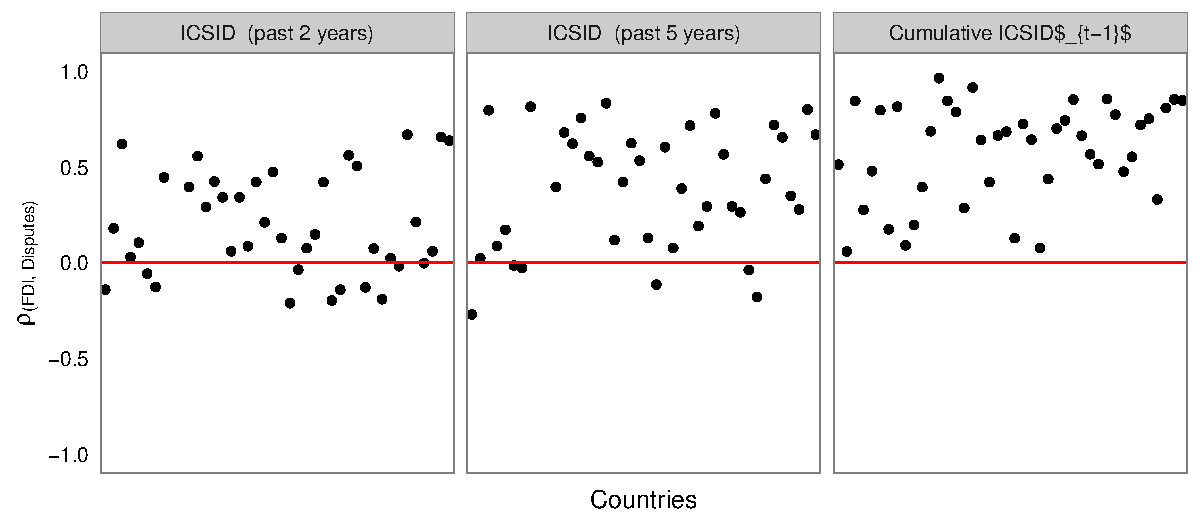
\includegraphics[width=1\textwidth]{graphics/corrFDI.pdf}
	\resizebox{1\textwidth}{!}{% Created by tikzDevice version 0.6.1 on 2016-02-24 23:26:46
% !TEX encoding = UTF-8 Unicode
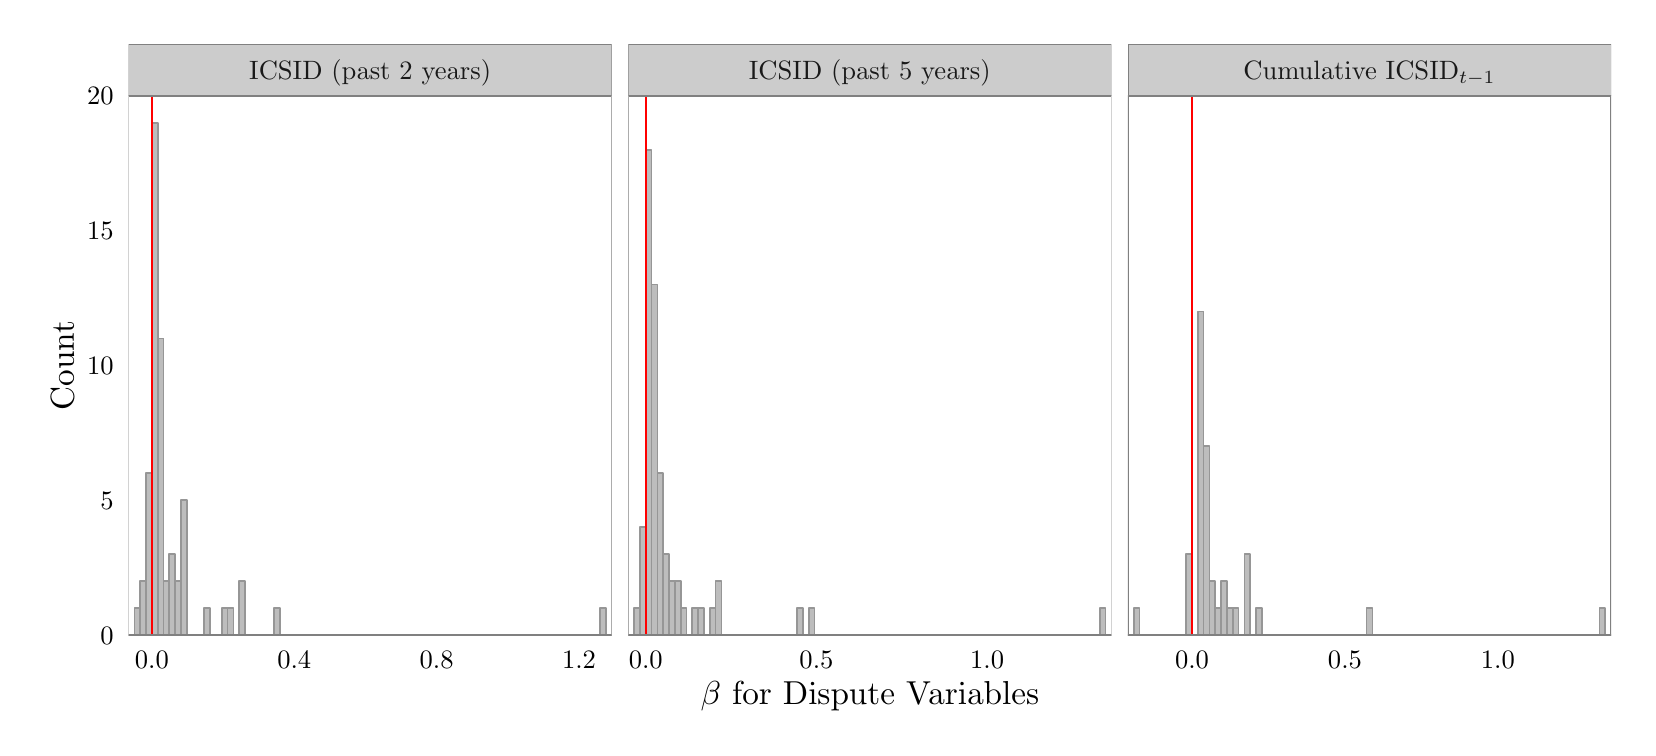
\begin{tikzpicture}[x=1pt,y=1pt]
\definecolor[named]{drawColor}{rgb}{0.00,0.00,0.00}
\definecolor[named]{fillColor}{rgb}{1.00,1.00,1.00}
\fill[color=fillColor,] (0,0) rectangle (578.16,252.94);
\begin{scope}
\path[clip] (  0.00,  0.00) rectangle (578.16,252.94);
\end{scope}
\begin{scope}
\path[clip] (  0.00,  0.00) rectangle (578.16,252.94);
\end{scope}
\begin{scope}
\path[clip] (  0.00,  0.00) rectangle (578.16,252.94);
\end{scope}
\begin{scope}
\path[clip] (  0.00,  0.00) rectangle (578.16,252.94);
\end{scope}
\begin{scope}
\path[clip] (  0.00,  0.00) rectangle (578.16,252.94);
\end{scope}
\begin{scope}
\path[clip] (  0.00,  0.00) rectangle (578.16,252.94);
\end{scope}
\begin{scope}
\path[clip] (  0.00,  0.00) rectangle (578.16,252.94);
\end{scope}
\begin{scope}
\path[clip] (  0.00,  0.00) rectangle (578.16,252.94);
\end{scope}
\begin{scope}
\path[clip] (  0.00,  0.00) rectangle (578.16,252.94);
\end{scope}
\begin{scope}
\path[clip] (  0.00,  0.00) rectangle (578.16,252.94);
\end{scope}
\begin{scope}
\path[clip] (  0.00,  0.00) rectangle (578.16,252.94);
\end{scope}
\begin{scope}
\path[clip] (  0.00,  0.00) rectangle (578.16,252.94);
\end{scope}
\begin{scope}
\path[clip] (  0.00,  0.00) rectangle (578.16,252.94);
\end{scope}
\begin{scope}
\path[clip] (  0.00,  0.00) rectangle (578.16,252.94);
\definecolor[named]{drawColor}{rgb}{1.00,1.00,1.00}
\definecolor[named]{fillColor}{rgb}{1.00,1.00,1.00}

\draw[color=drawColor,line width= 0.6pt,line cap=round,line join=round,fill=fillColor,] (  0.00,  0.00) rectangle (578.16,252.95);
\end{scope}
\begin{scope}
\path[clip] (  0.00,  0.00) rectangle (578.16,252.94);
\end{scope}
\begin{scope}
\path[clip] ( 36.46, 33.48) rectangle (211.03,228.33);
\definecolor[named]{fillColor}{rgb}{1.00,1.00,1.00}

\draw[fill=fillColor,draw opacity=0.00,] ( 36.46, 33.48) rectangle (211.03,228.33);
\definecolor[named]{drawColor}{rgb}{0.59,0.59,0.59}
\definecolor[named]{fillColor}{rgb}{0.74,0.74,0.74}

\draw[color=drawColor,line width= 0.6pt,line join=round,fill=fillColor,] ( 36.46, 33.48) rectangle ( 38.57, 33.48);

\draw[color=drawColor,line width= 0.6pt,line join=round,fill=fillColor,] ( 38.57, 33.48) rectangle ( 40.67, 43.22);

\draw[color=drawColor,line width= 0.6pt,line join=round,fill=fillColor,] ( 40.67, 33.48) rectangle ( 42.77, 52.96);

\draw[color=drawColor,line width= 0.6pt,line join=round,fill=fillColor,] ( 42.77, 33.48) rectangle ( 44.88, 91.93);

\draw[color=drawColor,line width= 0.6pt,line join=round,fill=fillColor,] ( 44.88, 33.48) rectangle ( 46.98,218.59);

\draw[color=drawColor,line width= 0.6pt,line join=round,fill=fillColor,] ( 46.98, 33.48) rectangle ( 49.08,140.65);

\draw[color=drawColor,line width= 0.6pt,line join=round,fill=fillColor,] ( 49.08, 33.48) rectangle ( 51.18, 52.96);

\draw[color=drawColor,line width= 0.6pt,line join=round,fill=fillColor,] ( 51.18, 33.48) rectangle ( 53.29, 62.70);

\draw[color=drawColor,line width= 0.6pt,line join=round,fill=fillColor,] ( 53.29, 33.48) rectangle ( 55.39, 52.96);

\draw[color=drawColor,line width= 0.6pt,line join=round,fill=fillColor,] ( 55.39, 33.48) rectangle ( 57.49, 82.19);

\draw[color=drawColor,line width= 0.6pt,line join=round,fill=fillColor,] ( 57.49, 33.48) rectangle ( 59.60, 33.48);

\draw[color=drawColor,line width= 0.6pt,line join=round,fill=fillColor,] ( 59.60, 33.48) rectangle ( 61.70, 33.48);

\draw[color=drawColor,line width= 0.6pt,line join=round,fill=fillColor,] ( 61.70, 33.48) rectangle ( 63.80, 33.48);

\draw[color=drawColor,line width= 0.6pt,line join=round,fill=fillColor,] ( 63.80, 33.48) rectangle ( 65.91, 43.22);

\draw[color=drawColor,line width= 0.6pt,line join=round,fill=fillColor,] ( 65.91, 33.48) rectangle ( 68.01, 33.48);

\draw[color=drawColor,line width= 0.6pt,line join=round,fill=fillColor,] ( 68.01, 33.48) rectangle ( 70.11, 33.48);

\draw[color=drawColor,line width= 0.6pt,line join=round,fill=fillColor,] ( 70.11, 33.48) rectangle ( 72.22, 43.22);

\draw[color=drawColor,line width= 0.6pt,line join=round,fill=fillColor,] ( 72.22, 33.48) rectangle ( 74.32, 43.22);

\draw[color=drawColor,line width= 0.6pt,line join=round,fill=fillColor,] ( 74.32, 33.48) rectangle ( 76.42, 33.48);

\draw[color=drawColor,line width= 0.6pt,line join=round,fill=fillColor,] ( 76.42, 33.48) rectangle ( 78.53, 52.96);

\draw[color=drawColor,line width= 0.6pt,line join=round,fill=fillColor,] ( 78.53, 33.48) rectangle ( 80.63, 33.48);

\draw[color=drawColor,line width= 0.6pt,line join=round,fill=fillColor,] ( 80.63, 33.48) rectangle ( 82.73, 33.48);

\draw[color=drawColor,line width= 0.6pt,line join=round,fill=fillColor,] ( 82.73, 33.48) rectangle ( 84.84, 33.48);

\draw[color=drawColor,line width= 0.6pt,line join=round,fill=fillColor,] ( 84.84, 33.48) rectangle ( 86.94, 33.48);

\draw[color=drawColor,line width= 0.6pt,line join=round,fill=fillColor,] ( 86.94, 33.48) rectangle ( 89.04, 33.48);

\draw[color=drawColor,line width= 0.6pt,line join=round,fill=fillColor,] ( 89.04, 33.48) rectangle ( 91.15, 43.22);

\draw[color=drawColor,line width= 0.6pt,line join=round,fill=fillColor,] ( 91.15, 33.48) rectangle ( 93.25, 33.48);

\draw[color=drawColor,line width= 0.6pt,line join=round,fill=fillColor,] ( 93.25, 33.48) rectangle ( 95.35, 33.48);

\draw[color=drawColor,line width= 0.6pt,line join=round,fill=fillColor,] ( 95.35, 33.48) rectangle ( 97.46, 33.48);

\draw[color=drawColor,line width= 0.6pt,line join=round,fill=fillColor,] ( 97.46, 33.48) rectangle ( 99.56, 33.48);

\draw[color=drawColor,line width= 0.6pt,line join=round,fill=fillColor,] ( 99.56, 33.48) rectangle (101.66, 33.48);

\draw[color=drawColor,line width= 0.6pt,line join=round,fill=fillColor,] (101.66, 33.48) rectangle (103.76, 33.48);

\draw[color=drawColor,line width= 0.6pt,line join=round,fill=fillColor,] (103.76, 33.48) rectangle (105.87, 33.48);

\draw[color=drawColor,line width= 0.6pt,line join=round,fill=fillColor,] (105.87, 33.48) rectangle (107.97, 33.48);

\draw[color=drawColor,line width= 0.6pt,line join=round,fill=fillColor,] (107.97, 33.48) rectangle (110.07, 33.48);

\draw[color=drawColor,line width= 0.6pt,line join=round,fill=fillColor,] (110.07, 33.48) rectangle (112.18, 33.48);

\draw[color=drawColor,line width= 0.6pt,line join=round,fill=fillColor,] (112.18, 33.48) rectangle (114.28, 33.48);

\draw[color=drawColor,line width= 0.6pt,line join=round,fill=fillColor,] (114.28, 33.48) rectangle (116.38, 33.48);

\draw[color=drawColor,line width= 0.6pt,line join=round,fill=fillColor,] (116.38, 33.48) rectangle (118.49, 33.48);

\draw[color=drawColor,line width= 0.6pt,line join=round,fill=fillColor,] (118.49, 33.48) rectangle (120.59, 33.48);

\draw[color=drawColor,line width= 0.6pt,line join=round,fill=fillColor,] (120.59, 33.48) rectangle (122.69, 33.48);

\draw[color=drawColor,line width= 0.6pt,line join=round,fill=fillColor,] (122.69, 33.48) rectangle (124.80, 33.48);

\draw[color=drawColor,line width= 0.6pt,line join=round,fill=fillColor,] (124.80, 33.48) rectangle (126.90, 33.48);

\draw[color=drawColor,line width= 0.6pt,line join=round,fill=fillColor,] (126.90, 33.48) rectangle (129.00, 33.48);

\draw[color=drawColor,line width= 0.6pt,line join=round,fill=fillColor,] (129.00, 33.48) rectangle (131.11, 33.48);

\draw[color=drawColor,line width= 0.6pt,line join=round,fill=fillColor,] (131.11, 33.48) rectangle (133.21, 33.48);

\draw[color=drawColor,line width= 0.6pt,line join=round,fill=fillColor,] (133.21, 33.48) rectangle (135.31, 33.48);

\draw[color=drawColor,line width= 0.6pt,line join=round,fill=fillColor,] (135.31, 33.48) rectangle (137.42, 33.48);

\draw[color=drawColor,line width= 0.6pt,line join=round,fill=fillColor,] (137.42, 33.48) rectangle (139.52, 33.48);

\draw[color=drawColor,line width= 0.6pt,line join=round,fill=fillColor,] (139.52, 33.48) rectangle (141.62, 33.48);

\draw[color=drawColor,line width= 0.6pt,line join=round,fill=fillColor,] (141.62, 33.48) rectangle (143.73, 33.48);

\draw[color=drawColor,line width= 0.6pt,line join=round,fill=fillColor,] (143.73, 33.48) rectangle (145.83, 33.48);

\draw[color=drawColor,line width= 0.6pt,line join=round,fill=fillColor,] (145.83, 33.48) rectangle (147.93, 33.48);

\draw[color=drawColor,line width= 0.6pt,line join=round,fill=fillColor,] (147.93, 33.48) rectangle (150.04, 33.48);

\draw[color=drawColor,line width= 0.6pt,line join=round,fill=fillColor,] (150.04, 33.48) rectangle (152.14, 33.48);

\draw[color=drawColor,line width= 0.6pt,line join=round,fill=fillColor,] (152.14, 33.48) rectangle (154.24, 33.48);

\draw[color=drawColor,line width= 0.6pt,line join=round,fill=fillColor,] (154.24, 33.48) rectangle (156.34, 33.48);

\draw[color=drawColor,line width= 0.6pt,line join=round,fill=fillColor,] (156.34, 33.48) rectangle (158.45, 33.48);

\draw[color=drawColor,line width= 0.6pt,line join=round,fill=fillColor,] (158.45, 33.48) rectangle (160.55, 33.48);

\draw[color=drawColor,line width= 0.6pt,line join=round,fill=fillColor,] (160.55, 33.48) rectangle (162.65, 33.48);

\draw[color=drawColor,line width= 0.6pt,line join=round,fill=fillColor,] (162.65, 33.48) rectangle (164.76, 33.48);

\draw[color=drawColor,line width= 0.6pt,line join=round,fill=fillColor,] (164.76, 33.48) rectangle (166.86, 33.48);

\draw[color=drawColor,line width= 0.6pt,line join=round,fill=fillColor,] (166.86, 33.48) rectangle (168.96, 33.48);

\draw[color=drawColor,line width= 0.6pt,line join=round,fill=fillColor,] (168.96, 33.48) rectangle (171.07, 33.48);

\draw[color=drawColor,line width= 0.6pt,line join=round,fill=fillColor,] (171.07, 33.48) rectangle (173.17, 33.48);

\draw[color=drawColor,line width= 0.6pt,line join=round,fill=fillColor,] (173.17, 33.48) rectangle (175.27, 33.48);

\draw[color=drawColor,line width= 0.6pt,line join=round,fill=fillColor,] (175.27, 33.48) rectangle (177.38, 33.48);

\draw[color=drawColor,line width= 0.6pt,line join=round,fill=fillColor,] (177.38, 33.48) rectangle (179.48, 33.48);

\draw[color=drawColor,line width= 0.6pt,line join=round,fill=fillColor,] (179.48, 33.48) rectangle (181.58, 33.48);

\draw[color=drawColor,line width= 0.6pt,line join=round,fill=fillColor,] (181.58, 33.48) rectangle (183.69, 33.48);

\draw[color=drawColor,line width= 0.6pt,line join=round,fill=fillColor,] (183.69, 33.48) rectangle (185.79, 33.48);

\draw[color=drawColor,line width= 0.6pt,line join=round,fill=fillColor,] (185.79, 33.48) rectangle (187.89, 33.48);

\draw[color=drawColor,line width= 0.6pt,line join=round,fill=fillColor,] (187.89, 33.48) rectangle (190.00, 33.48);

\draw[color=drawColor,line width= 0.6pt,line join=round,fill=fillColor,] (190.00, 33.48) rectangle (192.10, 33.48);

\draw[color=drawColor,line width= 0.6pt,line join=round,fill=fillColor,] (192.10, 33.48) rectangle (194.20, 33.48);

\draw[color=drawColor,line width= 0.6pt,line join=round,fill=fillColor,] (194.20, 33.48) rectangle (196.31, 33.48);

\draw[color=drawColor,line width= 0.6pt,line join=round,fill=fillColor,] (196.31, 33.48) rectangle (198.41, 33.48);

\draw[color=drawColor,line width= 0.6pt,line join=round,fill=fillColor,] (198.41, 33.48) rectangle (200.51, 33.48);

\draw[color=drawColor,line width= 0.6pt,line join=round,fill=fillColor,] (200.51, 33.48) rectangle (202.62, 33.48);

\draw[color=drawColor,line width= 0.6pt,line join=round,fill=fillColor,] (202.62, 33.48) rectangle (204.72, 33.48);

\draw[color=drawColor,line width= 0.6pt,line join=round,fill=fillColor,] (204.72, 33.48) rectangle (206.82, 33.48);

\draw[color=drawColor,line width= 0.6pt,line join=round,fill=fillColor,] (206.82, 33.48) rectangle (208.93, 43.22);

\draw[color=drawColor,line width= 0.6pt,line join=round,fill=fillColor,] (208.93, 33.48) rectangle (211.03, 33.48);
\definecolor[named]{drawColor}{rgb}{1.00,0.00,0.00}
\definecolor[named]{fillColor}{rgb}{1.00,0.00,0.00}

\draw[color=drawColor,line width= 0.6pt,line join=round,fill=fillColor,] ( 44.88, 33.48) -- ( 44.88,228.33);
\definecolor[named]{drawColor}{rgb}{0.50,0.50,0.50}

\draw[color=drawColor,line width= 0.6pt,line cap=round,line join=round,fill opacity=0.00,] ( 36.46, 33.48) rectangle (211.03,228.33);
\end{scope}
\begin{scope}
\path[clip] (  0.00,  0.00) rectangle (578.16,252.94);
\end{scope}
\begin{scope}
\path[clip] (217.03, 33.48) rectangle (391.59,228.33);
\definecolor[named]{fillColor}{rgb}{1.00,1.00,1.00}

\draw[fill=fillColor,draw opacity=0.00,] (217.03, 33.48) rectangle (391.59,228.33);
\definecolor[named]{drawColor}{rgb}{0.59,0.59,0.59}
\definecolor[named]{fillColor}{rgb}{0.74,0.74,0.74}

\draw[color=drawColor,line width= 0.6pt,line join=round,fill=fillColor,] (217.03, 33.48) rectangle (219.13, 33.48);

\draw[color=drawColor,line width= 0.6pt,line join=round,fill=fillColor,] (219.13, 33.48) rectangle (221.23, 43.22);

\draw[color=drawColor,line width= 0.6pt,line join=round,fill=fillColor,] (221.23, 33.48) rectangle (223.34, 72.45);

\draw[color=drawColor,line width= 0.6pt,line join=round,fill=fillColor,] (223.34, 33.48) rectangle (225.44,208.85);

\draw[color=drawColor,line width= 0.6pt,line join=round,fill=fillColor,] (225.44, 33.48) rectangle (227.54,160.13);

\draw[color=drawColor,line width= 0.6pt,line join=round,fill=fillColor,] (227.54, 33.48) rectangle (229.65, 91.93);

\draw[color=drawColor,line width= 0.6pt,line join=round,fill=fillColor,] (229.65, 33.48) rectangle (231.75, 62.70);

\draw[color=drawColor,line width= 0.6pt,line join=round,fill=fillColor,] (231.75, 33.48) rectangle (233.85, 52.96);

\draw[color=drawColor,line width= 0.6pt,line join=round,fill=fillColor,] (233.85, 33.48) rectangle (235.96, 52.96);

\draw[color=drawColor,line width= 0.6pt,line join=round,fill=fillColor,] (235.96, 33.48) rectangle (238.06, 43.22);

\draw[color=drawColor,line width= 0.6pt,line join=round,fill=fillColor,] (238.06, 33.48) rectangle (240.16, 33.48);

\draw[color=drawColor,line width= 0.6pt,line join=round,fill=fillColor,] (240.16, 33.48) rectangle (242.27, 43.22);

\draw[color=drawColor,line width= 0.6pt,line join=round,fill=fillColor,] (242.27, 33.48) rectangle (244.37, 43.22);

\draw[color=drawColor,line width= 0.6pt,line join=round,fill=fillColor,] (244.37, 33.48) rectangle (246.47, 33.48);

\draw[color=drawColor,line width= 0.6pt,line join=round,fill=fillColor,] (246.47, 33.48) rectangle (248.58, 43.22);

\draw[color=drawColor,line width= 0.6pt,line join=round,fill=fillColor,] (248.58, 33.48) rectangle (250.68, 52.96);

\draw[color=drawColor,line width= 0.6pt,line join=round,fill=fillColor,] (250.68, 33.48) rectangle (252.78, 33.48);

\draw[color=drawColor,line width= 0.6pt,line join=round,fill=fillColor,] (252.78, 33.48) rectangle (254.89, 33.48);

\draw[color=drawColor,line width= 0.6pt,line join=round,fill=fillColor,] (254.89, 33.48) rectangle (256.99, 33.48);

\draw[color=drawColor,line width= 0.6pt,line join=round,fill=fillColor,] (256.99, 33.48) rectangle (259.09, 33.48);

\draw[color=drawColor,line width= 0.6pt,line join=round,fill=fillColor,] (259.09, 33.48) rectangle (261.20, 33.48);

\draw[color=drawColor,line width= 0.6pt,line join=round,fill=fillColor,] (261.20, 33.48) rectangle (263.30, 33.48);

\draw[color=drawColor,line width= 0.6pt,line join=round,fill=fillColor,] (263.30, 33.48) rectangle (265.40, 33.48);

\draw[color=drawColor,line width= 0.6pt,line join=round,fill=fillColor,] (265.40, 33.48) rectangle (267.51, 33.48);

\draw[color=drawColor,line width= 0.6pt,line join=round,fill=fillColor,] (267.51, 33.48) rectangle (269.61, 33.48);

\draw[color=drawColor,line width= 0.6pt,line join=round,fill=fillColor,] (269.61, 33.48) rectangle (271.71, 33.48);

\draw[color=drawColor,line width= 0.6pt,line join=round,fill=fillColor,] (271.71, 33.48) rectangle (273.81, 33.48);

\draw[color=drawColor,line width= 0.6pt,line join=round,fill=fillColor,] (273.81, 33.48) rectangle (275.92, 33.48);

\draw[color=drawColor,line width= 0.6pt,line join=round,fill=fillColor,] (275.92, 33.48) rectangle (278.02, 33.48);

\draw[color=drawColor,line width= 0.6pt,line join=round,fill=fillColor,] (278.02, 33.48) rectangle (280.12, 43.22);

\draw[color=drawColor,line width= 0.6pt,line join=round,fill=fillColor,] (280.12, 33.48) rectangle (282.23, 33.48);

\draw[color=drawColor,line width= 0.6pt,line join=round,fill=fillColor,] (282.23, 33.48) rectangle (284.33, 43.22);

\draw[color=drawColor,line width= 0.6pt,line join=round,fill=fillColor,] (284.33, 33.48) rectangle (286.43, 33.48);

\draw[color=drawColor,line width= 0.6pt,line join=round,fill=fillColor,] (286.43, 33.48) rectangle (288.54, 33.48);

\draw[color=drawColor,line width= 0.6pt,line join=round,fill=fillColor,] (288.54, 33.48) rectangle (290.64, 33.48);

\draw[color=drawColor,line width= 0.6pt,line join=round,fill=fillColor,] (290.64, 33.48) rectangle (292.74, 33.48);

\draw[color=drawColor,line width= 0.6pt,line join=round,fill=fillColor,] (292.74, 33.48) rectangle (294.85, 33.48);

\draw[color=drawColor,line width= 0.6pt,line join=round,fill=fillColor,] (294.85, 33.48) rectangle (296.95, 33.48);

\draw[color=drawColor,line width= 0.6pt,line join=round,fill=fillColor,] (296.95, 33.48) rectangle (299.05, 33.48);

\draw[color=drawColor,line width= 0.6pt,line join=round,fill=fillColor,] (299.05, 33.48) rectangle (301.16, 33.48);

\draw[color=drawColor,line width= 0.6pt,line join=round,fill=fillColor,] (301.16, 33.48) rectangle (303.26, 33.48);

\draw[color=drawColor,line width= 0.6pt,line join=round,fill=fillColor,] (303.26, 33.48) rectangle (305.36, 33.48);

\draw[color=drawColor,line width= 0.6pt,line join=round,fill=fillColor,] (305.36, 33.48) rectangle (307.47, 33.48);

\draw[color=drawColor,line width= 0.6pt,line join=round,fill=fillColor,] (307.47, 33.48) rectangle (309.57, 33.48);

\draw[color=drawColor,line width= 0.6pt,line join=round,fill=fillColor,] (309.57, 33.48) rectangle (311.67, 33.48);

\draw[color=drawColor,line width= 0.6pt,line join=round,fill=fillColor,] (311.67, 33.48) rectangle (313.78, 33.48);

\draw[color=drawColor,line width= 0.6pt,line join=round,fill=fillColor,] (313.78, 33.48) rectangle (315.88, 33.48);

\draw[color=drawColor,line width= 0.6pt,line join=round,fill=fillColor,] (315.88, 33.48) rectangle (317.98, 33.48);

\draw[color=drawColor,line width= 0.6pt,line join=round,fill=fillColor,] (317.98, 33.48) rectangle (320.09, 33.48);

\draw[color=drawColor,line width= 0.6pt,line join=round,fill=fillColor,] (320.09, 33.48) rectangle (322.19, 33.48);

\draw[color=drawColor,line width= 0.6pt,line join=round,fill=fillColor,] (322.19, 33.48) rectangle (324.29, 33.48);

\draw[color=drawColor,line width= 0.6pt,line join=round,fill=fillColor,] (324.29, 33.48) rectangle (326.39, 33.48);

\draw[color=drawColor,line width= 0.6pt,line join=round,fill=fillColor,] (326.39, 33.48) rectangle (328.50, 33.48);

\draw[color=drawColor,line width= 0.6pt,line join=round,fill=fillColor,] (328.50, 33.48) rectangle (330.60, 33.48);

\draw[color=drawColor,line width= 0.6pt,line join=round,fill=fillColor,] (330.60, 33.48) rectangle (332.70, 33.48);

\draw[color=drawColor,line width= 0.6pt,line join=round,fill=fillColor,] (332.70, 33.48) rectangle (334.81, 33.48);

\draw[color=drawColor,line width= 0.6pt,line join=round,fill=fillColor,] (334.81, 33.48) rectangle (336.91, 33.48);

\draw[color=drawColor,line width= 0.6pt,line join=round,fill=fillColor,] (336.91, 33.48) rectangle (339.01, 33.48);

\draw[color=drawColor,line width= 0.6pt,line join=round,fill=fillColor,] (339.01, 33.48) rectangle (341.12, 33.48);

\draw[color=drawColor,line width= 0.6pt,line join=round,fill=fillColor,] (341.12, 33.48) rectangle (343.22, 33.48);

\draw[color=drawColor,line width= 0.6pt,line join=round,fill=fillColor,] (343.22, 33.48) rectangle (345.32, 33.48);

\draw[color=drawColor,line width= 0.6pt,line join=round,fill=fillColor,] (345.32, 33.48) rectangle (347.43, 33.48);

\draw[color=drawColor,line width= 0.6pt,line join=round,fill=fillColor,] (347.43, 33.48) rectangle (349.53, 33.48);

\draw[color=drawColor,line width= 0.6pt,line join=round,fill=fillColor,] (349.53, 33.48) rectangle (351.63, 33.48);

\draw[color=drawColor,line width= 0.6pt,line join=round,fill=fillColor,] (351.63, 33.48) rectangle (353.74, 33.48);

\draw[color=drawColor,line width= 0.6pt,line join=round,fill=fillColor,] (353.74, 33.48) rectangle (355.84, 33.48);

\draw[color=drawColor,line width= 0.6pt,line join=round,fill=fillColor,] (355.84, 33.48) rectangle (357.94, 33.48);

\draw[color=drawColor,line width= 0.6pt,line join=round,fill=fillColor,] (357.94, 33.48) rectangle (360.05, 33.48);

\draw[color=drawColor,line width= 0.6pt,line join=round,fill=fillColor,] (360.05, 33.48) rectangle (362.15, 33.48);

\draw[color=drawColor,line width= 0.6pt,line join=round,fill=fillColor,] (362.15, 33.48) rectangle (364.25, 33.48);

\draw[color=drawColor,line width= 0.6pt,line join=round,fill=fillColor,] (364.25, 33.48) rectangle (366.36, 33.48);

\draw[color=drawColor,line width= 0.6pt,line join=round,fill=fillColor,] (366.36, 33.48) rectangle (368.46, 33.48);

\draw[color=drawColor,line width= 0.6pt,line join=round,fill=fillColor,] (368.46, 33.48) rectangle (370.56, 33.48);

\draw[color=drawColor,line width= 0.6pt,line join=round,fill=fillColor,] (370.56, 33.48) rectangle (372.67, 33.48);

\draw[color=drawColor,line width= 0.6pt,line join=round,fill=fillColor,] (372.67, 33.48) rectangle (374.77, 33.48);

\draw[color=drawColor,line width= 0.6pt,line join=round,fill=fillColor,] (374.77, 33.48) rectangle (376.87, 33.48);

\draw[color=drawColor,line width= 0.6pt,line join=round,fill=fillColor,] (376.87, 33.48) rectangle (378.97, 33.48);

\draw[color=drawColor,line width= 0.6pt,line join=round,fill=fillColor,] (378.97, 33.48) rectangle (381.08, 33.48);

\draw[color=drawColor,line width= 0.6pt,line join=round,fill=fillColor,] (381.08, 33.48) rectangle (383.18, 33.48);

\draw[color=drawColor,line width= 0.6pt,line join=round,fill=fillColor,] (383.18, 33.48) rectangle (385.28, 33.48);

\draw[color=drawColor,line width= 0.6pt,line join=round,fill=fillColor,] (385.28, 33.48) rectangle (387.39, 33.48);

\draw[color=drawColor,line width= 0.6pt,line join=round,fill=fillColor,] (387.39, 33.48) rectangle (389.49, 43.22);

\draw[color=drawColor,line width= 0.6pt,line join=round,fill=fillColor,] (389.49, 33.48) rectangle (391.59, 33.48);
\definecolor[named]{drawColor}{rgb}{1.00,0.00,0.00}
\definecolor[named]{fillColor}{rgb}{1.00,0.00,0.00}

\draw[color=drawColor,line width= 0.6pt,line join=round,fill=fillColor,] (223.34, 33.48) -- (223.34,228.33);
\definecolor[named]{drawColor}{rgb}{0.50,0.50,0.50}

\draw[color=drawColor,line width= 0.6pt,line cap=round,line join=round,fill opacity=0.00,] (217.03, 33.48) rectangle (391.59,228.33);
\end{scope}
\begin{scope}
\path[clip] (  0.00,  0.00) rectangle (578.16,252.94);
\end{scope}
\begin{scope}
\path[clip] (397.59, 33.48) rectangle (572.16,228.33);
\definecolor[named]{fillColor}{rgb}{1.00,1.00,1.00}

\draw[fill=fillColor,draw opacity=0.00,] (397.59, 33.48) rectangle (572.16,228.33);
\definecolor[named]{drawColor}{rgb}{0.59,0.59,0.59}
\definecolor[named]{fillColor}{rgb}{0.74,0.74,0.74}

\draw[color=drawColor,line width= 0.6pt,line join=round,fill=fillColor,] (397.59, 33.48) rectangle (399.70, 33.48);

\draw[color=drawColor,line width= 0.6pt,line join=round,fill=fillColor,] (399.70, 33.48) rectangle (401.80, 43.22);

\draw[color=drawColor,line width= 0.6pt,line join=round,fill=fillColor,] (401.80, 33.48) rectangle (403.90, 33.48);

\draw[color=drawColor,line width= 0.6pt,line join=round,fill=fillColor,] (403.90, 33.48) rectangle (406.01, 33.48);

\draw[color=drawColor,line width= 0.6pt,line join=round,fill=fillColor,] (406.01, 33.48) rectangle (408.11, 33.48);

\draw[color=drawColor,line width= 0.6pt,line join=round,fill=fillColor,] (408.11, 33.48) rectangle (410.21, 33.48);

\draw[color=drawColor,line width= 0.6pt,line join=round,fill=fillColor,] (410.21, 33.48) rectangle (412.32, 33.48);

\draw[color=drawColor,line width= 0.6pt,line join=round,fill=fillColor,] (412.32, 33.48) rectangle (414.42, 33.48);

\draw[color=drawColor,line width= 0.6pt,line join=round,fill=fillColor,] (414.42, 33.48) rectangle (416.52, 33.48);

\draw[color=drawColor,line width= 0.6pt,line join=round,fill=fillColor,] (416.52, 33.48) rectangle (418.63, 33.48);

\draw[color=drawColor,line width= 0.6pt,line join=round,fill=fillColor,] (418.63, 33.48) rectangle (420.73, 62.70);

\draw[color=drawColor,line width= 0.6pt,line join=round,fill=fillColor,] (422.83, 33.48) rectangle (424.94,150.39);

\draw[color=drawColor,line width= 0.6pt,line join=round,fill=fillColor,] (424.94, 33.48) rectangle (427.04,101.68);

\draw[color=drawColor,line width= 0.6pt,line join=round,fill=fillColor,] (427.04, 33.48) rectangle (429.14, 52.96);

\draw[color=drawColor,line width= 0.6pt,line join=round,fill=fillColor,] (429.14, 33.48) rectangle (431.25, 43.22);

\draw[color=drawColor,line width= 0.6pt,line join=round,fill=fillColor,] (431.25, 33.48) rectangle (433.35, 52.96);

\draw[color=drawColor,line width= 0.6pt,line join=round,fill=fillColor,] (433.35, 33.48) rectangle (435.45, 43.22);

\draw[color=drawColor,line width= 0.6pt,line join=round,fill=fillColor,] (435.45, 33.48) rectangle (437.55, 43.22);

\draw[color=drawColor,line width= 0.6pt,line join=round,fill=fillColor,] (437.55, 33.48) rectangle (439.66, 33.48);

\draw[color=drawColor,line width= 0.6pt,line join=round,fill=fillColor,] (439.66, 33.48) rectangle (441.76, 62.70);

\draw[color=drawColor,line width= 0.6pt,line join=round,fill=fillColor,] (441.76, 33.48) rectangle (443.86, 33.48);

\draw[color=drawColor,line width= 0.6pt,line join=round,fill=fillColor,] (443.86, 33.48) rectangle (445.97, 43.22);

\draw[color=drawColor,line width= 0.6pt,line join=round,fill=fillColor,] (445.97, 33.48) rectangle (448.07, 33.48);

\draw[color=drawColor,line width= 0.6pt,line join=round,fill=fillColor,] (448.07, 33.48) rectangle (450.17, 33.48);

\draw[color=drawColor,line width= 0.6pt,line join=round,fill=fillColor,] (450.17, 33.48) rectangle (452.28, 33.48);

\draw[color=drawColor,line width= 0.6pt,line join=round,fill=fillColor,] (452.28, 33.48) rectangle (454.38, 33.48);

\draw[color=drawColor,line width= 0.6pt,line join=round,fill=fillColor,] (454.38, 33.48) rectangle (456.48, 33.48);

\draw[color=drawColor,line width= 0.6pt,line join=round,fill=fillColor,] (456.48, 33.48) rectangle (458.59, 33.48);

\draw[color=drawColor,line width= 0.6pt,line join=round,fill=fillColor,] (458.59, 33.48) rectangle (460.69, 33.48);

\draw[color=drawColor,line width= 0.6pt,line join=round,fill=fillColor,] (460.69, 33.48) rectangle (462.79, 33.48);

\draw[color=drawColor,line width= 0.6pt,line join=round,fill=fillColor,] (462.79, 33.48) rectangle (464.90, 33.48);

\draw[color=drawColor,line width= 0.6pt,line join=round,fill=fillColor,] (464.90, 33.48) rectangle (467.00, 33.48);

\draw[color=drawColor,line width= 0.6pt,line join=round,fill=fillColor,] (467.00, 33.48) rectangle (469.10, 33.48);

\draw[color=drawColor,line width= 0.6pt,line join=round,fill=fillColor,] (469.10, 33.48) rectangle (471.21, 33.48);

\draw[color=drawColor,line width= 0.6pt,line join=round,fill=fillColor,] (471.21, 33.48) rectangle (473.31, 33.48);

\draw[color=drawColor,line width= 0.6pt,line join=round,fill=fillColor,] (473.31, 33.48) rectangle (475.41, 33.48);

\draw[color=drawColor,line width= 0.6pt,line join=round,fill=fillColor,] (475.41, 33.48) rectangle (477.52, 33.48);

\draw[color=drawColor,line width= 0.6pt,line join=round,fill=fillColor,] (477.52, 33.48) rectangle (479.62, 33.48);

\draw[color=drawColor,line width= 0.6pt,line join=round,fill=fillColor,] (479.62, 33.48) rectangle (481.72, 33.48);

\draw[color=drawColor,line width= 0.6pt,line join=round,fill=fillColor,] (481.72, 33.48) rectangle (483.83, 33.48);

\draw[color=drawColor,line width= 0.6pt,line join=round,fill=fillColor,] (483.83, 33.48) rectangle (485.93, 43.22);

\draw[color=drawColor,line width= 0.6pt,line join=round,fill=fillColor,] (485.93, 33.48) rectangle (488.03, 33.48);

\draw[color=drawColor,line width= 0.6pt,line join=round,fill=fillColor,] (488.03, 33.48) rectangle (490.14, 33.48);

\draw[color=drawColor,line width= 0.6pt,line join=round,fill=fillColor,] (490.14, 33.48) rectangle (492.24, 33.48);

\draw[color=drawColor,line width= 0.6pt,line join=round,fill=fillColor,] (492.24, 33.48) rectangle (494.34, 33.48);

\draw[color=drawColor,line width= 0.6pt,line join=round,fill=fillColor,] (494.34, 33.48) rectangle (496.44, 33.48);

\draw[color=drawColor,line width= 0.6pt,line join=round,fill=fillColor,] (496.44, 33.48) rectangle (498.55, 33.48);

\draw[color=drawColor,line width= 0.6pt,line join=round,fill=fillColor,] (498.55, 33.48) rectangle (500.65, 33.48);

\draw[color=drawColor,line width= 0.6pt,line join=round,fill=fillColor,] (500.65, 33.48) rectangle (502.75, 33.48);

\draw[color=drawColor,line width= 0.6pt,line join=round,fill=fillColor,] (502.75, 33.48) rectangle (504.86, 33.48);

\draw[color=drawColor,line width= 0.6pt,line join=round,fill=fillColor,] (504.86, 33.48) rectangle (506.96, 33.48);

\draw[color=drawColor,line width= 0.6pt,line join=round,fill=fillColor,] (506.96, 33.48) rectangle (509.06, 33.48);

\draw[color=drawColor,line width= 0.6pt,line join=round,fill=fillColor,] (509.06, 33.48) rectangle (511.17, 33.48);

\draw[color=drawColor,line width= 0.6pt,line join=round,fill=fillColor,] (511.17, 33.48) rectangle (513.27, 33.48);

\draw[color=drawColor,line width= 0.6pt,line join=round,fill=fillColor,] (513.27, 33.48) rectangle (515.37, 33.48);

\draw[color=drawColor,line width= 0.6pt,line join=round,fill=fillColor,] (515.37, 33.48) rectangle (517.48, 33.48);

\draw[color=drawColor,line width= 0.6pt,line join=round,fill=fillColor,] (517.48, 33.48) rectangle (519.58, 33.48);

\draw[color=drawColor,line width= 0.6pt,line join=round,fill=fillColor,] (519.58, 33.48) rectangle (521.68, 33.48);

\draw[color=drawColor,line width= 0.6pt,line join=round,fill=fillColor,] (521.68, 33.48) rectangle (523.79, 33.48);

\draw[color=drawColor,line width= 0.6pt,line join=round,fill=fillColor,] (523.79, 33.48) rectangle (525.89, 33.48);

\draw[color=drawColor,line width= 0.6pt,line join=round,fill=fillColor,] (525.89, 33.48) rectangle (527.99, 33.48);

\draw[color=drawColor,line width= 0.6pt,line join=round,fill=fillColor,] (527.99, 33.48) rectangle (530.10, 33.48);

\draw[color=drawColor,line width= 0.6pt,line join=round,fill=fillColor,] (530.10, 33.48) rectangle (532.20, 33.48);

\draw[color=drawColor,line width= 0.6pt,line join=round,fill=fillColor,] (532.20, 33.48) rectangle (534.30, 33.48);

\draw[color=drawColor,line width= 0.6pt,line join=round,fill=fillColor,] (534.30, 33.48) rectangle (536.41, 33.48);

\draw[color=drawColor,line width= 0.6pt,line join=round,fill=fillColor,] (536.41, 33.48) rectangle (538.51, 33.48);

\draw[color=drawColor,line width= 0.6pt,line join=round,fill=fillColor,] (538.51, 33.48) rectangle (540.61, 33.48);

\draw[color=drawColor,line width= 0.6pt,line join=round,fill=fillColor,] (540.61, 33.48) rectangle (542.72, 33.48);

\draw[color=drawColor,line width= 0.6pt,line join=round,fill=fillColor,] (542.72, 33.48) rectangle (544.82, 33.48);

\draw[color=drawColor,line width= 0.6pt,line join=round,fill=fillColor,] (544.82, 33.48) rectangle (546.92, 33.48);

\draw[color=drawColor,line width= 0.6pt,line join=round,fill=fillColor,] (546.92, 33.48) rectangle (549.02, 33.48);

\draw[color=drawColor,line width= 0.6pt,line join=round,fill=fillColor,] (549.02, 33.48) rectangle (551.13, 33.48);

\draw[color=drawColor,line width= 0.6pt,line join=round,fill=fillColor,] (551.13, 33.48) rectangle (553.23, 33.48);

\draw[color=drawColor,line width= 0.6pt,line join=round,fill=fillColor,] (553.23, 33.48) rectangle (555.33, 33.48);

\draw[color=drawColor,line width= 0.6pt,line join=round,fill=fillColor,] (555.33, 33.48) rectangle (557.44, 33.48);

\draw[color=drawColor,line width= 0.6pt,line join=round,fill=fillColor,] (557.44, 33.48) rectangle (559.54, 33.48);

\draw[color=drawColor,line width= 0.6pt,line join=round,fill=fillColor,] (559.54, 33.48) rectangle (561.64, 33.48);

\draw[color=drawColor,line width= 0.6pt,line join=round,fill=fillColor,] (561.64, 33.48) rectangle (563.75, 33.48);

\draw[color=drawColor,line width= 0.6pt,line join=round,fill=fillColor,] (563.75, 33.48) rectangle (565.85, 33.48);

\draw[color=drawColor,line width= 0.6pt,line join=round,fill=fillColor,] (565.85, 33.48) rectangle (567.95, 33.48);

\draw[color=drawColor,line width= 0.6pt,line join=round,fill=fillColor,] (567.95, 33.48) rectangle (570.06, 43.22);

\draw[color=drawColor,line width= 0.6pt,line join=round,fill=fillColor,] (570.06, 33.48) rectangle (572.16, 33.48);
\definecolor[named]{drawColor}{rgb}{1.00,0.00,0.00}
\definecolor[named]{fillColor}{rgb}{1.00,0.00,0.00}

\draw[color=drawColor,line width= 0.6pt,line join=round,fill=fillColor,] (420.73, 33.48) -- (420.73,228.33);
\definecolor[named]{drawColor}{rgb}{0.50,0.50,0.50}

\draw[color=drawColor,line width= 0.6pt,line cap=round,line join=round,fill opacity=0.00,] (397.59, 33.48) rectangle (572.16,228.33);
\end{scope}
\begin{scope}
\path[clip] (  0.00,  0.00) rectangle (578.16,252.94);
\end{scope}
\begin{scope}
\path[clip] (  0.00,  0.00) rectangle (578.16,252.94);
\end{scope}
\begin{scope}
\path[clip] (  0.00,  0.00) rectangle (578.16,252.94);
\end{scope}
\begin{scope}
\path[clip] ( 36.46,228.33) rectangle (211.03,246.95);
\definecolor[named]{drawColor}{rgb}{0.50,0.50,0.50}
\definecolor[named]{fillColor}{rgb}{0.80,0.80,0.80}

\draw[color=drawColor,line width= 0.2pt,line cap=round,line join=round,fill=fillColor,] ( 36.46,228.33) rectangle (211.03,246.95);
\definecolor[named]{drawColor}{rgb}{0.10,0.10,0.10}

\node[color=drawColor,anchor=base,inner sep=0pt, outer sep=0pt, scale=  0.96] at (123.75,234.33) {ICSID  (past 2 years)%
};
\end{scope}
\begin{scope}
\path[clip] ( 36.46,228.33) rectangle (211.03,246.95);
\end{scope}
\begin{scope}
\path[clip] (  0.00,  0.00) rectangle (578.16,252.94);
\end{scope}
\begin{scope}
\path[clip] (  0.00,  0.00) rectangle (578.16,252.94);
\end{scope}
\begin{scope}
\path[clip] (  0.00,  0.00) rectangle (578.16,252.94);
\end{scope}
\begin{scope}
\path[clip] (  0.00,  0.00) rectangle (578.16,252.94);
\end{scope}
\begin{scope}
\path[clip] (  0.00,  0.00) rectangle (578.16,252.94);
\end{scope}
\begin{scope}
\path[clip] (  0.00,  0.00) rectangle (578.16,252.94);
\end{scope}
\begin{scope}
\path[clip] (217.03,228.33) rectangle (391.59,246.95);
\definecolor[named]{drawColor}{rgb}{0.50,0.50,0.50}
\definecolor[named]{fillColor}{rgb}{0.80,0.80,0.80}

\draw[color=drawColor,line width= 0.2pt,line cap=round,line join=round,fill=fillColor,] (217.03,228.33) rectangle (391.59,246.95);
\definecolor[named]{drawColor}{rgb}{0.10,0.10,0.10}

\node[color=drawColor,anchor=base,inner sep=0pt, outer sep=0pt, scale=  0.96] at (304.31,234.33) {ICSID  (past 5 years)%
};
\end{scope}
\begin{scope}
\path[clip] (217.03,228.33) rectangle (391.59,246.95);
\end{scope}
\begin{scope}
\path[clip] (  0.00,  0.00) rectangle (578.16,252.94);
\end{scope}
\begin{scope}
\path[clip] (  0.00,  0.00) rectangle (578.16,252.94);
\end{scope}
\begin{scope}
\path[clip] (  0.00,  0.00) rectangle (578.16,252.94);
\end{scope}
\begin{scope}
\path[clip] (  0.00,  0.00) rectangle (578.16,252.94);
\end{scope}
\begin{scope}
\path[clip] (  0.00,  0.00) rectangle (578.16,252.94);
\end{scope}
\begin{scope}
\path[clip] (  0.00,  0.00) rectangle (578.16,252.94);
\end{scope}
\begin{scope}
\path[clip] (397.59,228.33) rectangle (572.16,246.95);
\definecolor[named]{drawColor}{rgb}{0.50,0.50,0.50}
\definecolor[named]{fillColor}{rgb}{0.80,0.80,0.80}

\draw[color=drawColor,line width= 0.2pt,line cap=round,line join=round,fill=fillColor,] (397.59,228.33) rectangle (572.16,246.95);
\definecolor[named]{drawColor}{rgb}{0.10,0.10,0.10}

\node[color=drawColor,anchor=base,inner sep=0pt, outer sep=0pt, scale=  0.96] at (484.88,234.33) {Cumulative ICSID$_{t-1}$%
};
\end{scope}
\begin{scope}
\path[clip] (397.59,228.33) rectangle (572.16,246.95);
\end{scope}
\begin{scope}
\path[clip] (  0.00,  0.00) rectangle (578.16,252.94);
\end{scope}
\begin{scope}
\path[clip] (  0.00,  0.00) rectangle (578.16,252.94);
\end{scope}
\begin{scope}
\path[clip] (  0.00,  0.00) rectangle (578.16,252.94);
\end{scope}
\begin{scope}
\path[clip] (  0.00,  0.00) rectangle (578.16,252.94);
\end{scope}
\begin{scope}
\path[clip] (  0.00,  0.00) rectangle (578.16,252.94);
\end{scope}
\begin{scope}
\path[clip] (  0.00,  0.00) rectangle (578.16,252.94);
\end{scope}
\begin{scope}
\path[clip] (  0.00,  0.00) rectangle (578.16,252.94);
\end{scope}
\begin{scope}
\path[clip] (  0.00,  0.00) rectangle (578.16,252.94);
\end{scope}
\begin{scope}
\path[clip] (  0.00,  0.00) rectangle (578.16,252.94);
\definecolor[named]{drawColor}{rgb}{0.00,0.00,0.00}

\node[color=drawColor,anchor=base east,inner sep=0pt, outer sep=0pt, scale=  0.96] at ( 31.06, 30.17) {0%
};

\node[color=drawColor,anchor=base east,inner sep=0pt, outer sep=0pt, scale=  0.96] at ( 31.06, 78.88) {5%
};

\node[color=drawColor,anchor=base east,inner sep=0pt, outer sep=0pt, scale=  0.96] at ( 31.06,127.60) {10%
};

\node[color=drawColor,anchor=base east,inner sep=0pt, outer sep=0pt, scale=  0.96] at ( 31.06,176.31) {15%
};

\node[color=drawColor,anchor=base east,inner sep=0pt, outer sep=0pt, scale=  0.96] at ( 31.06,225.03) {20%
};
\end{scope}
\begin{scope}
\path[clip] (  0.00,  0.00) rectangle (578.16,252.94);
\end{scope}
\begin{scope}
\path[clip] (  0.00,  0.00) rectangle (578.16,252.94);
\end{scope}
\begin{scope}
\path[clip] (  0.00,  0.00) rectangle (578.16,252.94);
\end{scope}
\begin{scope}
\path[clip] (  0.00,  0.00) rectangle (578.16,252.94);
\end{scope}
\begin{scope}
\path[clip] (  0.00,  0.00) rectangle (578.16,252.94);
\end{scope}
\begin{scope}
\path[clip] (  0.00,  0.00) rectangle (578.16,252.94);
\end{scope}
\begin{scope}
\path[clip] (  0.00,  0.00) rectangle (578.16,252.94);
\end{scope}
\begin{scope}
\path[clip] (  0.00,  0.00) rectangle (578.16,252.94);
\end{scope}
\begin{scope}
\path[clip] (  0.00,  0.00) rectangle (578.16,252.94);
\end{scope}
\begin{scope}
\path[clip] (  0.00,  0.00) rectangle (578.16,252.94);
\end{scope}
\begin{scope}
\path[clip] (  0.00,  0.00) rectangle (578.16,252.94);
\end{scope}
\begin{scope}
\path[clip] (  0.00,  0.00) rectangle (578.16,252.94);
\end{scope}
\begin{scope}
\path[clip] (  0.00,  0.00) rectangle (578.16,252.94);
\end{scope}
\begin{scope}
\path[clip] (  0.00,  0.00) rectangle (578.16,252.94);
\end{scope}
\begin{scope}
\path[clip] (  0.00,  0.00) rectangle (578.16,252.94);
\end{scope}
\begin{scope}
\path[clip] (  0.00,  0.00) rectangle (578.16,252.94);
\end{scope}
\begin{scope}
\path[clip] (  0.00,  0.00) rectangle (578.16,252.94);
\end{scope}
\begin{scope}
\path[clip] (  0.00,  0.00) rectangle (578.16,252.94);
\definecolor[named]{drawColor}{rgb}{0.00,0.00,0.00}

\node[color=drawColor,anchor=base,inner sep=0pt, outer sep=0pt, scale=  0.96] at ( 44.88, 21.46) {0.0%
};

\node[color=drawColor,anchor=base,inner sep=0pt, outer sep=0pt, scale=  0.96] at ( 96.32, 21.46) {0.4%
};

\node[color=drawColor,anchor=base,inner sep=0pt, outer sep=0pt, scale=  0.96] at (147.76, 21.46) {0.8%
};

\node[color=drawColor,anchor=base,inner sep=0pt, outer sep=0pt, scale=  0.96] at (199.21, 21.46) {1.2%
};
\end{scope}
\begin{scope}
\path[clip] (  0.00,  0.00) rectangle (578.16,252.94);
\end{scope}
\begin{scope}
\path[clip] (  0.00,  0.00) rectangle (578.16,252.94);
\end{scope}
\begin{scope}
\path[clip] (  0.00,  0.00) rectangle (578.16,252.94);
\end{scope}
\begin{scope}
\path[clip] (  0.00,  0.00) rectangle (578.16,252.94);
\end{scope}
\begin{scope}
\path[clip] (  0.00,  0.00) rectangle (578.16,252.94);
\end{scope}
\begin{scope}
\path[clip] (  0.00,  0.00) rectangle (578.16,252.94);
\end{scope}
\begin{scope}
\path[clip] (  0.00,  0.00) rectangle (578.16,252.94);
\end{scope}
\begin{scope}
\path[clip] (  0.00,  0.00) rectangle (578.16,252.94);
\end{scope}
\begin{scope}
\path[clip] (  0.00,  0.00) rectangle (578.16,252.94);
\end{scope}
\begin{scope}
\path[clip] (  0.00,  0.00) rectangle (578.16,252.94);
\end{scope}
\begin{scope}
\path[clip] (  0.00,  0.00) rectangle (578.16,252.94);
\end{scope}
\begin{scope}
\path[clip] (  0.00,  0.00) rectangle (578.16,252.94);
\definecolor[named]{drawColor}{rgb}{0.00,0.00,0.00}

\node[color=drawColor,anchor=base,inner sep=0pt, outer sep=0pt, scale=  0.96] at (223.34, 21.46) {0.0%
};

\node[color=drawColor,anchor=base,inner sep=0pt, outer sep=0pt, scale=  0.96] at (285.02, 21.46) {0.5%
};

\node[color=drawColor,anchor=base,inner sep=0pt, outer sep=0pt, scale=  0.96] at (346.69, 21.46) {1.0%
};
\end{scope}
\begin{scope}
\path[clip] (  0.00,  0.00) rectangle (578.16,252.94);
\end{scope}
\begin{scope}
\path[clip] (  0.00,  0.00) rectangle (578.16,252.94);
\end{scope}
\begin{scope}
\path[clip] (  0.00,  0.00) rectangle (578.16,252.94);
\end{scope}
\begin{scope}
\path[clip] (  0.00,  0.00) rectangle (578.16,252.94);
\end{scope}
\begin{scope}
\path[clip] (  0.00,  0.00) rectangle (578.16,252.94);
\end{scope}
\begin{scope}
\path[clip] (  0.00,  0.00) rectangle (578.16,252.94);
\end{scope}
\begin{scope}
\path[clip] (  0.00,  0.00) rectangle (578.16,252.94);
\end{scope}
\begin{scope}
\path[clip] (  0.00,  0.00) rectangle (578.16,252.94);
\end{scope}
\begin{scope}
\path[clip] (  0.00,  0.00) rectangle (578.16,252.94);
\end{scope}
\begin{scope}
\path[clip] (  0.00,  0.00) rectangle (578.16,252.94);
\end{scope}
\begin{scope}
\path[clip] (  0.00,  0.00) rectangle (578.16,252.94);
\end{scope}
\begin{scope}
\path[clip] (  0.00,  0.00) rectangle (578.16,252.94);
\definecolor[named]{drawColor}{rgb}{0.00,0.00,0.00}

\node[color=drawColor,anchor=base,inner sep=0pt, outer sep=0pt, scale=  0.96] at (420.73, 21.46) {0.0%
};

\node[color=drawColor,anchor=base,inner sep=0pt, outer sep=0pt, scale=  0.96] at (475.99, 21.46) {0.5%
};

\node[color=drawColor,anchor=base,inner sep=0pt, outer sep=0pt, scale=  0.96] at (531.25, 21.46) {1.0%
};
\end{scope}
\begin{scope}
\path[clip] (  0.00,  0.00) rectangle (578.16,252.94);
\end{scope}
\begin{scope}
\path[clip] (  0.00,  0.00) rectangle (578.16,252.94);
\end{scope}
\begin{scope}
\path[clip] (  0.00,  0.00) rectangle (578.16,252.94);
\end{scope}
\begin{scope}
\path[clip] (  0.00,  0.00) rectangle (578.16,252.94);
\end{scope}
\begin{scope}
\path[clip] (  0.00,  0.00) rectangle (578.16,252.94);
\end{scope}
\begin{scope}
\path[clip] (  0.00,  0.00) rectangle (578.16,252.94);
\definecolor[named]{drawColor}{rgb}{0.00,0.00,0.00}

\node[color=drawColor,anchor=base,inner sep=0pt, outer sep=0pt, scale=  1.20] at (304.31,  8.40) {$\beta$ for Dispute Variables%
};
\end{scope}
\begin{scope}
\path[clip] (  0.00,  0.00) rectangle (578.16,252.94);
\end{scope}
\begin{scope}
\path[clip] (  0.00,  0.00) rectangle (578.16,252.94);
\end{scope}
\begin{scope}
\path[clip] (  0.00,  0.00) rectangle (578.16,252.94);
\definecolor[named]{drawColor}{rgb}{0.00,0.00,0.00}

\node[rotate= 90.00,color=drawColor,anchor=base,inner sep=0pt, outer sep=0pt, scale=  1.20] at ( 16.66,130.90) {Count%
};
\end{scope}
\begin{scope}
\path[clip] (  0.00,  0.00) rectangle (578.16,252.94);
\end{scope}
\begin{scope}
\path[clip] (  0.00,  0.00) rectangle (578.16,252.94);
\end{scope}
\begin{scope}
\path[clip] (  0.00,  0.00) rectangle (578.16,252.94);
\end{scope}
\begin{scope}
\path[clip] (  0.00,  0.00) rectangle (578.16,252.94);
\end{scope}
\begin{scope}
\path[clip] (  0.00,  0.00) rectangle (578.16,252.94);
\end{scope}
\end{tikzpicture}
}	
	\caption*{Note: Here we show the bivariate relationship between disputes and logged FDI flows through a series of regressions for individual countries over the 1987 to 2014 period. Every observation in these histograms represents the result of a country level regression in which we model FDI flows as a function of disputes.}
\end{figure}
\FloatBarrier

Though this bivariate analysis is useful as a starting point, adding in a series of controls is obviously necessary. Thus we include a set of controls that have been previously employed in the FDI literature. Specifically, to account for macroeconomic factors that might affect FDI flows we add in GDP growth, logged GDP per capita, logged population, and logged inflation.\footnote{We gather each of these measures from the \citet{worldbank:2013}.} Additionally, we add a set of measures from the International Country Risk Guide (ICRG) to account for the level of political violence in the country and the risk to the ruling government from foreign action.\footnote{\citet{prs:2013}} Next, we add in a set of institutional measures that have been identified as related to FDI flows: financial openness,\footnote{\citet{chinn:ito:2008}} political democracy,\footnote{Specifically, we use the Polity 2 score from the Polity IV project developed by \citet{marshall2013polity}.} and level of property rights protection.\footnote{\citet{prs:2013}} Last to account for global trends in FDI flows, we add in a yearly level variable that sums up the net FDI flows in a given year across all countries in the world.

Our sample includes all lower and middle-income nations for which data are available. We exclude upper income nations from the analysis because their role in the international investment regime differs significantly from that of lower and middle-income nations.\footnote{This is the same exclusion criteria used by \citet{allee:peinhardt:2011}. Specifically, we follow their case selection rule of excluding those countries that were members of the OECD at the beginning of the time period of the analysis. Applying different case selection rules, such as removing upper income countries as defined by the Word Bank leads to similar results.} The time period covered by the statistical analysis ranges from 1987, when the first treaty-based dispute was brought to international arbitration, to 2014, yielding an unbalanced time-series panel of more than 2,500 observations covering 101 countries. To estimate our model over this sample, we utilize country fixed effects. The results of this analysis are shown in Table~\ref{tab:dispFDI}.

\begin{table}[ht]
\centering
\caption{Regression of ICSID disputes on Ln(FDI flows) using country fixed effects, standard errors in parentheses. $^{**}$ and $^{*}$ indicate significance at $p< 0.05 $ and $p< 0.10 $, respectively.} 
\label{tab:dispFDI}
{\footnotesize
\begin{tabular}{lr@{} lr@{}lr@{}lr@{}lr@{}}
 Variable && Model 1 && Model 2 && Model 3 \\ 
  \hline
\hline
ICSID  (past 2 years) & 0&.025 &&  &&  \\ 
   & (0&.183) &&  &&  \\ 
  ICSID  (past 5 years) &&  & 0&.037 &&  \\ 
   &&  & (0&.107) &&  \\ 
  Cumulative ICSID$_{t-1}$ &&  &&  & -0&.008 \\ 
   &&  &&  & (0&.065) \\ 
  \%$\Delta$ GDP$_{t-1}$ & $0$&$.054^{\ast}$ & 0&.053 & $0$&$.054^{\ast}$ \\ 
   & (0&.027) & (0&.027) & (0&.027) \\ 
  Ln(GDP per capita)$_{t-1}$ & -1&.658 & -1&.662 & -1&.653 \\ 
   & (0&.875) & (0&.875) & (0&.876) \\ 
  Ln(Pop.)$_{t-1}$ & $5$&$.929^{\ast\ast}$ & $5$&$.929^{\ast\ast}$ & $5$&$.944^{\ast\ast}$ \\ 
   & (1&.233) & (1&.233) & (1&.235) \\ 
  Ln(Inflation)$_{t-1}$ & -0&.349 & -0&.344 & -0&.355 \\ 
   & (0&.361) & (0&.362) & (0&.362) \\ 
  Internal Stability$_{t-1}$ & $0$&$.405^{\ast\ast}$ & $0$&$.404^{\ast\ast}$ & $0$&$.405^{\ast\ast}$ \\ 
   & (0&.121) & (0&.121) & (0&.121) \\ 
  External Stability$_{t-1}$ & $0$&$.395^{\ast\ast}$ & $0$&$.396^{\ast\ast}$ & $0$&$.394^{\ast\ast}$ \\ 
   & (0&.127) & (0&.127) & (0&.127) \\ 
  Ratified BITs$_{t-1}$ & 0&.002 & 0&.001 & 0&.002 \\ 
   & (0&.015) & (0&.015) & (0&.015) \\ 
  Capital Openness$_{t-1}$ & -0&.029 & -0&.03 & -0&.03 \\ 
   & (0&.186) & (0&.187) & (0&.187) \\ 
  Polity$_{t-1}$ & 0&.002 & 0&.002 & 0&.002 \\ 
   & (0&.013) & (0&.013) & (0&.013) \\ 
  Property Rights$_{t-1}$ & 0&.043 & 0&.045 & 0&.042 \\ 
   & (0&.057) & (0&.057) & (0&.057) \\ 
  World FDI & $0$&$.000^{\ast\ast}$ & $0$&$.000^{\ast\ast}$ & $0$&$.000^{\ast\ast}$ \\ 
   & (0&.000) & (0&.000) & (0&.000) \\ 
   \hline
n & 25&72 & 25&72 & 25&72 \\ 
  N && 101 && 101 && 101 \\ 
  $R^{2}$ & 0&.08 & 0&.08 & 0&.08 \\ 
   \hline
\hline
\end{tabular}
}
\end{table}

As expected, the results for our parameterizations of ICSID disputes consistently show that simply facing a dispute at the ICSID is not associated with a meaningful change in FDI flows. Table~\ref{tab:nDispFDI}, which utilizes a dataset of non-ICSID investment disputes, offers very similar results.\footnote{The documentation of codings for treaty-based ICSID disputes is available on request to the authors.}  Taken together, these findings directly contradict prior research claiming that involvement in investment treaty arbitration negatively affects FDI flows.\footnote{Given the contrast between our findings and those reported by prior research, we conducted a replication of the study of \citet{allee:peinhardt:2011}, which to our knowledge is the most prominent work on this subject. We find that the significant negative effects of ICSID disputes on FDI flows reported in their work are a result of a coding error. A full discussion of this issue and its effect on their results is presented in the Appendix to this paper.} More importantly, however, our findings raise questions about the causal mechanism assumed to be linking disputes to FDI flows. That mechanism is presumed to be reputational change, but this is an assumption that has not been tested directly and which might well not be reflected in investment flows. Although surveys of MNC executives show that political risk is considered the major constraint on investments in emerging markets, many other factors also drive investment decisions.\footnote{For example, see \citet{miga:2011}.} For this reason, we next turn to a more direct test of the proposition that becoming a respondent in an investor-state dispute carries significant reputational costs. 

% latex table generated in R 3.2.2 by xtable 1.7-4 package
% Fri May 13 22:41:52 2016
\begin{table}[ht]
\centering
\caption{Regression of non-ICSID disputes on Ln(FDI flows) with standard errors in parentheses. $^{**}$ and $^{*}$ indicate significance at $p< 0.05 $ and $p< 0.10 $, respectively.} 
\label{tab:nDispFDI}
{\footnotesize
\begin{tabular}{lr@{} lr@{}lr@{}lr@{}lr@{}}
 Variable && Model 1 && Model 2 && Model 3 \\ 
  \hline
\hline
Non-ICSID  (past 2 years) & -0&.375 &&  &&  \\ 
   & (0&.365) &&  &&  \\ 
  Non-ICSID  (past 5 years) &&  & -0&.239 &&  \\ 
   &&  & (0&.226) &&  \\ 
  Cumulative Non-ICSID$_{t-1}$ &&  &&  & -0&.239 \\ 
   &&  &&  & (0&.153) \\ 
  \%$\Delta$ GDP$_{t-1}$ & $0$&$.054^{\ast}$ & $0$&$.054^{\ast}$ & $0$&$.053^{\ast}$ \\ 
   & (0&.027) & (0&.027) & (0&.027) \\ 
  Ln(GDP per capita)$_{t-1}$ & $-3$&$.963^{\ast\ast}$ & $-3$&$.960^{\ast\ast}$ & $-3$&$.955^{\ast\ast}$ \\ 
   & (1&.016) & (1&.016) & (1&.016) \\ 
  Ln(Pop.)$_{t-1}$ & $3$&$.075^{\ast}$ & 3&.001 & 2&.795 \\ 
   & (1&.557) & (1&.563) & (1&.571) \\ 
  Ln(Inflation)$_{t-1}$ & -0&.321 & -0&.326 & -0&.333 \\ 
   & (0&.357) & (0&.357) & (0&.356) \\ 
  Internal Stability$_{t-1}$ & $0$&$.334^{\ast\ast}$ & $0$&$.332^{\ast\ast}$ & $0$&$.321^{\ast\ast}$ \\ 
   & (0&.124) & (0&.124) & (0&.124) \\ 
  External Stability$_{t-1}$ & $0$&$.416^{\ast\ast}$ & $0$&$.417^{\ast\ast}$ & $0$&$.422^{\ast\ast}$ \\ 
   & (0&.131) & (0&.131) & (0&.131) \\ 
  Ratified BITs$_{t-1}$ & $0$&$.042^{\ast}$ & $0$&$.042^{\ast}$ & $0$&$.045^{\ast}$ \\ 
   & (0&.020) & (0&.020) & (0&.020) \\ 
  Capital Openness$_{t-1}$ & -0&.216 & -0&.222 & -0&.230 \\ 
   & (0&.195) & (0&.195) & (0&.195) \\ 
  Polity$_{t-1}$ & 0&.004 & 0&.004 & 0&.005 \\ 
   & (0&.013) & (0&.013) & (0&.013) \\ 
  Property Rights$_{t-1}$ & $0$&$.130^{\ast}$ & $0$&$.131^{\ast}$ & $0$&$.132^{\ast}$ \\ 
   & (0&.060) & (0&.060) & (0&.060) \\ 
  World FDI & $0$&$.000^{\ast\ast}$ & $0$&$.000^{\ast\ast}$ & $0$&$.000^{\ast\ast}$ \\ 
   & (0&.000) & (0&.000) & (0&.000) \\ 
   \hline
n & 25&72 & 25&72 & 25&72 \\ 
  N && 101 && 101 && 101 \\ 
  $R^{2}$ & 0&.11 & 0&.11 & 0&.11 \\ 
   \hline
\hline
\end{tabular}
}
\end{table}

\section*{Investment Treaty Disputes \& State Reputation}

Building on our theoretical arguments about the narrow, uncertain, and limited information conveyed by ISDS processes, we hypothesize that the reputational impact of state involvement in an international investor-state dispute is at best limited. Since the institutional edifice upon which the arbitration system is built provides little reliable information to investors, we expect this hypothesis to hold across different dispute venues. Nevertheless, taking advantage of the theoretical leverage that variations in information coverage and institutional rules offer with respect to our argument about transparency, we focus first on the reputational impact of ICSID versus non-ICSID dispute settlement. To the extent that information matters, we expect that the institutional visibility and transparency of the ICSID relative to alternative arbitral venues enhance the reputational costs of dispute involvement.\footnote{We do not advance any hypotheses about the effects of winning or losing disputes because a third of registered treaty-based disputes have not been concluded, and there is no reason to think that those belonging to the concluded set are representative of the broader universe. As suggested above, ``concluded'' is also a potentially misleading label even as applied to ICSID cases inasmuch as a dispute decided by an arbitral panel at one point in time is subject to further revision and annulment proceedings as well as supplementary annulment proceedings. distinction between ``concluded'' and ``pending'' cases is accordingly rather blurry.} We also expect that as informationa bout ISDS has accumulated over time, the probability og reputational damage has tended to mount.

For the purposes of this analysis, reputation is defined in terms of the Investment Profile rating of the International Country Risk Guide (ICRG),\footnote{\citet{prs:2013}} which is designed to offer international investors guidance with respect to the risks of investing in particular countries. The Investment Profile rating represents one component of overall investment risk in the ICRG rating system, and it focuses specifically on risk in the area of contract viability/expropriation, profit repatriation, and payment delays on a scale ranging from 1 to 12. These ratings begin in 1984 and cover a total of 140 countries. The perceptual assessments of the ICRG have been used extensively in prior research in international political economy, including Allee and Peinhart's work on the impact of ICSID investment disputes. But whereas prior research has employed the ICRG data and other perceptually based and partially overlapping rankings, such as the ``rule of law,'' ``law and order,'' and ``property rights'', as control variables, we draw upon reputational data to provide a direct assessment of the causal mechanism widely presumed to link disputes with investor behavior.

The key independent variable in the analysis is again the number of investor-state disputes registered over a two year, five year, and cumulative interval. To investigate our hypothesis about differences in the reputational impact of disputes originating at the ICSID versus other venues, we again create three additional versions of this dispute variable for non-ICSID disputes.

The control variables utilized in the analysis include the cumulative number of BITs ratified by a country, which we derive from the UNCTAD database.\footnote{\citet{unctad:2013c}} Given that investment treaties are designed to convey relatively broad signals to the international investment community, we expect the number of ratified BITs to be positively related to reputation. To estimate the impact of investor-state dispute involvement vis-\`{a}-vis other variables that we expect to affect a state's reputation with the international investment community, we also include economic dynamism, market size, macroeconomic stability, internal stability, external stability, financial openness, and political democracy. We operationalize these variables, respectively, on the basis of GDP growth,\footnote{\citet{worldbank:2013}} population,\footnote{Ibid} the rate of inflation,\footnote{Ibid} internal and external stability,\footnote{\citet{prs:2013}} financial openness (from \citeauthor{chinn:ito:2008}),\footnote{\citet{chinn:ito:2008}} and polity ratings\footnote{Specifically, we use the Polity 2 score from the Polity IV project developed by \citet{marshall2013polity}.} -- all of which with the exception of inflation we expect to exercise a positive influence on international reputation.\footnote{While there other variables that might be considered theoretically relevant to the study of investment reputation, we have opted for those utilized in prior IPE research with broad country coverage and limited overlap with other variables.} As with our FDI analysis, our sample includes all lower and middle-income nations for which data are available. Again the time period covered by the statistical analysis ranges from 1987, when the first treaty-based dispute was brought to international arbitration, to 2014, yielding an unbalanced time-series panel of approximately 2,600 observations and 100 countries.

We begin the analysis of the effects of dispute involvement on perceptions of investment climate using a fixed effects framework with robust standard errors. Table \ref{tab:dispRepLevel} displays the results of this analysis. The lagged number of ratified BITs has a positive impact on reputations with the marginal effect of ratifying an additional ten treaties, equating to a 0.3 point change in reputation. Additionally, so-called ``country fundamentals'' matter: countries with higher levels of economic growth, greater market size, more capital account openness, more democracy, and higher levels of internal stability have stronger reputations. Also as expected, high rates of inflation have adverse reputational effects.

% latex table generated in R 3.2.2 by xtable 1.7-4 package
% Wed Feb 24 09:51:28 2016
\begin{table}[ht]
\centering
\caption{Regression on investment profile using country fixed effects, robust standard errors in parentheses. $^{**}$ and $^{*}$ indicate significance at $p< 0.05 $ and $p< 0.10 $, respectively.} 
\label{tab:dispRepLevel}
{\footnotesize
\begin{tabular}{lr@{} lr@{}lr@{}lr@{} lr@{}lr@{}lr@{} }
 Variable && Model 1 && Model 2 && Model 3 && Model 4 && Model 5 && Model 6 \\ 
  \hline
\hline
ICSID (past two years) & $-0$&$.13^{\ast\ast}$ &&  &&  &&  &&  &&  \\ 
   & (0&.049) &&  &&  &&  &&  &&  \\ 
  Non-ICSID (past two years) &&  & -0&.049 &&  &&  &&  &&  \\ 
   &&  & (0&.131) &&  &&  &&  &&  \\ 
  ICSID (past five years) &&  &&  & $-0$&$.09^{\ast}$ &&  &&  &&  \\ 
   && &&  & (0&.039) &&  &&  &&  \\ 
  Non-ICSID (past five years) &&  &&  &&  & -0&.046 &&  &&  \\ 
   &&  &&  &&  & (0&.107) &&  &&  \\    
  Cumulative ICSID$_{t-1}$ &&  &&  &&  &&  & $-0$&$.066^{\ast}$ &&  \\ 
   &&  &&  &&  &&  & (0&.027) &&  \\ 
  Cumulative Non-ICSID$_{t-1}$ &&  &&  &&  &&  &&  & -0&.066 \\ 
   && &&  &&  &&  &&  & (0&.078) \\    
  \%$\Delta$ GDP$_{t-1}$ & $0$&$.016^{\ast}$ & $0$&$.015^{\ast}$ & $0$&$.016^{\ast}$ & $0$&$.015^{\ast}$ & $0$&$.016^{\ast}$ & $0$&$.015^{\ast}$ \\ 
   & (0&.006) & (0&.006) & (0&.006) & (0&.006) & (0&.006) & (0&.006) \\ 
  Ln(GDP per capita)$_{t-1}$ & 0&.701 & 0&.763 & 0&.687 & 0&.768 & 0&.72 & 0&.786 \\ 
   & (0&.391) & (0&.397) & (0&.389) & (0&.399) & (0&.391) & (0&.402) \\ 
  Ln(Pop.)$_{t-1}$ & $2$&$.608^{\ast\ast}$ & $2$&$.599^{\ast\ast}$ & $2$&$.617^{\ast\ast}$ & $2$&$.601^{\ast\ast}$ & $2$&$.647^{\ast\ast}$ & $2$&$.593^{\ast\ast}$ \\ 
   & (0&.382) & (0&.385) & (0&.382) & (0&.385) & (0&.382) & (0&.386) \\ 
  Ln(Inflation)$_{t-1}$ & $-0$&$.277^{\ast\ast}$ & $-0$&$.27^{\ast\ast}$ & $-0$&$.283^{\ast\ast}$ & $-0$&$.271^{\ast\ast}$ & $-0$&$.294^{\ast\ast}$ & $-0$&$.273^{\ast\ast}$ \\ 
   & (0&.077) & (0&.079) & (0&.076) & (0&.079) & (0&.076) & (0&.078) \\ 
  Internal Stability$_{t-1}$ & $0$&$.202^{\ast\ast}$ & $0$&$.203^{\ast\ast}$ & $0$&$.202^{\ast\ast}$ & $0$&$.203^{\ast\ast}$ & $0$&$.201^{\ast\ast}$ & $0$&$.201^{\ast\ast}$ \\ 
   & (0&.034) & (0&.034) & (0&.034) & (0&.034) & (0&.034) & (0&.034) \\ 
  External Stability$_{t-1}$ & -0&.006 & -0&.004 & -0&.008 & -0&.004 & -0&.011 & -0&.003 \\ 
   & (0&.037) & (0&.037) & (0&.037) & (0&.037) & (0&.037) & (0&.037) \\ 
  Ratif. BITs$_{t-1}$ & $0$&$.025^{\ast}$ & $0$&$.022^{\ast}$ & $0$&$.027^{\ast\ast}$ & $0$&$.022^{\ast}$ & $0$&$.029^{\ast\ast}$ & $0$&$.024^{\ast}$ \\ 
   & (0&.01) & (0&.01) & (0&.01) & (0&.01) & (0&.01) & (0&.011) \\ 
  Capital Openness$_{t-1}$ & $0$&$.195^{\ast\ast}$ & $0$&$.198^{\ast\ast}$ & $0$&$.192^{\ast\ast}$ & $0$&$.196^{\ast\ast}$ & $0$&$.181^{\ast\ast}$ & $0$&$.195^{\ast\ast}$ \\ 
   & (0&.067) & (0&.067) & (0&.066) & (0&.067) & (0&.067) & (0&.067) \\ 
  Polity$_{t-1}$ & $0$&$.012^{\ast\ast}$ & $0$&$.012^{\ast\ast}$ & $0$&$.012^{\ast\ast}$ & $0$&$.012^{\ast\ast}$ & $0$&$.012^{\ast\ast}$ & $0$&$.012^{\ast\ast}$ \\ 
   & (0&.003) & (0&.003) & (0&.003) & (0&.003) & (0&.003) & (0&.003) \\ 
   \hline
n & 26&03 & 26&03 & 26&03 & 26&03 & 26&03 & 26&03 \\ 
  N & 10&1 & 10&1 & 10&1 & 10&1 & 10&1 & 10&1 \\ 
  $R^{2}$ & 0&.43 & 0&.43 & 0&.43 & 0&.43 & 0&.44 & 0&.43 \\ 
  % Adj. $R^{2}$ & 0&.41 & 0&.41 & 0&.42 & 0&.41 & 0&.42 & 0&.41 \\ 
  % RMSE & 1&.29 & 1&.29 & 1&.29 & 1&.29 & 1&.28 & 1&.29 \\ 
   \hline
\hline
\end{tabular}
}
\end{table}
% \FloatBarrier

% \newpage
Moving to our dispute measures, the first result we highlight is that the effect of non-ICSID disputes on reputation is highly uncertain. The lack of any precisely measured adverse effect remains consistent across each version of the non-ICSID dispute variable.\footnote{A simple bivariate analysis shows that the effect is highly uncertain across countries as well.} Disputes filed at ICSID, on the other hand, do have a significant and adverse effect on investment reputation. However, it is unclear how much to make of the marginal differences in coefficient estimates, since our reputation variable ranges from 0 to 12 and the coefficient estimates only differ by fractions of a point. Additionally, even though the ICSID dispute measures show up as significant predictors in the model, their substantive impact on reputation is open to question. 

To explore this issue more fully, we utilize a simulation-based approach. For each ICSID model, we set up two scenarios, one in which the disputes variable is set to zero and another where the relevant dispute variable is set to its 99$^{th}$ percentile.\footnote{This corresponds to three for ICSID disputes over the past two years, six for disputes over the past five years, and 10 for the cumulative number of disputes.} All other covariates are set to their median value. Next, we conduct 1,000 random draws from a multivariate normal to obtain distributions for the point estimates of each of the regression coefficients. After obtaining these distributions, we calculate the predicted value of reputation given the conditions set by the two scenarios. The result of this analysis is visualized in Figure \ref{fig:subEffect}. A solid circle designates the mean estimate for each scenario and the line widths designate where 95 percent of the values for a given scenario fall. Even for the ICSID dispute variable shown in the figure, there is less than a one point difference in the investment profile rating predicted by the zero and high dispute scenarios. In addition to this relatively minimal difference, the level of uncertainty around these predictions is quite large. Taken together, these characteristics of the data challenge the broad claim that dispute initiation generates significant reputational costs for offending countries.
% \newpage

\begin{figure}[ht]
	\centering
	\caption{Substantive Effect of ICSID Disputes on Investment Profile}
	\label{fig:subEffect}
	% \includegraphics[width=1\textwidth]{graphics/simResults.pdf}
	\resizebox{1\textwidth}{!}{% Created by tikzDevice version 0.6.1 on 2016-02-05 02:07:44
% !TEX encoding = UTF-8 Unicode
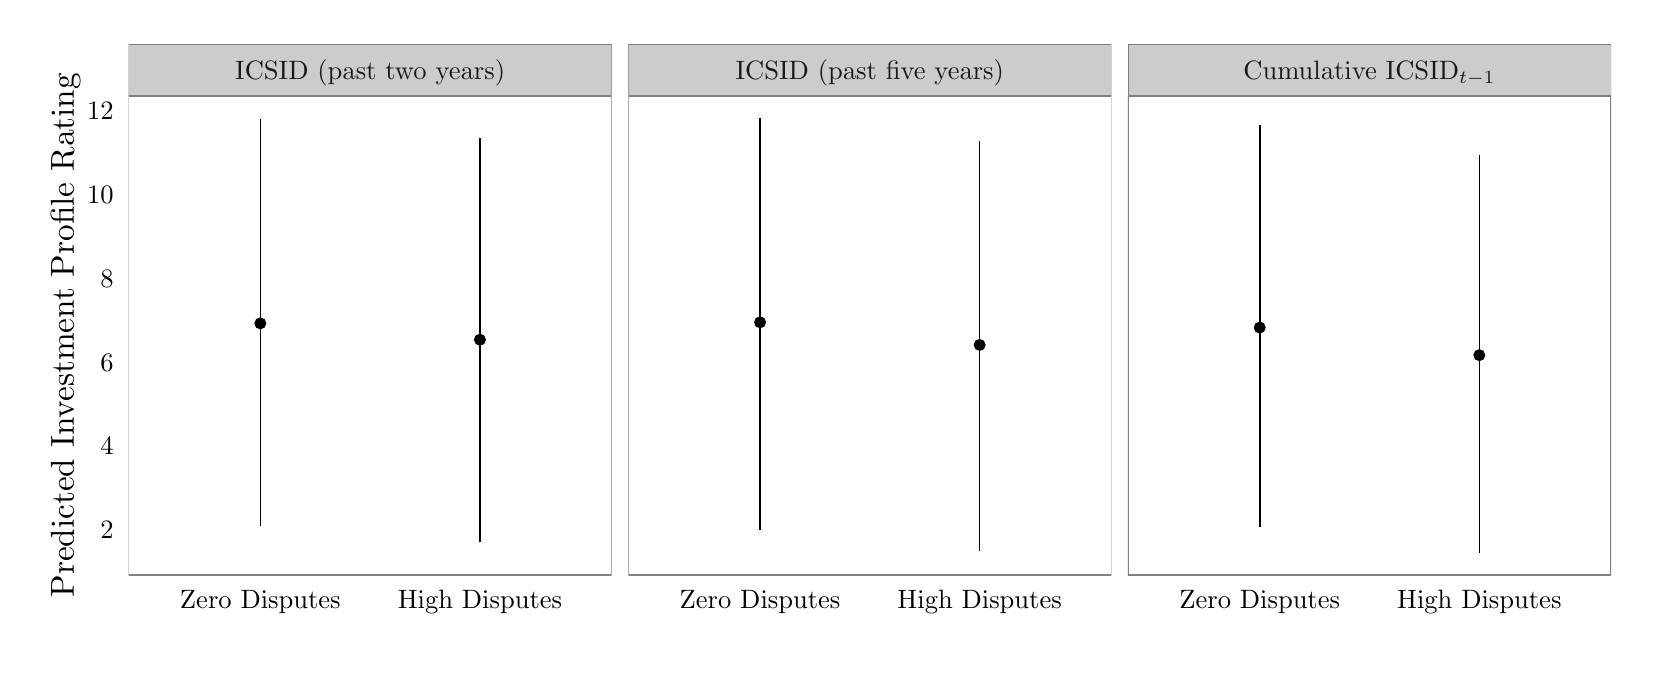
\begin{tikzpicture}[x=1pt,y=1pt]
\definecolor[named]{drawColor}{rgb}{0.00,0.00,0.00}
\definecolor[named]{fillColor}{rgb}{1.00,1.00,1.00}
\fill[color=fillColor,] (0,0) rectangle (578.16,231.26);
\begin{scope}
\path[clip] (  0.00,  0.00) rectangle (578.16,231.26);
\end{scope}
\begin{scope}
\path[clip] (  0.00,  0.00) rectangle (578.16,231.26);
\end{scope}
\begin{scope}
\path[clip] (  0.00,  0.00) rectangle (578.16,231.26);
\end{scope}
\begin{scope}
\path[clip] (  0.00,  0.00) rectangle (578.16,231.26);
\end{scope}
\begin{scope}
\path[clip] (  0.00,  0.00) rectangle (578.16,231.26);
\end{scope}
\begin{scope}
\path[clip] (  0.00,  0.00) rectangle (578.16,231.26);
\end{scope}
\begin{scope}
\path[clip] (  0.00,  0.00) rectangle (578.16,231.26);
\end{scope}
\begin{scope}
\path[clip] (  0.00,  0.00) rectangle (578.16,231.26);
\end{scope}
\begin{scope}
\path[clip] (  0.00,  0.00) rectangle (578.16,231.26);
\end{scope}
\begin{scope}
\path[clip] (  0.00,  0.00) rectangle (578.16,231.26);
\end{scope}
\begin{scope}
\path[clip] (  0.00,  0.00) rectangle (578.16,231.26);
\end{scope}
\begin{scope}
\path[clip] (  0.00,  0.00) rectangle (578.16,231.26);
\end{scope}
\begin{scope}
\path[clip] (  0.00,  0.00) rectangle (578.16,231.26);
\end{scope}
\begin{scope}
\path[clip] (  0.00,  0.00) rectangle (578.16,231.26);
\definecolor[named]{drawColor}{rgb}{1.00,1.00,1.00}
\definecolor[named]{fillColor}{rgb}{1.00,1.00,1.00}

\draw[color=drawColor,line width= 0.6pt,line cap=round,line join=round,fill=fillColor,] (  0.00,  0.00) rectangle (578.16,231.26);
\end{scope}
\begin{scope}
\path[clip] (  0.00,  0.00) rectangle (578.16,231.26);
\end{scope}
\begin{scope}
\path[clip] ( 36.46, 33.48) rectangle (211.03,206.65);
\definecolor[named]{fillColor}{rgb}{1.00,1.00,1.00}

\draw[fill=fillColor,draw opacity=0.00,] ( 36.46, 33.48) rectangle (211.03,206.65);
\definecolor[named]{drawColor}{rgb}{0.00,0.00,0.00}
\definecolor[named]{fillColor}{rgb}{0.00,0.00,0.00}

\draw[color=drawColor,line width= 0.6pt,line join=round,fill=fillColor,] ( 84.07, 51.23) -- ( 84.07,198.22);

\draw[color=drawColor,line width= 0.6pt,line join=round,fill=fillColor,] (163.42, 45.31) -- (163.42,191.56);

\draw[color=drawColor,line width= 0.4pt,line cap=round,line join=round,fill=fillColor,] ( 84.07,124.41) circle (  1.96);

\draw[color=drawColor,line width= 0.4pt,line cap=round,line join=round,fill=fillColor,] (163.42,118.50) circle (  1.96);
\definecolor[named]{drawColor}{rgb}{0.50,0.50,0.50}

\draw[color=drawColor,line width= 0.6pt,line cap=round,line join=round,fill opacity=0.00,] ( 36.46, 33.48) rectangle (211.03,206.65);
\end{scope}
\begin{scope}
\path[clip] (  0.00,  0.00) rectangle (578.16,231.26);
\end{scope}
\begin{scope}
\path[clip] (217.03, 33.48) rectangle (391.59,206.65);
\definecolor[named]{fillColor}{rgb}{1.00,1.00,1.00}

\draw[fill=fillColor,draw opacity=0.00,] (217.03, 33.48) rectangle (391.59,206.65);
\definecolor[named]{drawColor}{rgb}{0.00,0.00,0.00}
\definecolor[named]{fillColor}{rgb}{0.00,0.00,0.00}

\draw[color=drawColor,line width= 0.6pt,line join=round,fill=fillColor,] (264.64, 49.75) -- (264.64,198.78);

\draw[color=drawColor,line width= 0.6pt,line join=round,fill=fillColor,] (343.99, 42.06) -- (343.99,190.16);

\draw[color=drawColor,line width= 0.4pt,line cap=round,line join=round,fill=fillColor,] (264.64,124.79) circle (  1.96);

\draw[color=drawColor,line width= 0.4pt,line cap=round,line join=round,fill=fillColor,] (343.99,116.61) circle (  1.96);
\definecolor[named]{drawColor}{rgb}{0.50,0.50,0.50}

\draw[color=drawColor,line width= 0.6pt,line cap=round,line join=round,fill opacity=0.00,] (217.03, 33.48) rectangle (391.59,206.65);
\end{scope}
\begin{scope}
\path[clip] (  0.00,  0.00) rectangle (578.16,231.26);
\end{scope}
\begin{scope}
\path[clip] (397.59, 33.48) rectangle (572.16,206.65);
\definecolor[named]{fillColor}{rgb}{1.00,1.00,1.00}

\draw[fill=fillColor,draw opacity=0.00,] (397.59, 33.48) rectangle (572.16,206.65);
\definecolor[named]{drawColor}{rgb}{0.00,0.00,0.00}
\definecolor[named]{fillColor}{rgb}{0.00,0.00,0.00}

\draw[color=drawColor,line width= 0.6pt,line join=round,fill=fillColor,] (445.20, 50.70) -- (445.20,196.03);

\draw[color=drawColor,line width= 0.6pt,line join=round,fill=fillColor,] (524.55, 41.35) -- (524.55,185.34);

\draw[color=drawColor,line width= 0.4pt,line cap=round,line join=round,fill=fillColor,] (445.20,122.89) circle (  1.96);

\draw[color=drawColor,line width= 0.4pt,line cap=round,line join=round,fill=fillColor,] (524.55,112.93) circle (  1.96);
\definecolor[named]{drawColor}{rgb}{0.50,0.50,0.50}

\draw[color=drawColor,line width= 0.6pt,line cap=round,line join=round,fill opacity=0.00,] (397.59, 33.48) rectangle (572.16,206.65);
\end{scope}
\begin{scope}
\path[clip] (  0.00,  0.00) rectangle (578.16,231.26);
\end{scope}
\begin{scope}
\path[clip] (  0.00,  0.00) rectangle (578.16,231.26);
\end{scope}
\begin{scope}
\path[clip] (  0.00,  0.00) rectangle (578.16,231.26);
\end{scope}
\begin{scope}
\path[clip] ( 36.46,206.65) rectangle (211.03,225.26);
\definecolor[named]{drawColor}{rgb}{0.50,0.50,0.50}
\definecolor[named]{fillColor}{rgb}{0.80,0.80,0.80}

\draw[color=drawColor,line width= 0.2pt,line cap=round,line join=round,fill=fillColor,] ( 36.46,206.65) rectangle (211.03,225.26);
\definecolor[named]{drawColor}{rgb}{0.10,0.10,0.10}

\node[color=drawColor,anchor=base,inner sep=0pt, outer sep=0pt, scale=  0.96] at (123.75,212.65) {ICSID (past two years)%
};
\end{scope}
\begin{scope}
\path[clip] ( 36.46,206.65) rectangle (211.03,225.26);
\end{scope}
\begin{scope}
\path[clip] (  0.00,  0.00) rectangle (578.16,231.26);
\end{scope}
\begin{scope}
\path[clip] (  0.00,  0.00) rectangle (578.16,231.26);
\end{scope}
\begin{scope}
\path[clip] (  0.00,  0.00) rectangle (578.16,231.26);
\end{scope}
\begin{scope}
\path[clip] (  0.00,  0.00) rectangle (578.16,231.26);
\end{scope}
\begin{scope}
\path[clip] (  0.00,  0.00) rectangle (578.16,231.26);
\end{scope}
\begin{scope}
\path[clip] (  0.00,  0.00) rectangle (578.16,231.26);
\end{scope}
\begin{scope}
\path[clip] (217.03,206.65) rectangle (391.59,225.26);
\definecolor[named]{drawColor}{rgb}{0.50,0.50,0.50}
\definecolor[named]{fillColor}{rgb}{0.80,0.80,0.80}

\draw[color=drawColor,line width= 0.2pt,line cap=round,line join=round,fill=fillColor,] (217.03,206.65) rectangle (391.59,225.26);
\definecolor[named]{drawColor}{rgb}{0.10,0.10,0.10}

\node[color=drawColor,anchor=base,inner sep=0pt, outer sep=0pt, scale=  0.96] at (304.31,212.65) {ICSID (past five years)%
};
\end{scope}
\begin{scope}
\path[clip] (217.03,206.65) rectangle (391.59,225.26);
\end{scope}
\begin{scope}
\path[clip] (  0.00,  0.00) rectangle (578.16,231.26);
\end{scope}
\begin{scope}
\path[clip] (  0.00,  0.00) rectangle (578.16,231.26);
\end{scope}
\begin{scope}
\path[clip] (  0.00,  0.00) rectangle (578.16,231.26);
\end{scope}
\begin{scope}
\path[clip] (  0.00,  0.00) rectangle (578.16,231.26);
\end{scope}
\begin{scope}
\path[clip] (  0.00,  0.00) rectangle (578.16,231.26);
\end{scope}
\begin{scope}
\path[clip] (  0.00,  0.00) rectangle (578.16,231.26);
\end{scope}
\begin{scope}
\path[clip] (397.59,206.65) rectangle (572.16,225.26);
\definecolor[named]{drawColor}{rgb}{0.50,0.50,0.50}
\definecolor[named]{fillColor}{rgb}{0.80,0.80,0.80}

\draw[color=drawColor,line width= 0.2pt,line cap=round,line join=round,fill=fillColor,] (397.59,206.65) rectangle (572.16,225.26);
\definecolor[named]{drawColor}{rgb}{0.10,0.10,0.10}

\node[color=drawColor,anchor=base,inner sep=0pt, outer sep=0pt, scale=  0.96] at (484.88,212.65) {Cumulative ICSID$_{t-1}$%
};
\end{scope}
\begin{scope}
\path[clip] (397.59,206.65) rectangle (572.16,225.26);
\end{scope}
\begin{scope}
\path[clip] (  0.00,  0.00) rectangle (578.16,231.26);
\end{scope}
\begin{scope}
\path[clip] (  0.00,  0.00) rectangle (578.16,231.26);
\end{scope}
\begin{scope}
\path[clip] (  0.00,  0.00) rectangle (578.16,231.26);
\end{scope}
\begin{scope}
\path[clip] (  0.00,  0.00) rectangle (578.16,231.26);
\end{scope}
\begin{scope}
\path[clip] (  0.00,  0.00) rectangle (578.16,231.26);
\end{scope}
\begin{scope}
\path[clip] (  0.00,  0.00) rectangle (578.16,231.26);
\end{scope}
\begin{scope}
\path[clip] (  0.00,  0.00) rectangle (578.16,231.26);
\end{scope}
\begin{scope}
\path[clip] (  0.00,  0.00) rectangle (578.16,231.26);
\end{scope}
\begin{scope}
\path[clip] (  0.00,  0.00) rectangle (578.16,231.26);
\definecolor[named]{drawColor}{rgb}{0.00,0.00,0.00}

\node[color=drawColor,anchor=base east,inner sep=0pt, outer sep=0pt, scale=  0.96] at ( 31.06, 46.57) {2%
};

\node[color=drawColor,anchor=base east,inner sep=0pt, outer sep=0pt, scale=  0.96] at ( 31.06, 76.85) {4%
};

\node[color=drawColor,anchor=base east,inner sep=0pt, outer sep=0pt, scale=  0.96] at ( 31.06,107.14) {6%
};

\node[color=drawColor,anchor=base east,inner sep=0pt, outer sep=0pt, scale=  0.96] at ( 31.06,137.42) {8%
};

\node[color=drawColor,anchor=base east,inner sep=0pt, outer sep=0pt, scale=  0.96] at ( 31.06,167.70) {10%
};

\node[color=drawColor,anchor=base east,inner sep=0pt, outer sep=0pt, scale=  0.96] at ( 31.06,197.98) {12%
};
\end{scope}
\begin{scope}
\path[clip] (  0.00,  0.00) rectangle (578.16,231.26);
\end{scope}
\begin{scope}
\path[clip] (  0.00,  0.00) rectangle (578.16,231.26);
\end{scope}
\begin{scope}
\path[clip] (  0.00,  0.00) rectangle (578.16,231.26);
\end{scope}
\begin{scope}
\path[clip] (  0.00,  0.00) rectangle (578.16,231.26);
\end{scope}
\begin{scope}
\path[clip] (  0.00,  0.00) rectangle (578.16,231.26);
\end{scope}
\begin{scope}
\path[clip] (  0.00,  0.00) rectangle (578.16,231.26);
\end{scope}
\begin{scope}
\path[clip] (  0.00,  0.00) rectangle (578.16,231.26);
\end{scope}
\begin{scope}
\path[clip] (  0.00,  0.00) rectangle (578.16,231.26);
\end{scope}
\begin{scope}
\path[clip] (  0.00,  0.00) rectangle (578.16,231.26);
\end{scope}
\begin{scope}
\path[clip] (  0.00,  0.00) rectangle (578.16,231.26);
\end{scope}
\begin{scope}
\path[clip] (  0.00,  0.00) rectangle (578.16,231.26);
\end{scope}
\begin{scope}
\path[clip] (  0.00,  0.00) rectangle (578.16,231.26);
\end{scope}
\begin{scope}
\path[clip] (  0.00,  0.00) rectangle (578.16,231.26);
\end{scope}
\begin{scope}
\path[clip] (  0.00,  0.00) rectangle (578.16,231.26);
\end{scope}
\begin{scope}
\path[clip] (  0.00,  0.00) rectangle (578.16,231.26);
\end{scope}
\begin{scope}
\path[clip] (  0.00,  0.00) rectangle (578.16,231.26);
\end{scope}
\begin{scope}
\path[clip] (  0.00,  0.00) rectangle (578.16,231.26);
\end{scope}
\begin{scope}
\path[clip] (  0.00,  0.00) rectangle (578.16,231.26);
\definecolor[named]{drawColor}{rgb}{0.00,0.00,0.00}

\node[color=drawColor,anchor=base,inner sep=0pt, outer sep=0pt, scale=  0.96] at ( 84.07, 21.46) {Zero Disputes%
};

\node[color=drawColor,anchor=base,inner sep=0pt, outer sep=0pt, scale=  0.96] at (163.42, 21.46) {High Disputes%
};
\end{scope}
\begin{scope}
\path[clip] (  0.00,  0.00) rectangle (578.16,231.26);
\end{scope}
\begin{scope}
\path[clip] (  0.00,  0.00) rectangle (578.16,231.26);
\end{scope}
\begin{scope}
\path[clip] (  0.00,  0.00) rectangle (578.16,231.26);
\end{scope}
\begin{scope}
\path[clip] (  0.00,  0.00) rectangle (578.16,231.26);
\end{scope}
\begin{scope}
\path[clip] (  0.00,  0.00) rectangle (578.16,231.26);
\end{scope}
\begin{scope}
\path[clip] (  0.00,  0.00) rectangle (578.16,231.26);
\end{scope}
\begin{scope}
\path[clip] (  0.00,  0.00) rectangle (578.16,231.26);
\end{scope}
\begin{scope}
\path[clip] (  0.00,  0.00) rectangle (578.16,231.26);
\end{scope}
\begin{scope}
\path[clip] (  0.00,  0.00) rectangle (578.16,231.26);
\end{scope}
\begin{scope}
\path[clip] (  0.00,  0.00) rectangle (578.16,231.26);
\end{scope}
\begin{scope}
\path[clip] (  0.00,  0.00) rectangle (578.16,231.26);
\end{scope}
\begin{scope}
\path[clip] (  0.00,  0.00) rectangle (578.16,231.26);
\definecolor[named]{drawColor}{rgb}{0.00,0.00,0.00}

\node[color=drawColor,anchor=base,inner sep=0pt, outer sep=0pt, scale=  0.96] at (264.64, 21.46) {Zero Disputes%
};

\node[color=drawColor,anchor=base,inner sep=0pt, outer sep=0pt, scale=  0.96] at (343.99, 21.46) {High Disputes%
};
\end{scope}
\begin{scope}
\path[clip] (  0.00,  0.00) rectangle (578.16,231.26);
\end{scope}
\begin{scope}
\path[clip] (  0.00,  0.00) rectangle (578.16,231.26);
\end{scope}
\begin{scope}
\path[clip] (  0.00,  0.00) rectangle (578.16,231.26);
\end{scope}
\begin{scope}
\path[clip] (  0.00,  0.00) rectangle (578.16,231.26);
\end{scope}
\begin{scope}
\path[clip] (  0.00,  0.00) rectangle (578.16,231.26);
\end{scope}
\begin{scope}
\path[clip] (  0.00,  0.00) rectangle (578.16,231.26);
\end{scope}
\begin{scope}
\path[clip] (  0.00,  0.00) rectangle (578.16,231.26);
\end{scope}
\begin{scope}
\path[clip] (  0.00,  0.00) rectangle (578.16,231.26);
\end{scope}
\begin{scope}
\path[clip] (  0.00,  0.00) rectangle (578.16,231.26);
\end{scope}
\begin{scope}
\path[clip] (  0.00,  0.00) rectangle (578.16,231.26);
\end{scope}
\begin{scope}
\path[clip] (  0.00,  0.00) rectangle (578.16,231.26);
\end{scope}
\begin{scope}
\path[clip] (  0.00,  0.00) rectangle (578.16,231.26);
\definecolor[named]{drawColor}{rgb}{0.00,0.00,0.00}

\node[color=drawColor,anchor=base,inner sep=0pt, outer sep=0pt, scale=  0.96] at (445.20, 21.46) {Zero Disputes%
};

\node[color=drawColor,anchor=base,inner sep=0pt, outer sep=0pt, scale=  0.96] at (524.55, 21.46) {High Disputes%
};
\end{scope}
\begin{scope}
\path[clip] (  0.00,  0.00) rectangle (578.16,231.26);
\end{scope}
\begin{scope}
\path[clip] (  0.00,  0.00) rectangle (578.16,231.26);
\end{scope}
\begin{scope}
\path[clip] (  0.00,  0.00) rectangle (578.16,231.26);
\end{scope}
\begin{scope}
\path[clip] (  0.00,  0.00) rectangle (578.16,231.26);
\end{scope}
\begin{scope}
\path[clip] (  0.00,  0.00) rectangle (578.16,231.26);
\end{scope}
\begin{scope}
\path[clip] (  0.00,  0.00) rectangle (578.16,231.26);
\end{scope}
\begin{scope}
\path[clip] (  0.00,  0.00) rectangle (578.16,231.26);
\end{scope}
\begin{scope}
\path[clip] (  0.00,  0.00) rectangle (578.16,231.26);
\end{scope}
\begin{scope}
\path[clip] (  0.00,  0.00) rectangle (578.16,231.26);
\definecolor[named]{drawColor}{rgb}{0.00,0.00,0.00}

\node[rotate= 90.00,color=drawColor,anchor=base,inner sep=0pt, outer sep=0pt, scale=  1.20] at ( 16.66,120.06) {Predicted Investment Profile Rating%
};
\end{scope}
\begin{scope}
\path[clip] (  0.00,  0.00) rectangle (578.16,231.26);
\end{scope}
\begin{scope}
\path[clip] (  0.00,  0.00) rectangle (578.16,231.26);
\end{scope}
\begin{scope}
\path[clip] (  0.00,  0.00) rectangle (578.16,231.26);
\end{scope}
\begin{scope}
\path[clip] (  0.00,  0.00) rectangle (578.16,231.26);
\end{scope}
\begin{scope}
\path[clip] (  0.00,  0.00) rectangle (578.16,231.26);
\end{scope}
\end{tikzpicture}
}
	\caption*{Note: Here we show a typical country's predicted rating on investment profile under a scenario where a country faces a minimum versus the 99$^{th}$ percentile number of ICSID disputes. Results were obtained by using simulations that accounted for inferential uncertainty. The point estimates here represent the mean predicted ratings and the line represents the 95\% level of uncertainty associated with these estimates.}
\end{figure}
\FloatBarrier

% \newpage

The fact that the level of uncertainty around our predicted values is so high, however, raises an interesting question about the impact of the passage of time. Developing a system of effective monitoring and enforcement is likely to take time as does reputational change. Much of the literature on investment treaties, however, assumes that dispute involvement entails costs, regardless of time period. This is an unnecessary assumption that we examine more closely by unpacking potential temporal variation in the effect that ICSID disputes have on a country's reputation.

\begin{figure}[ht]
	\centering
	\caption{Change in Effect of ICSID Disputes Over Time}
	\label{fig:dispEffectYear}
	\resizebox{1\textwidth}{!}{% Created by tikzDevice version 0.7.0 on 2015-01-23 00:08:45
% !TEX encoding = UTF-8 Unicode
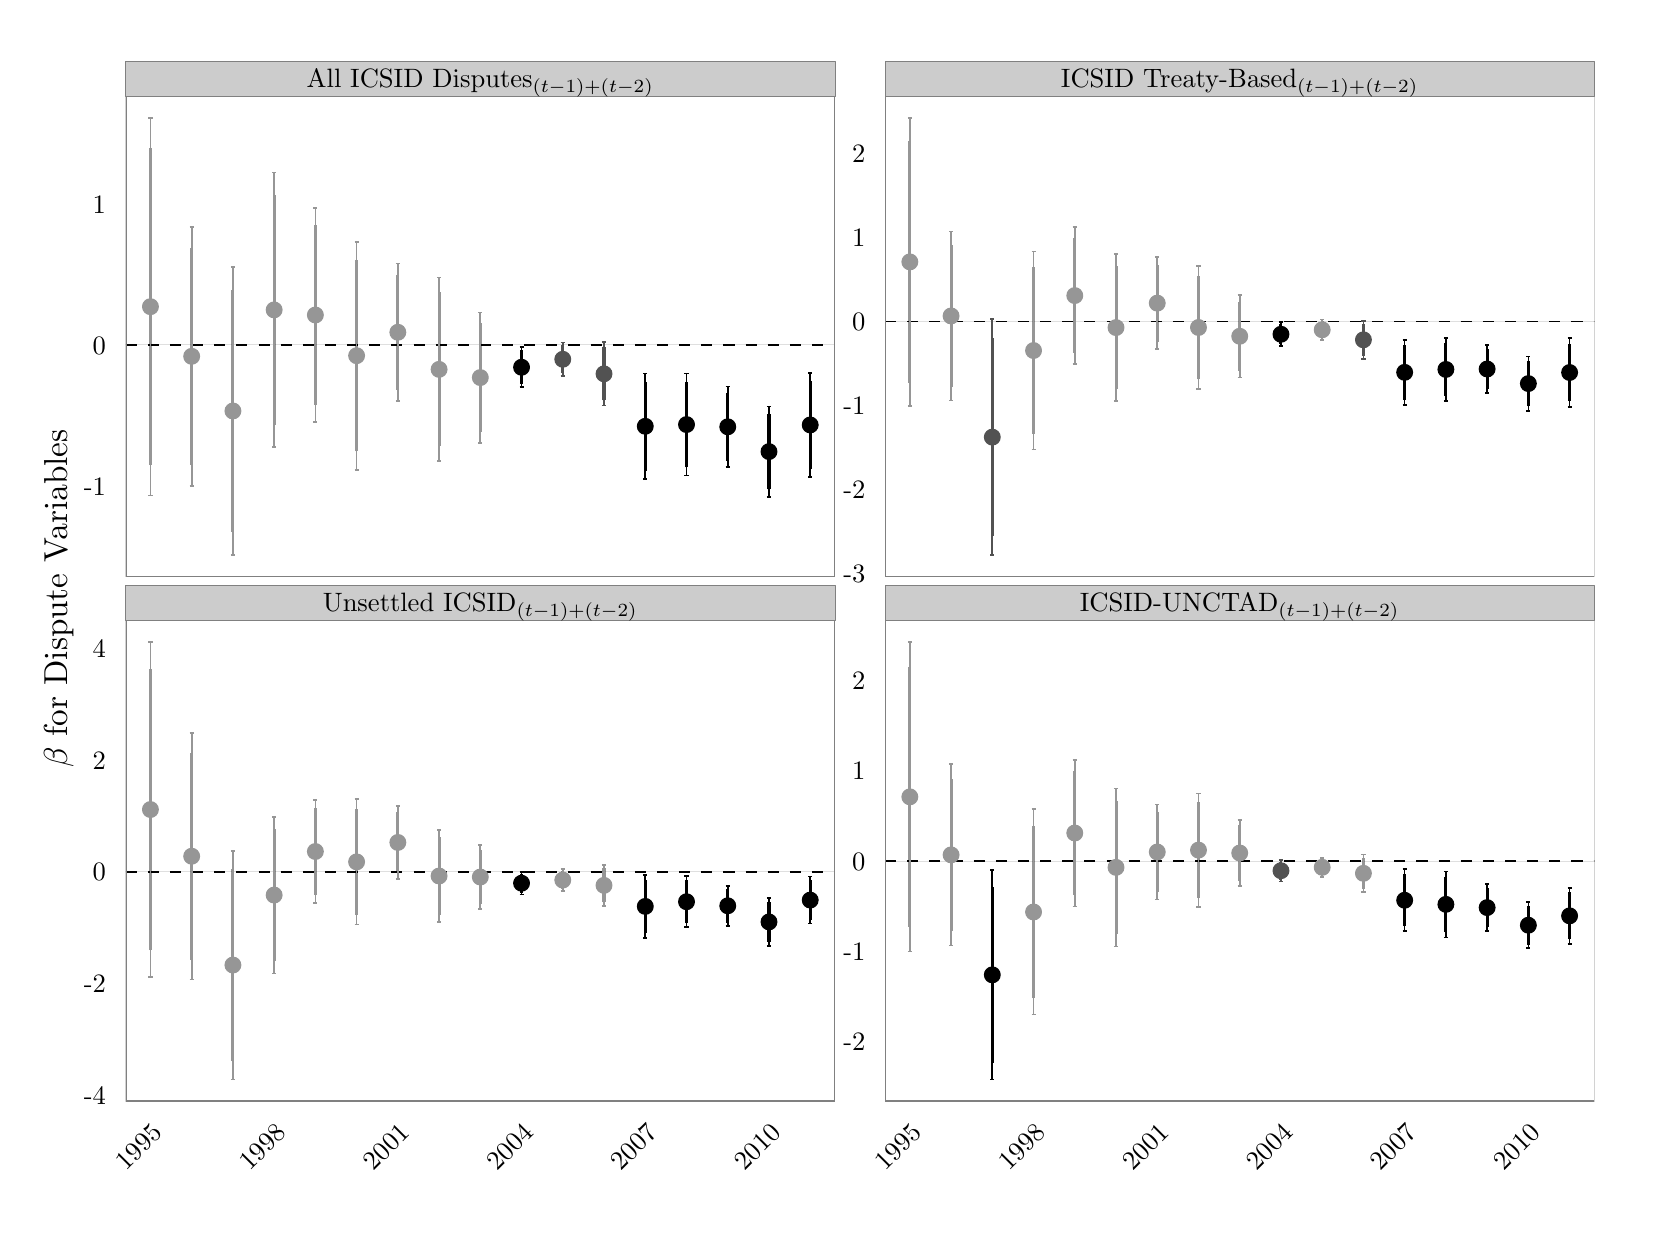
\begin{tikzpicture}[x=1pt,y=1pt]
\definecolor[named]{fillColor}{rgb}{1.00,1.00,1.00}
\path[use as bounding box,fill=fillColor,fill opacity=0.00] (0,0) rectangle (578.16,433.62);
\begin{scope}
\path[clip] (  0.00,  0.00) rectangle (578.16,433.62);
\definecolor[named]{drawColor}{rgb}{1.00,1.00,1.00}
\definecolor[named]{fillColor}{rgb}{1.00,1.00,1.00}

\path[draw=drawColor,line width= 0.6pt,line join=round,line cap=round,fill=fillColor] (  0.00,  0.00) rectangle (578.16,433.62);
\end{scope}
\begin{scope}
\path[clip] ( 35.42,235.13) rectangle (291.71,408.94);
\definecolor[named]{fillColor}{rgb}{1.00,1.00,1.00}

\path[fill=fillColor] ( 35.42,235.13) rectangle (291.71,408.94);
\definecolor[named]{drawColor}{rgb}{0.59,0.59,0.59}
\definecolor[named]{fillColor}{rgb}{0.59,0.59,0.59}

\path[draw=drawColor,draw opacity=0.30,line width= 0.3pt,line join=round,fill=fillColor,fill opacity=0.30] ( 44.36,264.57) -- ( 44.36,401.04);

\path[draw=drawColor,draw opacity=0.30,line width= 0.3pt,line join=round,fill=fillColor,fill opacity=0.30] ( 59.26,268.08) -- ( 59.26,361.64);

\path[draw=drawColor,draw opacity=0.30,line width= 0.3pt,line join=round,fill=fillColor,fill opacity=0.30] ( 74.16,243.03) -- ( 74.16,347.20);

\path[draw=drawColor,draw opacity=0.30,line width= 0.3pt,line join=round,fill=fillColor,fill opacity=0.30] ( 89.06,282.03) -- ( 89.06,381.24);

\path[draw=drawColor,draw opacity=0.30,line width= 0.3pt,line join=round,fill=fillColor,fill opacity=0.30] (103.96,291.12) -- (103.96,368.46);

\path[draw=drawColor,draw opacity=0.30,line width= 0.3pt,line join=round,fill=fillColor,fill opacity=0.30] (118.86,273.90) -- (118.86,356.28);

\path[draw=drawColor,draw opacity=0.30,line width= 0.3pt,line join=round,fill=fillColor,fill opacity=0.30] (133.76,298.70) -- (133.76,348.40);

\path[draw=drawColor,draw opacity=0.30,line width= 0.3pt,line join=round,fill=fillColor,fill opacity=0.30] (148.66,276.98) -- (148.66,343.29);

\path[draw=drawColor,draw opacity=0.30,line width= 0.3pt,line join=round,fill=fillColor,fill opacity=0.30] (163.56,283.63) -- (163.56,330.74);
\definecolor[named]{drawColor}{rgb}{0.00,0.00,0.00}
\definecolor[named]{fillColor}{rgb}{0.00,0.00,0.00}

\path[draw=drawColor,draw opacity=0.30,line width= 0.3pt,line join=round,fill=fillColor,fill opacity=0.30] (178.46,303.67) -- (178.46,318.14);
\definecolor[named]{drawColor}{rgb}{0.32,0.32,0.32}
\definecolor[named]{fillColor}{rgb}{0.32,0.32,0.32}

\path[draw=drawColor,draw opacity=0.30,line width= 0.3pt,line join=round,fill=fillColor,fill opacity=0.30] (193.36,307.68) -- (193.36,319.90);

\path[draw=drawColor,draw opacity=0.30,line width= 0.3pt,line join=round,fill=fillColor,fill opacity=0.30] (208.26,297.13) -- (208.26,319.93);
\definecolor[named]{drawColor}{rgb}{0.00,0.00,0.00}
\definecolor[named]{fillColor}{rgb}{0.00,0.00,0.00}

\path[draw=drawColor,draw opacity=0.30,line width= 0.3pt,line join=round,fill=fillColor,fill opacity=0.30] (223.17,270.42) -- (223.17,308.71);

\path[draw=drawColor,draw opacity=0.30,line width= 0.3pt,line join=round,fill=fillColor,fill opacity=0.30] (238.07,271.74) -- (238.07,308.67);

\path[draw=drawColor,draw opacity=0.30,line width= 0.3pt,line join=round,fill=fillColor,fill opacity=0.30] (252.97,274.84) -- (252.97,303.93);

\path[draw=drawColor,draw opacity=0.30,line width= 0.3pt,line join=round,fill=fillColor,fill opacity=0.30] (267.87,264.12) -- (267.87,296.74);

\path[draw=drawColor,draw opacity=0.30,line width= 0.3pt,line join=round,fill=fillColor,fill opacity=0.30] (282.77,271.21) -- (282.77,308.92);
\definecolor[named]{drawColor}{rgb}{0.59,0.59,0.59}
\definecolor[named]{fillColor}{rgb}{0.59,0.59,0.59}

\path[draw=drawColor,line width= 1.1pt,line join=round,fill=fillColor] ( 44.36,275.54) -- ( 44.36,390.07);

\path[draw=drawColor,line width= 1.1pt,line join=round,fill=fillColor] ( 59.26,275.60) -- ( 59.26,354.12);

\path[draw=drawColor,line width= 1.1pt,line join=round,fill=fillColor] ( 74.16,251.40) -- ( 74.16,338.82);

\path[draw=drawColor,line width= 1.1pt,line join=round,fill=fillColor] ( 89.06,290.00) -- ( 89.06,373.26);

\path[draw=drawColor,line width= 1.1pt,line join=round,fill=fillColor] (103.96,297.34) -- (103.96,362.24);

\path[draw=drawColor,line width= 1.1pt,line join=round,fill=fillColor] (118.86,280.52) -- (118.86,349.65);

\path[draw=drawColor,line width= 1.1pt,line join=round,fill=fillColor] (133.76,302.70) -- (133.76,344.41);

\path[draw=drawColor,line width= 1.1pt,line join=round,fill=fillColor] (148.66,282.31) -- (148.66,337.96);

\path[draw=drawColor,line width= 1.1pt,line join=round,fill=fillColor] (163.56,287.42) -- (163.56,326.95);
\definecolor[named]{drawColor}{rgb}{0.00,0.00,0.00}
\definecolor[named]{fillColor}{rgb}{0.00,0.00,0.00}

\path[draw=drawColor,line width= 1.1pt,line join=round,fill=fillColor] (178.46,304.83) -- (178.46,316.98);
\definecolor[named]{drawColor}{rgb}{0.32,0.32,0.32}
\definecolor[named]{fillColor}{rgb}{0.32,0.32,0.32}

\path[draw=drawColor,line width= 1.1pt,line join=round,fill=fillColor] (193.36,308.66) -- (193.36,318.92);

\path[draw=drawColor,line width= 1.1pt,line join=round,fill=fillColor] (208.26,298.97) -- (208.26,318.10);
\definecolor[named]{drawColor}{rgb}{0.00,0.00,0.00}
\definecolor[named]{fillColor}{rgb}{0.00,0.00,0.00}

\path[draw=drawColor,line width= 1.1pt,line join=round,fill=fillColor] (223.17,273.50) -- (223.17,305.63);

\path[draw=drawColor,line width= 1.1pt,line join=round,fill=fillColor] (238.07,274.71) -- (238.07,305.70);

\path[draw=drawColor,line width= 1.1pt,line join=round,fill=fillColor] (252.97,277.18) -- (252.97,301.59);

\path[draw=drawColor,line width= 1.1pt,line join=round,fill=fillColor] (267.87,266.74) -- (267.87,294.12);

\path[draw=drawColor,line width= 1.1pt,line join=round,fill=fillColor] (282.77,274.24) -- (282.77,305.89);

\path[draw=drawColor,line width= 0.6pt,dash pattern=on 4pt off 4pt ,line join=round,fill=fillColor] ( 35.42,318.97) -- (291.71,318.97);
\definecolor[named]{drawColor}{rgb}{0.59,0.59,0.59}
\definecolor[named]{fillColor}{rgb}{0.59,0.59,0.59}

\path[draw=drawColor,line width= 0.4pt,line join=round,line cap=round,fill=fillColor] ( 44.36,332.80) circle (  2.85);

\path[draw=drawColor,line width= 0.4pt,line join=round,line cap=round,fill=fillColor] ( 59.26,314.86) circle (  2.85);

\path[draw=drawColor,line width= 0.4pt,line join=round,line cap=round,fill=fillColor] ( 74.16,295.11) circle (  2.85);

\path[draw=drawColor,line width= 0.4pt,line join=round,line cap=round,fill=fillColor] ( 89.06,331.63) circle (  2.85);

\path[draw=drawColor,line width= 0.4pt,line join=round,line cap=round,fill=fillColor] (103.96,329.79) circle (  2.85);

\path[draw=drawColor,line width= 0.4pt,line join=round,line cap=round,fill=fillColor] (118.86,315.09) circle (  2.85);

\path[draw=drawColor,line width= 0.4pt,line join=round,line cap=round,fill=fillColor] (133.76,323.55) circle (  2.85);

\path[draw=drawColor,line width= 0.4pt,line join=round,line cap=round,fill=fillColor] (148.66,310.14) circle (  2.85);

\path[draw=drawColor,line width= 0.4pt,line join=round,line cap=round,fill=fillColor] (163.56,307.18) circle (  2.85);
\definecolor[named]{drawColor}{rgb}{0.00,0.00,0.00}
\definecolor[named]{fillColor}{rgb}{0.00,0.00,0.00}

\path[draw=drawColor,line width= 0.4pt,line join=round,line cap=round,fill=fillColor] (178.46,310.91) circle (  2.85);
\definecolor[named]{drawColor}{rgb}{0.32,0.32,0.32}
\definecolor[named]{fillColor}{rgb}{0.32,0.32,0.32}

\path[draw=drawColor,line width= 0.4pt,line join=round,line cap=round,fill=fillColor] (193.36,313.79) circle (  2.85);

\path[draw=drawColor,line width= 0.4pt,line join=round,line cap=round,fill=fillColor] (208.26,308.53) circle (  2.85);
\definecolor[named]{drawColor}{rgb}{0.00,0.00,0.00}
\definecolor[named]{fillColor}{rgb}{0.00,0.00,0.00}

\path[draw=drawColor,line width= 0.4pt,line join=round,line cap=round,fill=fillColor] (223.17,289.57) circle (  2.85);

\path[draw=drawColor,line width= 0.4pt,line join=round,line cap=round,fill=fillColor] (238.07,290.20) circle (  2.85);

\path[draw=drawColor,line width= 0.4pt,line join=round,line cap=round,fill=fillColor] (252.97,289.39) circle (  2.85);

\path[draw=drawColor,line width= 0.4pt,line join=round,line cap=round,fill=fillColor] (267.87,280.43) circle (  2.85);

\path[draw=drawColor,line width= 0.4pt,line join=round,line cap=round,fill=fillColor] (282.77,290.06) circle (  2.85);
\definecolor[named]{drawColor}{rgb}{0.59,0.59,0.59}

\path[draw=drawColor,line width= 0.6pt,line join=round] ( 43.62,401.04) --
	( 45.11,401.04);

\path[draw=drawColor,line width= 0.6pt,line join=round] ( 44.36,401.04) --
	( 44.36,264.57);

\path[draw=drawColor,line width= 0.6pt,line join=round] ( 43.62,264.57) --
	( 45.11,264.57);

\path[draw=drawColor,line width= 0.6pt,line join=round] ( 58.52,361.64) --
	( 60.01,361.64);

\path[draw=drawColor,line width= 0.6pt,line join=round] ( 59.26,361.64) --
	( 59.26,268.08);

\path[draw=drawColor,line width= 0.6pt,line join=round] ( 58.52,268.08) --
	( 60.01,268.08);

\path[draw=drawColor,line width= 0.6pt,line join=round] ( 73.42,347.20) --
	( 74.91,347.20);

\path[draw=drawColor,line width= 0.6pt,line join=round] ( 74.16,347.20) --
	( 74.16,243.03);

\path[draw=drawColor,line width= 0.6pt,line join=round] ( 73.42,243.03) --
	( 74.91,243.03);

\path[draw=drawColor,line width= 0.6pt,line join=round] ( 88.32,381.24) --
	( 89.81,381.24);

\path[draw=drawColor,line width= 0.6pt,line join=round] ( 89.06,381.24) --
	( 89.06,282.03);

\path[draw=drawColor,line width= 0.6pt,line join=round] ( 88.32,282.03) --
	( 89.81,282.03);

\path[draw=drawColor,line width= 0.6pt,line join=round] (103.22,368.46) --
	(104.71,368.46);

\path[draw=drawColor,line width= 0.6pt,line join=round] (103.96,368.46) --
	(103.96,291.12);

\path[draw=drawColor,line width= 0.6pt,line join=round] (103.22,291.12) --
	(104.71,291.12);

\path[draw=drawColor,line width= 0.6pt,line join=round] (118.12,356.28) --
	(119.61,356.28);

\path[draw=drawColor,line width= 0.6pt,line join=round] (118.86,356.28) --
	(118.86,273.90);

\path[draw=drawColor,line width= 0.6pt,line join=round] (118.12,273.90) --
	(119.61,273.90);

\path[draw=drawColor,line width= 0.6pt,line join=round] (133.02,348.40) --
	(134.51,348.40);

\path[draw=drawColor,line width= 0.6pt,line join=round] (133.76,348.40) --
	(133.76,298.70);

\path[draw=drawColor,line width= 0.6pt,line join=round] (133.02,298.70) --
	(134.51,298.70);

\path[draw=drawColor,line width= 0.6pt,line join=round] (147.92,343.29) --
	(149.41,343.29);

\path[draw=drawColor,line width= 0.6pt,line join=round] (148.66,343.29) --
	(148.66,276.98);

\path[draw=drawColor,line width= 0.6pt,line join=round] (147.92,276.98) --
	(149.41,276.98);

\path[draw=drawColor,line width= 0.6pt,line join=round] (162.82,330.74) --
	(164.31,330.74);

\path[draw=drawColor,line width= 0.6pt,line join=round] (163.56,330.74) --
	(163.56,283.63);

\path[draw=drawColor,line width= 0.6pt,line join=round] (162.82,283.63) --
	(164.31,283.63);
\definecolor[named]{drawColor}{rgb}{0.00,0.00,0.00}

\path[draw=drawColor,line width= 0.6pt,line join=round] (177.72,318.14) --
	(179.21,318.14);

\path[draw=drawColor,line width= 0.6pt,line join=round] (178.46,318.14) --
	(178.46,303.67);

\path[draw=drawColor,line width= 0.6pt,line join=round] (177.72,303.67) --
	(179.21,303.67);
\definecolor[named]{drawColor}{rgb}{0.32,0.32,0.32}

\path[draw=drawColor,line width= 0.6pt,line join=round] (192.62,319.90) --
	(194.11,319.90);

\path[draw=drawColor,line width= 0.6pt,line join=round] (193.36,319.90) --
	(193.36,307.68);

\path[draw=drawColor,line width= 0.6pt,line join=round] (192.62,307.68) --
	(194.11,307.68);

\path[draw=drawColor,line width= 0.6pt,line join=round] (207.52,319.93) --
	(209.01,319.93);

\path[draw=drawColor,line width= 0.6pt,line join=round] (208.26,319.93) --
	(208.26,297.13);

\path[draw=drawColor,line width= 0.6pt,line join=round] (207.52,297.13) --
	(209.01,297.13);
\definecolor[named]{drawColor}{rgb}{0.00,0.00,0.00}

\path[draw=drawColor,line width= 0.6pt,line join=round] (222.42,308.71) --
	(223.91,308.71);

\path[draw=drawColor,line width= 0.6pt,line join=round] (223.17,308.71) --
	(223.17,270.42);

\path[draw=drawColor,line width= 0.6pt,line join=round] (222.42,270.42) --
	(223.91,270.42);

\path[draw=drawColor,line width= 0.6pt,line join=round] (237.32,308.67) --
	(238.81,308.67);

\path[draw=drawColor,line width= 0.6pt,line join=round] (238.07,308.67) --
	(238.07,271.74);

\path[draw=drawColor,line width= 0.6pt,line join=round] (237.32,271.74) --
	(238.81,271.74);

\path[draw=drawColor,line width= 0.6pt,line join=round] (252.22,303.93) --
	(253.71,303.93);

\path[draw=drawColor,line width= 0.6pt,line join=round] (252.97,303.93) --
	(252.97,274.84);

\path[draw=drawColor,line width= 0.6pt,line join=round] (252.22,274.84) --
	(253.71,274.84);

\path[draw=drawColor,line width= 0.6pt,line join=round] (267.12,296.74) --
	(268.61,296.74);

\path[draw=drawColor,line width= 0.6pt,line join=round] (267.87,296.74) --
	(267.87,264.12);

\path[draw=drawColor,line width= 0.6pt,line join=round] (267.12,264.12) --
	(268.61,264.12);

\path[draw=drawColor,line width= 0.6pt,line join=round] (282.02,308.92) --
	(283.51,308.92);

\path[draw=drawColor,line width= 0.6pt,line join=round] (282.77,308.92) --
	(282.77,271.21);

\path[draw=drawColor,line width= 0.6pt,line join=round] (282.02,271.21) --
	(283.51,271.21);
\definecolor[named]{drawColor}{rgb}{0.50,0.50,0.50}

\path[draw=drawColor,line width= 0.6pt,line join=round,line cap=round] ( 35.42,235.13) rectangle (291.71,408.94);
\end{scope}
\begin{scope}
\path[clip] (309.83,235.13) rectangle (566.12,408.94);
\definecolor[named]{fillColor}{rgb}{1.00,1.00,1.00}

\path[fill=fillColor] (309.83,235.13) rectangle (566.12,408.94);
\definecolor[named]{drawColor}{rgb}{0.59,0.59,0.59}
\definecolor[named]{fillColor}{rgb}{0.59,0.59,0.59}

\path[draw=drawColor,draw opacity=0.30,line width= 0.3pt,line join=round,fill=fillColor,fill opacity=0.30] (318.77,296.91) -- (318.77,401.04);

\path[draw=drawColor,draw opacity=0.30,line width= 0.3pt,line join=round,fill=fillColor,fill opacity=0.30] (333.67,298.91) -- (333.67,359.98);
\definecolor[named]{drawColor}{rgb}{0.32,0.32,0.32}
\definecolor[named]{fillColor}{rgb}{0.32,0.32,0.32}

\path[draw=drawColor,draw opacity=0.30,line width= 0.3pt,line join=round,fill=fillColor,fill opacity=0.30] (348.57,243.03) -- (348.57,328.29);
\definecolor[named]{drawColor}{rgb}{0.59,0.59,0.59}
\definecolor[named]{fillColor}{rgb}{0.59,0.59,0.59}

\path[draw=drawColor,draw opacity=0.30,line width= 0.3pt,line join=round,fill=fillColor,fill opacity=0.30] (363.47,281.18) -- (363.47,352.72);

\path[draw=drawColor,draw opacity=0.30,line width= 0.3pt,line join=round,fill=fillColor,fill opacity=0.30] (378.37,312.13) -- (378.37,361.49);

\path[draw=drawColor,draw opacity=0.30,line width= 0.3pt,line join=round,fill=fillColor,fill opacity=0.30] (393.27,298.64) -- (393.27,351.85);

\path[draw=drawColor,draw opacity=0.30,line width= 0.3pt,line join=round,fill=fillColor,fill opacity=0.30] (408.17,317.52) -- (408.17,350.65);

\path[draw=drawColor,draw opacity=0.30,line width= 0.3pt,line join=round,fill=fillColor,fill opacity=0.30] (423.07,302.98) -- (423.07,347.58);

\path[draw=drawColor,draw opacity=0.30,line width= 0.3pt,line join=round,fill=fillColor,fill opacity=0.30] (437.97,307.17) -- (437.97,337.03);
\definecolor[named]{drawColor}{rgb}{0.00,0.00,0.00}
\definecolor[named]{fillColor}{rgb}{0.00,0.00,0.00}

\path[draw=drawColor,draw opacity=0.30,line width= 0.3pt,line join=round,fill=fillColor,fill opacity=0.30] (452.87,318.49) -- (452.87,327.17);
\definecolor[named]{drawColor}{rgb}{0.59,0.59,0.59}
\definecolor[named]{fillColor}{rgb}{0.59,0.59,0.59}

\path[draw=drawColor,draw opacity=0.30,line width= 0.3pt,line join=round,fill=fillColor,fill opacity=0.30] (467.77,320.78) -- (467.77,328.11);
\definecolor[named]{drawColor}{rgb}{0.32,0.32,0.32}
\definecolor[named]{fillColor}{rgb}{0.32,0.32,0.32}

\path[draw=drawColor,draw opacity=0.30,line width= 0.3pt,line join=round,fill=fillColor,fill opacity=0.30] (482.67,313.93) -- (482.67,327.71);
\definecolor[named]{drawColor}{rgb}{0.00,0.00,0.00}
\definecolor[named]{fillColor}{rgb}{0.00,0.00,0.00}

\path[draw=drawColor,draw opacity=0.30,line width= 0.3pt,line join=round,fill=fillColor,fill opacity=0.30] (497.57,297.29) -- (497.57,320.85);

\path[draw=drawColor,draw opacity=0.30,line width= 0.3pt,line join=round,fill=fillColor,fill opacity=0.30] (512.47,298.78) -- (512.47,321.47);

\path[draw=drawColor,draw opacity=0.30,line width= 0.3pt,line join=round,fill=fillColor,fill opacity=0.30] (527.37,301.55) -- (527.37,318.99);

\path[draw=drawColor,draw opacity=0.30,line width= 0.3pt,line join=round,fill=fillColor,fill opacity=0.30] (542.27,295.17) -- (542.27,314.84);

\path[draw=drawColor,draw opacity=0.30,line width= 0.3pt,line join=round,fill=fillColor,fill opacity=0.30] (557.17,296.64) -- (557.17,321.39);
\definecolor[named]{drawColor}{rgb}{0.59,0.59,0.59}
\definecolor[named]{fillColor}{rgb}{0.59,0.59,0.59}

\path[draw=drawColor,line width= 1.1pt,line join=round,fill=fillColor] (318.77,305.28) -- (318.77,392.67);

\path[draw=drawColor,line width= 1.1pt,line join=round,fill=fillColor] (333.67,303.82) -- (333.67,355.07);
\definecolor[named]{drawColor}{rgb}{0.32,0.32,0.32}
\definecolor[named]{fillColor}{rgb}{0.32,0.32,0.32}

\path[draw=drawColor,line width= 1.1pt,line join=round,fill=fillColor] (348.57,249.88) -- (348.57,321.43);
\definecolor[named]{drawColor}{rgb}{0.59,0.59,0.59}
\definecolor[named]{fillColor}{rgb}{0.59,0.59,0.59}

\path[draw=drawColor,line width= 1.1pt,line join=round,fill=fillColor] (363.47,286.93) -- (363.47,346.97);

\path[draw=drawColor,line width= 1.1pt,line join=round,fill=fillColor] (378.37,316.10) -- (378.37,357.52);

\path[draw=drawColor,line width= 1.1pt,line join=round,fill=fillColor] (393.27,302.92) -- (393.27,347.57);

\path[draw=drawColor,line width= 1.1pt,line join=round,fill=fillColor] (408.17,320.18) -- (408.17,347.99);

\path[draw=drawColor,line width= 1.1pt,line join=round,fill=fillColor] (423.07,306.56) -- (423.07,343.99);

\path[draw=drawColor,line width= 1.1pt,line join=round,fill=fillColor] (437.97,309.57) -- (437.97,334.63);
\definecolor[named]{drawColor}{rgb}{0.00,0.00,0.00}
\definecolor[named]{fillColor}{rgb}{0.00,0.00,0.00}

\path[draw=drawColor,line width= 1.1pt,line join=round,fill=fillColor] (452.87,319.18) -- (452.87,326.47);
\definecolor[named]{drawColor}{rgb}{0.59,0.59,0.59}
\definecolor[named]{fillColor}{rgb}{0.59,0.59,0.59}

\path[draw=drawColor,line width= 1.1pt,line join=round,fill=fillColor] (467.77,321.37) -- (467.77,327.52);
\definecolor[named]{drawColor}{rgb}{0.32,0.32,0.32}
\definecolor[named]{fillColor}{rgb}{0.32,0.32,0.32}

\path[draw=drawColor,line width= 1.1pt,line join=round,fill=fillColor] (482.67,315.04) -- (482.67,326.60);
\definecolor[named]{drawColor}{rgb}{0.00,0.00,0.00}
\definecolor[named]{fillColor}{rgb}{0.00,0.00,0.00}

\path[draw=drawColor,line width= 1.1pt,line join=round,fill=fillColor] (497.57,299.18) -- (497.57,318.95);

\path[draw=drawColor,line width= 1.1pt,line join=round,fill=fillColor] (512.47,300.60) -- (512.47,319.64);

\path[draw=drawColor,line width= 1.1pt,line join=round,fill=fillColor] (527.37,302.95) -- (527.37,317.59);

\path[draw=drawColor,line width= 1.1pt,line join=round,fill=fillColor] (542.27,296.75) -- (542.27,313.26);

\path[draw=drawColor,line width= 1.1pt,line join=round,fill=fillColor] (557.17,298.63) -- (557.17,319.40);

\path[draw=drawColor,line width= 0.6pt,dash pattern=on 4pt off 4pt ,line join=round,fill=fillColor] (309.83,327.38) -- (566.12,327.38);
\definecolor[named]{drawColor}{rgb}{0.59,0.59,0.59}
\definecolor[named]{fillColor}{rgb}{0.59,0.59,0.59}

\path[draw=drawColor,line width= 0.4pt,line join=round,line cap=round,fill=fillColor] (318.77,348.98) circle (  2.85);

\path[draw=drawColor,line width= 0.4pt,line join=round,line cap=round,fill=fillColor] (333.67,329.45) circle (  2.85);
\definecolor[named]{drawColor}{rgb}{0.32,0.32,0.32}
\definecolor[named]{fillColor}{rgb}{0.32,0.32,0.32}

\path[draw=drawColor,line width= 0.4pt,line join=round,line cap=round,fill=fillColor] (348.57,285.66) circle (  2.85);
\definecolor[named]{drawColor}{rgb}{0.59,0.59,0.59}
\definecolor[named]{fillColor}{rgb}{0.59,0.59,0.59}

\path[draw=drawColor,line width= 0.4pt,line join=round,line cap=round,fill=fillColor] (363.47,316.95) circle (  2.85);

\path[draw=drawColor,line width= 0.4pt,line join=round,line cap=round,fill=fillColor] (378.37,336.81) circle (  2.85);

\path[draw=drawColor,line width= 0.4pt,line join=round,line cap=round,fill=fillColor] (393.27,325.24) circle (  2.85);

\path[draw=drawColor,line width= 0.4pt,line join=round,line cap=round,fill=fillColor] (408.17,334.08) circle (  2.85);

\path[draw=drawColor,line width= 0.4pt,line join=round,line cap=round,fill=fillColor] (423.07,325.28) circle (  2.85);

\path[draw=drawColor,line width= 0.4pt,line join=round,line cap=round,fill=fillColor] (437.97,322.10) circle (  2.85);
\definecolor[named]{drawColor}{rgb}{0.00,0.00,0.00}
\definecolor[named]{fillColor}{rgb}{0.00,0.00,0.00}

\path[draw=drawColor,line width= 0.4pt,line join=round,line cap=round,fill=fillColor] (452.87,322.83) circle (  2.85);
\definecolor[named]{drawColor}{rgb}{0.59,0.59,0.59}
\definecolor[named]{fillColor}{rgb}{0.59,0.59,0.59}

\path[draw=drawColor,line width= 0.4pt,line join=round,line cap=round,fill=fillColor] (467.77,324.45) circle (  2.85);
\definecolor[named]{drawColor}{rgb}{0.32,0.32,0.32}
\definecolor[named]{fillColor}{rgb}{0.32,0.32,0.32}

\path[draw=drawColor,line width= 0.4pt,line join=round,line cap=round,fill=fillColor] (482.67,320.82) circle (  2.85);
\definecolor[named]{drawColor}{rgb}{0.00,0.00,0.00}
\definecolor[named]{fillColor}{rgb}{0.00,0.00,0.00}

\path[draw=drawColor,line width= 0.4pt,line join=round,line cap=round,fill=fillColor] (497.57,309.07) circle (  2.85);

\path[draw=drawColor,line width= 0.4pt,line join=round,line cap=round,fill=fillColor] (512.47,310.12) circle (  2.85);

\path[draw=drawColor,line width= 0.4pt,line join=round,line cap=round,fill=fillColor] (527.37,310.27) circle (  2.85);

\path[draw=drawColor,line width= 0.4pt,line join=round,line cap=round,fill=fillColor] (542.27,305.01) circle (  2.85);

\path[draw=drawColor,line width= 0.4pt,line join=round,line cap=round,fill=fillColor] (557.17,309.01) circle (  2.85);
\definecolor[named]{drawColor}{rgb}{0.59,0.59,0.59}

\path[draw=drawColor,line width= 0.6pt,line join=round] (318.02,401.04) --
	(319.51,401.04);

\path[draw=drawColor,line width= 0.6pt,line join=round] (318.77,401.04) --
	(318.77,296.91);

\path[draw=drawColor,line width= 0.6pt,line join=round] (318.02,296.91) --
	(319.51,296.91);

\path[draw=drawColor,line width= 0.6pt,line join=round] (332.92,359.98) --
	(334.41,359.98);

\path[draw=drawColor,line width= 0.6pt,line join=round] (333.67,359.98) --
	(333.67,298.91);

\path[draw=drawColor,line width= 0.6pt,line join=round] (332.92,298.91) --
	(334.41,298.91);
\definecolor[named]{drawColor}{rgb}{0.32,0.32,0.32}

\path[draw=drawColor,line width= 0.6pt,line join=round] (347.83,328.29) --
	(349.32,328.29);

\path[draw=drawColor,line width= 0.6pt,line join=round] (348.57,328.29) --
	(348.57,243.03);

\path[draw=drawColor,line width= 0.6pt,line join=round] (347.83,243.03) --
	(349.32,243.03);
\definecolor[named]{drawColor}{rgb}{0.59,0.59,0.59}

\path[draw=drawColor,line width= 0.6pt,line join=round] (362.73,352.72) --
	(364.22,352.72);

\path[draw=drawColor,line width= 0.6pt,line join=round] (363.47,352.72) --
	(363.47,281.18);

\path[draw=drawColor,line width= 0.6pt,line join=round] (362.73,281.18) --
	(364.22,281.18);

\path[draw=drawColor,line width= 0.6pt,line join=round] (377.63,361.49) --
	(379.12,361.49);

\path[draw=drawColor,line width= 0.6pt,line join=round] (378.37,361.49) --
	(378.37,312.13);

\path[draw=drawColor,line width= 0.6pt,line join=round] (377.63,312.13) --
	(379.12,312.13);

\path[draw=drawColor,line width= 0.6pt,line join=round] (392.53,351.85) --
	(394.02,351.85);

\path[draw=drawColor,line width= 0.6pt,line join=round] (393.27,351.85) --
	(393.27,298.64);

\path[draw=drawColor,line width= 0.6pt,line join=round] (392.53,298.64) --
	(394.02,298.64);

\path[draw=drawColor,line width= 0.6pt,line join=round] (407.43,350.65) --
	(408.92,350.65);

\path[draw=drawColor,line width= 0.6pt,line join=round] (408.17,350.65) --
	(408.17,317.52);

\path[draw=drawColor,line width= 0.6pt,line join=round] (407.43,317.52) --
	(408.92,317.52);

\path[draw=drawColor,line width= 0.6pt,line join=round] (422.33,347.58) --
	(423.82,347.58);

\path[draw=drawColor,line width= 0.6pt,line join=round] (423.07,347.58) --
	(423.07,302.98);

\path[draw=drawColor,line width= 0.6pt,line join=round] (422.33,302.98) --
	(423.82,302.98);

\path[draw=drawColor,line width= 0.6pt,line join=round] (437.23,337.03) --
	(438.72,337.03);

\path[draw=drawColor,line width= 0.6pt,line join=round] (437.97,337.03) --
	(437.97,307.17);

\path[draw=drawColor,line width= 0.6pt,line join=round] (437.23,307.17) --
	(438.72,307.17);
\definecolor[named]{drawColor}{rgb}{0.00,0.00,0.00}

\path[draw=drawColor,line width= 0.6pt,line join=round] (452.13,327.17) --
	(453.62,327.17);

\path[draw=drawColor,line width= 0.6pt,line join=round] (452.87,327.17) --
	(452.87,318.49);

\path[draw=drawColor,line width= 0.6pt,line join=round] (452.13,318.49) --
	(453.62,318.49);
\definecolor[named]{drawColor}{rgb}{0.59,0.59,0.59}

\path[draw=drawColor,line width= 0.6pt,line join=round] (467.03,328.11) --
	(468.52,328.11);

\path[draw=drawColor,line width= 0.6pt,line join=round] (467.77,328.11) --
	(467.77,320.78);

\path[draw=drawColor,line width= 0.6pt,line join=round] (467.03,320.78) --
	(468.52,320.78);
\definecolor[named]{drawColor}{rgb}{0.32,0.32,0.32}

\path[draw=drawColor,line width= 0.6pt,line join=round] (481.93,327.71) --
	(483.42,327.71);

\path[draw=drawColor,line width= 0.6pt,line join=round] (482.67,327.71) --
	(482.67,313.93);

\path[draw=drawColor,line width= 0.6pt,line join=round] (481.93,313.93) --
	(483.42,313.93);
\definecolor[named]{drawColor}{rgb}{0.00,0.00,0.00}

\path[draw=drawColor,line width= 0.6pt,line join=round] (496.83,320.85) --
	(498.32,320.85);

\path[draw=drawColor,line width= 0.6pt,line join=round] (497.57,320.85) --
	(497.57,297.29);

\path[draw=drawColor,line width= 0.6pt,line join=round] (496.83,297.29) --
	(498.32,297.29);

\path[draw=drawColor,line width= 0.6pt,line join=round] (511.73,321.47) --
	(513.22,321.47);

\path[draw=drawColor,line width= 0.6pt,line join=round] (512.47,321.47) --
	(512.47,298.78);

\path[draw=drawColor,line width= 0.6pt,line join=round] (511.73,298.78) --
	(513.22,298.78);

\path[draw=drawColor,line width= 0.6pt,line join=round] (526.63,318.99) --
	(528.12,318.99);

\path[draw=drawColor,line width= 0.6pt,line join=round] (527.37,318.99) --
	(527.37,301.55);

\path[draw=drawColor,line width= 0.6pt,line join=round] (526.63,301.55) --
	(528.12,301.55);

\path[draw=drawColor,line width= 0.6pt,line join=round] (541.53,314.84) --
	(543.02,314.84);

\path[draw=drawColor,line width= 0.6pt,line join=round] (542.27,314.84) --
	(542.27,295.17);

\path[draw=drawColor,line width= 0.6pt,line join=round] (541.53,295.17) --
	(543.02,295.17);

\path[draw=drawColor,line width= 0.6pt,line join=round] (556.43,321.39) --
	(557.92,321.39);

\path[draw=drawColor,line width= 0.6pt,line join=round] (557.17,321.39) --
	(557.17,296.64);

\path[draw=drawColor,line width= 0.6pt,line join=round] (556.43,296.64) --
	(557.92,296.64);
\definecolor[named]{drawColor}{rgb}{0.50,0.50,0.50}

\path[draw=drawColor,line width= 0.6pt,line join=round,line cap=round] (309.83,235.13) rectangle (566.12,408.94);
\end{scope}
\begin{scope}
\path[clip] ( 35.42, 45.67) rectangle (291.71,219.48);
\definecolor[named]{fillColor}{rgb}{1.00,1.00,1.00}

\path[fill=fillColor] ( 35.42, 45.67) rectangle (291.71,219.48);
\definecolor[named]{drawColor}{rgb}{0.59,0.59,0.59}
\definecolor[named]{fillColor}{rgb}{0.59,0.59,0.59}

\path[draw=drawColor,draw opacity=0.30,line width= 0.3pt,line join=round,fill=fillColor,fill opacity=0.30] ( 44.36, 90.60) -- ( 44.36,211.58);

\path[draw=drawColor,draw opacity=0.30,line width= 0.3pt,line join=round,fill=fillColor,fill opacity=0.30] ( 59.26, 89.72) -- ( 59.26,178.73);

\path[draw=drawColor,draw opacity=0.30,line width= 0.3pt,line join=round,fill=fillColor,fill opacity=0.30] ( 74.16, 53.57) -- ( 74.16,136.22);

\path[draw=drawColor,draw opacity=0.30,line width= 0.3pt,line join=round,fill=fillColor,fill opacity=0.30] ( 89.06, 91.88) -- ( 89.06,148.49);

\path[draw=drawColor,draw opacity=0.30,line width= 0.3pt,line join=round,fill=fillColor,fill opacity=0.30] (103.96,117.41) -- (103.96,154.44);

\path[draw=drawColor,draw opacity=0.30,line width= 0.3pt,line join=round,fill=fillColor,fill opacity=0.30] (118.86,109.49) -- (118.86,154.87);

\path[draw=drawColor,draw opacity=0.30,line width= 0.3pt,line join=round,fill=fillColor,fill opacity=0.30] (133.76,126.01) -- (133.76,152.40);

\path[draw=drawColor,draw opacity=0.30,line width= 0.3pt,line join=round,fill=fillColor,fill opacity=0.30] (148.66,110.37) -- (148.66,143.77);

\path[draw=drawColor,draw opacity=0.30,line width= 0.3pt,line join=round,fill=fillColor,fill opacity=0.30] (163.56,115.24) -- (163.56,138.16);
\definecolor[named]{drawColor}{rgb}{0.00,0.00,0.00}
\definecolor[named]{fillColor}{rgb}{0.00,0.00,0.00}

\path[draw=drawColor,draw opacity=0.30,line width= 0.3pt,line join=round,fill=fillColor,fill opacity=0.30] (178.46,120.38) -- (178.46,128.55);
\definecolor[named]{drawColor}{rgb}{0.59,0.59,0.59}
\definecolor[named]{fillColor}{rgb}{0.59,0.59,0.59}

\path[draw=drawColor,draw opacity=0.30,line width= 0.3pt,line join=round,fill=fillColor,fill opacity=0.30] (193.36,121.68) -- (193.36,129.55);

\path[draw=drawColor,draw opacity=0.30,line width= 0.3pt,line join=round,fill=fillColor,fill opacity=0.30] (208.26,116.35) -- (208.26,131.02);
\definecolor[named]{drawColor}{rgb}{0.00,0.00,0.00}
\definecolor[named]{fillColor}{rgb}{0.00,0.00,0.00}

\path[draw=drawColor,draw opacity=0.30,line width= 0.3pt,line join=round,fill=fillColor,fill opacity=0.30] (223.17,104.68) -- (223.17,127.50);

\path[draw=drawColor,draw opacity=0.30,line width= 0.3pt,line join=round,fill=fillColor,fill opacity=0.30] (238.07,108.53) -- (238.07,127.04);

\path[draw=drawColor,draw opacity=0.30,line width= 0.3pt,line join=round,fill=fillColor,fill opacity=0.30] (252.97,109.06) -- (252.97,123.56);

\path[draw=drawColor,draw opacity=0.30,line width= 0.3pt,line join=round,fill=fillColor,fill opacity=0.30] (267.87,101.86) -- (267.87,119.11);

\path[draw=drawColor,draw opacity=0.30,line width= 0.3pt,line join=round,fill=fillColor,fill opacity=0.30] (282.77,109.89) -- (282.77,126.85);
\definecolor[named]{drawColor}{rgb}{0.59,0.59,0.59}
\definecolor[named]{fillColor}{rgb}{0.59,0.59,0.59}

\path[draw=drawColor,line width= 1.1pt,line join=round,fill=fillColor] ( 44.36,100.33) -- ( 44.36,201.86);

\path[draw=drawColor,line width= 1.1pt,line join=round,fill=fillColor] ( 59.26, 96.87) -- ( 59.26,171.57);

\path[draw=drawColor,line width= 1.1pt,line join=round,fill=fillColor] ( 74.16, 60.22) -- ( 74.16,129.58);

\path[draw=drawColor,line width= 1.1pt,line join=round,fill=fillColor] ( 89.06, 96.43) -- ( 89.06,143.94);

\path[draw=drawColor,line width= 1.1pt,line join=round,fill=fillColor] (103.96,120.38) -- (103.96,151.47);

\path[draw=drawColor,line width= 1.1pt,line join=round,fill=fillColor] (118.86,113.14) -- (118.86,151.22);

\path[draw=drawColor,line width= 1.1pt,line join=round,fill=fillColor] (133.76,128.13) -- (133.76,150.28);

\path[draw=drawColor,line width= 1.1pt,line join=round,fill=fillColor] (148.66,113.06) -- (148.66,141.09);

\path[draw=drawColor,line width= 1.1pt,line join=round,fill=fillColor] (163.56,117.08) -- (163.56,136.32);
\definecolor[named]{drawColor}{rgb}{0.00,0.00,0.00}
\definecolor[named]{fillColor}{rgb}{0.00,0.00,0.00}

\path[draw=drawColor,line width= 1.1pt,line join=round,fill=fillColor] (178.46,121.03) -- (178.46,127.90);
\definecolor[named]{drawColor}{rgb}{0.59,0.59,0.59}
\definecolor[named]{fillColor}{rgb}{0.59,0.59,0.59}

\path[draw=drawColor,line width= 1.1pt,line join=round,fill=fillColor] (193.36,122.31) -- (193.36,128.91);

\path[draw=drawColor,line width= 1.1pt,line join=round,fill=fillColor] (208.26,117.53) -- (208.26,129.84);
\definecolor[named]{drawColor}{rgb}{0.00,0.00,0.00}
\definecolor[named]{fillColor}{rgb}{0.00,0.00,0.00}

\path[draw=drawColor,line width= 1.1pt,line join=round,fill=fillColor] (223.17,106.51) -- (223.17,125.67);

\path[draw=drawColor,line width= 1.1pt,line join=round,fill=fillColor] (238.07,110.01) -- (238.07,125.55);

\path[draw=drawColor,line width= 1.1pt,line join=round,fill=fillColor] (252.97,110.22) -- (252.97,122.39);

\path[draw=drawColor,line width= 1.1pt,line join=round,fill=fillColor] (267.87,103.25) -- (267.87,117.72);

\path[draw=drawColor,line width= 1.1pt,line join=round,fill=fillColor] (282.77,111.26) -- (282.77,125.49);

\path[draw=drawColor,line width= 0.6pt,dash pattern=on 4pt off 4pt ,line join=round,fill=fillColor] ( 35.42,128.60) -- (291.71,128.60);
\definecolor[named]{drawColor}{rgb}{0.59,0.59,0.59}
\definecolor[named]{fillColor}{rgb}{0.59,0.59,0.59}

\path[draw=drawColor,line width= 0.4pt,line join=round,line cap=round,fill=fillColor] ( 44.36,151.09) circle (  2.85);

\path[draw=drawColor,line width= 0.4pt,line join=round,line cap=round,fill=fillColor] ( 59.26,134.22) circle (  2.85);

\path[draw=drawColor,line width= 0.4pt,line join=round,line cap=round,fill=fillColor] ( 74.16, 94.90) circle (  2.85);

\path[draw=drawColor,line width= 0.4pt,line join=round,line cap=round,fill=fillColor] ( 89.06,120.19) circle (  2.85);

\path[draw=drawColor,line width= 0.4pt,line join=round,line cap=round,fill=fillColor] (103.96,135.92) circle (  2.85);

\path[draw=drawColor,line width= 0.4pt,line join=round,line cap=round,fill=fillColor] (118.86,132.18) circle (  2.85);

\path[draw=drawColor,line width= 0.4pt,line join=round,line cap=round,fill=fillColor] (133.76,139.20) circle (  2.85);

\path[draw=drawColor,line width= 0.4pt,line join=round,line cap=round,fill=fillColor] (148.66,127.07) circle (  2.85);

\path[draw=drawColor,line width= 0.4pt,line join=round,line cap=round,fill=fillColor] (163.56,126.70) circle (  2.85);
\definecolor[named]{drawColor}{rgb}{0.00,0.00,0.00}
\definecolor[named]{fillColor}{rgb}{0.00,0.00,0.00}

\path[draw=drawColor,line width= 0.4pt,line join=round,line cap=round,fill=fillColor] (178.46,124.47) circle (  2.85);
\definecolor[named]{drawColor}{rgb}{0.59,0.59,0.59}
\definecolor[named]{fillColor}{rgb}{0.59,0.59,0.59}

\path[draw=drawColor,line width= 0.4pt,line join=round,line cap=round,fill=fillColor] (193.36,125.61) circle (  2.85);

\path[draw=drawColor,line width= 0.4pt,line join=round,line cap=round,fill=fillColor] (208.26,123.69) circle (  2.85);
\definecolor[named]{drawColor}{rgb}{0.00,0.00,0.00}
\definecolor[named]{fillColor}{rgb}{0.00,0.00,0.00}

\path[draw=drawColor,line width= 0.4pt,line join=round,line cap=round,fill=fillColor] (223.17,116.09) circle (  2.85);

\path[draw=drawColor,line width= 0.4pt,line join=round,line cap=round,fill=fillColor] (238.07,117.78) circle (  2.85);

\path[draw=drawColor,line width= 0.4pt,line join=round,line cap=round,fill=fillColor] (252.97,116.31) circle (  2.85);

\path[draw=drawColor,line width= 0.4pt,line join=round,line cap=round,fill=fillColor] (267.87,110.48) circle (  2.85);

\path[draw=drawColor,line width= 0.4pt,line join=round,line cap=round,fill=fillColor] (282.77,118.37) circle (  2.85);
\definecolor[named]{drawColor}{rgb}{0.59,0.59,0.59}

\path[draw=drawColor,line width= 0.6pt,line join=round] ( 43.62,211.58) --
	( 45.11,211.58);

\path[draw=drawColor,line width= 0.6pt,line join=round] ( 44.36,211.58) --
	( 44.36, 90.60);

\path[draw=drawColor,line width= 0.6pt,line join=round] ( 43.62, 90.60) --
	( 45.11, 90.60);

\path[draw=drawColor,line width= 0.6pt,line join=round] ( 58.52,178.73) --
	( 60.01,178.73);

\path[draw=drawColor,line width= 0.6pt,line join=round] ( 59.26,178.73) --
	( 59.26, 89.72);

\path[draw=drawColor,line width= 0.6pt,line join=round] ( 58.52, 89.72) --
	( 60.01, 89.72);

\path[draw=drawColor,line width= 0.6pt,line join=round] ( 73.42,136.22) --
	( 74.91,136.22);

\path[draw=drawColor,line width= 0.6pt,line join=round] ( 74.16,136.22) --
	( 74.16, 53.57);

\path[draw=drawColor,line width= 0.6pt,line join=round] ( 73.42, 53.57) --
	( 74.91, 53.57);

\path[draw=drawColor,line width= 0.6pt,line join=round] ( 88.32,148.49) --
	( 89.81,148.49);

\path[draw=drawColor,line width= 0.6pt,line join=round] ( 89.06,148.49) --
	( 89.06, 91.88);

\path[draw=drawColor,line width= 0.6pt,line join=round] ( 88.32, 91.88) --
	( 89.81, 91.88);

\path[draw=drawColor,line width= 0.6pt,line join=round] (103.22,154.44) --
	(104.71,154.44);

\path[draw=drawColor,line width= 0.6pt,line join=round] (103.96,154.44) --
	(103.96,117.41);

\path[draw=drawColor,line width= 0.6pt,line join=round] (103.22,117.41) --
	(104.71,117.41);

\path[draw=drawColor,line width= 0.6pt,line join=round] (118.12,154.87) --
	(119.61,154.87);

\path[draw=drawColor,line width= 0.6pt,line join=round] (118.86,154.87) --
	(118.86,109.49);

\path[draw=drawColor,line width= 0.6pt,line join=round] (118.12,109.49) --
	(119.61,109.49);

\path[draw=drawColor,line width= 0.6pt,line join=round] (133.02,152.40) --
	(134.51,152.40);

\path[draw=drawColor,line width= 0.6pt,line join=round] (133.76,152.40) --
	(133.76,126.01);

\path[draw=drawColor,line width= 0.6pt,line join=round] (133.02,126.01) --
	(134.51,126.01);

\path[draw=drawColor,line width= 0.6pt,line join=round] (147.92,143.77) --
	(149.41,143.77);

\path[draw=drawColor,line width= 0.6pt,line join=round] (148.66,143.77) --
	(148.66,110.37);

\path[draw=drawColor,line width= 0.6pt,line join=round] (147.92,110.37) --
	(149.41,110.37);

\path[draw=drawColor,line width= 0.6pt,line join=round] (162.82,138.16) --
	(164.31,138.16);

\path[draw=drawColor,line width= 0.6pt,line join=round] (163.56,138.16) --
	(163.56,115.24);

\path[draw=drawColor,line width= 0.6pt,line join=round] (162.82,115.24) --
	(164.31,115.24);
\definecolor[named]{drawColor}{rgb}{0.00,0.00,0.00}

\path[draw=drawColor,line width= 0.6pt,line join=round] (177.72,128.55) --
	(179.21,128.55);

\path[draw=drawColor,line width= 0.6pt,line join=round] (178.46,128.55) --
	(178.46,120.38);

\path[draw=drawColor,line width= 0.6pt,line join=round] (177.72,120.38) --
	(179.21,120.38);
\definecolor[named]{drawColor}{rgb}{0.59,0.59,0.59}

\path[draw=drawColor,line width= 0.6pt,line join=round] (192.62,129.55) --
	(194.11,129.55);

\path[draw=drawColor,line width= 0.6pt,line join=round] (193.36,129.55) --
	(193.36,121.68);

\path[draw=drawColor,line width= 0.6pt,line join=round] (192.62,121.68) --
	(194.11,121.68);

\path[draw=drawColor,line width= 0.6pt,line join=round] (207.52,131.02) --
	(209.01,131.02);

\path[draw=drawColor,line width= 0.6pt,line join=round] (208.26,131.02) --
	(208.26,116.35);

\path[draw=drawColor,line width= 0.6pt,line join=round] (207.52,116.35) --
	(209.01,116.35);
\definecolor[named]{drawColor}{rgb}{0.00,0.00,0.00}

\path[draw=drawColor,line width= 0.6pt,line join=round] (222.42,127.50) --
	(223.91,127.50);

\path[draw=drawColor,line width= 0.6pt,line join=round] (223.17,127.50) --
	(223.17,104.68);

\path[draw=drawColor,line width= 0.6pt,line join=round] (222.42,104.68) --
	(223.91,104.68);

\path[draw=drawColor,line width= 0.6pt,line join=round] (237.32,127.04) --
	(238.81,127.04);

\path[draw=drawColor,line width= 0.6pt,line join=round] (238.07,127.04) --
	(238.07,108.53);

\path[draw=drawColor,line width= 0.6pt,line join=round] (237.32,108.53) --
	(238.81,108.53);

\path[draw=drawColor,line width= 0.6pt,line join=round] (252.22,123.56) --
	(253.71,123.56);

\path[draw=drawColor,line width= 0.6pt,line join=round] (252.97,123.56) --
	(252.97,109.06);

\path[draw=drawColor,line width= 0.6pt,line join=round] (252.22,109.06) --
	(253.71,109.06);

\path[draw=drawColor,line width= 0.6pt,line join=round] (267.12,119.11) --
	(268.61,119.11);

\path[draw=drawColor,line width= 0.6pt,line join=round] (267.87,119.11) --
	(267.87,101.86);

\path[draw=drawColor,line width= 0.6pt,line join=round] (267.12,101.86) --
	(268.61,101.86);

\path[draw=drawColor,line width= 0.6pt,line join=round] (282.02,126.85) --
	(283.51,126.85);

\path[draw=drawColor,line width= 0.6pt,line join=round] (282.77,126.85) --
	(282.77,109.89);

\path[draw=drawColor,line width= 0.6pt,line join=round] (282.02,109.89) --
	(283.51,109.89);
\definecolor[named]{drawColor}{rgb}{0.50,0.50,0.50}

\path[draw=drawColor,line width= 0.6pt,line join=round,line cap=round] ( 35.42, 45.67) rectangle (291.71,219.48);
\end{scope}
\begin{scope}
\path[clip] (309.83, 45.67) rectangle (566.12,219.48);
\definecolor[named]{fillColor}{rgb}{1.00,1.00,1.00}

\path[fill=fillColor] (309.83, 45.67) rectangle (566.12,219.48);
\definecolor[named]{drawColor}{rgb}{0.59,0.59,0.59}
\definecolor[named]{fillColor}{rgb}{0.59,0.59,0.59}

\path[draw=drawColor,draw opacity=0.30,line width= 0.3pt,line join=round,fill=fillColor,fill opacity=0.30] (318.77, 99.76) -- (318.77,211.58);

\path[draw=drawColor,draw opacity=0.30,line width= 0.3pt,line join=round,fill=fillColor,fill opacity=0.30] (333.67,101.91) -- (333.67,167.49);
\definecolor[named]{drawColor}{rgb}{0.00,0.00,0.00}
\definecolor[named]{fillColor}{rgb}{0.00,0.00,0.00}

\path[draw=drawColor,draw opacity=0.30,line width= 0.3pt,line join=round,fill=fillColor,fill opacity=0.30] (348.57, 53.57) -- (348.57,129.15);
\definecolor[named]{drawColor}{rgb}{0.59,0.59,0.59}
\definecolor[named]{fillColor}{rgb}{0.59,0.59,0.59}

\path[draw=drawColor,draw opacity=0.30,line width= 0.3pt,line join=round,fill=fillColor,fill opacity=0.30] (363.47, 76.98) -- (363.47,151.17);

\path[draw=drawColor,draw opacity=0.30,line width= 0.3pt,line join=round,fill=fillColor,fill opacity=0.30] (378.37,116.10) -- (378.37,169.11);

\path[draw=drawColor,draw opacity=0.30,line width= 0.3pt,line join=round,fill=fillColor,fill opacity=0.30] (393.27,101.62) -- (393.27,158.75);

\path[draw=drawColor,draw opacity=0.30,line width= 0.3pt,line join=round,fill=fillColor,fill opacity=0.30] (408.17,118.57) -- (408.17,152.94);

\path[draw=drawColor,draw opacity=0.30,line width= 0.3pt,line join=round,fill=fillColor,fill opacity=0.30] (423.07,115.93) -- (423.07,156.93);

\path[draw=drawColor,draw opacity=0.30,line width= 0.3pt,line join=round,fill=fillColor,fill opacity=0.30] (437.97,123.48) -- (437.97,147.28);
\definecolor[named]{drawColor}{rgb}{0.32,0.32,0.32}
\definecolor[named]{fillColor}{rgb}{0.32,0.32,0.32}

\path[draw=drawColor,draw opacity=0.30,line width= 0.3pt,line join=round,fill=fillColor,fill opacity=0.30] (452.87,125.10) -- (452.87,132.89);
\definecolor[named]{drawColor}{rgb}{0.59,0.59,0.59}
\definecolor[named]{fillColor}{rgb}{0.59,0.59,0.59}

\path[draw=drawColor,draw opacity=0.30,line width= 0.3pt,line join=round,fill=fillColor,fill opacity=0.30] (467.77,126.83) -- (467.77,133.59);

\path[draw=drawColor,draw opacity=0.30,line width= 0.3pt,line join=round,fill=fillColor,fill opacity=0.30] (482.67,121.29) -- (482.67,134.79);
\definecolor[named]{drawColor}{rgb}{0.00,0.00,0.00}
\definecolor[named]{fillColor}{rgb}{0.00,0.00,0.00}

\path[draw=drawColor,draw opacity=0.30,line width= 0.3pt,line join=round,fill=fillColor,fill opacity=0.30] (497.57,107.12) -- (497.57,129.50);

\path[draw=drawColor,draw opacity=0.30,line width= 0.3pt,line join=round,fill=fillColor,fill opacity=0.30] (512.47,104.91) -- (512.47,128.76);

\path[draw=drawColor,draw opacity=0.30,line width= 0.3pt,line join=round,fill=fillColor,fill opacity=0.30] (527.37,107.15) -- (527.37,124.17);

\path[draw=drawColor,draw opacity=0.30,line width= 0.3pt,line join=round,fill=fillColor,fill opacity=0.30] (542.27,100.96) -- (542.27,117.62);

\path[draw=drawColor,draw opacity=0.30,line width= 0.3pt,line join=round,fill=fillColor,fill opacity=0.30] (557.17,102.59) -- (557.17,122.75);
\definecolor[named]{drawColor}{rgb}{0.59,0.59,0.59}
\definecolor[named]{fillColor}{rgb}{0.59,0.59,0.59}

\path[draw=drawColor,line width= 1.1pt,line join=round,fill=fillColor] (318.77,108.75) -- (318.77,202.59);

\path[draw=drawColor,line width= 1.1pt,line join=round,fill=fillColor] (333.67,107.18) -- (333.67,162.22);
\definecolor[named]{drawColor}{rgb}{0.00,0.00,0.00}
\definecolor[named]{fillColor}{rgb}{0.00,0.00,0.00}

\path[draw=drawColor,line width= 1.1pt,line join=round,fill=fillColor] (348.57, 59.65) -- (348.57,123.08);
\definecolor[named]{drawColor}{rgb}{0.59,0.59,0.59}
\definecolor[named]{fillColor}{rgb}{0.59,0.59,0.59}

\path[draw=drawColor,line width= 1.1pt,line join=round,fill=fillColor] (363.47, 82.94) -- (363.47,145.21);

\path[draw=drawColor,line width= 1.1pt,line join=round,fill=fillColor] (378.37,120.36) -- (378.37,164.85);

\path[draw=drawColor,line width= 1.1pt,line join=round,fill=fillColor] (393.27,106.21) -- (393.27,154.16);

\path[draw=drawColor,line width= 1.1pt,line join=round,fill=fillColor] (408.17,121.33) -- (408.17,150.17);

\path[draw=drawColor,line width= 1.1pt,line join=round,fill=fillColor] (423.07,119.23) -- (423.07,153.64);

\path[draw=drawColor,line width= 1.1pt,line join=round,fill=fillColor] (437.97,125.39) -- (437.97,145.37);
\definecolor[named]{drawColor}{rgb}{0.32,0.32,0.32}
\definecolor[named]{fillColor}{rgb}{0.32,0.32,0.32}

\path[draw=drawColor,line width= 1.1pt,line join=round,fill=fillColor] (452.87,125.72) -- (452.87,132.26);
\definecolor[named]{drawColor}{rgb}{0.59,0.59,0.59}
\definecolor[named]{fillColor}{rgb}{0.59,0.59,0.59}

\path[draw=drawColor,line width= 1.1pt,line join=round,fill=fillColor] (467.77,127.37) -- (467.77,133.04);

\path[draw=drawColor,line width= 1.1pt,line join=round,fill=fillColor] (482.67,122.37) -- (482.67,133.70);
\definecolor[named]{drawColor}{rgb}{0.00,0.00,0.00}
\definecolor[named]{fillColor}{rgb}{0.00,0.00,0.00}

\path[draw=drawColor,line width= 1.1pt,line join=round,fill=fillColor] (497.57,108.92) -- (497.57,127.70);

\path[draw=drawColor,line width= 1.1pt,line join=round,fill=fillColor] (512.47,106.83) -- (512.47,126.84);

\path[draw=drawColor,line width= 1.1pt,line join=round,fill=fillColor] (527.37,108.52) -- (527.37,122.80);

\path[draw=drawColor,line width= 1.1pt,line join=round,fill=fillColor] (542.27,102.30) -- (542.27,116.28);

\path[draw=drawColor,line width= 1.1pt,line join=round,fill=fillColor] (557.17,104.21) -- (557.17,121.13);

\path[draw=drawColor,line width= 0.6pt,dash pattern=on 4pt off 4pt ,line join=round,fill=fillColor] (309.83,132.48) -- (566.12,132.48);
\definecolor[named]{drawColor}{rgb}{0.59,0.59,0.59}
\definecolor[named]{fillColor}{rgb}{0.59,0.59,0.59}

\path[draw=drawColor,line width= 0.4pt,line join=round,line cap=round,fill=fillColor] (318.77,155.67) circle (  2.85);

\path[draw=drawColor,line width= 0.4pt,line join=round,line cap=round,fill=fillColor] (333.67,134.70) circle (  2.85);
\definecolor[named]{drawColor}{rgb}{0.00,0.00,0.00}
\definecolor[named]{fillColor}{rgb}{0.00,0.00,0.00}

\path[draw=drawColor,line width= 0.4pt,line join=round,line cap=round,fill=fillColor] (348.57, 91.36) circle (  2.85);
\definecolor[named]{drawColor}{rgb}{0.59,0.59,0.59}
\definecolor[named]{fillColor}{rgb}{0.59,0.59,0.59}

\path[draw=drawColor,line width= 0.4pt,line join=round,line cap=round,fill=fillColor] (363.47,114.07) circle (  2.85);

\path[draw=drawColor,line width= 0.4pt,line join=round,line cap=round,fill=fillColor] (378.37,142.61) circle (  2.85);

\path[draw=drawColor,line width= 0.4pt,line join=round,line cap=round,fill=fillColor] (393.27,130.19) circle (  2.85);

\path[draw=drawColor,line width= 0.4pt,line join=round,line cap=round,fill=fillColor] (408.17,135.75) circle (  2.85);

\path[draw=drawColor,line width= 0.4pt,line join=round,line cap=round,fill=fillColor] (423.07,136.43) circle (  2.85);

\path[draw=drawColor,line width= 0.4pt,line join=round,line cap=round,fill=fillColor] (437.97,135.38) circle (  2.85);
\definecolor[named]{drawColor}{rgb}{0.32,0.32,0.32}
\definecolor[named]{fillColor}{rgb}{0.32,0.32,0.32}

\path[draw=drawColor,line width= 0.4pt,line join=round,line cap=round,fill=fillColor] (452.87,128.99) circle (  2.85);
\definecolor[named]{drawColor}{rgb}{0.59,0.59,0.59}
\definecolor[named]{fillColor}{rgb}{0.59,0.59,0.59}

\path[draw=drawColor,line width= 0.4pt,line join=round,line cap=round,fill=fillColor] (467.77,130.21) circle (  2.85);

\path[draw=drawColor,line width= 0.4pt,line join=round,line cap=round,fill=fillColor] (482.67,128.04) circle (  2.85);
\definecolor[named]{drawColor}{rgb}{0.00,0.00,0.00}
\definecolor[named]{fillColor}{rgb}{0.00,0.00,0.00}

\path[draw=drawColor,line width= 0.4pt,line join=round,line cap=round,fill=fillColor] (497.57,118.31) circle (  2.85);

\path[draw=drawColor,line width= 0.4pt,line join=round,line cap=round,fill=fillColor] (512.47,116.83) circle (  2.85);

\path[draw=drawColor,line width= 0.4pt,line join=round,line cap=round,fill=fillColor] (527.37,115.66) circle (  2.85);

\path[draw=drawColor,line width= 0.4pt,line join=round,line cap=round,fill=fillColor] (542.27,109.29) circle (  2.85);

\path[draw=drawColor,line width= 0.4pt,line join=round,line cap=round,fill=fillColor] (557.17,112.67) circle (  2.85);
\definecolor[named]{drawColor}{rgb}{0.59,0.59,0.59}

\path[draw=drawColor,line width= 0.6pt,line join=round] (318.02,211.58) --
	(319.51,211.58);

\path[draw=drawColor,line width= 0.6pt,line join=round] (318.77,211.58) --
	(318.77, 99.76);

\path[draw=drawColor,line width= 0.6pt,line join=round] (318.02, 99.76) --
	(319.51, 99.76);

\path[draw=drawColor,line width= 0.6pt,line join=round] (332.92,167.49) --
	(334.41,167.49);

\path[draw=drawColor,line width= 0.6pt,line join=round] (333.67,167.49) --
	(333.67,101.91);

\path[draw=drawColor,line width= 0.6pt,line join=round] (332.92,101.91) --
	(334.41,101.91);
\definecolor[named]{drawColor}{rgb}{0.00,0.00,0.00}

\path[draw=drawColor,line width= 0.6pt,line join=round] (347.83,129.15) --
	(349.32,129.15);

\path[draw=drawColor,line width= 0.6pt,line join=round] (348.57,129.15) --
	(348.57, 53.57);

\path[draw=drawColor,line width= 0.6pt,line join=round] (347.83, 53.57) --
	(349.32, 53.57);
\definecolor[named]{drawColor}{rgb}{0.59,0.59,0.59}

\path[draw=drawColor,line width= 0.6pt,line join=round] (362.73,151.17) --
	(364.22,151.17);

\path[draw=drawColor,line width= 0.6pt,line join=round] (363.47,151.17) --
	(363.47, 76.98);

\path[draw=drawColor,line width= 0.6pt,line join=round] (362.73, 76.98) --
	(364.22, 76.98);

\path[draw=drawColor,line width= 0.6pt,line join=round] (377.63,169.11) --
	(379.12,169.11);

\path[draw=drawColor,line width= 0.6pt,line join=round] (378.37,169.11) --
	(378.37,116.10);

\path[draw=drawColor,line width= 0.6pt,line join=round] (377.63,116.10) --
	(379.12,116.10);

\path[draw=drawColor,line width= 0.6pt,line join=round] (392.53,158.75) --
	(394.02,158.75);

\path[draw=drawColor,line width= 0.6pt,line join=round] (393.27,158.75) --
	(393.27,101.62);

\path[draw=drawColor,line width= 0.6pt,line join=round] (392.53,101.62) --
	(394.02,101.62);

\path[draw=drawColor,line width= 0.6pt,line join=round] (407.43,152.94) --
	(408.92,152.94);

\path[draw=drawColor,line width= 0.6pt,line join=round] (408.17,152.94) --
	(408.17,118.57);

\path[draw=drawColor,line width= 0.6pt,line join=round] (407.43,118.57) --
	(408.92,118.57);

\path[draw=drawColor,line width= 0.6pt,line join=round] (422.33,156.93) --
	(423.82,156.93);

\path[draw=drawColor,line width= 0.6pt,line join=round] (423.07,156.93) --
	(423.07,115.93);

\path[draw=drawColor,line width= 0.6pt,line join=round] (422.33,115.93) --
	(423.82,115.93);

\path[draw=drawColor,line width= 0.6pt,line join=round] (437.23,147.28) --
	(438.72,147.28);

\path[draw=drawColor,line width= 0.6pt,line join=round] (437.97,147.28) --
	(437.97,123.48);

\path[draw=drawColor,line width= 0.6pt,line join=round] (437.23,123.48) --
	(438.72,123.48);
\definecolor[named]{drawColor}{rgb}{0.32,0.32,0.32}

\path[draw=drawColor,line width= 0.6pt,line join=round] (452.13,132.89) --
	(453.62,132.89);

\path[draw=drawColor,line width= 0.6pt,line join=round] (452.87,132.89) --
	(452.87,125.10);

\path[draw=drawColor,line width= 0.6pt,line join=round] (452.13,125.10) --
	(453.62,125.10);
\definecolor[named]{drawColor}{rgb}{0.59,0.59,0.59}

\path[draw=drawColor,line width= 0.6pt,line join=round] (467.03,133.59) --
	(468.52,133.59);

\path[draw=drawColor,line width= 0.6pt,line join=round] (467.77,133.59) --
	(467.77,126.83);

\path[draw=drawColor,line width= 0.6pt,line join=round] (467.03,126.83) --
	(468.52,126.83);

\path[draw=drawColor,line width= 0.6pt,line join=round] (481.93,134.79) --
	(483.42,134.79);

\path[draw=drawColor,line width= 0.6pt,line join=round] (482.67,134.79) --
	(482.67,121.29);

\path[draw=drawColor,line width= 0.6pt,line join=round] (481.93,121.29) --
	(483.42,121.29);
\definecolor[named]{drawColor}{rgb}{0.00,0.00,0.00}

\path[draw=drawColor,line width= 0.6pt,line join=round] (496.83,129.50) --
	(498.32,129.50);

\path[draw=drawColor,line width= 0.6pt,line join=round] (497.57,129.50) --
	(497.57,107.12);

\path[draw=drawColor,line width= 0.6pt,line join=round] (496.83,107.12) --
	(498.32,107.12);

\path[draw=drawColor,line width= 0.6pt,line join=round] (511.73,128.76) --
	(513.22,128.76);

\path[draw=drawColor,line width= 0.6pt,line join=round] (512.47,128.76) --
	(512.47,104.91);

\path[draw=drawColor,line width= 0.6pt,line join=round] (511.73,104.91) --
	(513.22,104.91);

\path[draw=drawColor,line width= 0.6pt,line join=round] (526.63,124.17) --
	(528.12,124.17);

\path[draw=drawColor,line width= 0.6pt,line join=round] (527.37,124.17) --
	(527.37,107.15);

\path[draw=drawColor,line width= 0.6pt,line join=round] (526.63,107.15) --
	(528.12,107.15);

\path[draw=drawColor,line width= 0.6pt,line join=round] (541.53,117.62) --
	(543.02,117.62);

\path[draw=drawColor,line width= 0.6pt,line join=round] (542.27,117.62) --
	(542.27,100.96);

\path[draw=drawColor,line width= 0.6pt,line join=round] (541.53,100.96) --
	(543.02,100.96);

\path[draw=drawColor,line width= 0.6pt,line join=round] (556.43,122.75) --
	(557.92,122.75);

\path[draw=drawColor,line width= 0.6pt,line join=round] (557.17,122.75) --
	(557.17,102.59);

\path[draw=drawColor,line width= 0.6pt,line join=round] (556.43,102.59) --
	(557.92,102.59);
\definecolor[named]{drawColor}{rgb}{0.50,0.50,0.50}

\path[draw=drawColor,line width= 0.6pt,line join=round,line cap=round] (309.83, 45.67) rectangle (566.12,219.48);
\end{scope}
\begin{scope}
\path[clip] (  0.00,  0.00) rectangle (578.16,433.62);
\definecolor[named]{drawColor}{rgb}{0.50,0.50,0.50}
\definecolor[named]{fillColor}{rgb}{0.80,0.80,0.80}

\path[draw=drawColor,line width= 0.2pt,line join=round,line cap=round,fill=fillColor] ( 35.42,408.94) rectangle (291.71,421.57);
\definecolor[named]{drawColor}{rgb}{0.00,0.00,0.00}

\node[text=drawColor,anchor=base,inner sep=0pt, outer sep=0pt, scale=  0.96] at (163.56,411.95) {All ICSID Disputes$_{(t-1) + (t-2)}$};
\end{scope}
\begin{scope}
\path[clip] (  0.00,  0.00) rectangle (578.16,433.62);
\definecolor[named]{drawColor}{rgb}{0.50,0.50,0.50}
\definecolor[named]{fillColor}{rgb}{0.80,0.80,0.80}

\path[draw=drawColor,line width= 0.2pt,line join=round,line cap=round,fill=fillColor] (309.83,408.94) rectangle (566.12,421.57);
\definecolor[named]{drawColor}{rgb}{0.00,0.00,0.00}

\node[text=drawColor,anchor=base,inner sep=0pt, outer sep=0pt, scale=  0.96] at (437.97,411.95) {ICSID Treaty-Based$_{(t-1) + (t-2)}$};
\end{scope}
\begin{scope}
\path[clip] (  0.00,  0.00) rectangle (578.16,433.62);
\definecolor[named]{drawColor}{rgb}{0.50,0.50,0.50}
\definecolor[named]{fillColor}{rgb}{0.80,0.80,0.80}

\path[draw=drawColor,line width= 0.2pt,line join=round,line cap=round,fill=fillColor] ( 35.42,219.48) rectangle (291.71,232.12);
\definecolor[named]{drawColor}{rgb}{0.00,0.00,0.00}

\node[text=drawColor,anchor=base,inner sep=0pt, outer sep=0pt, scale=  0.96] at (163.56,222.49) {Unsettled ICSID$_{(t-1) + (t-2)}$};
\end{scope}
\begin{scope}
\path[clip] (  0.00,  0.00) rectangle (578.16,433.62);
\definecolor[named]{drawColor}{rgb}{0.50,0.50,0.50}
\definecolor[named]{fillColor}{rgb}{0.80,0.80,0.80}

\path[draw=drawColor,line width= 0.2pt,line join=round,line cap=round,fill=fillColor] (309.83,219.48) rectangle (566.12,232.12);
\definecolor[named]{drawColor}{rgb}{0.00,0.00,0.00}

\node[text=drawColor,anchor=base,inner sep=0pt, outer sep=0pt, scale=  0.96] at (437.97,222.49) {ICSID-UNCTAD$_{(t-1) + (t-2)}$};
\end{scope}
\begin{scope}
\path[clip] (  0.00,  0.00) rectangle (578.16,433.62);
\definecolor[named]{drawColor}{rgb}{0.00,0.00,0.00}

\node[text=drawColor,anchor=base east,inner sep=0pt, outer sep=0pt, scale=  0.96] at ( 28.31,264.67) {-1};

\node[text=drawColor,anchor=base east,inner sep=0pt, outer sep=0pt, scale=  0.96] at ( 28.31,315.66) {0};

\node[text=drawColor,anchor=base east,inner sep=0pt, outer sep=0pt, scale=  0.96] at ( 28.31,366.65) {1};
\end{scope}
\begin{scope}
\path[clip] (  0.00,  0.00) rectangle (578.16,433.62);
\definecolor[named]{drawColor}{rgb}{0.00,0.00,0.00}

\node[text=drawColor,anchor=base east,inner sep=0pt, outer sep=0pt, scale=  0.96] at (302.72,233.01) {-3};

\node[text=drawColor,anchor=base east,inner sep=0pt, outer sep=0pt, scale=  0.96] at (302.72,263.37) {-2};

\node[text=drawColor,anchor=base east,inner sep=0pt, outer sep=0pt, scale=  0.96] at (302.72,293.72) {-1};

\node[text=drawColor,anchor=base east,inner sep=0pt, outer sep=0pt, scale=  0.96] at (302.72,324.08) {0};

\node[text=drawColor,anchor=base east,inner sep=0pt, outer sep=0pt, scale=  0.96] at (302.72,354.43) {1};

\node[text=drawColor,anchor=base east,inner sep=0pt, outer sep=0pt, scale=  0.96] at (302.72,384.78) {2};
\end{scope}
\begin{scope}
\path[clip] (  0.00,  0.00) rectangle (578.16,433.62);
\definecolor[named]{drawColor}{rgb}{0.00,0.00,0.00}

\node[text=drawColor,anchor=base east,inner sep=0pt, outer sep=0pt, scale=  0.96] at ( 28.31, 44.44) {-4};

\node[text=drawColor,anchor=base east,inner sep=0pt, outer sep=0pt, scale=  0.96] at ( 28.31, 84.87) {-2};

\node[text=drawColor,anchor=base east,inner sep=0pt, outer sep=0pt, scale=  0.96] at ( 28.31,125.30) {0};

\node[text=drawColor,anchor=base east,inner sep=0pt, outer sep=0pt, scale=  0.96] at ( 28.31,165.73) {2};

\node[text=drawColor,anchor=base east,inner sep=0pt, outer sep=0pt, scale=  0.96] at ( 28.31,206.16) {4};
\end{scope}
\begin{scope}
\path[clip] (  0.00,  0.00) rectangle (578.16,433.62);
\definecolor[named]{drawColor}{rgb}{0.00,0.00,0.00}

\node[text=drawColor,anchor=base east,inner sep=0pt, outer sep=0pt, scale=  0.96] at (302.72, 63.98) {-2};

\node[text=drawColor,anchor=base east,inner sep=0pt, outer sep=0pt, scale=  0.96] at (302.72, 96.58) {-1};

\node[text=drawColor,anchor=base east,inner sep=0pt, outer sep=0pt, scale=  0.96] at (302.72,129.18) {0};

\node[text=drawColor,anchor=base east,inner sep=0pt, outer sep=0pt, scale=  0.96] at (302.72,161.77) {1};

\node[text=drawColor,anchor=base east,inner sep=0pt, outer sep=0pt, scale=  0.96] at (302.72,194.37) {2};
\end{scope}
\begin{scope}
\path[clip] (  0.00,  0.00) rectangle (578.16,433.62);
\definecolor[named]{drawColor}{rgb}{0.00,0.00,0.00}

\node[text=drawColor,rotate= 45.00,anchor=base east,inner sep=0pt, outer sep=0pt, scale=  0.96] at ( 49.04, 33.88) {1995};

\node[text=drawColor,rotate= 45.00,anchor=base east,inner sep=0pt, outer sep=0pt, scale=  0.96] at ( 93.74, 33.88) {1998};

\node[text=drawColor,rotate= 45.00,anchor=base east,inner sep=0pt, outer sep=0pt, scale=  0.96] at (138.44, 33.88) {2001};

\node[text=drawColor,rotate= 45.00,anchor=base east,inner sep=0pt, outer sep=0pt, scale=  0.96] at (183.14, 33.88) {2004};

\node[text=drawColor,rotate= 45.00,anchor=base east,inner sep=0pt, outer sep=0pt, scale=  0.96] at (227.84, 33.88) {2007};

\node[text=drawColor,rotate= 45.00,anchor=base east,inner sep=0pt, outer sep=0pt, scale=  0.96] at (272.54, 33.88) {2010};
\end{scope}
\begin{scope}
\path[clip] (  0.00,  0.00) rectangle (578.16,433.62);
\definecolor[named]{drawColor}{rgb}{0.00,0.00,0.00}

\node[text=drawColor,rotate= 45.00,anchor=base east,inner sep=0pt, outer sep=0pt, scale=  0.96] at (323.44, 33.88) {1995};

\node[text=drawColor,rotate= 45.00,anchor=base east,inner sep=0pt, outer sep=0pt, scale=  0.96] at (368.15, 33.88) {1998};

\node[text=drawColor,rotate= 45.00,anchor=base east,inner sep=0pt, outer sep=0pt, scale=  0.96] at (412.85, 33.88) {2001};

\node[text=drawColor,rotate= 45.00,anchor=base east,inner sep=0pt, outer sep=0pt, scale=  0.96] at (457.55, 33.88) {2004};

\node[text=drawColor,rotate= 45.00,anchor=base east,inner sep=0pt, outer sep=0pt, scale=  0.96] at (502.25, 33.88) {2007};

\node[text=drawColor,rotate= 45.00,anchor=base east,inner sep=0pt, outer sep=0pt, scale=  0.96] at (546.95, 33.88) {2010};
\end{scope}
\begin{scope}
\path[clip] (  0.00,  0.00) rectangle (578.16,433.62);
\definecolor[named]{drawColor}{rgb}{0.00,0.00,0.00}

\node[text=drawColor,rotate= 90.00,anchor=base,inner sep=0pt, outer sep=0pt, scale=  1.20] at ( 14.29,227.31) {$\beta$ for Dispute Variables};
\end{scope}
\end{tikzpicture}
}
	\caption*{Note: Each point here designates the coefficient estimate for a disputes variable in that year. The thick line represents the 90\% confidence interval around that point estimate, while the longer, thin line represents the 95\% confidence interval. All the covariates used in the initial model shown in Table \ref{tab:dispRepLevel} were included in these pooled models as controls.}
\end{figure}
\FloatBarrier

To explore our second hypothesis about the impact of time, we rerun the analysis for ICSID disputes shown in Table \ref{tab:dispRepLevel} on a series of yearly level pooled models for the 1994--2014 period.\footnote{We begin our period for analysis here at 1994 because the infrequency of disputes before that date leads to cases in which no country had a dispute within the last two years.} All the control variables included in Table \ref{tab:dispRepLevel} are used here as well. Since our substantive interest is in how the effect of disputes has changed over time, for the sake of space we only show the coefficient results for our dispute measures. The dot in each line represents the coefficient estimate for a disputes variable in a given year, with the line width representing the 95 percent confidence interval around that point estimate. 

We find significant variation in how the effect of disputes on reputation has changed over time. Prior to 2007, the estimated impact of disputes tends to be imprecisely measured. After that point in time, the precision of the estimated effect narrows dramatically. Across each parameterization of the dispute variable in the post-2006 period, there exists a clear negative relationship between the initiation of disputes and perceptions of a country's investment reputation.\footnote{As a check on the results from this series of pooled models, we add a binary variable that equals one after 2007 and zero otherwise to each of the models shown in Table \ref{tab:dispRepLevel}. We then add an interaction between the binary variable and the dispute measure for each model. In each case, we find that the binary variable and the interaction term have a significant negative effect, at a 95\% confidence interval, on reputation. We choose, however, to present the results from the series of pooled models to more clearly highlight the increasingly negative effect of disputes over time.} 

\begin{figure}[ht]
	\centering
	\caption{Substantive Effect of Changes in ICSID Disputes}
	\label{fig:dispEffectYearSim}
	\resizebox{1\textwidth}{!}{% Created by tikzDevice version 0.7.0 on 2015-01-17 18:10:14
% !TEX encoding = UTF-8 Unicode
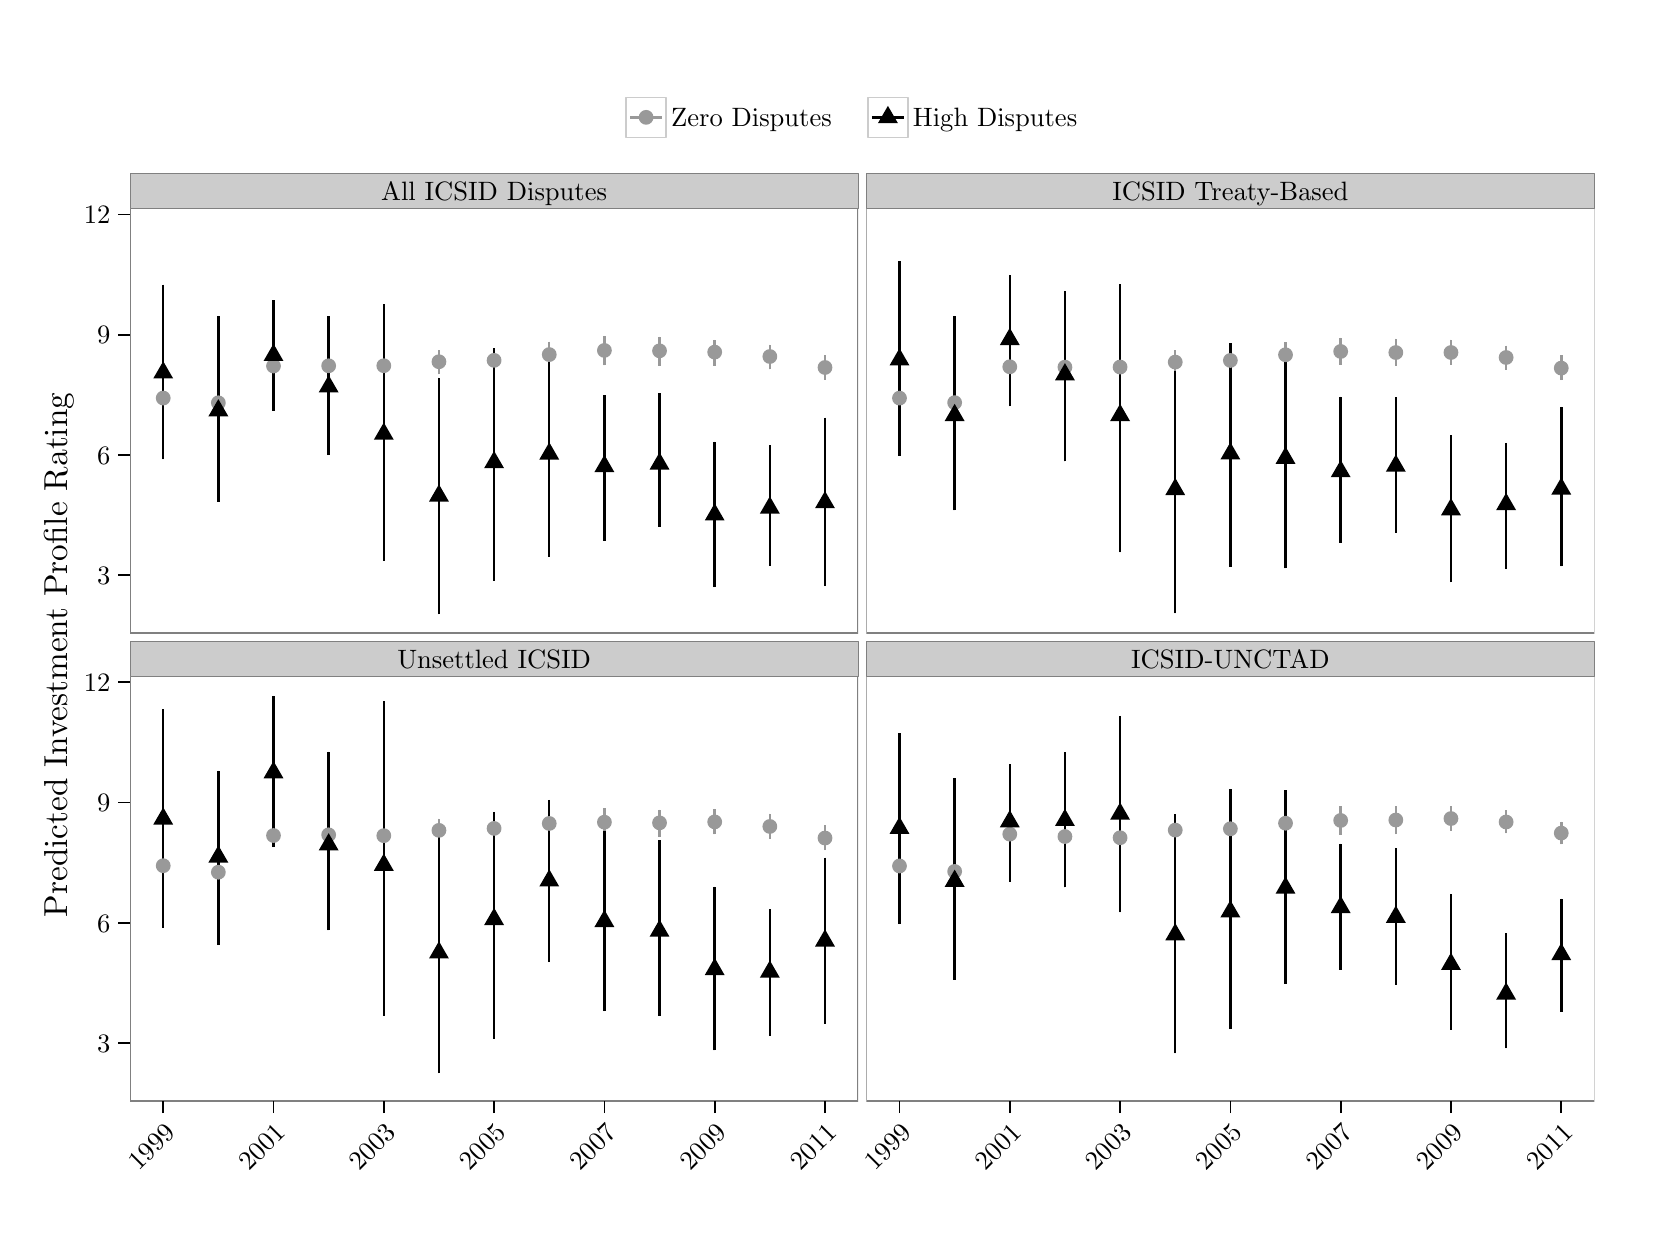
\begin{tikzpicture}[x=1pt,y=1pt]
\definecolor[named]{fillColor}{rgb}{1.00,1.00,1.00}
\path[use as bounding box,fill=fillColor,fill opacity=0.00] (0,0) rectangle (578.16,433.62);
\begin{scope}
\path[clip] (  0.00,  0.00) rectangle (578.16,433.62);
\definecolor[named]{drawColor}{rgb}{1.00,1.00,1.00}
\definecolor[named]{fillColor}{rgb}{1.00,1.00,1.00}

\path[draw=drawColor,line width= 0.6pt,line join=round,line cap=round,fill=fillColor] (  0.00,  0.00) rectangle (578.16,433.62);
\end{scope}
\begin{scope}
\path[clip] ( 37.02,214.77) rectangle (300.06,368.22);
\definecolor[named]{fillColor}{rgb}{1.00,1.00,1.00}

\path[fill=fillColor] ( 37.02,214.77) rectangle (300.06,368.22);
\definecolor[named]{drawColor}{rgb}{0.60,0.60,0.60}
\definecolor[named]{fillColor}{rgb}{0.60,0.60,0.60}

\path[draw=drawColor,line width= 0.9pt,line join=round,fill=fillColor] ( 48.98,293.67) -- ( 48.98,305.59);

\path[draw=drawColor,line width= 0.9pt,line join=round,fill=fillColor] ( 68.90,291.93) -- ( 68.90,304.29);

\path[draw=drawColor,line width= 0.9pt,line join=round,fill=fillColor] ( 88.83,307.70) -- ( 88.83,315.07);

\path[draw=drawColor,line width= 0.9pt,line join=round,fill=fillColor] (108.76,305.93) -- (108.76,317.28);

\path[draw=drawColor,line width= 0.9pt,line join=round,fill=fillColor] (128.69,306.46) -- (128.69,316.72);

\path[draw=drawColor,line width= 0.9pt,line join=round,fill=fillColor] (148.61,308.45) -- (148.61,317.07);

\path[draw=drawColor,line width= 0.9pt,line join=round,fill=fillColor] (168.54,309.24) -- (168.54,317.81);

\path[draw=drawColor,line width= 0.9pt,line join=round,fill=fillColor] (188.47,310.64) -- (188.47,320.16);

\path[draw=drawColor,line width= 0.9pt,line join=round,fill=fillColor] (208.40,311.61) -- (208.40,322.25);

\path[draw=drawColor,line width= 0.9pt,line join=round,fill=fillColor] (228.32,311.45) -- (228.32,321.98);

\path[draw=drawColor,line width= 0.9pt,line join=round,fill=fillColor] (248.25,311.52) -- (248.25,320.82);

\path[draw=drawColor,line width= 0.9pt,line join=round,fill=fillColor] (268.18,310.10) -- (268.18,319.07);

\path[draw=drawColor,line width= 0.9pt,line join=round,fill=fillColor] (288.11,306.38) -- (288.11,315.18);
\definecolor[named]{drawColor}{rgb}{0.00,0.00,0.00}
\definecolor[named]{fillColor}{rgb}{0.00,0.00,0.00}

\path[draw=drawColor,line width= 0.9pt,line join=round,fill=fillColor] ( 48.98,277.65) -- ( 48.98,340.81);

\path[draw=drawColor,line width= 0.9pt,line join=round,fill=fillColor] ( 68.90,262.34) -- ( 68.90,329.49);

\path[draw=drawColor,line width= 0.9pt,line join=round,fill=fillColor] ( 88.83,295.23) -- ( 88.83,335.12);

\path[draw=drawColor,line width= 0.9pt,line join=round,fill=fillColor] (108.76,279.19) -- (108.76,329.36);

\path[draw=drawColor,line width= 0.9pt,line join=round,fill=fillColor] (128.69,240.98) -- (128.69,333.61);

\path[draw=drawColor,line width= 0.9pt,line join=round,fill=fillColor] (148.61,221.74) -- (148.61,307.17);

\path[draw=drawColor,line width= 0.9pt,line join=round,fill=fillColor] (168.54,233.78) -- (168.54,317.86);

\path[draw=drawColor,line width= 0.9pt,line join=round,fill=fillColor] (188.47,242.46) -- (188.47,316.24);

\path[draw=drawColor,line width= 0.9pt,line join=round,fill=fillColor] (208.40,248.30) -- (208.40,300.81);

\path[draw=drawColor,line width= 0.9pt,line join=round,fill=fillColor] (228.32,253.28) -- (228.32,301.49);

\path[draw=drawColor,line width= 0.9pt,line join=round,fill=fillColor] (248.25,231.43) -- (248.25,284.04);

\path[draw=drawColor,line width= 0.9pt,line join=round,fill=fillColor] (268.18,239.20) -- (268.18,282.77);

\path[draw=drawColor,line width= 0.9pt,line join=round,fill=fillColor] (288.11,231.84) -- (288.11,292.68);
\definecolor[named]{fillColor}{rgb}{0.60,0.60,0.60}

\path[fill=fillColor] ( 48.98,299.78) circle (  2.67);
\definecolor[named]{fillColor}{rgb}{0.00,0.00,0.00}

\path[fill=fillColor] ( 48.98,313.08) --
	( 52.57,306.86) --
	( 45.38,306.86) --
	cycle;
\definecolor[named]{fillColor}{rgb}{0.60,0.60,0.60}

\path[fill=fillColor] ( 68.90,298.06) circle (  2.67);
\definecolor[named]{fillColor}{rgb}{0.00,0.00,0.00}

\path[fill=fillColor] ( 68.90,299.40) --
	( 72.50,293.18) --
	( 65.31,293.18) --
	cycle;
\definecolor[named]{fillColor}{rgb}{0.60,0.60,0.60}

\path[fill=fillColor] ( 88.83,311.37) circle (  2.67);
\definecolor[named]{fillColor}{rgb}{0.00,0.00,0.00}

\path[fill=fillColor] ( 88.83,319.41) --
	( 92.42,313.18) --
	( 85.24,313.18) --
	cycle;
\definecolor[named]{fillColor}{rgb}{0.60,0.60,0.60}

\path[fill=fillColor] (108.76,311.43) circle (  2.67);
\definecolor[named]{fillColor}{rgb}{0.00,0.00,0.00}

\path[fill=fillColor] (108.76,308.05) --
	(112.35,301.83) --
	(105.17,301.83) --
	cycle;
\definecolor[named]{fillColor}{rgb}{0.60,0.60,0.60}

\path[fill=fillColor] (128.69,311.46) circle (  2.67);
\definecolor[named]{fillColor}{rgb}{0.00,0.00,0.00}

\path[fill=fillColor] (128.69,290.94) --
	(132.28,284.72) --
	(125.09,284.72) --
	cycle;
\definecolor[named]{fillColor}{rgb}{0.60,0.60,0.60}

\path[fill=fillColor] (148.61,312.90) circle (  2.67);
\definecolor[named]{fillColor}{rgb}{0.00,0.00,0.00}

\path[fill=fillColor] (148.61,268.61) --
	(152.21,262.38) --
	(145.02,262.38) --
	cycle;
\definecolor[named]{fillColor}{rgb}{0.60,0.60,0.60}

\path[fill=fillColor] (168.54,313.40) circle (  2.67);
\definecolor[named]{fillColor}{rgb}{0.00,0.00,0.00}

\path[fill=fillColor] (168.54,280.68) --
	(172.13,274.46) --
	(164.95,274.46) --
	cycle;
\definecolor[named]{fillColor}{rgb}{0.60,0.60,0.60}

\path[fill=fillColor] (188.47,315.49) circle (  2.67);
\definecolor[named]{fillColor}{rgb}{0.00,0.00,0.00}

\path[fill=fillColor] (188.47,283.79) --
	(192.06,277.57) --
	(184.88,277.57) --
	cycle;
\definecolor[named]{fillColor}{rgb}{0.60,0.60,0.60}

\path[fill=fillColor] (208.40,316.99) circle (  2.67);
\definecolor[named]{fillColor}{rgb}{0.00,0.00,0.00}

\path[fill=fillColor] (208.40,279.25) --
	(211.99,273.03) --
	(204.80,273.03) --
	cycle;
\definecolor[named]{fillColor}{rgb}{0.60,0.60,0.60}

\path[fill=fillColor] (228.32,316.84) circle (  2.67);
\definecolor[named]{fillColor}{rgb}{0.00,0.00,0.00}

\path[fill=fillColor] (228.32,280.17) --
	(231.92,273.95) --
	(224.73,273.95) --
	cycle;
\definecolor[named]{fillColor}{rgb}{0.60,0.60,0.60}

\path[fill=fillColor] (248.25,316.38) circle (  2.67);
\definecolor[named]{fillColor}{rgb}{0.00,0.00,0.00}

\path[fill=fillColor] (248.25,261.76) --
	(251.84,255.54) --
	(244.66,255.54) --
	cycle;
\definecolor[named]{fillColor}{rgb}{0.60,0.60,0.60}

\path[fill=fillColor] (268.18,314.79) circle (  2.67);
\definecolor[named]{fillColor}{rgb}{0.00,0.00,0.00}

\path[fill=fillColor] (268.18,264.27) --
	(271.77,258.04) --
	(264.59,258.04) --
	cycle;
\definecolor[named]{fillColor}{rgb}{0.60,0.60,0.60}

\path[fill=fillColor] (288.11,310.83) circle (  2.67);
\definecolor[named]{fillColor}{rgb}{0.00,0.00,0.00}

\path[fill=fillColor] (288.11,266.20) --
	(291.70,259.97) --
	(284.51,259.97) --
	cycle;
\definecolor[named]{drawColor}{rgb}{0.50,0.50,0.50}

\path[draw=drawColor,line width= 0.6pt,line join=round,line cap=round] ( 37.02,214.77) rectangle (300.06,368.22);
\end{scope}
\begin{scope}
\path[clip] (303.07,214.77) rectangle (566.12,368.22);
\definecolor[named]{fillColor}{rgb}{1.00,1.00,1.00}

\path[fill=fillColor] (303.07,214.77) rectangle (566.12,368.22);
\definecolor[named]{drawColor}{rgb}{0.60,0.60,0.60}
\definecolor[named]{fillColor}{rgb}{0.60,0.60,0.60}

\path[draw=drawColor,line width= 0.9pt,line join=round,fill=fillColor] (315.03,293.78) -- (315.03,305.84);

\path[draw=drawColor,line width= 0.9pt,line join=round,fill=fillColor] (334.96,291.95) -- (334.96,304.13);

\path[draw=drawColor,line width= 0.9pt,line join=round,fill=fillColor] (354.88,307.16) -- (354.88,314.84);

\path[draw=drawColor,line width= 0.9pt,line join=round,fill=fillColor] (374.81,305.98) -- (374.81,316.10);

\path[draw=drawColor,line width= 0.9pt,line join=round,fill=fillColor] (394.74,305.73) -- (394.74,316.18);

\path[draw=drawColor,line width= 0.9pt,line join=round,fill=fillColor] (414.67,308.47) -- (414.67,316.99);

\path[draw=drawColor,line width= 0.9pt,line join=round,fill=fillColor] (434.59,309.08) -- (434.59,317.58);

\path[draw=drawColor,line width= 0.9pt,line join=round,fill=fillColor] (454.52,310.77) -- (454.52,319.96);

\path[draw=drawColor,line width= 0.9pt,line join=round,fill=fillColor] (474.45,311.76) -- (474.45,321.65);

\path[draw=drawColor,line width= 0.9pt,line join=round,fill=fillColor] (494.38,311.49) -- (494.38,321.25);

\path[draw=drawColor,line width= 0.9pt,line join=round,fill=fillColor] (514.30,311.80) -- (514.30,320.87);

\path[draw=drawColor,line width= 0.9pt,line join=round,fill=fillColor] (534.23,310.00) -- (534.23,318.75);

\path[draw=drawColor,line width= 0.9pt,line join=round,fill=fillColor] (554.16,306.27) -- (554.16,315.18);
\definecolor[named]{drawColor}{rgb}{0.00,0.00,0.00}
\definecolor[named]{fillColor}{rgb}{0.00,0.00,0.00}

\path[draw=drawColor,line width= 0.9pt,line join=round,fill=fillColor] (315.03,278.99) -- (315.03,349.30);

\path[draw=drawColor,line width= 0.9pt,line join=round,fill=fillColor] (334.96,259.18) -- (334.96,329.45);

\path[draw=drawColor,line width= 0.9pt,line join=round,fill=fillColor] (354.88,296.83) -- (354.88,344.32);

\path[draw=drawColor,line width= 0.9pt,line join=round,fill=fillColor] (374.81,276.90) -- (374.81,338.49);

\path[draw=drawColor,line width= 0.9pt,line join=round,fill=fillColor] (394.74,243.99) -- (394.74,340.82);

\path[draw=drawColor,line width= 0.9pt,line join=round,fill=fillColor] (414.67,221.97) -- (414.67,309.69);

\path[draw=drawColor,line width= 0.9pt,line join=round,fill=fillColor] (434.59,238.83) -- (434.59,319.61);

\path[draw=drawColor,line width= 0.9pt,line join=round,fill=fillColor] (454.52,238.22) -- (454.52,316.91);

\path[draw=drawColor,line width= 0.9pt,line join=round,fill=fillColor] (474.45,247.41) -- (474.45,300.28);

\path[draw=drawColor,line width= 0.9pt,line join=round,fill=fillColor] (494.38,251.06) -- (494.38,300.07);

\path[draw=drawColor,line width= 0.9pt,line join=round,fill=fillColor] (514.30,233.31) -- (514.30,286.29);

\path[draw=drawColor,line width= 0.9pt,line join=round,fill=fillColor] (534.23,238.00) -- (534.23,283.55);

\path[draw=drawColor,line width= 0.9pt,line join=round,fill=fillColor] (554.16,238.96) -- (554.16,296.55);
\definecolor[named]{fillColor}{rgb}{0.60,0.60,0.60}

\path[fill=fillColor] (315.03,299.76) circle (  2.67);
\definecolor[named]{fillColor}{rgb}{0.00,0.00,0.00}

\path[fill=fillColor] (315.03,317.80) --
	(318.62,311.58) --
	(311.44,311.58) --
	cycle;
\definecolor[named]{fillColor}{rgb}{0.60,0.60,0.60}

\path[fill=fillColor] (334.96,298.12) circle (  2.67);
\definecolor[named]{fillColor}{rgb}{0.00,0.00,0.00}

\path[fill=fillColor] (334.96,297.70) --
	(338.55,291.48) --
	(331.36,291.48) --
	cycle;
\definecolor[named]{fillColor}{rgb}{0.60,0.60,0.60}

\path[fill=fillColor] (354.88,311.08) circle (  2.67);
\definecolor[named]{fillColor}{rgb}{0.00,0.00,0.00}

\path[fill=fillColor] (354.88,325.15) --
	(358.48,318.92) --
	(351.29,318.92) --
	cycle;
\definecolor[named]{fillColor}{rgb}{0.60,0.60,0.60}

\path[fill=fillColor] (374.81,310.94) circle (  2.67);
\definecolor[named]{fillColor}{rgb}{0.00,0.00,0.00}

\path[fill=fillColor] (374.81,312.41) --
	(378.40,306.19) --
	(371.22,306.19) --
	cycle;
\definecolor[named]{fillColor}{rgb}{0.60,0.60,0.60}

\path[fill=fillColor] (394.74,310.98) circle (  2.67);
\definecolor[named]{fillColor}{rgb}{0.00,0.00,0.00}

\path[fill=fillColor] (394.74,297.69) --
	(398.33,291.47) --
	(391.15,291.47) --
	cycle;
\definecolor[named]{fillColor}{rgb}{0.60,0.60,0.60}

\path[fill=fillColor] (414.67,312.77) circle (  2.67);
\definecolor[named]{fillColor}{rgb}{0.00,0.00,0.00}

\path[fill=fillColor] (414.67,270.93) --
	(418.26,264.71) --
	(411.07,264.71) --
	cycle;
\definecolor[named]{fillColor}{rgb}{0.60,0.60,0.60}

\path[fill=fillColor] (434.59,313.37) circle (  2.67);
\definecolor[named]{fillColor}{rgb}{0.00,0.00,0.00}

\path[fill=fillColor] (434.59,283.82) --
	(438.19,277.59) --
	(431.00,277.59) --
	cycle;
\definecolor[named]{fillColor}{rgb}{0.60,0.60,0.60}

\path[fill=fillColor] (454.52,315.42) circle (  2.67);
\definecolor[named]{fillColor}{rgb}{0.00,0.00,0.00}

\path[fill=fillColor] (454.52,282.24) --
	(458.11,276.02) --
	(450.93,276.02) --
	cycle;
\definecolor[named]{fillColor}{rgb}{0.60,0.60,0.60}

\path[fill=fillColor] (474.45,316.62) circle (  2.67);
\definecolor[named]{fillColor}{rgb}{0.00,0.00,0.00}

\path[fill=fillColor] (474.45,277.40) --
	(478.04,271.18) --
	(470.86,271.18) --
	cycle;
\definecolor[named]{fillColor}{rgb}{0.60,0.60,0.60}

\path[fill=fillColor] (494.38,316.22) circle (  2.67);
\definecolor[named]{fillColor}{rgb}{0.00,0.00,0.00}

\path[fill=fillColor] (494.38,279.40) --
	(497.97,273.18) --
	(490.78,273.18) --
	cycle;
\definecolor[named]{fillColor}{rgb}{0.60,0.60,0.60}

\path[fill=fillColor] (514.30,316.24) circle (  2.67);
\definecolor[named]{fillColor}{rgb}{0.00,0.00,0.00}

\path[fill=fillColor] (514.30,263.64) --
	(517.90,257.42) --
	(510.71,257.42) --
	cycle;
\definecolor[named]{fillColor}{rgb}{0.60,0.60,0.60}

\path[fill=fillColor] (534.23,314.44) circle (  2.67);
\definecolor[named]{fillColor}{rgb}{0.00,0.00,0.00}

\path[fill=fillColor] (534.23,265.53) --
	(537.82,259.31) --
	(530.64,259.31) --
	cycle;
\definecolor[named]{fillColor}{rgb}{0.60,0.60,0.60}

\path[fill=fillColor] (554.16,310.60) circle (  2.67);
\definecolor[named]{fillColor}{rgb}{0.00,0.00,0.00}

\path[fill=fillColor] (554.16,271.14) --
	(557.75,264.92) --
	(550.57,264.92) --
	cycle;
\definecolor[named]{drawColor}{rgb}{0.50,0.50,0.50}

\path[draw=drawColor,line width= 0.6pt,line join=round,line cap=round] (303.07,214.77) rectangle (566.12,368.22);
\end{scope}
\begin{scope}
\path[clip] ( 37.02, 45.67) rectangle (300.06,199.12);
\definecolor[named]{fillColor}{rgb}{1.00,1.00,1.00}

\path[fill=fillColor] ( 37.02, 45.67) rectangle (300.06,199.12);
\definecolor[named]{drawColor}{rgb}{0.60,0.60,0.60}
\definecolor[named]{fillColor}{rgb}{0.60,0.60,0.60}

\path[draw=drawColor,line width= 0.9pt,line join=round,fill=fillColor] ( 48.98,125.38) -- ( 48.98,136.64);

\path[draw=drawColor,line width= 0.9pt,line join=round,fill=fillColor] ( 68.90,122.62) -- ( 68.90,134.68);

\path[draw=drawColor,line width= 0.9pt,line join=round,fill=fillColor] ( 88.83,137.99) -- ( 88.83,145.38);

\path[draw=drawColor,line width= 0.9pt,line join=round,fill=fillColor] (108.76,136.92) -- (108.76,146.80);

\path[draw=drawColor,line width= 0.9pt,line join=round,fill=fillColor] (128.69,136.43) -- (128.69,146.97);

\path[draw=drawColor,line width= 0.9pt,line join=round,fill=fillColor] (148.61,139.21) -- (148.61,147.84);

\path[draw=drawColor,line width= 0.9pt,line join=round,fill=fillColor] (168.54,139.98) -- (168.54,148.92);

\path[draw=drawColor,line width= 0.9pt,line join=round,fill=fillColor] (188.47,141.35) -- (188.47,150.56);

\path[draw=drawColor,line width= 0.9pt,line join=round,fill=fillColor] (208.40,141.52) -- (208.40,151.53);

\path[draw=drawColor,line width= 0.9pt,line join=round,fill=fillColor] (228.32,141.08) -- (228.32,151.10);

\path[draw=drawColor,line width= 0.9pt,line join=round,fill=fillColor] (248.25,142.10) -- (248.25,151.31);

\path[draw=drawColor,line width= 0.9pt,line join=round,fill=fillColor] (268.18,140.56) -- (268.18,149.61);

\path[draw=drawColor,line width= 0.9pt,line join=round,fill=fillColor] (288.11,136.44) -- (288.11,145.36);
\definecolor[named]{drawColor}{rgb}{0.00,0.00,0.00}
\definecolor[named]{fillColor}{rgb}{0.00,0.00,0.00}

\path[draw=drawColor,line width= 0.9pt,line join=round,fill=fillColor] ( 48.98,108.37) -- ( 48.98,187.25);

\path[draw=drawColor,line width= 0.9pt,line join=round,fill=fillColor] ( 68.90,102.13) -- ( 68.90,165.18);

\path[draw=drawColor,line width= 0.9pt,line join=round,fill=fillColor] ( 88.83,137.47) -- ( 88.83,192.15);

\path[draw=drawColor,line width= 0.9pt,line join=round,fill=fillColor] (108.76,107.39) -- (108.76,171.99);

\path[draw=drawColor,line width= 0.9pt,line join=round,fill=fillColor] (128.69, 76.50) -- (128.69,190.14);

\path[draw=drawColor,line width= 0.9pt,line join=round,fill=fillColor] (148.61, 55.81) -- (148.61,142.68);

\path[draw=drawColor,line width= 0.9pt,line join=round,fill=fillColor] (168.54, 68.20) -- (168.54,150.27);

\path[draw=drawColor,line width= 0.9pt,line join=round,fill=fillColor] (188.47, 95.95) -- (188.47,154.62);

\path[draw=drawColor,line width= 0.9pt,line join=round,fill=fillColor] (208.40, 78.21) -- (208.40,143.42);

\path[draw=drawColor,line width= 0.9pt,line join=round,fill=fillColor] (228.32, 76.53) -- (228.32,140.01);

\path[draw=drawColor,line width= 0.9pt,line join=round,fill=fillColor] (248.25, 64.08) -- (248.25,123.27);

\path[draw=drawColor,line width= 0.9pt,line join=round,fill=fillColor] (268.18, 69.38) -- (268.18,115.03);

\path[draw=drawColor,line width= 0.9pt,line join=round,fill=fillColor] (288.11, 73.63) -- (288.11,133.71);
\definecolor[named]{fillColor}{rgb}{0.60,0.60,0.60}

\path[fill=fillColor] ( 48.98,130.79) circle (  2.67);
\definecolor[named]{fillColor}{rgb}{0.00,0.00,0.00}

\path[fill=fillColor] ( 48.98,151.88) --
	( 52.57,145.66) --
	( 45.38,145.66) --
	cycle;
\definecolor[named]{fillColor}{rgb}{0.60,0.60,0.60}

\path[fill=fillColor] ( 68.90,128.45) circle (  2.67);
\definecolor[named]{fillColor}{rgb}{0.00,0.00,0.00}

\path[fill=fillColor] ( 68.90,138.16) --
	( 72.50,131.93) --
	( 65.31,131.93) --
	cycle;
\definecolor[named]{fillColor}{rgb}{0.60,0.60,0.60}

\path[fill=fillColor] ( 88.83,141.70) circle (  2.67);
\definecolor[named]{fillColor}{rgb}{0.00,0.00,0.00}

\path[fill=fillColor] ( 88.83,168.61) --
	( 92.42,162.39) --
	( 85.24,162.39) --
	cycle;
\definecolor[named]{fillColor}{rgb}{0.60,0.60,0.60}

\path[fill=fillColor] (108.76,141.95) circle (  2.67);
\definecolor[named]{fillColor}{rgb}{0.00,0.00,0.00}

\path[fill=fillColor] (108.76,142.56) --
	(112.35,136.34) --
	(105.17,136.34) --
	cycle;
\definecolor[named]{fillColor}{rgb}{0.60,0.60,0.60}

\path[fill=fillColor] (128.69,141.65) circle (  2.67);
\definecolor[named]{fillColor}{rgb}{0.00,0.00,0.00}

\path[fill=fillColor] (128.69,135.19) --
	(132.28,128.97) --
	(125.09,128.97) --
	cycle;
\definecolor[named]{fillColor}{rgb}{0.60,0.60,0.60}

\path[fill=fillColor] (148.61,143.57) circle (  2.67);
\definecolor[named]{fillColor}{rgb}{0.00,0.00,0.00}

\path[fill=fillColor] (148.61,103.50) --
	(152.21, 97.28) --
	(145.02, 97.28) --
	cycle;
\definecolor[named]{fillColor}{rgb}{0.60,0.60,0.60}

\path[fill=fillColor] (168.54,144.27) circle (  2.67);
\definecolor[named]{fillColor}{rgb}{0.00,0.00,0.00}

\path[fill=fillColor] (168.54,115.58) --
	(172.13,109.36) --
	(164.95,109.36) --
	cycle;
\definecolor[named]{fillColor}{rgb}{0.60,0.60,0.60}

\path[fill=fillColor] (188.47,146.06) circle (  2.67);
\definecolor[named]{fillColor}{rgb}{0.00,0.00,0.00}

\path[fill=fillColor] (188.47,129.51) --
	(192.06,123.29) --
	(184.88,123.29) --
	cycle;
\definecolor[named]{fillColor}{rgb}{0.60,0.60,0.60}

\path[fill=fillColor] (208.40,146.52) circle (  2.67);
\definecolor[named]{fillColor}{rgb}{0.00,0.00,0.00}

\path[fill=fillColor] (208.40,114.87) --
	(211.99,108.64) --
	(204.80,108.64) --
	cycle;
\definecolor[named]{fillColor}{rgb}{0.60,0.60,0.60}

\path[fill=fillColor] (228.32,146.28) circle (  2.67);
\definecolor[named]{fillColor}{rgb}{0.00,0.00,0.00}

\path[fill=fillColor] (228.32,111.36) --
	(231.92,105.14) --
	(224.73,105.14) --
	cycle;
\definecolor[named]{fillColor}{rgb}{0.60,0.60,0.60}

\path[fill=fillColor] (248.25,146.63) circle (  2.67);
\definecolor[named]{fillColor}{rgb}{0.00,0.00,0.00}

\path[fill=fillColor] (248.25, 97.50) --
	(251.84, 91.27) --
	(244.66, 91.27) --
	cycle;
\definecolor[named]{fillColor}{rgb}{0.60,0.60,0.60}

\path[fill=fillColor] (268.18,144.98) circle (  2.67);
\definecolor[named]{fillColor}{rgb}{0.00,0.00,0.00}

\path[fill=fillColor] (268.18, 96.58) --
	(271.77, 90.36) --
	(264.59, 90.36) --
	cycle;
\definecolor[named]{fillColor}{rgb}{0.60,0.60,0.60}

\path[fill=fillColor] (288.11,140.79) circle (  2.67);
\definecolor[named]{fillColor}{rgb}{0.00,0.00,0.00}

\path[fill=fillColor] (288.11,107.82) --
	(291.70,101.60) --
	(284.51,101.60) --
	cycle;
\definecolor[named]{drawColor}{rgb}{0.50,0.50,0.50}

\path[draw=drawColor,line width= 0.6pt,line join=round,line cap=round] ( 37.02, 45.67) rectangle (300.06,199.12);
\end{scope}
\begin{scope}
\path[clip] (303.07, 45.67) rectangle (566.12,199.12);
\definecolor[named]{fillColor}{rgb}{1.00,1.00,1.00}

\path[fill=fillColor] (303.07, 45.67) rectangle (566.12,199.12);
\definecolor[named]{drawColor}{rgb}{0.60,0.60,0.60}
\definecolor[named]{fillColor}{rgb}{0.60,0.60,0.60}

\path[draw=drawColor,line width= 0.9pt,line join=round,fill=fillColor] (315.03,124.77) -- (315.03,136.40);

\path[draw=drawColor,line width= 0.9pt,line join=round,fill=fillColor] (334.96,122.55) -- (334.96,134.49);

\path[draw=drawColor,line width= 0.9pt,line join=round,fill=fillColor] (354.88,138.58) -- (354.88,146.09);

\path[draw=drawColor,line width= 0.9pt,line join=round,fill=fillColor] (374.81,135.46) -- (374.81,146.59);

\path[draw=drawColor,line width= 0.9pt,line join=round,fill=fillColor] (394.74,135.88) -- (394.74,145.95);

\path[draw=drawColor,line width= 0.9pt,line join=round,fill=fillColor] (414.67,139.39) -- (414.67,147.97);

\path[draw=drawColor,line width= 0.9pt,line join=round,fill=fillColor] (434.59,139.78) -- (434.59,148.45);

\path[draw=drawColor,line width= 0.9pt,line join=round,fill=fillColor] (454.52,141.53) -- (454.52,150.88);

\path[draw=drawColor,line width= 0.9pt,line join=round,fill=fillColor] (474.45,141.91) -- (474.45,152.29);

\path[draw=drawColor,line width= 0.9pt,line join=round,fill=fillColor] (494.38,142.20) -- (494.38,152.36);

\path[draw=drawColor,line width= 0.9pt,line join=round,fill=fillColor] (514.30,143.35) -- (514.30,152.28);

\path[draw=drawColor,line width= 0.9pt,line join=round,fill=fillColor] (534.23,142.45) -- (534.23,150.85);

\path[draw=drawColor,line width= 0.9pt,line join=round,fill=fillColor] (554.16,138.48) -- (554.16,146.68);
\definecolor[named]{drawColor}{rgb}{0.00,0.00,0.00}
\definecolor[named]{fillColor}{rgb}{0.00,0.00,0.00}

\path[draw=drawColor,line width= 0.9pt,line join=round,fill=fillColor] (315.03,109.70) -- (315.03,178.73);

\path[draw=drawColor,line width= 0.9pt,line join=round,fill=fillColor] (334.96, 89.60) -- (334.96,162.56);

\path[draw=drawColor,line width= 0.9pt,line join=round,fill=fillColor] (354.88,124.91) -- (354.88,167.47);

\path[draw=drawColor,line width= 0.9pt,line join=round,fill=fillColor] (374.81,122.92) -- (374.81,171.79);

\path[draw=drawColor,line width= 0.9pt,line join=round,fill=fillColor] (394.74,113.96) -- (394.74,184.97);

\path[draw=drawColor,line width= 0.9pt,line join=round,fill=fillColor] (414.67, 62.98) -- (414.67,149.42);

\path[draw=drawColor,line width= 0.9pt,line join=round,fill=fillColor] (434.59, 71.72) -- (434.59,158.52);

\path[draw=drawColor,line width= 0.9pt,line join=round,fill=fillColor] (454.52, 88.23) -- (454.52,158.15);

\path[draw=drawColor,line width= 0.9pt,line join=round,fill=fillColor] (474.45, 93.25) -- (474.45,138.81);

\path[draw=drawColor,line width= 0.9pt,line join=round,fill=fillColor] (494.38, 87.78) -- (494.38,137.21);

\path[draw=drawColor,line width= 0.9pt,line join=round,fill=fillColor] (514.30, 71.48) -- (514.30,120.63);

\path[draw=drawColor,line width= 0.9pt,line join=round,fill=fillColor] (534.23, 64.78) -- (534.23,106.32);

\path[draw=drawColor,line width= 0.9pt,line join=round,fill=fillColor] (554.16, 77.99) -- (554.16,118.94);
\definecolor[named]{fillColor}{rgb}{0.60,0.60,0.60}

\path[fill=fillColor] (315.03,130.70) circle (  2.67);
\definecolor[named]{fillColor}{rgb}{0.00,0.00,0.00}

\path[fill=fillColor] (315.03,148.52) --
	(318.62,142.30) --
	(311.44,142.30) --
	cycle;
\definecolor[named]{fillColor}{rgb}{0.60,0.60,0.60}

\path[fill=fillColor] (334.96,128.73) circle (  2.67);
\definecolor[named]{fillColor}{rgb}{0.00,0.00,0.00}

\path[fill=fillColor] (334.96,129.39) --
	(338.55,123.16) --
	(331.36,123.16) --
	cycle;
\definecolor[named]{fillColor}{rgb}{0.60,0.60,0.60}

\path[fill=fillColor] (354.88,142.20) circle (  2.67);
\definecolor[named]{fillColor}{rgb}{0.00,0.00,0.00}

\path[fill=fillColor] (354.88,150.89) --
	(358.48,144.67) --
	(351.29,144.67) --
	cycle;
\definecolor[named]{fillColor}{rgb}{0.60,0.60,0.60}

\path[fill=fillColor] (374.81,141.34) circle (  2.67);
\definecolor[named]{fillColor}{rgb}{0.00,0.00,0.00}

\path[fill=fillColor] (374.81,151.38) --
	(378.40,145.16) --
	(371.22,145.16) --
	cycle;
\definecolor[named]{fillColor}{rgb}{0.60,0.60,0.60}

\path[fill=fillColor] (394.74,140.90) circle (  2.67);
\definecolor[named]{fillColor}{rgb}{0.00,0.00,0.00}

\path[fill=fillColor] (394.74,153.66) --
	(398.33,147.43) --
	(391.15,147.43) --
	cycle;
\definecolor[named]{fillColor}{rgb}{0.60,0.60,0.60}

\path[fill=fillColor] (414.67,143.66) circle (  2.67);
\definecolor[named]{fillColor}{rgb}{0.00,0.00,0.00}

\path[fill=fillColor] (414.67,110.05) --
	(418.26,103.83) --
	(411.07,103.83) --
	cycle;
\definecolor[named]{fillColor}{rgb}{0.60,0.60,0.60}

\path[fill=fillColor] (434.59,144.13) circle (  2.67);
\definecolor[named]{fillColor}{rgb}{0.00,0.00,0.00}

\path[fill=fillColor] (434.59,118.36) --
	(438.19,112.14) --
	(431.00,112.14) --
	cycle;
\definecolor[named]{fillColor}{rgb}{0.60,0.60,0.60}

\path[fill=fillColor] (454.52,146.15) circle (  2.67);
\definecolor[named]{fillColor}{rgb}{0.00,0.00,0.00}

\path[fill=fillColor] (454.52,126.92) --
	(458.11,120.70) --
	(450.93,120.70) --
	cycle;
\definecolor[named]{fillColor}{rgb}{0.60,0.60,0.60}

\path[fill=fillColor] (474.45,147.15) circle (  2.67);
\definecolor[named]{fillColor}{rgb}{0.00,0.00,0.00}

\path[fill=fillColor] (474.45,119.91) --
	(478.04,113.69) --
	(470.86,113.69) --
	cycle;
\definecolor[named]{fillColor}{rgb}{0.60,0.60,0.60}

\path[fill=fillColor] (494.38,147.30) circle (  2.67);
\definecolor[named]{fillColor}{rgb}{0.00,0.00,0.00}

\path[fill=fillColor] (494.38,116.40) --
	(497.97,110.17) --
	(490.78,110.17) --
	cycle;
\definecolor[named]{fillColor}{rgb}{0.60,0.60,0.60}

\path[fill=fillColor] (514.30,147.83) circle (  2.67);
\definecolor[named]{fillColor}{rgb}{0.00,0.00,0.00}

\path[fill=fillColor] (514.30, 99.36) --
	(517.90, 93.13) --
	(510.71, 93.13) --
	cycle;
\definecolor[named]{fillColor}{rgb}{0.60,0.60,0.60}

\path[fill=fillColor] (534.23,146.59) circle (  2.67);
\definecolor[named]{fillColor}{rgb}{0.00,0.00,0.00}

\path[fill=fillColor] (534.23, 88.64) --
	(537.82, 82.42) --
	(530.64, 82.42) --
	cycle;
\definecolor[named]{fillColor}{rgb}{0.60,0.60,0.60}

\path[fill=fillColor] (554.16,142.58) circle (  2.67);
\definecolor[named]{fillColor}{rgb}{0.00,0.00,0.00}

\path[fill=fillColor] (554.16,102.90) --
	(557.75, 96.68) --
	(550.57, 96.68) --
	cycle;
\definecolor[named]{drawColor}{rgb}{0.50,0.50,0.50}

\path[draw=drawColor,line width= 0.6pt,line join=round,line cap=round] (303.07, 45.67) rectangle (566.12,199.12);
\end{scope}
\begin{scope}
\path[clip] (  0.00,  0.00) rectangle (578.16,433.62);
\definecolor[named]{drawColor}{rgb}{0.50,0.50,0.50}
\definecolor[named]{fillColor}{rgb}{0.80,0.80,0.80}

\path[draw=drawColor,line width= 0.2pt,line join=round,line cap=round,fill=fillColor] ( 37.02,368.22) rectangle (300.06,380.85);
\definecolor[named]{drawColor}{rgb}{0.00,0.00,0.00}

\node[text=drawColor,anchor=base,inner sep=0pt, outer sep=0pt, scale=  0.96] at (168.54,371.23) {All ICSID Disputes};
\end{scope}
\begin{scope}
\path[clip] (  0.00,  0.00) rectangle (578.16,433.62);
\definecolor[named]{drawColor}{rgb}{0.50,0.50,0.50}
\definecolor[named]{fillColor}{rgb}{0.80,0.80,0.80}

\path[draw=drawColor,line width= 0.2pt,line join=round,line cap=round,fill=fillColor] (303.07,368.22) rectangle (566.12,380.85);
\definecolor[named]{drawColor}{rgb}{0.00,0.00,0.00}

\node[text=drawColor,anchor=base,inner sep=0pt, outer sep=0pt, scale=  0.96] at (434.59,371.23) {ICSID Treaty-Based};
\end{scope}
\begin{scope}
\path[clip] (  0.00,  0.00) rectangle (578.16,433.62);
\definecolor[named]{drawColor}{rgb}{0.50,0.50,0.50}
\definecolor[named]{fillColor}{rgb}{0.80,0.80,0.80}

\path[draw=drawColor,line width= 0.2pt,line join=round,line cap=round,fill=fillColor] ( 37.02,199.12) rectangle (300.06,211.75);
\definecolor[named]{drawColor}{rgb}{0.00,0.00,0.00}

\node[text=drawColor,anchor=base,inner sep=0pt, outer sep=0pt, scale=  0.96] at (168.54,202.13) {Unsettled ICSID};
\end{scope}
\begin{scope}
\path[clip] (  0.00,  0.00) rectangle (578.16,433.62);
\definecolor[named]{drawColor}{rgb}{0.50,0.50,0.50}
\definecolor[named]{fillColor}{rgb}{0.80,0.80,0.80}

\path[draw=drawColor,line width= 0.2pt,line join=round,line cap=round,fill=fillColor] (303.07,199.12) rectangle (566.12,211.75);
\definecolor[named]{drawColor}{rgb}{0.00,0.00,0.00}

\node[text=drawColor,anchor=base,inner sep=0pt, outer sep=0pt, scale=  0.96] at (434.59,202.13) {ICSID-UNCTAD};
\end{scope}
\begin{scope}
\path[clip] (  0.00,  0.00) rectangle (578.16,433.62);
\definecolor[named]{drawColor}{rgb}{0.00,0.00,0.00}

\node[text=drawColor,anchor=base east,inner sep=0pt, outer sep=0pt, scale=  0.96] at ( 29.91,232.42) {3};

\node[text=drawColor,anchor=base east,inner sep=0pt, outer sep=0pt, scale=  0.96] at ( 29.91,275.90) {6};

\node[text=drawColor,anchor=base east,inner sep=0pt, outer sep=0pt, scale=  0.96] at ( 29.91,319.38) {9};

\node[text=drawColor,anchor=base east,inner sep=0pt, outer sep=0pt, scale=  0.96] at ( 29.91,362.86) {12};
\end{scope}
\begin{scope}
\path[clip] (  0.00,  0.00) rectangle (578.16,433.62);
\definecolor[named]{drawColor}{rgb}{0.00,0.00,0.00}

\path[draw=drawColor,line width= 0.6pt,line join=round] ( 32.75,235.73) --
	( 37.02,235.73);

\path[draw=drawColor,line width= 0.6pt,line join=round] ( 32.75,279.21) --
	( 37.02,279.21);

\path[draw=drawColor,line width= 0.6pt,line join=round] ( 32.75,322.68) --
	( 37.02,322.68);

\path[draw=drawColor,line width= 0.6pt,line join=round] ( 32.75,366.16) --
	( 37.02,366.16);
\end{scope}
\begin{scope}
\path[clip] (  0.00,  0.00) rectangle (578.16,433.62);
\definecolor[named]{drawColor}{rgb}{0.00,0.00,0.00}

\node[text=drawColor,anchor=base east,inner sep=0pt, outer sep=0pt, scale=  0.96] at ( 29.91, 63.33) {3};

\node[text=drawColor,anchor=base east,inner sep=0pt, outer sep=0pt, scale=  0.96] at ( 29.91,106.81) {6};

\node[text=drawColor,anchor=base east,inner sep=0pt, outer sep=0pt, scale=  0.96] at ( 29.91,150.28) {9};

\node[text=drawColor,anchor=base east,inner sep=0pt, outer sep=0pt, scale=  0.96] at ( 29.91,193.76) {12};
\end{scope}
\begin{scope}
\path[clip] (  0.00,  0.00) rectangle (578.16,433.62);
\definecolor[named]{drawColor}{rgb}{0.00,0.00,0.00}

\path[draw=drawColor,line width= 0.6pt,line join=round] ( 32.75, 66.63) --
	( 37.02, 66.63);

\path[draw=drawColor,line width= 0.6pt,line join=round] ( 32.75,110.11) --
	( 37.02,110.11);

\path[draw=drawColor,line width= 0.6pt,line join=round] ( 32.75,153.59) --
	( 37.02,153.59);

\path[draw=drawColor,line width= 0.6pt,line join=round] ( 32.75,197.07) --
	( 37.02,197.07);
\end{scope}
\begin{scope}
\path[clip] (  0.00,  0.00) rectangle (578.16,433.62);
\definecolor[named]{drawColor}{rgb}{0.00,0.00,0.00}

\path[draw=drawColor,line width= 0.6pt,line join=round] ( 48.98, 41.40) --
	( 48.98, 45.67);

\path[draw=drawColor,line width= 0.6pt,line join=round] ( 88.83, 41.40) --
	( 88.83, 45.67);

\path[draw=drawColor,line width= 0.6pt,line join=round] (128.69, 41.40) --
	(128.69, 45.67);

\path[draw=drawColor,line width= 0.6pt,line join=round] (168.54, 41.40) --
	(168.54, 45.67);

\path[draw=drawColor,line width= 0.6pt,line join=round] (208.40, 41.40) --
	(208.40, 45.67);

\path[draw=drawColor,line width= 0.6pt,line join=round] (248.25, 41.40) --
	(248.25, 45.67);

\path[draw=drawColor,line width= 0.6pt,line join=round] (288.11, 41.40) --
	(288.11, 45.67);
\end{scope}
\begin{scope}
\path[clip] (  0.00,  0.00) rectangle (578.16,433.62);
\definecolor[named]{drawColor}{rgb}{0.00,0.00,0.00}

\node[text=drawColor,rotate= 45.00,anchor=base east,inner sep=0pt, outer sep=0pt, scale=  0.96] at ( 53.65, 33.88) {1999};

\node[text=drawColor,rotate= 45.00,anchor=base east,inner sep=0pt, outer sep=0pt, scale=  0.96] at ( 93.51, 33.88) {2001};

\node[text=drawColor,rotate= 45.00,anchor=base east,inner sep=0pt, outer sep=0pt, scale=  0.96] at (133.36, 33.88) {2003};

\node[text=drawColor,rotate= 45.00,anchor=base east,inner sep=0pt, outer sep=0pt, scale=  0.96] at (173.22, 33.88) {2005};

\node[text=drawColor,rotate= 45.00,anchor=base east,inner sep=0pt, outer sep=0pt, scale=  0.96] at (213.07, 33.88) {2007};

\node[text=drawColor,rotate= 45.00,anchor=base east,inner sep=0pt, outer sep=0pt, scale=  0.96] at (252.93, 33.88) {2009};

\node[text=drawColor,rotate= 45.00,anchor=base east,inner sep=0pt, outer sep=0pt, scale=  0.96] at (292.78, 33.88) {2011};
\end{scope}
\begin{scope}
\path[clip] (  0.00,  0.00) rectangle (578.16,433.62);
\definecolor[named]{drawColor}{rgb}{0.00,0.00,0.00}

\path[draw=drawColor,line width= 0.6pt,line join=round] (315.03, 41.40) --
	(315.03, 45.67);

\path[draw=drawColor,line width= 0.6pt,line join=round] (354.88, 41.40) --
	(354.88, 45.67);

\path[draw=drawColor,line width= 0.6pt,line join=round] (394.74, 41.40) --
	(394.74, 45.67);

\path[draw=drawColor,line width= 0.6pt,line join=round] (434.59, 41.40) --
	(434.59, 45.67);

\path[draw=drawColor,line width= 0.6pt,line join=round] (474.45, 41.40) --
	(474.45, 45.67);

\path[draw=drawColor,line width= 0.6pt,line join=round] (514.30, 41.40) --
	(514.30, 45.67);

\path[draw=drawColor,line width= 0.6pt,line join=round] (554.16, 41.40) --
	(554.16, 45.67);
\end{scope}
\begin{scope}
\path[clip] (  0.00,  0.00) rectangle (578.16,433.62);
\definecolor[named]{drawColor}{rgb}{0.00,0.00,0.00}

\node[text=drawColor,rotate= 45.00,anchor=base east,inner sep=0pt, outer sep=0pt, scale=  0.96] at (319.71, 33.88) {1999};

\node[text=drawColor,rotate= 45.00,anchor=base east,inner sep=0pt, outer sep=0pt, scale=  0.96] at (359.56, 33.88) {2001};

\node[text=drawColor,rotate= 45.00,anchor=base east,inner sep=0pt, outer sep=0pt, scale=  0.96] at (399.41, 33.88) {2003};

\node[text=drawColor,rotate= 45.00,anchor=base east,inner sep=0pt, outer sep=0pt, scale=  0.96] at (439.27, 33.88) {2005};

\node[text=drawColor,rotate= 45.00,anchor=base east,inner sep=0pt, outer sep=0pt, scale=  0.96] at (479.12, 33.88) {2007};

\node[text=drawColor,rotate= 45.00,anchor=base east,inner sep=0pt, outer sep=0pt, scale=  0.96] at (518.98, 33.88) {2009};

\node[text=drawColor,rotate= 45.00,anchor=base east,inner sep=0pt, outer sep=0pt, scale=  0.96] at (558.83, 33.88) {2011};
\end{scope}
\begin{scope}
\path[clip] (  0.00,  0.00) rectangle (578.16,433.62);
\definecolor[named]{drawColor}{rgb}{0.00,0.00,0.00}

\node[text=drawColor,rotate= 90.00,anchor=base,inner sep=0pt, outer sep=0pt, scale=  1.20] at ( 14.29,206.94) {Predicted Investment Profile Rating};
\end{scope}
\begin{scope}
\path[clip] (  0.00,  0.00) rectangle (578.16,433.62);
\definecolor[named]{fillColor}{rgb}{1.00,1.00,1.00}

\path[fill=fillColor] (208.36,389.72) rectangle (394.78,412.71);
\end{scope}
\begin{scope}
\path[clip] (  0.00,  0.00) rectangle (578.16,433.62);
\definecolor[named]{drawColor}{rgb}{0.80,0.80,0.80}
\definecolor[named]{fillColor}{rgb}{1.00,1.00,1.00}

\path[draw=drawColor,line width= 0.6pt,line join=round,line cap=round,fill=fillColor] (216.24,393.99) rectangle (230.69,408.44);
\end{scope}
\begin{scope}
\path[clip] (  0.00,  0.00) rectangle (578.16,433.62);
\definecolor[named]{drawColor}{rgb}{0.60,0.60,0.60}

\path[draw=drawColor,line width= 0.9pt,line join=round] (217.68,401.21) -- (229.25,401.21);
\end{scope}
\begin{scope}
\path[clip] (  0.00,  0.00) rectangle (578.16,433.62);
\definecolor[named]{fillColor}{rgb}{0.60,0.60,0.60}

\path[fill=fillColor] (223.47,401.21) circle (  2.67);
\end{scope}
\begin{scope}
\path[clip] (  0.00,  0.00) rectangle (578.16,433.62);
\definecolor[named]{drawColor}{rgb}{0.80,0.80,0.80}
\definecolor[named]{fillColor}{rgb}{1.00,1.00,1.00}

\path[draw=drawColor,line width= 0.6pt,line join=round,line cap=round,fill=fillColor] (303.62,393.99) rectangle (318.08,408.44);
\end{scope}
\begin{scope}
\path[clip] (  0.00,  0.00) rectangle (578.16,433.62);
\definecolor[named]{drawColor}{rgb}{0.00,0.00,0.00}

\path[draw=drawColor,line width= 0.9pt,line join=round] (305.07,401.21) -- (316.63,401.21);
\end{scope}
\begin{scope}
\path[clip] (  0.00,  0.00) rectangle (578.16,433.62);
\definecolor[named]{fillColor}{rgb}{0.00,0.00,0.00}

\path[fill=fillColor] (310.85,405.36) --
	(314.44,399.14) --
	(307.26,399.14) --
	cycle;
\end{scope}
\begin{scope}
\path[clip] (  0.00,  0.00) rectangle (578.16,433.62);
\definecolor[named]{drawColor}{rgb}{0.00,0.00,0.00}

\node[text=drawColor,anchor=base west,inner sep=0pt, outer sep=0pt, scale=  0.96] at (232.50,397.91) {Zero Disputes $\; \; \;$};
\end{scope}
\begin{scope}
\path[clip] (  0.00,  0.00) rectangle (578.16,433.62);
\definecolor[named]{drawColor}{rgb}{0.00,0.00,0.00}

\node[text=drawColor,anchor=base west,inner sep=0pt, outer sep=0pt, scale=  0.96] at (319.89,397.91) {High Disputes $\; \; \;$};
\end{scope}
\end{tikzpicture}
}
	\caption*{Note: Each line here shows the mean prediction and 95\% interval around a given scenario using the pooled yearly level regression results. The grey line and circle denote the scenario in which all control variables are set to their median and disputes is set to zero. The black line and triangle denote the scenario in which all control variables are set to their median and the disputes variable is set to its 99$^{th}$ percentile. Results were obtained by using simulations that accounted for inferential uncertainty. }
\end{figure}
\FloatBarrier

Similar to our fixed effects analysis, we gauge the substantive meaning of this finding using a simulation-based approach. Figure \ref{fig:dispEffectYearSim} visualizes the results of our simulation. The grey line and circle denote the scenario in which all the control variables are set to their median and the disputes variable is set to zero. The dark line and triangle denote the scenario in which the control variable are again set to their median but the disputes variable is set to its 99$^{th}$ percentile value for each dispute measure. The line length again designates where 95 percent of the predicted values for a particular scenario fall. 

Looking across the results shown in this figure, we can see that pre-2007, the predicted investment profile ratings given these two scenarios tends to overlap. After 2006, however, we can clearly see a divergence in the reputation of countries that have faced disputes and those have not. Countries that have not been involved in ISDS typically receive investment profile ratings of 8, while those that have had a high number of disputes within the past two years have predicted ratings that are almost two points less. 

To ensure that the results we have presented in Figures~\ref{fig:dispEffectYear} and \ref{fig:dispEffectYearSim} are not simply the result of changes in how the ICRG assesses the investment profile rating of countries, we buttress our analysis by using two additional indicators. First, we use the property rights measure from the Heritage Foundation's Index of Economic Freedom \citep{miles:etal:2004}. This measure is the result of a qualitative assessment of the level of property rights protection within a country, which pays particular attention to the risk that private property will be expropriated by the state. Given what this variable seeks to capture it is a fitting test for assessing the reputational impact of state involvement in an international investor-state dispute. The Heritage Foundation variable, however, has a smaller temporal coverage than the ICRG: specifically, we only have yearly data available from 1995 to 2013 for 101 countries. To assess whether the temporal variation in the effect of disputes plays out for this alternative measure, we follow the same procedure that was used for the ICRG investment profile analysis and employ the same controls. The results are shown in Figure~\ref{fig:dispEffectYear_herit}, and here again we find that disputes only begin to have a significant, negative effect in recent years.\footnote{As with our analysis involving the ICRG investment profile measure, we also run this analysis using the full dataset but interacting the disputes measures with a binary variable that equals one after 2007 and zero otherwise, and here again we find that the interaction and its constitutive terms have a significant negative effect. Additionally, the simulation analysis that was shown in Figure~\ref{fig:dispEffectYearSim} for the ICRG investment profile variable returns similar results for the Heritage Foundation property rights measure. For the sake of space, however, we choose to only present the coefficient estimates for the dispute variables.} 

\begin{figure}[ht]
	\centering
	\caption{Change in Effect of ICSID Disputes Over Time for Property Rights from Heritage Foundation}
	\label{fig:dispEffectYear_herit}
	\resizebox{1\textwidth}{!}{% Created by tikzDevice version 0.6.1 on 2016-04-19 18:32:43
% !TEX encoding = UTF-8 Unicode
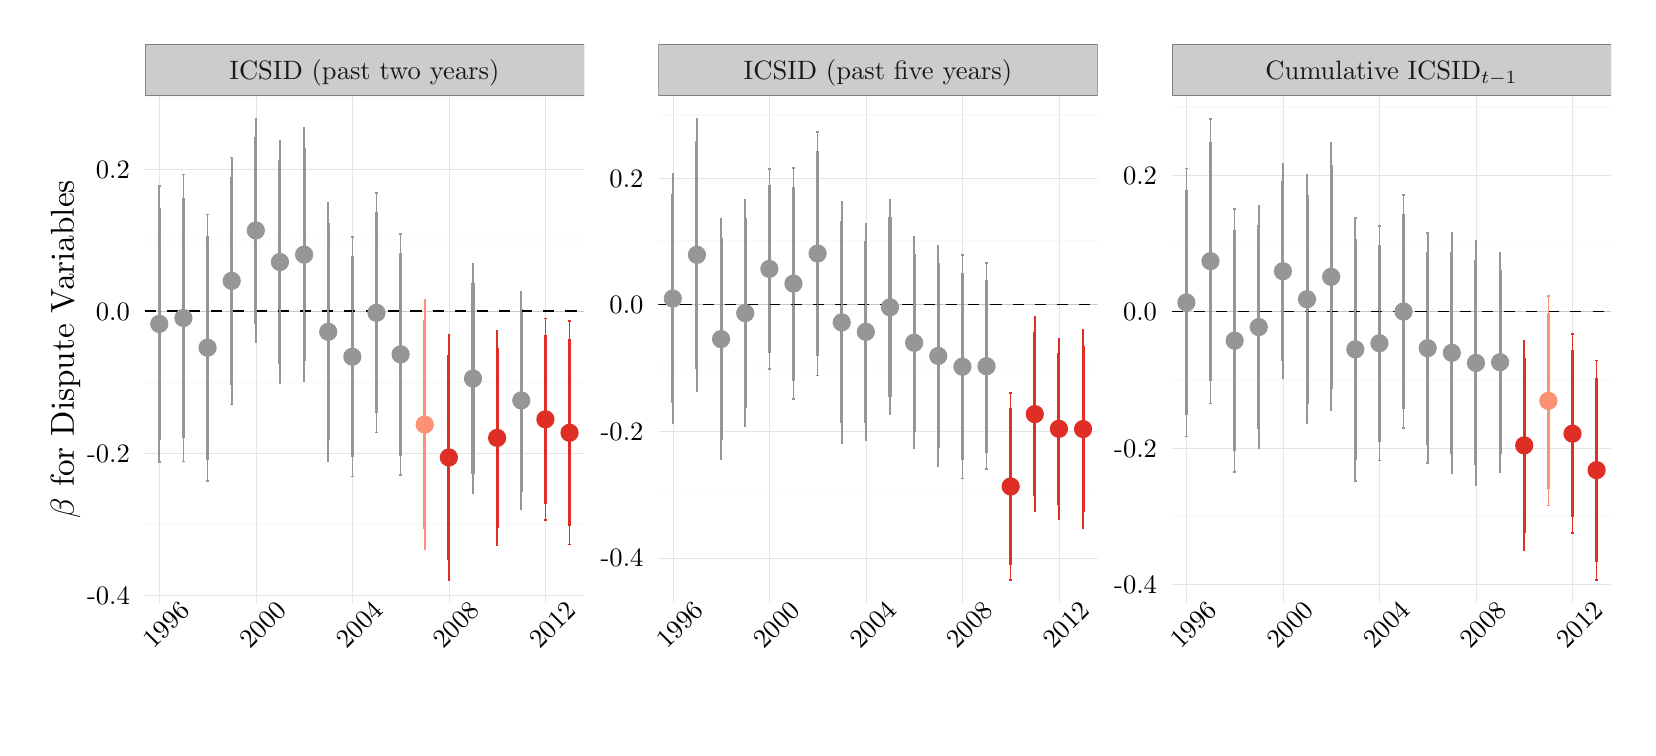
\begin{tikzpicture}[x=1pt,y=1pt]
\definecolor[named]{drawColor}{rgb}{0.00,0.00,0.00}
\definecolor[named]{fillColor}{rgb}{1.00,1.00,1.00}
\fill[color=fillColor,] (0,0) rectangle (578.16,252.94);
\begin{scope}
\path[clip] (  0.00,  0.00) rectangle (578.16,252.94);
\end{scope}
\begin{scope}
\path[clip] (  0.00,  0.00) rectangle (578.16,252.94);
\end{scope}
\begin{scope}
\path[clip] (  0.00,  0.00) rectangle (578.16,252.94);
\end{scope}
\begin{scope}
\path[clip] (  0.00,  0.00) rectangle (578.16,252.94);
\end{scope}
\begin{scope}
\path[clip] (  0.00,  0.00) rectangle (578.16,252.94);
\end{scope}
\begin{scope}
\path[clip] (  0.00,  0.00) rectangle (578.16,252.94);
\end{scope}
\begin{scope}
\path[clip] (  0.00,  0.00) rectangle (578.16,252.94);
\end{scope}
\begin{scope}
\path[clip] (  0.00,  0.00) rectangle (578.16,252.94);
\end{scope}
\begin{scope}
\path[clip] (  0.00,  0.00) rectangle (578.16,252.94);
\end{scope}
\begin{scope}
\path[clip] (  0.00,  0.00) rectangle (578.16,252.94);
\end{scope}
\begin{scope}
\path[clip] (  0.00,  0.00) rectangle (578.16,252.94);
\end{scope}
\begin{scope}
\path[clip] (  0.00,  0.00) rectangle (578.16,252.94);
\end{scope}
\begin{scope}
\path[clip] (  0.00,  0.00) rectangle (578.16,252.94);
\end{scope}
\begin{scope}
\path[clip] (  0.00,  0.00) rectangle (578.16,252.94);
\end{scope}
\begin{scope}
\path[clip] (  0.00,  0.00) rectangle (578.16,252.94);
\end{scope}
\begin{scope}
\path[clip] (  0.00,  0.00) rectangle (578.16,252.94);
\end{scope}
\begin{scope}
\path[clip] (  0.00,  0.00) rectangle (578.16,252.94);
\end{scope}
\begin{scope}
\path[clip] (  0.00,  0.00) rectangle (578.16,252.94);
\end{scope}
\begin{scope}
\path[clip] (  0.00,  0.00) rectangle (578.16,252.94);
\definecolor[named]{drawColor}{rgb}{1.00,1.00,1.00}
\definecolor[named]{fillColor}{rgb}{1.00,1.00,1.00}

\draw[color=drawColor,line width= 0.6pt,line cap=round,line join=round,fill=fillColor,] ( -0.00,  0.00) rectangle (578.16,252.94);
\end{scope}
\begin{scope}
\path[clip] (  0.00,  0.00) rectangle (578.16,252.94);
\end{scope}
\begin{scope}
\path[clip] ( 42.33, 45.11) rectangle (201.03,228.33);
\definecolor[named]{fillColor}{rgb}{1.00,1.00,1.00}

\draw[fill=fillColor,draw opacity=0.00,] ( 42.33, 45.11) rectangle (201.03,228.33);
\definecolor[named]{drawColor}{rgb}{0.98,0.98,0.98}

\draw[color=drawColor,line width= 0.6pt,line join=round,fill opacity=0.00,] ( 42.33, 73.50) --
	(201.03, 73.50);

\draw[color=drawColor,line width= 0.6pt,line join=round,fill opacity=0.00,] ( 42.33,124.81) --
	(201.03,124.81);

\draw[color=drawColor,line width= 0.6pt,line join=round,fill opacity=0.00,] ( 42.33,176.13) --
	(201.03,176.13);

\draw[color=drawColor,line width= 0.6pt,line join=round,fill opacity=0.00,] ( 42.33,227.44) --
	(201.03,227.44);
\definecolor[named]{drawColor}{rgb}{0.90,0.90,0.90}

\draw[color=drawColor,line width= 0.2pt,line join=round,fill opacity=0.00,] ( 42.33, 47.84) --
	(201.03, 47.84);

\draw[color=drawColor,line width= 0.2pt,line join=round,fill opacity=0.00,] ( 42.33, 99.15) --
	(201.03, 99.15);

\draw[color=drawColor,line width= 0.2pt,line join=round,fill opacity=0.00,] ( 42.33,150.47) --
	(201.03,150.47);

\draw[color=drawColor,line width= 0.2pt,line join=round,fill opacity=0.00,] ( 42.33,201.78) --
	(201.03,201.78);

\draw[color=drawColor,line width= 0.2pt,line join=round,fill opacity=0.00,] ( 47.56, 45.11) --
	( 47.56,228.33);

\draw[color=drawColor,line width= 0.2pt,line join=round,fill opacity=0.00,] ( 82.44, 45.11) --
	( 82.44,228.33);

\draw[color=drawColor,line width= 0.2pt,line join=round,fill opacity=0.00,] (117.32, 45.11) --
	(117.32,228.33);

\draw[color=drawColor,line width= 0.2pt,line join=round,fill opacity=0.00,] (152.20, 45.11) --
	(152.20,228.33);

\draw[color=drawColor,line width= 0.2pt,line join=round,fill opacity=0.00,] (187.08, 45.11) --
	(187.08,228.33);
\definecolor[named]{drawColor}{rgb}{0.59,0.59,0.59}
\definecolor[named]{fillColor}{rgb}{0.59,0.59,0.59}

\draw[color=drawColor,line width= 0.3pt,line join=round,fill=fillColor,fill opacity=0.30,draw opacity=0.30,] ( 47.56, 96.06) -- ( 47.56,195.73);

\draw[color=drawColor,line width= 0.3pt,line join=round,fill=fillColor,fill opacity=0.30,draw opacity=0.30,] ( 56.28, 96.18) -- ( 56.28,199.86);

\draw[color=drawColor,line width= 0.3pt,line join=round,fill=fillColor,fill opacity=0.30,draw opacity=0.30,] ( 65.00, 89.13) -- ( 65.00,185.46);

\draw[color=drawColor,line width= 0.3pt,line join=round,fill=fillColor,fill opacity=0.30,draw opacity=0.30,] ( 73.72,116.81) -- ( 73.72,206.08);

\draw[color=drawColor,line width= 0.3pt,line join=round,fill=fillColor,fill opacity=0.30,draw opacity=0.30,] ( 82.44,139.36) -- ( 82.44,220.01);

\draw[color=drawColor,line width= 0.3pt,line join=round,fill=fillColor,fill opacity=0.30,draw opacity=0.30,] ( 91.16,124.31) -- ( 91.16,212.21);

\draw[color=drawColor,line width= 0.3pt,line join=round,fill=fillColor,fill opacity=0.30,draw opacity=0.30,] ( 99.88,125.06) -- ( 99.88,216.79);

\draw[color=drawColor,line width= 0.3pt,line join=round,fill=fillColor,fill opacity=0.30,draw opacity=0.30,] (108.60, 96.32) -- (108.60,189.76);

\draw[color=drawColor,line width= 0.3pt,line join=round,fill=fillColor,fill opacity=0.30,draw opacity=0.30,] (117.32, 90.80) -- (117.32,177.26);

\draw[color=drawColor,line width= 0.3pt,line join=round,fill=fillColor,fill opacity=0.30,draw opacity=0.30,] (126.04,106.67) -- (126.04,193.12);

\draw[color=drawColor,line width= 0.3pt,line join=round,fill=fillColor,fill opacity=0.30,draw opacity=0.30,] (134.76, 91.27) -- (134.76,178.50);
\definecolor[named]{drawColor}{rgb}{0.99,0.57,0.45}
\definecolor[named]{fillColor}{rgb}{0.99,0.57,0.45}

\draw[color=drawColor,line width= 0.3pt,line join=round,fill=fillColor,fill opacity=0.30,draw opacity=0.30,] (143.48, 64.36) -- (143.48,154.69);
\definecolor[named]{drawColor}{rgb}{0.87,0.18,0.15}
\definecolor[named]{fillColor}{rgb}{0.87,0.18,0.15}

\draw[color=drawColor,line width= 0.3pt,line join=round,fill=fillColor,fill opacity=0.30,draw opacity=0.30,] (152.20, 53.44) -- (152.20,141.81);
\definecolor[named]{drawColor}{rgb}{0.59,0.59,0.59}
\definecolor[named]{fillColor}{rgb}{0.59,0.59,0.59}

\draw[color=drawColor,line width= 0.3pt,line join=round,fill=fillColor,fill opacity=0.30,draw opacity=0.30,] (160.92, 84.84) -- (160.92,167.44);
\definecolor[named]{drawColor}{rgb}{0.87,0.18,0.15}
\definecolor[named]{fillColor}{rgb}{0.87,0.18,0.15}

\draw[color=drawColor,line width= 0.3pt,line join=round,fill=fillColor,fill opacity=0.30,draw opacity=0.30,] (169.64, 65.95) -- (169.64,143.45);
\definecolor[named]{drawColor}{rgb}{0.59,0.59,0.59}
\definecolor[named]{fillColor}{rgb}{0.59,0.59,0.59}

\draw[color=drawColor,line width= 0.3pt,line join=round,fill=fillColor,fill opacity=0.30,draw opacity=0.30,] (178.36, 78.96) -- (178.36,157.52);
\definecolor[named]{drawColor}{rgb}{0.87,0.18,0.15}
\definecolor[named]{fillColor}{rgb}{0.87,0.18,0.15}

\draw[color=drawColor,line width= 0.3pt,line join=round,fill=fillColor,fill opacity=0.30,draw opacity=0.30,] (187.08, 74.93) -- (187.08,147.88);

\draw[color=drawColor,line width= 0.3pt,line join=round,fill=fillColor,fill opacity=0.30,draw opacity=0.30,] (195.80, 66.20) -- (195.80,146.91);
\definecolor[named]{drawColor}{rgb}{0.59,0.59,0.59}
\definecolor[named]{fillColor}{rgb}{0.59,0.59,0.59}

\draw[color=drawColor,line width= 1.1pt,line join=round,fill=fillColor,] ( 47.56,104.07) -- ( 47.56,187.72);

\draw[color=drawColor,line width= 1.1pt,line join=round,fill=fillColor,] ( 56.28,104.51) -- ( 56.28,191.52);

\draw[color=drawColor,line width= 1.1pt,line join=round,fill=fillColor,] ( 65.00, 96.88) -- ( 65.00,177.71);

\draw[color=drawColor,line width= 1.1pt,line join=round,fill=fillColor,] ( 73.72,123.99) -- ( 73.72,198.91);

\draw[color=drawColor,line width= 1.1pt,line join=round,fill=fillColor,] ( 82.44,145.84) -- ( 82.44,213.52);

\draw[color=drawColor,line width= 1.1pt,line join=round,fill=fillColor,] ( 91.16,131.38) -- ( 91.16,205.14);

\draw[color=drawColor,line width= 1.1pt,line join=round,fill=fillColor,] ( 99.88,132.44) -- ( 99.88,209.42);

\draw[color=drawColor,line width= 1.1pt,line join=round,fill=fillColor,] (108.60,103.83) -- (108.60,182.25);

\draw[color=drawColor,line width= 1.1pt,line join=round,fill=fillColor,] (117.32, 97.75) -- (117.32,170.31);

\draw[color=drawColor,line width= 1.1pt,line join=round,fill=fillColor,] (126.04,113.62) -- (126.04,186.17);

\draw[color=drawColor,line width= 1.1pt,line join=round,fill=fillColor,] (134.76, 98.28) -- (134.76,171.49);
\definecolor[named]{drawColor}{rgb}{0.99,0.57,0.45}
\definecolor[named]{fillColor}{rgb}{0.99,0.57,0.45}

\draw[color=drawColor,line width= 1.1pt,line join=round,fill=fillColor,] (143.48, 71.62) -- (143.48,147.43);
\definecolor[named]{drawColor}{rgb}{0.87,0.18,0.15}
\definecolor[named]{fillColor}{rgb}{0.87,0.18,0.15}

\draw[color=drawColor,line width= 1.1pt,line join=round,fill=fillColor,] (152.20, 60.55) -- (152.20,134.71);
\definecolor[named]{drawColor}{rgb}{0.59,0.59,0.59}
\definecolor[named]{fillColor}{rgb}{0.59,0.59,0.59}

\draw[color=drawColor,line width= 1.1pt,line join=round,fill=fillColor,] (160.92, 91.48) -- (160.92,160.80);
\definecolor[named]{drawColor}{rgb}{0.87,0.18,0.15}
\definecolor[named]{fillColor}{rgb}{0.87,0.18,0.15}

\draw[color=drawColor,line width= 1.1pt,line join=round,fill=fillColor,] (169.64, 72.18) -- (169.64,137.22);
\definecolor[named]{drawColor}{rgb}{0.59,0.59,0.59}
\definecolor[named]{fillColor}{rgb}{0.59,0.59,0.59}

\draw[color=drawColor,line width= 1.1pt,line join=round,fill=fillColor,] (178.36, 85.28) -- (178.36,151.20);
\definecolor[named]{drawColor}{rgb}{0.87,0.18,0.15}
\definecolor[named]{fillColor}{rgb}{0.87,0.18,0.15}

\draw[color=drawColor,line width= 1.1pt,line join=round,fill=fillColor,] (187.08, 80.80) -- (187.08,142.02);

\draw[color=drawColor,line width= 1.1pt,line join=round,fill=fillColor,] (195.80, 72.69) -- (195.80,140.42);
\definecolor[named]{drawColor}{rgb}{0.00,0.00,0.00}
\definecolor[named]{fillColor}{rgb}{0.00,0.00,0.00}

\draw[color=drawColor,line width= 0.6pt,dash pattern=on 4pt off 4pt ,line join=round,fill=fillColor,] ( 42.33,150.47) -- (201.03,150.47);
\definecolor[named]{drawColor}{rgb}{0.59,0.59,0.59}
\definecolor[named]{fillColor}{rgb}{0.59,0.59,0.59}

\draw[color=drawColor,line width= 0.4pt,line cap=round,line join=round,fill=fillColor,] ( 47.56,145.89) circle (  3.09);

\draw[color=drawColor,line width= 0.4pt,line cap=round,line join=round,fill=fillColor,] ( 56.28,148.02) circle (  3.09);

\draw[color=drawColor,line width= 0.4pt,line cap=round,line join=round,fill=fillColor,] ( 65.00,137.29) circle (  3.09);

\draw[color=drawColor,line width= 0.4pt,line cap=round,line join=round,fill=fillColor,] ( 73.72,161.45) circle (  3.09);

\draw[color=drawColor,line width= 0.4pt,line cap=round,line join=round,fill=fillColor,] ( 82.44,179.68) circle (  3.09);

\draw[color=drawColor,line width= 0.4pt,line cap=round,line join=round,fill=fillColor,] ( 91.16,168.26) circle (  3.09);

\draw[color=drawColor,line width= 0.4pt,line cap=round,line join=round,fill=fillColor,] ( 99.88,170.93) circle (  3.09);

\draw[color=drawColor,line width= 0.4pt,line cap=round,line join=round,fill=fillColor,] (108.60,143.04) circle (  3.09);

\draw[color=drawColor,line width= 0.4pt,line cap=round,line join=round,fill=fillColor,] (117.32,134.03) circle (  3.09);

\draw[color=drawColor,line width= 0.4pt,line cap=round,line join=round,fill=fillColor,] (126.04,149.90) circle (  3.09);

\draw[color=drawColor,line width= 0.4pt,line cap=round,line join=round,fill=fillColor,] (134.76,134.89) circle (  3.09);
\definecolor[named]{drawColor}{rgb}{0.99,0.57,0.45}
\definecolor[named]{fillColor}{rgb}{0.99,0.57,0.45}

\draw[color=drawColor,line width= 0.4pt,line cap=round,line join=round,fill=fillColor,] (143.48,109.52) circle (  3.09);
\definecolor[named]{drawColor}{rgb}{0.87,0.18,0.15}
\definecolor[named]{fillColor}{rgb}{0.87,0.18,0.15}

\draw[color=drawColor,line width= 0.4pt,line cap=round,line join=round,fill=fillColor,] (152.20, 97.63) circle (  3.09);
\definecolor[named]{drawColor}{rgb}{0.59,0.59,0.59}
\definecolor[named]{fillColor}{rgb}{0.59,0.59,0.59}

\draw[color=drawColor,line width= 0.4pt,line cap=round,line join=round,fill=fillColor,] (160.92,126.14) circle (  3.09);
\definecolor[named]{drawColor}{rgb}{0.87,0.18,0.15}
\definecolor[named]{fillColor}{rgb}{0.87,0.18,0.15}

\draw[color=drawColor,line width= 0.4pt,line cap=round,line join=round,fill=fillColor,] (169.64,104.70) circle (  3.09);
\definecolor[named]{drawColor}{rgb}{0.59,0.59,0.59}
\definecolor[named]{fillColor}{rgb}{0.59,0.59,0.59}

\draw[color=drawColor,line width= 0.4pt,line cap=round,line join=round,fill=fillColor,] (178.36,118.24) circle (  3.09);
\definecolor[named]{drawColor}{rgb}{0.87,0.18,0.15}
\definecolor[named]{fillColor}{rgb}{0.87,0.18,0.15}

\draw[color=drawColor,line width= 0.4pt,line cap=round,line join=round,fill=fillColor,] (187.08,111.41) circle (  3.09);

\draw[color=drawColor,line width= 0.4pt,line cap=round,line join=round,fill=fillColor,] (195.80,106.55) circle (  3.09);
\definecolor[named]{drawColor}{rgb}{0.59,0.59,0.59}
\definecolor[named]{fillColor}{rgb}{0.59,0.59,0.59}

\draw[color=drawColor,line width= 0.6pt,line join=round,] ( 47.12,195.73) --
	( 48.00,195.73);

\draw[color=drawColor,line width= 0.6pt,line join=round,] ( 47.56,195.73) --
	( 47.56, 96.06);

\draw[color=drawColor,line width= 0.6pt,line join=round,] ( 47.12, 96.06) --
	( 48.00, 96.06);

\draw[color=drawColor,line width= 0.6pt,line join=round,] ( 55.84,199.86) --
	( 56.72,199.86);

\draw[color=drawColor,line width= 0.6pt,line join=round,] ( 56.28,199.86) --
	( 56.28, 96.18);

\draw[color=drawColor,line width= 0.6pt,line join=round,] ( 55.84, 96.18) --
	( 56.72, 96.18);

\draw[color=drawColor,line width= 0.6pt,line join=round,] ( 64.56,185.46) --
	( 65.44,185.46);

\draw[color=drawColor,line width= 0.6pt,line join=round,] ( 65.00,185.46) --
	( 65.00, 89.13);

\draw[color=drawColor,line width= 0.6pt,line join=round,] ( 64.56, 89.13) --
	( 65.44, 89.13);

\draw[color=drawColor,line width= 0.6pt,line join=round,] ( 73.28,206.08) --
	( 74.16,206.08);

\draw[color=drawColor,line width= 0.6pt,line join=round,] ( 73.72,206.08) --
	( 73.72,116.81);

\draw[color=drawColor,line width= 0.6pt,line join=round,] ( 73.28,116.81) --
	( 74.16,116.81);

\draw[color=drawColor,line width= 0.6pt,line join=round,] ( 82.00,220.01) --
	( 82.88,220.01);

\draw[color=drawColor,line width= 0.6pt,line join=round,] ( 82.44,220.01) --
	( 82.44,139.36);

\draw[color=drawColor,line width= 0.6pt,line join=round,] ( 82.00,139.36) --
	( 82.88,139.36);

\draw[color=drawColor,line width= 0.6pt,line join=round,] ( 90.72,212.21) --
	( 91.60,212.21);

\draw[color=drawColor,line width= 0.6pt,line join=round,] ( 91.16,212.21) --
	( 91.16,124.31);

\draw[color=drawColor,line width= 0.6pt,line join=round,] ( 90.72,124.31) --
	( 91.60,124.31);

\draw[color=drawColor,line width= 0.6pt,line join=round,] ( 99.44,216.79) --
	(100.31,216.79);

\draw[color=drawColor,line width= 0.6pt,line join=round,] ( 99.88,216.79) --
	( 99.88,125.06);

\draw[color=drawColor,line width= 0.6pt,line join=round,] ( 99.44,125.06) --
	(100.31,125.06);

\draw[color=drawColor,line width= 0.6pt,line join=round,] (108.16,189.76) --
	(109.03,189.76);

\draw[color=drawColor,line width= 0.6pt,line join=round,] (108.60,189.76) --
	(108.60, 96.32);

\draw[color=drawColor,line width= 0.6pt,line join=round,] (108.16, 96.32) --
	(109.03, 96.32);

\draw[color=drawColor,line width= 0.6pt,line join=round,] (116.88,177.26) --
	(117.75,177.26);

\draw[color=drawColor,line width= 0.6pt,line join=round,] (117.32,177.26) --
	(117.32, 90.80);

\draw[color=drawColor,line width= 0.6pt,line join=round,] (116.88, 90.80) --
	(117.75, 90.80);

\draw[color=drawColor,line width= 0.6pt,line join=round,] (125.60,193.12) --
	(126.47,193.12);

\draw[color=drawColor,line width= 0.6pt,line join=round,] (126.04,193.12) --
	(126.04,106.67);

\draw[color=drawColor,line width= 0.6pt,line join=round,] (125.60,106.67) --
	(126.47,106.67);

\draw[color=drawColor,line width= 0.6pt,line join=round,] (134.32,178.50) --
	(135.19,178.50);

\draw[color=drawColor,line width= 0.6pt,line join=round,] (134.76,178.50) --
	(134.76, 91.27);

\draw[color=drawColor,line width= 0.6pt,line join=round,] (134.32, 91.27) --
	(135.19, 91.27);
\definecolor[named]{drawColor}{rgb}{0.99,0.57,0.45}
\definecolor[named]{fillColor}{rgb}{0.99,0.57,0.45}

\draw[color=drawColor,line width= 0.6pt,line join=round,] (143.04,154.69) --
	(143.91,154.69);

\draw[color=drawColor,line width= 0.6pt,line join=round,] (143.48,154.69) --
	(143.48, 64.36);

\draw[color=drawColor,line width= 0.6pt,line join=round,] (143.04, 64.36) --
	(143.91, 64.36);
\definecolor[named]{drawColor}{rgb}{0.87,0.18,0.15}
\definecolor[named]{fillColor}{rgb}{0.87,0.18,0.15}

\draw[color=drawColor,line width= 0.6pt,line join=round,] (151.76,141.81) --
	(152.63,141.81);

\draw[color=drawColor,line width= 0.6pt,line join=round,] (152.20,141.81) --
	(152.20, 53.44);

\draw[color=drawColor,line width= 0.6pt,line join=round,] (151.76, 53.44) --
	(152.63, 53.44);
\definecolor[named]{drawColor}{rgb}{0.59,0.59,0.59}
\definecolor[named]{fillColor}{rgb}{0.59,0.59,0.59}

\draw[color=drawColor,line width= 0.6pt,line join=round,] (160.48,167.44) --
	(161.35,167.44);

\draw[color=drawColor,line width= 0.6pt,line join=round,] (160.92,167.44) --
	(160.92, 84.84);

\draw[color=drawColor,line width= 0.6pt,line join=round,] (160.48, 84.84) --
	(161.35, 84.84);
\definecolor[named]{drawColor}{rgb}{0.87,0.18,0.15}
\definecolor[named]{fillColor}{rgb}{0.87,0.18,0.15}

\draw[color=drawColor,line width= 0.6pt,line join=round,] (169.20,143.45) --
	(170.07,143.45);

\draw[color=drawColor,line width= 0.6pt,line join=round,] (169.64,143.45) --
	(169.64, 65.95);

\draw[color=drawColor,line width= 0.6pt,line join=round,] (169.20, 65.95) --
	(170.07, 65.95);
\definecolor[named]{drawColor}{rgb}{0.59,0.59,0.59}
\definecolor[named]{fillColor}{rgb}{0.59,0.59,0.59}

\draw[color=drawColor,line width= 0.6pt,line join=round,] (177.92,157.52) --
	(178.79,157.52);

\draw[color=drawColor,line width= 0.6pt,line join=round,] (178.36,157.52) --
	(178.36, 78.96);

\draw[color=drawColor,line width= 0.6pt,line join=round,] (177.92, 78.96) --
	(178.79, 78.96);
\definecolor[named]{drawColor}{rgb}{0.87,0.18,0.15}
\definecolor[named]{fillColor}{rgb}{0.87,0.18,0.15}

\draw[color=drawColor,line width= 0.6pt,line join=round,] (186.64,147.88) --
	(187.51,147.88);

\draw[color=drawColor,line width= 0.6pt,line join=round,] (187.08,147.88) --
	(187.08, 74.93);

\draw[color=drawColor,line width= 0.6pt,line join=round,] (186.64, 74.93) --
	(187.51, 74.93);

\draw[color=drawColor,line width= 0.6pt,line join=round,] (195.36,146.91) --
	(196.23,146.91);

\draw[color=drawColor,line width= 0.6pt,line join=round,] (195.80,146.91) --
	(195.80, 66.20);

\draw[color=drawColor,line width= 0.6pt,line join=round,] (195.36, 66.20) --
	(196.23, 66.20);
\end{scope}
\begin{scope}
\path[clip] (  0.00,  0.00) rectangle (578.16,252.94);
\end{scope}
\begin{scope}
\path[clip] (227.89, 45.11) rectangle (386.59,228.33);
\definecolor[named]{fillColor}{rgb}{1.00,1.00,1.00}

\draw[fill=fillColor,draw opacity=0.00,] (227.89, 45.11) rectangle (386.59,228.33);
\definecolor[named]{drawColor}{rgb}{0.98,0.98,0.98}

\draw[color=drawColor,line width= 0.6pt,line join=round,fill opacity=0.00,] (227.89, 84.26) --
	(386.59, 84.26);

\draw[color=drawColor,line width= 0.6pt,line join=round,fill opacity=0.00,] (227.89,130.00) --
	(386.59,130.00);

\draw[color=drawColor,line width= 0.6pt,line join=round,fill opacity=0.00,] (227.89,175.75) --
	(386.59,175.75);

\draw[color=drawColor,line width= 0.6pt,line join=round,fill opacity=0.00,] (227.89,221.49) --
	(386.59,221.49);
\definecolor[named]{drawColor}{rgb}{0.90,0.90,0.90}

\draw[color=drawColor,line width= 0.2pt,line join=round,fill opacity=0.00,] (227.89, 61.38) --
	(386.59, 61.38);

\draw[color=drawColor,line width= 0.2pt,line join=round,fill opacity=0.00,] (227.89,107.13) --
	(386.59,107.13);

\draw[color=drawColor,line width= 0.2pt,line join=round,fill opacity=0.00,] (227.89,152.87) --
	(386.59,152.87);

\draw[color=drawColor,line width= 0.2pt,line join=round,fill opacity=0.00,] (227.89,198.62) --
	(386.59,198.62);

\draw[color=drawColor,line width= 0.2pt,line join=round,fill opacity=0.00,] (233.12, 45.11) --
	(233.12,228.33);

\draw[color=drawColor,line width= 0.2pt,line join=round,fill opacity=0.00,] (268.00, 45.11) --
	(268.00,228.33);

\draw[color=drawColor,line width= 0.2pt,line join=round,fill opacity=0.00,] (302.88, 45.11) --
	(302.88,228.33);

\draw[color=drawColor,line width= 0.2pt,line join=round,fill opacity=0.00,] (337.76, 45.11) --
	(337.76,228.33);

\draw[color=drawColor,line width= 0.2pt,line join=round,fill opacity=0.00,] (372.64, 45.11) --
	(372.64,228.33);
\definecolor[named]{drawColor}{rgb}{0.59,0.59,0.59}
\definecolor[named]{fillColor}{rgb}{0.59,0.59,0.59}

\draw[color=drawColor,line width= 0.3pt,line join=round,fill=fillColor,fill opacity=0.30,draw opacity=0.30,] (233.12,109.97) -- (233.12,200.12);

\draw[color=drawColor,line width= 0.3pt,line join=round,fill=fillColor,fill opacity=0.30,draw opacity=0.30,] (241.84,121.71) -- (241.84,220.01);

\draw[color=drawColor,line width= 0.3pt,line join=round,fill=fillColor,fill opacity=0.30,draw opacity=0.30,] (250.56, 96.93) -- (250.56,183.88);

\draw[color=drawColor,line width= 0.3pt,line join=round,fill=fillColor,fill opacity=0.30,draw opacity=0.30,] (259.28,108.99) -- (259.28,190.62);

\draw[color=drawColor,line width= 0.3pt,line join=round,fill=fillColor,fill opacity=0.30,draw opacity=0.30,] (268.00,129.62) -- (268.00,201.92);

\draw[color=drawColor,line width= 0.3pt,line join=round,fill=fillColor,fill opacity=0.30,draw opacity=0.30,] (276.72,118.73) -- (276.72,202.16);

\draw[color=drawColor,line width= 0.3pt,line join=round,fill=fillColor,fill opacity=0.30,draw opacity=0.30,] (285.44,127.30) -- (285.44,215.35);

\draw[color=drawColor,line width= 0.3pt,line join=round,fill=fillColor,fill opacity=0.30,draw opacity=0.30,] (294.16,102.93) -- (294.16,189.95);

\draw[color=drawColor,line width= 0.3pt,line join=round,fill=fillColor,fill opacity=0.30,draw opacity=0.30,] (302.88,103.98) -- (302.88,182.08);

\draw[color=drawColor,line width= 0.3pt,line join=round,fill=fillColor,fill opacity=0.30,draw opacity=0.30,] (311.60,113.17) -- (311.60,190.58);

\draw[color=drawColor,line width= 0.3pt,line join=round,fill=fillColor,fill opacity=0.30,draw opacity=0.30,] (320.32,100.85) -- (320.32,177.30);

\draw[color=drawColor,line width= 0.3pt,line join=round,fill=fillColor,fill opacity=0.30,draw opacity=0.30,] (329.04, 94.51) -- (329.04,174.13);

\draw[color=drawColor,line width= 0.3pt,line join=round,fill=fillColor,fill opacity=0.30,draw opacity=0.30,] (337.76, 90.08) -- (337.76,170.78);

\draw[color=drawColor,line width= 0.3pt,line join=round,fill=fillColor,fill opacity=0.30,draw opacity=0.30,] (346.48, 93.42) -- (346.48,167.79);
\definecolor[named]{drawColor}{rgb}{0.87,0.18,0.15}
\definecolor[named]{fillColor}{rgb}{0.87,0.18,0.15}

\draw[color=drawColor,line width= 0.3pt,line join=round,fill=fillColor,fill opacity=0.30,draw opacity=0.30,] (355.20, 53.44) -- (355.20,120.86);

\draw[color=drawColor,line width= 0.3pt,line join=round,fill=fillColor,fill opacity=0.30,draw opacity=0.30,] (363.92, 78.07) -- (363.92,148.53);

\draw[color=drawColor,line width= 0.3pt,line join=round,fill=fillColor,fill opacity=0.30,draw opacity=0.30,] (372.64, 75.36) -- (372.64,140.63);

\draw[color=drawColor,line width= 0.3pt,line join=round,fill=fillColor,fill opacity=0.30,draw opacity=0.30,] (381.36, 72.13) -- (381.36,143.68);
\definecolor[named]{drawColor}{rgb}{0.59,0.59,0.59}
\definecolor[named]{fillColor}{rgb}{0.59,0.59,0.59}

\draw[color=drawColor,line width= 1.1pt,line join=round,fill=fillColor,] (233.12,117.22) -- (233.12,192.88);

\draw[color=drawColor,line width= 1.1pt,line join=round,fill=fillColor,] (241.84,129.61) -- (241.84,212.10);

\draw[color=drawColor,line width= 1.1pt,line join=round,fill=fillColor,] (250.56,103.92) -- (250.56,176.89);

\draw[color=drawColor,line width= 1.1pt,line join=round,fill=fillColor,] (259.28,115.55) -- (259.28,184.05);

\draw[color=drawColor,line width= 1.1pt,line join=round,fill=fillColor,] (268.00,135.44) -- (268.00,196.11);

\draw[color=drawColor,line width= 1.1pt,line join=round,fill=fillColor,] (276.72,125.43) -- (276.72,195.46);

\draw[color=drawColor,line width= 1.1pt,line join=round,fill=fillColor,] (285.44,134.38) -- (285.44,208.27);

\draw[color=drawColor,line width= 1.1pt,line join=round,fill=fillColor,] (294.16,109.93) -- (294.16,182.95);

\draw[color=drawColor,line width= 1.1pt,line join=round,fill=fillColor,] (302.88,110.26) -- (302.88,175.80);

\draw[color=drawColor,line width= 1.1pt,line join=round,fill=fillColor,] (311.60,119.39) -- (311.60,184.36);

\draw[color=drawColor,line width= 1.1pt,line join=round,fill=fillColor,] (320.32,107.00) -- (320.32,171.16);

\draw[color=drawColor,line width= 1.1pt,line join=round,fill=fillColor,] (329.04,100.91) -- (329.04,167.73);

\draw[color=drawColor,line width= 1.1pt,line join=round,fill=fillColor,] (337.76, 96.57) -- (337.76,164.29);

\draw[color=drawColor,line width= 1.1pt,line join=round,fill=fillColor,] (346.48, 99.40) -- (346.48,161.81);
\definecolor[named]{drawColor}{rgb}{0.87,0.18,0.15}
\definecolor[named]{fillColor}{rgb}{0.87,0.18,0.15}

\draw[color=drawColor,line width= 1.1pt,line join=round,fill=fillColor,] (355.20, 58.86) -- (355.20,115.44);

\draw[color=drawColor,line width= 1.1pt,line join=round,fill=fillColor,] (363.92, 83.74) -- (363.92,142.86);

\draw[color=drawColor,line width= 1.1pt,line join=round,fill=fillColor,] (372.64, 80.61) -- (372.64,135.38);

\draw[color=drawColor,line width= 1.1pt,line join=round,fill=fillColor,] (381.36, 77.88) -- (381.36,137.93);
\definecolor[named]{drawColor}{rgb}{0.00,0.00,0.00}
\definecolor[named]{fillColor}{rgb}{0.00,0.00,0.00}

\draw[color=drawColor,line width= 0.6pt,dash pattern=on 4pt off 4pt ,line join=round,fill=fillColor,] (227.89,152.87) -- (386.59,152.87);
\definecolor[named]{drawColor}{rgb}{0.59,0.59,0.59}
\definecolor[named]{fillColor}{rgb}{0.59,0.59,0.59}

\draw[color=drawColor,line width= 0.4pt,line cap=round,line join=round,fill=fillColor,] (233.12,155.05) circle (  3.09);

\draw[color=drawColor,line width= 0.4pt,line cap=round,line join=round,fill=fillColor,] (241.84,170.86) circle (  3.09);

\draw[color=drawColor,line width= 0.4pt,line cap=round,line join=round,fill=fillColor,] (250.56,140.40) circle (  3.09);

\draw[color=drawColor,line width= 0.4pt,line cap=round,line join=round,fill=fillColor,] (259.28,149.80) circle (  3.09);

\draw[color=drawColor,line width= 0.4pt,line cap=round,line join=round,fill=fillColor,] (268.00,165.77) circle (  3.09);

\draw[color=drawColor,line width= 0.4pt,line cap=round,line join=round,fill=fillColor,] (276.72,160.45) circle (  3.09);

\draw[color=drawColor,line width= 0.4pt,line cap=round,line join=round,fill=fillColor,] (285.44,171.33) circle (  3.09);

\draw[color=drawColor,line width= 0.4pt,line cap=round,line join=round,fill=fillColor,] (294.16,146.44) circle (  3.09);

\draw[color=drawColor,line width= 0.4pt,line cap=round,line join=round,fill=fillColor,] (302.88,143.03) circle (  3.09);

\draw[color=drawColor,line width= 0.4pt,line cap=round,line join=round,fill=fillColor,] (311.60,151.88) circle (  3.09);

\draw[color=drawColor,line width= 0.4pt,line cap=round,line join=round,fill=fillColor,] (320.32,139.08) circle (  3.09);

\draw[color=drawColor,line width= 0.4pt,line cap=round,line join=round,fill=fillColor,] (329.04,134.32) circle (  3.09);

\draw[color=drawColor,line width= 0.4pt,line cap=round,line join=round,fill=fillColor,] (337.76,130.43) circle (  3.09);

\draw[color=drawColor,line width= 0.4pt,line cap=round,line join=round,fill=fillColor,] (346.48,130.61) circle (  3.09);
\definecolor[named]{drawColor}{rgb}{0.87,0.18,0.15}
\definecolor[named]{fillColor}{rgb}{0.87,0.18,0.15}

\draw[color=drawColor,line width= 0.4pt,line cap=round,line join=round,fill=fillColor,] (355.20, 87.15) circle (  3.09);

\draw[color=drawColor,line width= 0.4pt,line cap=round,line join=round,fill=fillColor,] (363.92,113.30) circle (  3.09);

\draw[color=drawColor,line width= 0.4pt,line cap=round,line join=round,fill=fillColor,] (372.64,107.99) circle (  3.09);

\draw[color=drawColor,line width= 0.4pt,line cap=round,line join=round,fill=fillColor,] (381.36,107.90) circle (  3.09);
\definecolor[named]{drawColor}{rgb}{0.59,0.59,0.59}
\definecolor[named]{fillColor}{rgb}{0.59,0.59,0.59}

\draw[color=drawColor,line width= 0.6pt,line join=round,] (232.69,200.12) --
	(233.56,200.12);

\draw[color=drawColor,line width= 0.6pt,line join=round,] (233.12,200.12) --
	(233.12,109.97);

\draw[color=drawColor,line width= 0.6pt,line join=round,] (232.69,109.97) --
	(233.56,109.97);

\draw[color=drawColor,line width= 0.6pt,line join=round,] (241.41,220.01) --
	(242.28,220.01);

\draw[color=drawColor,line width= 0.6pt,line join=round,] (241.84,220.01) --
	(241.84,121.71);

\draw[color=drawColor,line width= 0.6pt,line join=round,] (241.41,121.71) --
	(242.28,121.71);

\draw[color=drawColor,line width= 0.6pt,line join=round,] (250.13,183.88) --
	(251.00,183.88);

\draw[color=drawColor,line width= 0.6pt,line join=round,] (250.56,183.88) --
	(250.56, 96.93);

\draw[color=drawColor,line width= 0.6pt,line join=round,] (250.13, 96.93) --
	(251.00, 96.93);

\draw[color=drawColor,line width= 0.6pt,line join=round,] (258.85,190.62) --
	(259.72,190.62);

\draw[color=drawColor,line width= 0.6pt,line join=round,] (259.28,190.62) --
	(259.28,108.99);

\draw[color=drawColor,line width= 0.6pt,line join=round,] (258.85,108.99) --
	(259.72,108.99);

\draw[color=drawColor,line width= 0.6pt,line join=round,] (267.57,201.92) --
	(268.44,201.92);

\draw[color=drawColor,line width= 0.6pt,line join=round,] (268.00,201.92) --
	(268.00,129.62);

\draw[color=drawColor,line width= 0.6pt,line join=round,] (267.57,129.62) --
	(268.44,129.62);

\draw[color=drawColor,line width= 0.6pt,line join=round,] (276.29,202.16) --
	(277.16,202.16);

\draw[color=drawColor,line width= 0.6pt,line join=round,] (276.72,202.16) --
	(276.72,118.73);

\draw[color=drawColor,line width= 0.6pt,line join=round,] (276.29,118.73) --
	(277.16,118.73);

\draw[color=drawColor,line width= 0.6pt,line join=round,] (285.01,215.35) --
	(285.88,215.35);

\draw[color=drawColor,line width= 0.6pt,line join=round,] (285.44,215.35) --
	(285.44,127.30);

\draw[color=drawColor,line width= 0.6pt,line join=round,] (285.01,127.30) --
	(285.88,127.30);

\draw[color=drawColor,line width= 0.6pt,line join=round,] (293.73,189.95) --
	(294.60,189.95);

\draw[color=drawColor,line width= 0.6pt,line join=round,] (294.16,189.95) --
	(294.16,102.93);

\draw[color=drawColor,line width= 0.6pt,line join=round,] (293.73,102.93) --
	(294.60,102.93);

\draw[color=drawColor,line width= 0.6pt,line join=round,] (302.45,182.08) --
	(303.32,182.08);

\draw[color=drawColor,line width= 0.6pt,line join=round,] (302.88,182.08) --
	(302.88,103.98);

\draw[color=drawColor,line width= 0.6pt,line join=round,] (302.45,103.98) --
	(303.32,103.98);

\draw[color=drawColor,line width= 0.6pt,line join=round,] (311.17,190.58) --
	(312.04,190.58);

\draw[color=drawColor,line width= 0.6pt,line join=round,] (311.60,190.58) --
	(311.60,113.17);

\draw[color=drawColor,line width= 0.6pt,line join=round,] (311.17,113.17) --
	(312.04,113.17);

\draw[color=drawColor,line width= 0.6pt,line join=round,] (319.89,177.30) --
	(320.76,177.30);

\draw[color=drawColor,line width= 0.6pt,line join=round,] (320.32,177.30) --
	(320.32,100.85);

\draw[color=drawColor,line width= 0.6pt,line join=round,] (319.89,100.85) --
	(320.76,100.85);

\draw[color=drawColor,line width= 0.6pt,line join=round,] (328.61,174.13) --
	(329.48,174.13);

\draw[color=drawColor,line width= 0.6pt,line join=round,] (329.04,174.13) --
	(329.04, 94.51);

\draw[color=drawColor,line width= 0.6pt,line join=round,] (328.61, 94.51) --
	(329.48, 94.51);

\draw[color=drawColor,line width= 0.6pt,line join=round,] (337.33,170.78) --
	(338.20,170.78);

\draw[color=drawColor,line width= 0.6pt,line join=round,] (337.76,170.78) --
	(337.76, 90.08);

\draw[color=drawColor,line width= 0.6pt,line join=round,] (337.33, 90.08) --
	(338.20, 90.08);

\draw[color=drawColor,line width= 0.6pt,line join=round,] (346.05,167.79) --
	(346.92,167.79);

\draw[color=drawColor,line width= 0.6pt,line join=round,] (346.48,167.79) --
	(346.48, 93.42);

\draw[color=drawColor,line width= 0.6pt,line join=round,] (346.05, 93.42) --
	(346.92, 93.42);
\definecolor[named]{drawColor}{rgb}{0.87,0.18,0.15}
\definecolor[named]{fillColor}{rgb}{0.87,0.18,0.15}

\draw[color=drawColor,line width= 0.6pt,line join=round,] (354.77,120.86) --
	(355.64,120.86);

\draw[color=drawColor,line width= 0.6pt,line join=round,] (355.20,120.86) --
	(355.20, 53.44);

\draw[color=drawColor,line width= 0.6pt,line join=round,] (354.77, 53.44) --
	(355.64, 53.44);

\draw[color=drawColor,line width= 0.6pt,line join=round,] (363.49,148.53) --
	(364.36,148.53);

\draw[color=drawColor,line width= 0.6pt,line join=round,] (363.92,148.53) --
	(363.92, 78.07);

\draw[color=drawColor,line width= 0.6pt,line join=round,] (363.49, 78.07) --
	(364.36, 78.07);

\draw[color=drawColor,line width= 0.6pt,line join=round,] (372.21,140.63) --
	(373.08,140.63);

\draw[color=drawColor,line width= 0.6pt,line join=round,] (372.64,140.63) --
	(372.64, 75.36);

\draw[color=drawColor,line width= 0.6pt,line join=round,] (372.21, 75.36) --
	(373.08, 75.36);

\draw[color=drawColor,line width= 0.6pt,line join=round,] (380.93,143.68) --
	(381.80,143.68);

\draw[color=drawColor,line width= 0.6pt,line join=round,] (381.36,143.68) --
	(381.36, 72.13);

\draw[color=drawColor,line width= 0.6pt,line join=round,] (380.93, 72.13) --
	(381.80, 72.13);
\end{scope}
\begin{scope}
\path[clip] (  0.00,  0.00) rectangle (578.16,252.94);
\end{scope}
\begin{scope}
\path[clip] (413.46, 45.11) rectangle (572.16,228.33);
\definecolor[named]{fillColor}{rgb}{1.00,1.00,1.00}

\draw[fill=fillColor,draw opacity=0.00,] (413.46, 45.11) rectangle (572.16,228.33);
\definecolor[named]{drawColor}{rgb}{0.98,0.98,0.98}

\draw[color=drawColor,line width= 0.6pt,line join=round,fill opacity=0.00,] (413.46, 76.44) --
	(572.16, 76.44);

\draw[color=drawColor,line width= 0.6pt,line join=round,fill opacity=0.00,] (413.46,125.72) --
	(572.16,125.72);

\draw[color=drawColor,line width= 0.6pt,line join=round,fill opacity=0.00,] (413.46,175.00) --
	(572.16,175.00);

\draw[color=drawColor,line width= 0.6pt,line join=round,fill opacity=0.00,] (413.46,224.28) --
	(572.16,224.28);
\definecolor[named]{drawColor}{rgb}{0.90,0.90,0.90}

\draw[color=drawColor,line width= 0.2pt,line join=round,fill opacity=0.00,] (413.46, 51.81) --
	(572.16, 51.81);

\draw[color=drawColor,line width= 0.2pt,line join=round,fill opacity=0.00,] (413.46,101.08) --
	(572.16,101.08);

\draw[color=drawColor,line width= 0.2pt,line join=round,fill opacity=0.00,] (413.46,150.36) --
	(572.16,150.36);

\draw[color=drawColor,line width= 0.2pt,line join=round,fill opacity=0.00,] (413.46,199.64) --
	(572.16,199.64);

\draw[color=drawColor,line width= 0.2pt,line join=round,fill opacity=0.00,] (418.69, 45.11) --
	(418.69,228.33);

\draw[color=drawColor,line width= 0.2pt,line join=round,fill opacity=0.00,] (453.57, 45.11) --
	(453.57,228.33);

\draw[color=drawColor,line width= 0.2pt,line join=round,fill opacity=0.00,] (488.45, 45.11) --
	(488.45,228.33);

\draw[color=drawColor,line width= 0.2pt,line join=round,fill opacity=0.00,] (523.33, 45.11) --
	(523.33,228.33);

\draw[color=drawColor,line width= 0.2pt,line join=round,fill opacity=0.00,] (558.21, 45.11) --
	(558.21,228.33);
\definecolor[named]{drawColor}{rgb}{0.59,0.59,0.59}
\definecolor[named]{fillColor}{rgb}{0.59,0.59,0.59}

\draw[color=drawColor,line width= 0.3pt,line join=round,fill=fillColor,fill opacity=0.30,draw opacity=0.30,] (418.69,105.24) -- (418.69,202.05);

\draw[color=drawColor,line width= 0.3pt,line join=round,fill=fillColor,fill opacity=0.30,draw opacity=0.30,] (427.41,117.15) -- (427.41,220.01);

\draw[color=drawColor,line width= 0.3pt,line join=round,fill=fillColor,fill opacity=0.30,draw opacity=0.30,] (436.13, 92.29) -- (436.13,187.39);

\draw[color=drawColor,line width= 0.3pt,line join=round,fill=fillColor,fill opacity=0.30,draw opacity=0.30,] (444.85,100.84) -- (444.85,188.64);

\draw[color=drawColor,line width= 0.3pt,line join=round,fill=fillColor,fill opacity=0.30,draw opacity=0.30,] (453.57,126.27) -- (453.57,203.62);

\draw[color=drawColor,line width= 0.3pt,line join=round,fill=fillColor,fill opacity=0.30,draw opacity=0.30,] (462.29,109.91) -- (462.29,199.72);

\draw[color=drawColor,line width= 0.3pt,line join=round,fill=fillColor,fill opacity=0.30,draw opacity=0.30,] (471.01,114.60) -- (471.01,211.19);

\draw[color=drawColor,line width= 0.3pt,line join=round,fill=fillColor,fill opacity=0.30,draw opacity=0.30,] (479.73, 89.17) -- (479.73,184.24);

\draw[color=drawColor,line width= 0.3pt,line join=round,fill=fillColor,fill opacity=0.30,draw opacity=0.30,] (488.45, 96.55) -- (488.45,181.27);

\draw[color=drawColor,line width= 0.3pt,line join=round,fill=fillColor,fill opacity=0.30,draw opacity=0.30,] (497.17,108.29) -- (497.17,192.42);

\draw[color=drawColor,line width= 0.3pt,line join=round,fill=fillColor,fill opacity=0.30,draw opacity=0.30,] (505.89, 95.56) -- (505.89,178.69);

\draw[color=drawColor,line width= 0.3pt,line join=round,fill=fillColor,fill opacity=0.30,draw opacity=0.30,] (514.61, 92.03) -- (514.61,178.90);

\draw[color=drawColor,line width= 0.3pt,line join=round,fill=fillColor,fill opacity=0.30,draw opacity=0.30,] (523.33, 87.64) -- (523.33,175.94);

\draw[color=drawColor,line width= 0.3pt,line join=round,fill=fillColor,fill opacity=0.30,draw opacity=0.30,] (532.05, 92.45) -- (532.05,171.62);
\definecolor[named]{drawColor}{rgb}{0.87,0.18,0.15}
\definecolor[named]{fillColor}{rgb}{0.87,0.18,0.15}

\draw[color=drawColor,line width= 0.3pt,line join=round,fill=fillColor,fill opacity=0.30,draw opacity=0.30,] (540.77, 64.19) -- (540.77,139.80);
\definecolor[named]{drawColor}{rgb}{0.99,0.57,0.45}
\definecolor[named]{fillColor}{rgb}{0.99,0.57,0.45}

\draw[color=drawColor,line width= 0.3pt,line join=round,fill=fillColor,fill opacity=0.30,draw opacity=0.30,] (549.49, 80.28) -- (549.49,155.90);
\definecolor[named]{drawColor}{rgb}{0.87,0.18,0.15}
\definecolor[named]{fillColor}{rgb}{0.87,0.18,0.15}

\draw[color=drawColor,line width= 0.3pt,line join=round,fill=fillColor,fill opacity=0.30,draw opacity=0.30,] (558.21, 70.27) -- (558.21,142.18);

\draw[color=drawColor,line width= 0.3pt,line join=round,fill=fillColor,fill opacity=0.30,draw opacity=0.30,] (566.93, 53.44) -- (566.93,132.69);
\definecolor[named]{drawColor}{rgb}{0.59,0.59,0.59}
\definecolor[named]{fillColor}{rgb}{0.59,0.59,0.59}

\draw[color=drawColor,line width= 1.1pt,line join=round,fill=fillColor,] (418.69,113.03) -- (418.69,194.26);

\draw[color=drawColor,line width= 1.1pt,line join=round,fill=fillColor,] (427.41,125.42) -- (427.41,211.74);

\draw[color=drawColor,line width= 1.1pt,line join=round,fill=fillColor,] (436.13, 99.94) -- (436.13,179.74);

\draw[color=drawColor,line width= 1.1pt,line join=round,fill=fillColor,] (444.85,107.90) -- (444.85,181.58);

\draw[color=drawColor,line width= 1.1pt,line join=round,fill=fillColor,] (453.57,132.49) -- (453.57,197.40);

\draw[color=drawColor,line width= 1.1pt,line join=round,fill=fillColor,] (462.29,117.13) -- (462.29,192.50);

\draw[color=drawColor,line width= 1.1pt,line join=round,fill=fillColor,] (471.01,122.36) -- (471.01,203.43);

\draw[color=drawColor,line width= 1.1pt,line join=round,fill=fillColor,] (479.73, 96.81) -- (479.73,176.59);

\draw[color=drawColor,line width= 1.1pt,line join=round,fill=fillColor,] (488.45,103.36) -- (488.45,174.46);

\draw[color=drawColor,line width= 1.1pt,line join=round,fill=fillColor,] (497.17,115.05) -- (497.17,185.66);

\draw[color=drawColor,line width= 1.1pt,line join=round,fill=fillColor,] (505.89,102.25) -- (505.89,172.01);

\draw[color=drawColor,line width= 1.1pt,line join=round,fill=fillColor,] (514.61, 99.01) -- (514.61,171.91);

\draw[color=drawColor,line width= 1.1pt,line join=round,fill=fillColor,] (523.33, 94.74) -- (523.33,168.84);

\draw[color=drawColor,line width= 1.1pt,line join=round,fill=fillColor,] (532.05, 98.82) -- (532.05,165.26);
\definecolor[named]{drawColor}{rgb}{0.87,0.18,0.15}
\definecolor[named]{fillColor}{rgb}{0.87,0.18,0.15}

\draw[color=drawColor,line width= 1.1pt,line join=round,fill=fillColor,] (540.77, 70.27) -- (540.77,133.72);
\definecolor[named]{drawColor}{rgb}{0.99,0.57,0.45}
\definecolor[named]{fillColor}{rgb}{0.99,0.57,0.45}

\draw[color=drawColor,line width= 1.1pt,line join=round,fill=fillColor,] (549.49, 86.36) -- (549.49,149.82);
\definecolor[named]{drawColor}{rgb}{0.87,0.18,0.15}
\definecolor[named]{fillColor}{rgb}{0.87,0.18,0.15}

\draw[color=drawColor,line width= 1.1pt,line join=round,fill=fillColor,] (558.21, 76.05) -- (558.21,136.40);

\draw[color=drawColor,line width= 1.1pt,line join=round,fill=fillColor,] (566.93, 59.81) -- (566.93,126.32);
\definecolor[named]{drawColor}{rgb}{0.00,0.00,0.00}
\definecolor[named]{fillColor}{rgb}{0.00,0.00,0.00}

\draw[color=drawColor,line width= 0.6pt,dash pattern=on 4pt off 4pt ,line join=round,fill=fillColor,] (413.46,150.36) -- (572.16,150.36);
\definecolor[named]{drawColor}{rgb}{0.59,0.59,0.59}
\definecolor[named]{fillColor}{rgb}{0.59,0.59,0.59}

\draw[color=drawColor,line width= 0.4pt,line cap=round,line join=round,fill=fillColor,] (418.69,153.64) circle (  3.09);

\draw[color=drawColor,line width= 0.4pt,line cap=round,line join=round,fill=fillColor,] (427.41,168.58) circle (  3.09);

\draw[color=drawColor,line width= 0.4pt,line cap=round,line join=round,fill=fillColor,] (436.13,139.84) circle (  3.09);

\draw[color=drawColor,line width= 0.4pt,line cap=round,line join=round,fill=fillColor,] (444.85,144.74) circle (  3.09);

\draw[color=drawColor,line width= 0.4pt,line cap=round,line join=round,fill=fillColor,] (453.57,164.94) circle (  3.09);

\draw[color=drawColor,line width= 0.4pt,line cap=round,line join=round,fill=fillColor,] (462.29,154.82) circle (  3.09);

\draw[color=drawColor,line width= 0.4pt,line cap=round,line join=round,fill=fillColor,] (471.01,162.90) circle (  3.09);

\draw[color=drawColor,line width= 0.4pt,line cap=round,line join=round,fill=fillColor,] (479.73,136.70) circle (  3.09);

\draw[color=drawColor,line width= 0.4pt,line cap=round,line join=round,fill=fillColor,] (488.45,138.91) circle (  3.09);

\draw[color=drawColor,line width= 0.4pt,line cap=round,line join=round,fill=fillColor,] (497.17,150.36) circle (  3.09);

\draw[color=drawColor,line width= 0.4pt,line cap=round,line join=round,fill=fillColor,] (505.89,137.13) circle (  3.09);

\draw[color=drawColor,line width= 0.4pt,line cap=round,line join=round,fill=fillColor,] (514.61,135.46) circle (  3.09);

\draw[color=drawColor,line width= 0.4pt,line cap=round,line join=round,fill=fillColor,] (523.33,131.79) circle (  3.09);

\draw[color=drawColor,line width= 0.4pt,line cap=round,line join=round,fill=fillColor,] (532.05,132.04) circle (  3.09);
\definecolor[named]{drawColor}{rgb}{0.87,0.18,0.15}
\definecolor[named]{fillColor}{rgb}{0.87,0.18,0.15}

\draw[color=drawColor,line width= 0.4pt,line cap=round,line join=round,fill=fillColor,] (540.77,101.99) circle (  3.09);
\definecolor[named]{drawColor}{rgb}{0.99,0.57,0.45}
\definecolor[named]{fillColor}{rgb}{0.99,0.57,0.45}

\draw[color=drawColor,line width= 0.4pt,line cap=round,line join=round,fill=fillColor,] (549.49,118.09) circle (  3.09);
\definecolor[named]{drawColor}{rgb}{0.87,0.18,0.15}
\definecolor[named]{fillColor}{rgb}{0.87,0.18,0.15}

\draw[color=drawColor,line width= 0.4pt,line cap=round,line join=round,fill=fillColor,] (558.21,106.22) circle (  3.09);

\draw[color=drawColor,line width= 0.4pt,line cap=round,line join=round,fill=fillColor,] (566.93, 93.07) circle (  3.09);
\definecolor[named]{drawColor}{rgb}{0.59,0.59,0.59}
\definecolor[named]{fillColor}{rgb}{0.59,0.59,0.59}

\draw[color=drawColor,line width= 0.6pt,line join=round,] (418.25,202.05) --
	(419.13,202.05);

\draw[color=drawColor,line width= 0.6pt,line join=round,] (418.69,202.05) --
	(418.69,105.24);

\draw[color=drawColor,line width= 0.6pt,line join=round,] (418.25,105.24) --
	(419.13,105.24);

\draw[color=drawColor,line width= 0.6pt,line join=round,] (426.97,220.01) --
	(427.85,220.01);

\draw[color=drawColor,line width= 0.6pt,line join=round,] (427.41,220.01) --
	(427.41,117.15);

\draw[color=drawColor,line width= 0.6pt,line join=round,] (426.97,117.15) --
	(427.85,117.15);

\draw[color=drawColor,line width= 0.6pt,line join=round,] (435.69,187.39) --
	(436.57,187.39);

\draw[color=drawColor,line width= 0.6pt,line join=round,] (436.13,187.39) --
	(436.13, 92.29);

\draw[color=drawColor,line width= 0.6pt,line join=round,] (435.69, 92.29) --
	(436.57, 92.29);

\draw[color=drawColor,line width= 0.6pt,line join=round,] (444.41,188.64) --
	(445.29,188.64);

\draw[color=drawColor,line width= 0.6pt,line join=round,] (444.85,188.64) --
	(444.85,100.84);

\draw[color=drawColor,line width= 0.6pt,line join=round,] (444.41,100.84) --
	(445.29,100.84);

\draw[color=drawColor,line width= 0.6pt,line join=round,] (453.13,203.62) --
	(454.01,203.62);

\draw[color=drawColor,line width= 0.6pt,line join=round,] (453.57,203.62) --
	(453.57,126.27);

\draw[color=drawColor,line width= 0.6pt,line join=round,] (453.13,126.27) --
	(454.01,126.27);

\draw[color=drawColor,line width= 0.6pt,line join=round,] (461.85,199.72) --
	(462.73,199.72);

\draw[color=drawColor,line width= 0.6pt,line join=round,] (462.29,199.72) --
	(462.29,109.91);

\draw[color=drawColor,line width= 0.6pt,line join=round,] (461.85,109.91) --
	(462.73,109.91);

\draw[color=drawColor,line width= 0.6pt,line join=round,] (470.57,211.19) --
	(471.45,211.19);

\draw[color=drawColor,line width= 0.6pt,line join=round,] (471.01,211.19) --
	(471.01,114.60);

\draw[color=drawColor,line width= 0.6pt,line join=round,] (470.57,114.60) --
	(471.45,114.60);

\draw[color=drawColor,line width= 0.6pt,line join=round,] (479.29,184.24) --
	(480.17,184.24);

\draw[color=drawColor,line width= 0.6pt,line join=round,] (479.73,184.24) --
	(479.73, 89.17);

\draw[color=drawColor,line width= 0.6pt,line join=round,] (479.29, 89.17) --
	(480.17, 89.17);

\draw[color=drawColor,line width= 0.6pt,line join=round,] (488.01,181.27) --
	(488.88,181.27);

\draw[color=drawColor,line width= 0.6pt,line join=round,] (488.45,181.27) --
	(488.45, 96.55);

\draw[color=drawColor,line width= 0.6pt,line join=round,] (488.01, 96.55) --
	(488.88, 96.55);

\draw[color=drawColor,line width= 0.6pt,line join=round,] (496.73,192.42) --
	(497.60,192.42);

\draw[color=drawColor,line width= 0.6pt,line join=round,] (497.17,192.42) --
	(497.17,108.29);

\draw[color=drawColor,line width= 0.6pt,line join=round,] (496.73,108.29) --
	(497.60,108.29);

\draw[color=drawColor,line width= 0.6pt,line join=round,] (505.45,178.69) --
	(506.32,178.69);

\draw[color=drawColor,line width= 0.6pt,line join=round,] (505.89,178.69) --
	(505.89, 95.56);

\draw[color=drawColor,line width= 0.6pt,line join=round,] (505.45, 95.56) --
	(506.32, 95.56);

\draw[color=drawColor,line width= 0.6pt,line join=round,] (514.17,178.90) --
	(515.04,178.90);

\draw[color=drawColor,line width= 0.6pt,line join=round,] (514.61,178.90) --
	(514.61, 92.03);

\draw[color=drawColor,line width= 0.6pt,line join=round,] (514.17, 92.03) --
	(515.04, 92.03);

\draw[color=drawColor,line width= 0.6pt,line join=round,] (522.89,175.94) --
	(523.76,175.94);

\draw[color=drawColor,line width= 0.6pt,line join=round,] (523.33,175.94) --
	(523.33, 87.64);

\draw[color=drawColor,line width= 0.6pt,line join=round,] (522.89, 87.64) --
	(523.76, 87.64);

\draw[color=drawColor,line width= 0.6pt,line join=round,] (531.61,171.62) --
	(532.48,171.62);

\draw[color=drawColor,line width= 0.6pt,line join=round,] (532.05,171.62) --
	(532.05, 92.45);

\draw[color=drawColor,line width= 0.6pt,line join=round,] (531.61, 92.45) --
	(532.48, 92.45);
\definecolor[named]{drawColor}{rgb}{0.87,0.18,0.15}
\definecolor[named]{fillColor}{rgb}{0.87,0.18,0.15}

\draw[color=drawColor,line width= 0.6pt,line join=round,] (540.33,139.80) --
	(541.20,139.80);

\draw[color=drawColor,line width= 0.6pt,line join=round,] (540.77,139.80) --
	(540.77, 64.19);

\draw[color=drawColor,line width= 0.6pt,line join=round,] (540.33, 64.19) --
	(541.20, 64.19);
\definecolor[named]{drawColor}{rgb}{0.99,0.57,0.45}
\definecolor[named]{fillColor}{rgb}{0.99,0.57,0.45}

\draw[color=drawColor,line width= 0.6pt,line join=round,] (549.05,155.90) --
	(549.92,155.90);

\draw[color=drawColor,line width= 0.6pt,line join=round,] (549.49,155.90) --
	(549.49, 80.28);

\draw[color=drawColor,line width= 0.6pt,line join=round,] (549.05, 80.28) --
	(549.92, 80.28);
\definecolor[named]{drawColor}{rgb}{0.87,0.18,0.15}
\definecolor[named]{fillColor}{rgb}{0.87,0.18,0.15}

\draw[color=drawColor,line width= 0.6pt,line join=round,] (557.77,142.18) --
	(558.64,142.18);

\draw[color=drawColor,line width= 0.6pt,line join=round,] (558.21,142.18) --
	(558.21, 70.27);

\draw[color=drawColor,line width= 0.6pt,line join=round,] (557.77, 70.27) --
	(558.64, 70.27);

\draw[color=drawColor,line width= 0.6pt,line join=round,] (566.49,132.69) --
	(567.36,132.69);

\draw[color=drawColor,line width= 0.6pt,line join=round,] (566.93,132.69) --
	(566.93, 53.44);

\draw[color=drawColor,line width= 0.6pt,line join=round,] (566.49, 53.44) --
	(567.36, 53.44);
\end{scope}
\begin{scope}
\path[clip] (  0.00,  0.00) rectangle (578.16,252.94);
\end{scope}
\begin{scope}
\path[clip] (  0.00,  0.00) rectangle (578.16,252.94);
\end{scope}
\begin{scope}
\path[clip] ( 42.33,228.33) rectangle (201.03,246.95);
\definecolor[named]{drawColor}{rgb}{0.50,0.50,0.50}
\definecolor[named]{fillColor}{rgb}{0.80,0.80,0.80}

\draw[color=drawColor,line width= 0.2pt,line cap=round,line join=round,fill=fillColor,] ( 42.33,228.33) rectangle (201.03,246.95);
\definecolor[named]{drawColor}{rgb}{0.10,0.10,0.10}

\node[color=drawColor,anchor=base,inner sep=0pt, outer sep=0pt, scale=  0.96] at (121.68,234.33) {ICSID (past two years)%
};
\end{scope}
\begin{scope}
\path[clip] ( 42.33,228.33) rectangle (201.03,246.95);
\end{scope}
\begin{scope}
\path[clip] (  0.00,  0.00) rectangle (578.16,252.94);
\end{scope}
\begin{scope}
\path[clip] (  0.00,  0.00) rectangle (578.16,252.94);
\end{scope}
\begin{scope}
\path[clip] (  0.00,  0.00) rectangle (578.16,252.94);
\end{scope}
\begin{scope}
\path[clip] (227.89,228.33) rectangle (386.59,246.95);
\definecolor[named]{drawColor}{rgb}{0.50,0.50,0.50}
\definecolor[named]{fillColor}{rgb}{0.80,0.80,0.80}

\draw[color=drawColor,line width= 0.2pt,line cap=round,line join=round,fill=fillColor,] (227.89,228.33) rectangle (386.59,246.95);
\definecolor[named]{drawColor}{rgb}{0.10,0.10,0.10}

\node[color=drawColor,anchor=base,inner sep=0pt, outer sep=0pt, scale=  0.96] at (307.24,234.33) {ICSID (past five years)%
};
\end{scope}
\begin{scope}
\path[clip] (227.89,228.33) rectangle (386.59,246.95);
\end{scope}
\begin{scope}
\path[clip] (  0.00,  0.00) rectangle (578.16,252.94);
\end{scope}
\begin{scope}
\path[clip] (  0.00,  0.00) rectangle (578.16,252.94);
\end{scope}
\begin{scope}
\path[clip] (  0.00,  0.00) rectangle (578.16,252.94);
\end{scope}
\begin{scope}
\path[clip] (413.46,228.33) rectangle (572.16,246.95);
\definecolor[named]{drawColor}{rgb}{0.50,0.50,0.50}
\definecolor[named]{fillColor}{rgb}{0.80,0.80,0.80}

\draw[color=drawColor,line width= 0.2pt,line cap=round,line join=round,fill=fillColor,] (413.46,228.33) rectangle (572.16,246.95);
\definecolor[named]{drawColor}{rgb}{0.10,0.10,0.10}

\node[color=drawColor,anchor=base,inner sep=0pt, outer sep=0pt, scale=  0.96] at (492.81,234.33) {Cumulative ICSID$_{t-1}$%
};
\end{scope}
\begin{scope}
\path[clip] (413.46,228.33) rectangle (572.16,246.95);
\end{scope}
\begin{scope}
\path[clip] (  0.00,  0.00) rectangle (578.16,252.94);
\end{scope}
\begin{scope}
\path[clip] (  0.00,  0.00) rectangle (578.16,252.94);
\end{scope}
\begin{scope}
\path[clip] (  0.00,  0.00) rectangle (578.16,252.94);
\end{scope}
\begin{scope}
\path[clip] (  0.00,  0.00) rectangle (578.16,252.94);
\end{scope}
\begin{scope}
\path[clip] (  0.00,  0.00) rectangle (578.16,252.94);
\end{scope}
\begin{scope}
\path[clip] (  0.00,  0.00) rectangle (578.16,252.94);
\end{scope}
\begin{scope}
\path[clip] (  0.00,  0.00) rectangle (578.16,252.94);
\definecolor[named]{drawColor}{rgb}{0.00,0.00,0.00}

\node[color=drawColor,anchor=base east,inner sep=0pt, outer sep=0pt, scale=  0.96] at ( 36.93, 44.53) {-0.4%
};

\node[color=drawColor,anchor=base east,inner sep=0pt, outer sep=0pt, scale=  0.96] at ( 36.93, 95.85) {-0.2%
};

\node[color=drawColor,anchor=base east,inner sep=0pt, outer sep=0pt, scale=  0.96] at ( 36.93,147.16) {0.0%
};

\node[color=drawColor,anchor=base east,inner sep=0pt, outer sep=0pt, scale=  0.96] at ( 36.93,198.48) {0.2%
};
\end{scope}
\begin{scope}
\path[clip] (  0.00,  0.00) rectangle (578.16,252.94);
\end{scope}
\begin{scope}
\path[clip] (  0.00,  0.00) rectangle (578.16,252.94);
\end{scope}
\begin{scope}
\path[clip] (  0.00,  0.00) rectangle (578.16,252.94);
\end{scope}
\begin{scope}
\path[clip] (  0.00,  0.00) rectangle (578.16,252.94);
\end{scope}
\begin{scope}
\path[clip] (  0.00,  0.00) rectangle (578.16,252.94);
\end{scope}
\begin{scope}
\path[clip] (  0.00,  0.00) rectangle (578.16,252.94);
\end{scope}
\begin{scope}
\path[clip] (  0.00,  0.00) rectangle (578.16,252.94);
\end{scope}
\begin{scope}
\path[clip] (  0.00,  0.00) rectangle (578.16,252.94);
\end{scope}
\begin{scope}
\path[clip] (  0.00,  0.00) rectangle (578.16,252.94);
\end{scope}
\begin{scope}
\path[clip] (  0.00,  0.00) rectangle (578.16,252.94);
\definecolor[named]{drawColor}{rgb}{0.00,0.00,0.00}

\node[color=drawColor,anchor=base east,inner sep=0pt, outer sep=0pt, scale=  0.96] at (222.49, 58.08) {-0.4%
};

\node[color=drawColor,anchor=base east,inner sep=0pt, outer sep=0pt, scale=  0.96] at (222.49,103.82) {-0.2%
};

\node[color=drawColor,anchor=base east,inner sep=0pt, outer sep=0pt, scale=  0.96] at (222.49,149.57) {0.0%
};

\node[color=drawColor,anchor=base east,inner sep=0pt, outer sep=0pt, scale=  0.96] at (222.49,195.32) {0.2%
};
\end{scope}
\begin{scope}
\path[clip] (  0.00,  0.00) rectangle (578.16,252.94);
\end{scope}
\begin{scope}
\path[clip] (  0.00,  0.00) rectangle (578.16,252.94);
\end{scope}
\begin{scope}
\path[clip] (  0.00,  0.00) rectangle (578.16,252.94);
\end{scope}
\begin{scope}
\path[clip] (  0.00,  0.00) rectangle (578.16,252.94);
\end{scope}
\begin{scope}
\path[clip] (  0.00,  0.00) rectangle (578.16,252.94);
\end{scope}
\begin{scope}
\path[clip] (  0.00,  0.00) rectangle (578.16,252.94);
\end{scope}
\begin{scope}
\path[clip] (  0.00,  0.00) rectangle (578.16,252.94);
\end{scope}
\begin{scope}
\path[clip] (  0.00,  0.00) rectangle (578.16,252.94);
\end{scope}
\begin{scope}
\path[clip] (  0.00,  0.00) rectangle (578.16,252.94);
\end{scope}
\begin{scope}
\path[clip] (  0.00,  0.00) rectangle (578.16,252.94);
\definecolor[named]{drawColor}{rgb}{0.00,0.00,0.00}

\node[color=drawColor,anchor=base east,inner sep=0pt, outer sep=0pt, scale=  0.96] at (408.06, 48.50) {-0.4%
};

\node[color=drawColor,anchor=base east,inner sep=0pt, outer sep=0pt, scale=  0.96] at (408.06, 97.78) {-0.2%
};

\node[color=drawColor,anchor=base east,inner sep=0pt, outer sep=0pt, scale=  0.96] at (408.06,147.05) {0.0%
};

\node[color=drawColor,anchor=base east,inner sep=0pt, outer sep=0pt, scale=  0.96] at (408.06,196.33) {0.2%
};
\end{scope}
\begin{scope}
\path[clip] (  0.00,  0.00) rectangle (578.16,252.94);
\end{scope}
\begin{scope}
\path[clip] (  0.00,  0.00) rectangle (578.16,252.94);
\end{scope}
\begin{scope}
\path[clip] (  0.00,  0.00) rectangle (578.16,252.94);
\end{scope}
\begin{scope}
\path[clip] (  0.00,  0.00) rectangle (578.16,252.94);
\end{scope}
\begin{scope}
\path[clip] (  0.00,  0.00) rectangle (578.16,252.94);
\end{scope}
\begin{scope}
\path[clip] (  0.00,  0.00) rectangle (578.16,252.94);
\end{scope}
\begin{scope}
\path[clip] (  0.00,  0.00) rectangle (578.16,252.94);
\end{scope}
\begin{scope}
\path[clip] (  0.00,  0.00) rectangle (578.16,252.94);
\end{scope}
\begin{scope}
\path[clip] (  0.00,  0.00) rectangle (578.16,252.94);
\end{scope}
\begin{scope}
\path[clip] (  0.00,  0.00) rectangle (578.16,252.94);
\end{scope}
\begin{scope}
\path[clip] (  0.00,  0.00) rectangle (578.16,252.94);
\end{scope}
\begin{scope}
\path[clip] (  0.00,  0.00) rectangle (578.16,252.94);
\definecolor[named]{drawColor}{rgb}{0.00,0.00,0.00}

\node[rotate= 45.00,color=drawColor,anchor=base,inner sep=0pt, outer sep=0pt, scale=  0.96] at ( 52.23, 35.04) {1996%
};

\node[rotate= 45.00,color=drawColor,anchor=base,inner sep=0pt, outer sep=0pt, scale=  0.96] at ( 87.11, 35.04) {2000%
};

\node[rotate= 45.00,color=drawColor,anchor=base,inner sep=0pt, outer sep=0pt, scale=  0.96] at (121.99, 35.04) {2004%
};

\node[rotate= 45.00,color=drawColor,anchor=base,inner sep=0pt, outer sep=0pt, scale=  0.96] at (156.87, 35.04) {2008%
};

\node[rotate= 45.00,color=drawColor,anchor=base,inner sep=0pt, outer sep=0pt, scale=  0.96] at (191.75, 35.04) {2012%
};
\end{scope}
\begin{scope}
\path[clip] (  0.00,  0.00) rectangle (578.16,252.94);
\end{scope}
\begin{scope}
\path[clip] (  0.00,  0.00) rectangle (578.16,252.94);
\end{scope}
\begin{scope}
\path[clip] (  0.00,  0.00) rectangle (578.16,252.94);
\end{scope}
\begin{scope}
\path[clip] (  0.00,  0.00) rectangle (578.16,252.94);
\end{scope}
\begin{scope}
\path[clip] (  0.00,  0.00) rectangle (578.16,252.94);
\end{scope}
\begin{scope}
\path[clip] (  0.00,  0.00) rectangle (578.16,252.94);
\end{scope}
\begin{scope}
\path[clip] (  0.00,  0.00) rectangle (578.16,252.94);
\end{scope}
\begin{scope}
\path[clip] (  0.00,  0.00) rectangle (578.16,252.94);
\end{scope}
\begin{scope}
\path[clip] (  0.00,  0.00) rectangle (578.16,252.94);
\end{scope}
\begin{scope}
\path[clip] (  0.00,  0.00) rectangle (578.16,252.94);
\definecolor[named]{drawColor}{rgb}{0.00,0.00,0.00}

\node[rotate= 45.00,color=drawColor,anchor=base,inner sep=0pt, outer sep=0pt, scale=  0.96] at (237.80, 35.04) {1996%
};

\node[rotate= 45.00,color=drawColor,anchor=base,inner sep=0pt, outer sep=0pt, scale=  0.96] at (272.68, 35.04) {2000%
};

\node[rotate= 45.00,color=drawColor,anchor=base,inner sep=0pt, outer sep=0pt, scale=  0.96] at (307.56, 35.04) {2004%
};

\node[rotate= 45.00,color=drawColor,anchor=base,inner sep=0pt, outer sep=0pt, scale=  0.96] at (342.44, 35.04) {2008%
};

\node[rotate= 45.00,color=drawColor,anchor=base,inner sep=0pt, outer sep=0pt, scale=  0.96] at (377.32, 35.04) {2012%
};
\end{scope}
\begin{scope}
\path[clip] (  0.00,  0.00) rectangle (578.16,252.94);
\end{scope}
\begin{scope}
\path[clip] (  0.00,  0.00) rectangle (578.16,252.94);
\end{scope}
\begin{scope}
\path[clip] (  0.00,  0.00) rectangle (578.16,252.94);
\end{scope}
\begin{scope}
\path[clip] (  0.00,  0.00) rectangle (578.16,252.94);
\end{scope}
\begin{scope}
\path[clip] (  0.00,  0.00) rectangle (578.16,252.94);
\end{scope}
\begin{scope}
\path[clip] (  0.00,  0.00) rectangle (578.16,252.94);
\end{scope}
\begin{scope}
\path[clip] (  0.00,  0.00) rectangle (578.16,252.94);
\end{scope}
\begin{scope}
\path[clip] (  0.00,  0.00) rectangle (578.16,252.94);
\end{scope}
\begin{scope}
\path[clip] (  0.00,  0.00) rectangle (578.16,252.94);
\end{scope}
\begin{scope}
\path[clip] (  0.00,  0.00) rectangle (578.16,252.94);
\definecolor[named]{drawColor}{rgb}{0.00,0.00,0.00}

\node[rotate= 45.00,color=drawColor,anchor=base,inner sep=0pt, outer sep=0pt, scale=  0.96] at (423.37, 35.04) {1996%
};

\node[rotate= 45.00,color=drawColor,anchor=base,inner sep=0pt, outer sep=0pt, scale=  0.96] at (458.24, 35.04) {2000%
};

\node[rotate= 45.00,color=drawColor,anchor=base,inner sep=0pt, outer sep=0pt, scale=  0.96] at (493.12, 35.04) {2004%
};

\node[rotate= 45.00,color=drawColor,anchor=base,inner sep=0pt, outer sep=0pt, scale=  0.96] at (528.00, 35.04) {2008%
};

\node[rotate= 45.00,color=drawColor,anchor=base,inner sep=0pt, outer sep=0pt, scale=  0.96] at (562.88, 35.04) {2012%
};
\end{scope}
\begin{scope}
\path[clip] (  0.00,  0.00) rectangle (578.16,252.94);
\end{scope}
\begin{scope}
\path[clip] (  0.00,  0.00) rectangle (578.16,252.94);
\end{scope}
\begin{scope}
\path[clip] (  0.00,  0.00) rectangle (578.16,252.94);
\end{scope}
\begin{scope}
\path[clip] (  0.00,  0.00) rectangle (578.16,252.94);
\end{scope}
\begin{scope}
\path[clip] (  0.00,  0.00) rectangle (578.16,252.94);
\end{scope}
\begin{scope}
\path[clip] (  0.00,  0.00) rectangle (578.16,252.94);
\definecolor[named]{drawColor}{rgb}{0.00,0.00,0.00}

\node[rotate= 90.00,color=drawColor,anchor=base,inner sep=0pt, outer sep=0pt, scale=  1.20] at ( 16.66,136.72) {$\beta$ for Dispute Variables%
};
\end{scope}
\begin{scope}
\path[clip] (  0.00,  0.00) rectangle (578.16,252.94);
\end{scope}
\begin{scope}
\path[clip] (  0.00,  0.00) rectangle (578.16,252.94);
\end{scope}
\begin{scope}
\path[clip] (  0.00,  0.00) rectangle (578.16,252.94);
\end{scope}
\begin{scope}
\path[clip] (  0.00,  0.00) rectangle (578.16,252.94);
\end{scope}
\end{tikzpicture}
}
	\caption*{Note: Each point here designates the coefficient estimate for a disputes variable in that year. The thick line represents the 90\% confidence interval around that point estimate, while the longer, thin line represents the 95\% confidence interval. All the covariates used in the initial model shown in Table \ref{tab:dispRepLevel} were included in these pooled models as controls.}
\end{figure}
\FloatBarrier

The third indicator we employ to validate our result is the property rights measure from the Fraser Institute's Economic Freedom of the World Index \citep{gwartney:lawson:2004}. This measure also captures the degree to which a country protects the property rights of investors and businesses, and is available, at a yearly level, for 91 countries from 2000 to 2010. The results using the Fraser measure as the dependent variable are shown in Figure~\ref{fig:dispEffectYear_fraser}. Using this third indicator, we again consistently find that disputes have had a significant impact on state reputation in recent years.\footnote{Here again if run this model using the full panel but with an interaction effect, we find that the interaction and its constitutive terms have a significant negative effect. Additionally, a simulation based analysis assessing the effect of disputes shows similar results as what was shown in Figure~\ref{fig:dispEffectYearSim}.} 

\begin{figure}[ht]
	\centering
	\caption{Change in Effect of ICSID Disputes Over Time for Property Rights from Fraser Institute}
	\label{fig:dispEffectYear_fraser}
	\resizebox{1\textwidth}{!}{% Created by tikzDevice version 0.6.1 on 2016-04-19 18:32:53
% !TEX encoding = UTF-8 Unicode
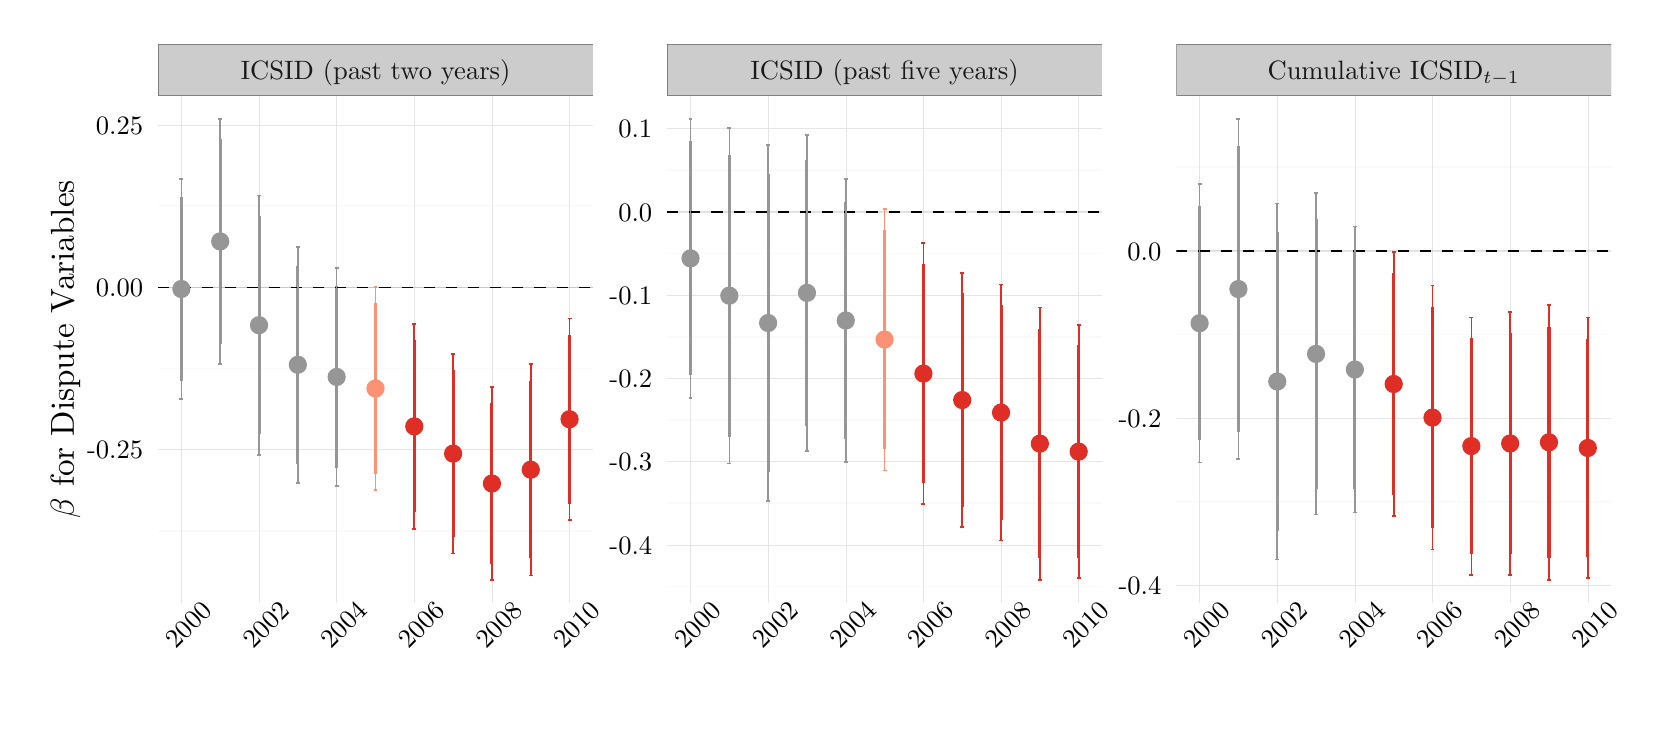
\begin{tikzpicture}[x=1pt,y=1pt]
\definecolor[named]{drawColor}{rgb}{0.00,0.00,0.00}
\definecolor[named]{fillColor}{rgb}{1.00,1.00,1.00}
\fill[color=fillColor,] (0,0) rectangle (578.16,252.94);
\begin{scope}
\path[clip] (  0.00,  0.00) rectangle (578.16,252.94);
\end{scope}
\begin{scope}
\path[clip] (  0.00,  0.00) rectangle (578.16,252.94);
\end{scope}
\begin{scope}
\path[clip] (  0.00,  0.00) rectangle (578.16,252.94);
\end{scope}
\begin{scope}
\path[clip] (  0.00,  0.00) rectangle (578.16,252.94);
\end{scope}
\begin{scope}
\path[clip] (  0.00,  0.00) rectangle (578.16,252.94);
\end{scope}
\begin{scope}
\path[clip] (  0.00,  0.00) rectangle (578.16,252.94);
\end{scope}
\begin{scope}
\path[clip] (  0.00,  0.00) rectangle (578.16,252.94);
\end{scope}
\begin{scope}
\path[clip] (  0.00,  0.00) rectangle (578.16,252.94);
\end{scope}
\begin{scope}
\path[clip] (  0.00,  0.00) rectangle (578.16,252.94);
\end{scope}
\begin{scope}
\path[clip] (  0.00,  0.00) rectangle (578.16,252.94);
\end{scope}
\begin{scope}
\path[clip] (  0.00,  0.00) rectangle (578.16,252.94);
\end{scope}
\begin{scope}
\path[clip] (  0.00,  0.00) rectangle (578.16,252.94);
\end{scope}
\begin{scope}
\path[clip] (  0.00,  0.00) rectangle (578.16,252.94);
\end{scope}
\begin{scope}
\path[clip] (  0.00,  0.00) rectangle (578.16,252.94);
\end{scope}
\begin{scope}
\path[clip] (  0.00,  0.00) rectangle (578.16,252.94);
\end{scope}
\begin{scope}
\path[clip] (  0.00,  0.00) rectangle (578.16,252.94);
\end{scope}
\begin{scope}
\path[clip] (  0.00,  0.00) rectangle (578.16,252.94);
\end{scope}
\begin{scope}
\path[clip] (  0.00,  0.00) rectangle (578.16,252.94);
\end{scope}
\begin{scope}
\path[clip] (  0.00,  0.00) rectangle (578.16,252.94);
\definecolor[named]{drawColor}{rgb}{1.00,1.00,1.00}
\definecolor[named]{fillColor}{rgb}{1.00,1.00,1.00}

\draw[color=drawColor,line width= 0.6pt,line cap=round,line join=round,fill=fillColor,] ( -0.00,  0.00) rectangle (578.16,252.94);
\end{scope}
\begin{scope}
\path[clip] (  0.00,  0.00) rectangle (578.16,252.94);
\end{scope}
\begin{scope}
\path[clip] ( 47.13, 45.11) rectangle (204.23,228.33);
\definecolor[named]{fillColor}{rgb}{1.00,1.00,1.00}

\draw[fill=fillColor,draw opacity=0.00,] ( 47.13, 45.11) rectangle (204.23,228.33);
\definecolor[named]{drawColor}{rgb}{0.98,0.98,0.98}

\draw[color=drawColor,line width= 0.6pt,line join=round,fill opacity=0.00,] ( 47.13, 71.11) --
	(204.23, 71.11);

\draw[color=drawColor,line width= 0.6pt,line join=round,fill opacity=0.00,] ( 47.13,129.76) --
	(204.23,129.76);

\draw[color=drawColor,line width= 0.6pt,line join=round,fill opacity=0.00,] ( 47.13,188.41) --
	(204.23,188.41);
\definecolor[named]{drawColor}{rgb}{0.90,0.90,0.90}

\draw[color=drawColor,line width= 0.2pt,line join=round,fill opacity=0.00,] ( 47.13,100.44) --
	(204.23,100.44);

\draw[color=drawColor,line width= 0.2pt,line join=round,fill opacity=0.00,] ( 47.13,159.09) --
	(204.23,159.09);

\draw[color=drawColor,line width= 0.2pt,line join=round,fill opacity=0.00,] ( 47.13,217.74) --
	(204.23,217.74);

\draw[color=drawColor,line width= 0.2pt,line join=round,fill opacity=0.00,] ( 55.54, 45.11) --
	( 55.54,228.33);

\draw[color=drawColor,line width= 0.2pt,line join=round,fill opacity=0.00,] ( 83.60, 45.11) --
	( 83.60,228.33);

\draw[color=drawColor,line width= 0.2pt,line join=round,fill opacity=0.00,] (111.65, 45.11) --
	(111.65,228.33);

\draw[color=drawColor,line width= 0.2pt,line join=round,fill opacity=0.00,] (139.70, 45.11) --
	(139.70,228.33);

\draw[color=drawColor,line width= 0.2pt,line join=round,fill opacity=0.00,] (167.76, 45.11) --
	(167.76,228.33);

\draw[color=drawColor,line width= 0.2pt,line join=round,fill opacity=0.00,] (195.81, 45.11) --
	(195.81,228.33);
\definecolor[named]{drawColor}{rgb}{0.59,0.59,0.59}
\definecolor[named]{fillColor}{rgb}{0.59,0.59,0.59}

\draw[color=drawColor,line width= 0.3pt,line join=round,fill=fillColor,fill opacity=0.30,draw opacity=0.30,] ( 55.54,118.77) -- ( 55.54,198.25);

\draw[color=drawColor,line width= 0.3pt,line join=round,fill=fillColor,fill opacity=0.30,draw opacity=0.30,] ( 69.57,131.39) -- ( 69.57,220.01);

\draw[color=drawColor,line width= 0.3pt,line join=round,fill=fillColor,fill opacity=0.30,draw opacity=0.30,] ( 83.60, 98.54) -- ( 83.60,192.32);

\draw[color=drawColor,line width= 0.3pt,line join=round,fill=fillColor,fill opacity=0.30,draw opacity=0.30,] ( 97.62, 88.47) -- ( 97.62,173.80);

\draw[color=drawColor,line width= 0.3pt,line join=round,fill=fillColor,fill opacity=0.30,draw opacity=0.30,] (111.65, 87.39) -- (111.65,166.06);
\definecolor[named]{drawColor}{rgb}{0.99,0.57,0.45}
\definecolor[named]{fillColor}{rgb}{0.99,0.57,0.45}

\draw[color=drawColor,line width= 0.3pt,line join=round,fill=fillColor,fill opacity=0.30,draw opacity=0.30,] (125.68, 85.90) -- (125.68,159.23);
\definecolor[named]{drawColor}{rgb}{0.87,0.18,0.15}
\definecolor[named]{fillColor}{rgb}{0.87,0.18,0.15}

\draw[color=drawColor,line width= 0.3pt,line join=round,fill=fillColor,fill opacity=0.30,draw opacity=0.30,] (139.70, 71.80) -- (139.70,145.96);

\draw[color=drawColor,line width= 0.3pt,line join=round,fill=fillColor,fill opacity=0.30,draw opacity=0.30,] (153.73, 62.95) -- (153.73,135.10);

\draw[color=drawColor,line width= 0.3pt,line join=round,fill=fillColor,fill opacity=0.30,draw opacity=0.30,] (167.76, 53.44) -- (167.76,123.00);

\draw[color=drawColor,line width= 0.3pt,line join=round,fill=fillColor,fill opacity=0.30,draw opacity=0.30,] (181.79, 55.04) -- (181.79,131.37);

\draw[color=drawColor,line width= 0.3pt,line join=round,fill=fillColor,fill opacity=0.30,draw opacity=0.30,] (195.81, 75.10) -- (195.81,147.80);
\definecolor[named]{drawColor}{rgb}{0.59,0.59,0.59}
\definecolor[named]{fillColor}{rgb}{0.59,0.59,0.59}

\draw[color=drawColor,line width= 1.1pt,line join=round,fill=fillColor,] ( 55.54,125.15) -- ( 55.54,191.86);

\draw[color=drawColor,line width= 1.1pt,line join=round,fill=fillColor,] ( 69.57,138.51) -- ( 69.57,212.88);

\draw[color=drawColor,line width= 1.1pt,line join=round,fill=fillColor,] ( 83.60,106.07) -- ( 83.60,184.78);

\draw[color=drawColor,line width= 1.1pt,line join=round,fill=fillColor,] ( 97.62, 95.33) -- ( 97.62,166.94);

\draw[color=drawColor,line width= 1.1pt,line join=round,fill=fillColor,] (111.65, 93.72) -- (111.65,159.73);
\definecolor[named]{drawColor}{rgb}{0.99,0.57,0.45}
\definecolor[named]{fillColor}{rgb}{0.99,0.57,0.45}

\draw[color=drawColor,line width= 1.1pt,line join=round,fill=fillColor,] (125.68, 91.80) -- (125.68,153.34);
\definecolor[named]{drawColor}{rgb}{0.87,0.18,0.15}
\definecolor[named]{fillColor}{rgb}{0.87,0.18,0.15}

\draw[color=drawColor,line width= 1.1pt,line join=round,fill=fillColor,] (139.70, 77.76) -- (139.70,140.00);

\draw[color=drawColor,line width= 1.1pt,line join=round,fill=fillColor,] (153.73, 68.75) -- (153.73,129.30);

\draw[color=drawColor,line width= 1.1pt,line join=round,fill=fillColor,] (167.76, 59.03) -- (167.76,117.40);

\draw[color=drawColor,line width= 1.1pt,line join=round,fill=fillColor,] (181.79, 61.18) -- (181.79,125.23);

\draw[color=drawColor,line width= 1.1pt,line join=round,fill=fillColor,] (195.81, 80.95) -- (195.81,141.95);
\definecolor[named]{drawColor}{rgb}{0.00,0.00,0.00}
\definecolor[named]{fillColor}{rgb}{0.00,0.00,0.00}

\draw[color=drawColor,line width= 0.6pt,dash pattern=on 4pt off 4pt ,line join=round,fill=fillColor,] ( 47.13,159.09) -- (204.23,159.09);
\definecolor[named]{drawColor}{rgb}{0.59,0.59,0.59}
\definecolor[named]{fillColor}{rgb}{0.59,0.59,0.59}

\draw[color=drawColor,line width= 0.4pt,line cap=round,line join=round,fill=fillColor,] ( 55.54,158.51) circle (  3.09);

\draw[color=drawColor,line width= 0.4pt,line cap=round,line join=round,fill=fillColor,] ( 69.57,175.70) circle (  3.09);

\draw[color=drawColor,line width= 0.4pt,line cap=round,line join=round,fill=fillColor,] ( 83.60,145.43) circle (  3.09);

\draw[color=drawColor,line width= 0.4pt,line cap=round,line join=round,fill=fillColor,] ( 97.62,131.13) circle (  3.09);

\draw[color=drawColor,line width= 0.4pt,line cap=round,line join=round,fill=fillColor,] (111.65,126.73) circle (  3.09);
\definecolor[named]{drawColor}{rgb}{0.99,0.57,0.45}
\definecolor[named]{fillColor}{rgb}{0.99,0.57,0.45}

\draw[color=drawColor,line width= 0.4pt,line cap=round,line join=round,fill=fillColor,] (125.68,122.57) circle (  3.09);
\definecolor[named]{drawColor}{rgb}{0.87,0.18,0.15}
\definecolor[named]{fillColor}{rgb}{0.87,0.18,0.15}

\draw[color=drawColor,line width= 0.4pt,line cap=round,line join=round,fill=fillColor,] (139.70,108.88) circle (  3.09);

\draw[color=drawColor,line width= 0.4pt,line cap=round,line join=round,fill=fillColor,] (153.73, 99.03) circle (  3.09);

\draw[color=drawColor,line width= 0.4pt,line cap=round,line join=round,fill=fillColor,] (167.76, 88.22) circle (  3.09);

\draw[color=drawColor,line width= 0.4pt,line cap=round,line join=round,fill=fillColor,] (181.79, 93.20) circle (  3.09);

\draw[color=drawColor,line width= 0.4pt,line cap=round,line join=round,fill=fillColor,] (195.81,111.45) circle (  3.09);
\definecolor[named]{drawColor}{rgb}{0.59,0.59,0.59}
\definecolor[named]{fillColor}{rgb}{0.59,0.59,0.59}

\draw[color=drawColor,line width= 0.6pt,line join=round,] ( 54.84,198.25) --
	( 56.24,198.25);

\draw[color=drawColor,line width= 0.6pt,line join=round,] ( 55.54,198.25) --
	( 55.54,118.77);

\draw[color=drawColor,line width= 0.6pt,line join=round,] ( 54.84,118.77) --
	( 56.24,118.77);

\draw[color=drawColor,line width= 0.6pt,line join=round,] ( 68.87,220.01) --
	( 70.27,220.01);

\draw[color=drawColor,line width= 0.6pt,line join=round,] ( 69.57,220.01) --
	( 69.57,131.39);

\draw[color=drawColor,line width= 0.6pt,line join=round,] ( 68.87,131.39) --
	( 70.27,131.39);

\draw[color=drawColor,line width= 0.6pt,line join=round,] ( 82.90,192.32) --
	( 84.30,192.32);

\draw[color=drawColor,line width= 0.6pt,line join=round,] ( 83.60,192.32) --
	( 83.60, 98.54);

\draw[color=drawColor,line width= 0.6pt,line join=round,] ( 82.90, 98.54) --
	( 84.30, 98.54);

\draw[color=drawColor,line width= 0.6pt,line join=round,] ( 96.92,173.80) --
	( 98.33,173.80);

\draw[color=drawColor,line width= 0.6pt,line join=round,] ( 97.62,173.80) --
	( 97.62, 88.47);

\draw[color=drawColor,line width= 0.6pt,line join=round,] ( 96.92, 88.47) --
	( 98.33, 88.47);

\draw[color=drawColor,line width= 0.6pt,line join=round,] (110.95,166.06) --
	(112.35,166.06);

\draw[color=drawColor,line width= 0.6pt,line join=round,] (111.65,166.06) --
	(111.65, 87.39);

\draw[color=drawColor,line width= 0.6pt,line join=round,] (110.95, 87.39) --
	(112.35, 87.39);
\definecolor[named]{drawColor}{rgb}{0.99,0.57,0.45}
\definecolor[named]{fillColor}{rgb}{0.99,0.57,0.45}

\draw[color=drawColor,line width= 0.6pt,line join=round,] (124.98,159.23) --
	(126.38,159.23);

\draw[color=drawColor,line width= 0.6pt,line join=round,] (125.68,159.23) --
	(125.68, 85.90);

\draw[color=drawColor,line width= 0.6pt,line join=round,] (124.98, 85.90) --
	(126.38, 85.90);
\definecolor[named]{drawColor}{rgb}{0.87,0.18,0.15}
\definecolor[named]{fillColor}{rgb}{0.87,0.18,0.15}

\draw[color=drawColor,line width= 0.6pt,line join=round,] (139.00,145.96) --
	(140.41,145.96);

\draw[color=drawColor,line width= 0.6pt,line join=round,] (139.70,145.96) --
	(139.70, 71.80);

\draw[color=drawColor,line width= 0.6pt,line join=round,] (139.00, 71.80) --
	(140.41, 71.80);

\draw[color=drawColor,line width= 0.6pt,line join=round,] (153.03,135.10) --
	(154.43,135.10);

\draw[color=drawColor,line width= 0.6pt,line join=round,] (153.73,135.10) --
	(153.73, 62.95);

\draw[color=drawColor,line width= 0.6pt,line join=round,] (153.03, 62.95) --
	(154.43, 62.95);

\draw[color=drawColor,line width= 0.6pt,line join=round,] (167.06,123.00) --
	(168.46,123.00);

\draw[color=drawColor,line width= 0.6pt,line join=round,] (167.76,123.00) --
	(167.76, 53.44);

\draw[color=drawColor,line width= 0.6pt,line join=round,] (167.06, 53.44) --
	(168.46, 53.44);

\draw[color=drawColor,line width= 0.6pt,line join=round,] (181.08,131.37) --
	(182.49,131.37);

\draw[color=drawColor,line width= 0.6pt,line join=round,] (181.79,131.37) --
	(181.79, 55.04);

\draw[color=drawColor,line width= 0.6pt,line join=round,] (181.08, 55.04) --
	(182.49, 55.04);

\draw[color=drawColor,line width= 0.6pt,line join=round,] (195.11,147.80) --
	(196.51,147.80);

\draw[color=drawColor,line width= 0.6pt,line join=round,] (195.81,147.80) --
	(195.81, 75.10);

\draw[color=drawColor,line width= 0.6pt,line join=round,] (195.11, 75.10) --
	(196.51, 75.10);
\end{scope}
\begin{scope}
\path[clip] (  0.00,  0.00) rectangle (578.16,252.94);
\end{scope}
\begin{scope}
\path[clip] (231.09, 45.11) rectangle (388.19,228.33);
\definecolor[named]{fillColor}{rgb}{1.00,1.00,1.00}

\draw[fill=fillColor,draw opacity=0.00,] (231.09, 45.11) rectangle (388.19,228.33);
\definecolor[named]{drawColor}{rgb}{0.98,0.98,0.98}

\draw[color=drawColor,line width= 0.6pt,line join=round,fill opacity=0.00,] (231.09, 50.98) --
	(388.19, 50.98);

\draw[color=drawColor,line width= 0.6pt,line join=round,fill opacity=0.00,] (231.09, 81.06) --
	(388.19, 81.06);

\draw[color=drawColor,line width= 0.6pt,line join=round,fill opacity=0.00,] (231.09,111.14) --
	(388.19,111.14);

\draw[color=drawColor,line width= 0.6pt,line join=round,fill opacity=0.00,] (231.09,141.23) --
	(388.19,141.23);

\draw[color=drawColor,line width= 0.6pt,line join=round,fill opacity=0.00,] (231.09,171.31) --
	(388.19,171.31);

\draw[color=drawColor,line width= 0.6pt,line join=round,fill opacity=0.00,] (231.09,201.39) --
	(388.19,201.39);
\definecolor[named]{drawColor}{rgb}{0.90,0.90,0.90}

\draw[color=drawColor,line width= 0.2pt,line join=round,fill opacity=0.00,] (231.09, 66.02) --
	(388.19, 66.02);

\draw[color=drawColor,line width= 0.2pt,line join=round,fill opacity=0.00,] (231.09, 96.10) --
	(388.19, 96.10);

\draw[color=drawColor,line width= 0.2pt,line join=round,fill opacity=0.00,] (231.09,126.18) --
	(388.19,126.18);

\draw[color=drawColor,line width= 0.2pt,line join=round,fill opacity=0.00,] (231.09,156.27) --
	(388.19,156.27);

\draw[color=drawColor,line width= 0.2pt,line join=round,fill opacity=0.00,] (231.09,186.35) --
	(388.19,186.35);

\draw[color=drawColor,line width= 0.2pt,line join=round,fill opacity=0.00,] (231.09,216.43) --
	(388.19,216.43);

\draw[color=drawColor,line width= 0.2pt,line join=round,fill opacity=0.00,] (239.51, 45.11) --
	(239.51,228.33);

\draw[color=drawColor,line width= 0.2pt,line join=round,fill opacity=0.00,] (267.56, 45.11) --
	(267.56,228.33);

\draw[color=drawColor,line width= 0.2pt,line join=round,fill opacity=0.00,] (295.62, 45.11) --
	(295.62,228.33);

\draw[color=drawColor,line width= 0.2pt,line join=round,fill opacity=0.00,] (323.67, 45.11) --
	(323.67,228.33);

\draw[color=drawColor,line width= 0.2pt,line join=round,fill opacity=0.00,] (351.72, 45.11) --
	(351.72,228.33);

\draw[color=drawColor,line width= 0.2pt,line join=round,fill opacity=0.00,] (379.78, 45.11) --
	(379.78,228.33);
\definecolor[named]{drawColor}{rgb}{0.59,0.59,0.59}
\definecolor[named]{fillColor}{rgb}{0.59,0.59,0.59}

\draw[color=drawColor,line width= 0.3pt,line join=round,fill=fillColor,fill opacity=0.30,draw opacity=0.30,] (239.51,119.16) -- (239.51,220.01);

\draw[color=drawColor,line width= 0.3pt,line join=round,fill=fillColor,fill opacity=0.30,draw opacity=0.30,] (253.54, 95.44) -- (253.54,216.76);

\draw[color=drawColor,line width= 0.3pt,line join=round,fill=fillColor,fill opacity=0.30,draw opacity=0.30,] (267.56, 81.90) -- (267.56,210.54);

\draw[color=drawColor,line width= 0.3pt,line join=round,fill=fillColor,fill opacity=0.30,draw opacity=0.30,] (281.59, 99.99) -- (281.59,214.25);

\draw[color=drawColor,line width= 0.3pt,line join=round,fill=fillColor,fill opacity=0.30,draw opacity=0.30,] (295.62, 96.02) -- (295.62,198.24);
\definecolor[named]{drawColor}{rgb}{0.99,0.57,0.45}
\definecolor[named]{fillColor}{rgb}{0.99,0.57,0.45}

\draw[color=drawColor,line width= 0.3pt,line join=round,fill=fillColor,fill opacity=0.30,draw opacity=0.30,] (309.64, 92.97) -- (309.64,187.53);
\definecolor[named]{drawColor}{rgb}{0.87,0.18,0.15}
\definecolor[named]{fillColor}{rgb}{0.87,0.18,0.15}

\draw[color=drawColor,line width= 0.3pt,line join=round,fill=fillColor,fill opacity=0.30,draw opacity=0.30,] (323.67, 80.85) -- (323.67,175.06);

\draw[color=drawColor,line width= 0.3pt,line join=round,fill=fillColor,fill opacity=0.30,draw opacity=0.30,] (337.70, 72.47) -- (337.70,164.31);

\draw[color=drawColor,line width= 0.3pt,line join=round,fill=fillColor,fill opacity=0.30,draw opacity=0.30,] (351.72, 67.57) -- (351.72,160.14);

\draw[color=drawColor,line width= 0.3pt,line join=round,fill=fillColor,fill opacity=0.30,draw opacity=0.30,] (365.75, 53.44) -- (365.75,151.82);

\draw[color=drawColor,line width= 0.3pt,line join=round,fill=fillColor,fill opacity=0.30,draw opacity=0.30,] (379.78, 54.03) -- (379.78,145.45);
\definecolor[named]{drawColor}{rgb}{0.59,0.59,0.59}
\definecolor[named]{fillColor}{rgb}{0.59,0.59,0.59}

\draw[color=drawColor,line width= 1.1pt,line join=round,fill=fillColor,] (239.51,127.27) -- (239.51,211.90);

\draw[color=drawColor,line width= 1.1pt,line join=round,fill=fillColor,] (253.54,105.19) -- (253.54,207.01);

\draw[color=drawColor,line width= 1.1pt,line join=round,fill=fillColor,] (267.56, 92.24) -- (267.56,200.20);

\draw[color=drawColor,line width= 1.1pt,line join=round,fill=fillColor,] (281.59,109.18) -- (281.59,205.06);

\draw[color=drawColor,line width= 1.1pt,line join=round,fill=fillColor,] (295.62,104.23) -- (295.62,190.02);
\definecolor[named]{drawColor}{rgb}{0.99,0.57,0.45}
\definecolor[named]{fillColor}{rgb}{0.99,0.57,0.45}

\draw[color=drawColor,line width= 1.1pt,line join=round,fill=fillColor,] (309.64,100.57) -- (309.64,179.93);
\definecolor[named]{drawColor}{rgb}{0.87,0.18,0.15}
\definecolor[named]{fillColor}{rgb}{0.87,0.18,0.15}

\draw[color=drawColor,line width= 1.1pt,line join=round,fill=fillColor,] (323.67, 88.42) -- (323.67,167.49);

\draw[color=drawColor,line width= 1.1pt,line join=round,fill=fillColor,] (337.70, 79.85) -- (337.70,156.92);

\draw[color=drawColor,line width= 1.1pt,line join=round,fill=fillColor,] (351.72, 75.01) -- (351.72,152.70);

\draw[color=drawColor,line width= 1.1pt,line join=round,fill=fillColor,] (365.75, 61.35) -- (365.75,143.91);

\draw[color=drawColor,line width= 1.1pt,line join=round,fill=fillColor,] (379.78, 61.38) -- (379.78,138.10);
\definecolor[named]{drawColor}{rgb}{0.00,0.00,0.00}
\definecolor[named]{fillColor}{rgb}{0.00,0.00,0.00}

\draw[color=drawColor,line width= 0.6pt,dash pattern=on 4pt off 4pt ,line join=round,fill=fillColor,] (231.09,186.35) -- (388.19,186.35);
\definecolor[named]{drawColor}{rgb}{0.59,0.59,0.59}
\definecolor[named]{fillColor}{rgb}{0.59,0.59,0.59}

\draw[color=drawColor,line width= 0.4pt,line cap=round,line join=round,fill=fillColor,] (239.51,169.58) circle (  3.09);

\draw[color=drawColor,line width= 0.4pt,line cap=round,line join=round,fill=fillColor,] (253.54,156.10) circle (  3.09);

\draw[color=drawColor,line width= 0.4pt,line cap=round,line join=round,fill=fillColor,] (267.56,146.22) circle (  3.09);

\draw[color=drawColor,line width= 0.4pt,line cap=round,line join=round,fill=fillColor,] (281.59,157.12) circle (  3.09);

\draw[color=drawColor,line width= 0.4pt,line cap=round,line join=round,fill=fillColor,] (295.62,147.13) circle (  3.09);
\definecolor[named]{drawColor}{rgb}{0.99,0.57,0.45}
\definecolor[named]{fillColor}{rgb}{0.99,0.57,0.45}

\draw[color=drawColor,line width= 0.4pt,line cap=round,line join=round,fill=fillColor,] (309.64,140.25) circle (  3.09);
\definecolor[named]{drawColor}{rgb}{0.87,0.18,0.15}
\definecolor[named]{fillColor}{rgb}{0.87,0.18,0.15}

\draw[color=drawColor,line width= 0.4pt,line cap=round,line join=round,fill=fillColor,] (323.67,127.95) circle (  3.09);

\draw[color=drawColor,line width= 0.4pt,line cap=round,line join=round,fill=fillColor,] (337.70,118.39) circle (  3.09);

\draw[color=drawColor,line width= 0.4pt,line cap=round,line join=round,fill=fillColor,] (351.72,113.85) circle (  3.09);

\draw[color=drawColor,line width= 0.4pt,line cap=round,line join=round,fill=fillColor,] (365.75,102.63) circle (  3.09);

\draw[color=drawColor,line width= 0.4pt,line cap=round,line join=round,fill=fillColor,] (379.78, 99.74) circle (  3.09);
\definecolor[named]{drawColor}{rgb}{0.59,0.59,0.59}
\definecolor[named]{fillColor}{rgb}{0.59,0.59,0.59}

\draw[color=drawColor,line width= 0.6pt,line join=round,] (238.81,220.01) --
	(240.21,220.01);

\draw[color=drawColor,line width= 0.6pt,line join=round,] (239.51,220.01) --
	(239.51,119.16);

\draw[color=drawColor,line width= 0.6pt,line join=round,] (238.81,119.16) --
	(240.21,119.16);

\draw[color=drawColor,line width= 0.6pt,line join=round,] (252.83,216.76) --
	(254.24,216.76);

\draw[color=drawColor,line width= 0.6pt,line join=round,] (253.54,216.76) --
	(253.54, 95.44);

\draw[color=drawColor,line width= 0.6pt,line join=round,] (252.83, 95.44) --
	(254.24, 95.44);

\draw[color=drawColor,line width= 0.6pt,line join=round,] (266.86,210.54) --
	(268.26,210.54);

\draw[color=drawColor,line width= 0.6pt,line join=round,] (267.56,210.54) --
	(267.56, 81.90);

\draw[color=drawColor,line width= 0.6pt,line join=round,] (266.86, 81.90) --
	(268.26, 81.90);

\draw[color=drawColor,line width= 0.6pt,line join=round,] (280.89,214.25) --
	(282.29,214.25);

\draw[color=drawColor,line width= 0.6pt,line join=round,] (281.59,214.25) --
	(281.59, 99.99);

\draw[color=drawColor,line width= 0.6pt,line join=round,] (280.89, 99.99) --
	(282.29, 99.99);

\draw[color=drawColor,line width= 0.6pt,line join=round,] (294.91,198.24) --
	(296.32,198.24);

\draw[color=drawColor,line width= 0.6pt,line join=round,] (295.62,198.24) --
	(295.62, 96.02);

\draw[color=drawColor,line width= 0.6pt,line join=round,] (294.91, 96.02) --
	(296.32, 96.02);
\definecolor[named]{drawColor}{rgb}{0.99,0.57,0.45}
\definecolor[named]{fillColor}{rgb}{0.99,0.57,0.45}

\draw[color=drawColor,line width= 0.6pt,line join=round,] (308.94,187.53) --
	(310.34,187.53);

\draw[color=drawColor,line width= 0.6pt,line join=round,] (309.64,187.53) --
	(309.64, 92.97);

\draw[color=drawColor,line width= 0.6pt,line join=round,] (308.94, 92.97) --
	(310.34, 92.97);
\definecolor[named]{drawColor}{rgb}{0.87,0.18,0.15}
\definecolor[named]{fillColor}{rgb}{0.87,0.18,0.15}

\draw[color=drawColor,line width= 0.6pt,line join=round,] (322.97,175.06) --
	(324.37,175.06);

\draw[color=drawColor,line width= 0.6pt,line join=round,] (323.67,175.06) --
	(323.67, 80.85);

\draw[color=drawColor,line width= 0.6pt,line join=round,] (322.97, 80.85) --
	(324.37, 80.85);

\draw[color=drawColor,line width= 0.6pt,line join=round,] (337.00,164.31) --
	(338.40,164.31);

\draw[color=drawColor,line width= 0.6pt,line join=round,] (337.70,164.31) --
	(337.70, 72.47);

\draw[color=drawColor,line width= 0.6pt,line join=round,] (337.00, 72.47) --
	(338.40, 72.47);

\draw[color=drawColor,line width= 0.6pt,line join=round,] (351.02,160.14) --
	(352.43,160.14);

\draw[color=drawColor,line width= 0.6pt,line join=round,] (351.72,160.14) --
	(351.72, 67.57);

\draw[color=drawColor,line width= 0.6pt,line join=round,] (351.02, 67.57) --
	(352.43, 67.57);

\draw[color=drawColor,line width= 0.6pt,line join=round,] (365.05,151.82) --
	(366.45,151.82);

\draw[color=drawColor,line width= 0.6pt,line join=round,] (365.75,151.82) --
	(365.75, 53.44);

\draw[color=drawColor,line width= 0.6pt,line join=round,] (365.05, 53.44) --
	(366.45, 53.44);

\draw[color=drawColor,line width= 0.6pt,line join=round,] (379.08,145.45) --
	(380.48,145.45);

\draw[color=drawColor,line width= 0.6pt,line join=round,] (379.78,145.45) --
	(379.78, 54.03);

\draw[color=drawColor,line width= 0.6pt,line join=round,] (379.08, 54.03) --
	(380.48, 54.03);
\end{scope}
\begin{scope}
\path[clip] (  0.00,  0.00) rectangle (578.16,252.94);
\end{scope}
\begin{scope}
\path[clip] (415.06, 45.11) rectangle (572.16,228.33);
\definecolor[named]{fillColor}{rgb}{1.00,1.00,1.00}

\draw[fill=fillColor,draw opacity=0.00,] (415.06, 45.11) rectangle (572.16,228.33);
\definecolor[named]{drawColor}{rgb}{0.98,0.98,0.98}

\draw[color=drawColor,line width= 0.6pt,line join=round,fill opacity=0.00,] (415.06, 81.53) --
	(572.16, 81.53);

\draw[color=drawColor,line width= 0.6pt,line join=round,fill opacity=0.00,] (415.06,142.02) --
	(572.16,142.02);

\draw[color=drawColor,line width= 0.6pt,line join=round,fill opacity=0.00,] (415.06,202.52) --
	(572.16,202.52);
\definecolor[named]{drawColor}{rgb}{0.90,0.90,0.90}

\draw[color=drawColor,line width= 0.2pt,line join=round,fill opacity=0.00,] (415.06, 51.28) --
	(572.16, 51.28);

\draw[color=drawColor,line width= 0.2pt,line join=round,fill opacity=0.00,] (415.06,111.78) --
	(572.16,111.78);

\draw[color=drawColor,line width= 0.2pt,line join=round,fill opacity=0.00,] (415.06,172.27) --
	(572.16,172.27);

\draw[color=drawColor,line width= 0.2pt,line join=round,fill opacity=0.00,] (423.47, 45.11) --
	(423.47,228.33);

\draw[color=drawColor,line width= 0.2pt,line join=round,fill opacity=0.00,] (451.53, 45.11) --
	(451.53,228.33);

\draw[color=drawColor,line width= 0.2pt,line join=round,fill opacity=0.00,] (479.58, 45.11) --
	(479.58,228.33);

\draw[color=drawColor,line width= 0.2pt,line join=round,fill opacity=0.00,] (507.64, 45.11) --
	(507.64,228.33);

\draw[color=drawColor,line width= 0.2pt,line join=round,fill opacity=0.00,] (535.69, 45.11) --
	(535.69,228.33);

\draw[color=drawColor,line width= 0.2pt,line join=round,fill opacity=0.00,] (563.74, 45.11) --
	(563.74,228.33);
\definecolor[named]{drawColor}{rgb}{0.59,0.59,0.59}
\definecolor[named]{fillColor}{rgb}{0.59,0.59,0.59}

\draw[color=drawColor,line width= 0.3pt,line join=round,fill=fillColor,fill opacity=0.30,draw opacity=0.30,] (423.47, 95.81) -- (423.47,196.47);

\draw[color=drawColor,line width= 0.3pt,line join=round,fill=fillColor,fill opacity=0.30,draw opacity=0.30,] (437.50, 96.97) -- (437.50,220.01);

\draw[color=drawColor,line width= 0.3pt,line join=round,fill=fillColor,fill opacity=0.30,draw opacity=0.30,] (451.53, 60.72) -- (451.53,189.44);

\draw[color=drawColor,line width= 0.3pt,line join=round,fill=fillColor,fill opacity=0.30,draw opacity=0.30,] (465.55, 76.99) -- (465.55,193.11);

\draw[color=drawColor,line width= 0.3pt,line join=round,fill=fillColor,fill opacity=0.30,draw opacity=0.30,] (479.58, 77.78) -- (479.58,181.05);
\definecolor[named]{drawColor}{rgb}{0.87,0.18,0.15}
\definecolor[named]{fillColor}{rgb}{0.87,0.18,0.15}

\draw[color=drawColor,line width= 0.3pt,line join=round,fill=fillColor,fill opacity=0.30,draw opacity=0.30,] (493.61, 76.37) -- (493.61,171.99);

\draw[color=drawColor,line width= 0.3pt,line join=round,fill=fillColor,fill opacity=0.30,draw opacity=0.30,] (507.64, 64.38) -- (507.64,159.72);

\draw[color=drawColor,line width= 0.3pt,line join=round,fill=fillColor,fill opacity=0.30,draw opacity=0.30,] (521.66, 55.24) -- (521.66,148.25);

\draw[color=drawColor,line width= 0.3pt,line join=round,fill=fillColor,fill opacity=0.30,draw opacity=0.30,] (535.69, 55.15) -- (535.69,150.24);

\draw[color=drawColor,line width= 0.3pt,line join=round,fill=fillColor,fill opacity=0.30,draw opacity=0.30,] (549.72, 53.44) -- (549.72,152.77);

\draw[color=drawColor,line width= 0.3pt,line join=round,fill=fillColor,fill opacity=0.30,draw opacity=0.30,] (563.74, 53.96) -- (563.74,148.17);
\definecolor[named]{drawColor}{rgb}{0.59,0.59,0.59}
\definecolor[named]{fillColor}{rgb}{0.59,0.59,0.59}

\draw[color=drawColor,line width= 1.1pt,line join=round,fill=fillColor,] (423.47,103.90) -- (423.47,188.37);

\draw[color=drawColor,line width= 1.1pt,line join=round,fill=fillColor,] (437.50,106.86) -- (437.50,210.11);

\draw[color=drawColor,line width= 1.1pt,line join=round,fill=fillColor,] (451.53, 71.07) -- (451.53,179.10);

\draw[color=drawColor,line width= 1.1pt,line join=round,fill=fillColor,] (465.55, 86.33) -- (465.55,183.78);

\draw[color=drawColor,line width= 1.1pt,line join=round,fill=fillColor,] (479.58, 86.08) -- (479.58,172.75);
\definecolor[named]{drawColor}{rgb}{0.87,0.18,0.15}
\definecolor[named]{fillColor}{rgb}{0.87,0.18,0.15}

\draw[color=drawColor,line width= 1.1pt,line join=round,fill=fillColor,] (493.61, 84.06) -- (493.61,164.30);

\draw[color=drawColor,line width= 1.1pt,line join=round,fill=fillColor,] (507.64, 72.04) -- (507.64,152.06);

\draw[color=drawColor,line width= 1.1pt,line join=round,fill=fillColor,] (521.66, 62.72) -- (521.66,140.78);

\draw[color=drawColor,line width= 1.1pt,line join=round,fill=fillColor,] (535.69, 62.80) -- (535.69,142.60);

\draw[color=drawColor,line width= 1.1pt,line join=round,fill=fillColor,] (549.72, 61.43) -- (549.72,144.79);

\draw[color=drawColor,line width= 1.1pt,line join=round,fill=fillColor,] (563.74, 61.53) -- (563.74,140.59);
\definecolor[named]{drawColor}{rgb}{0.00,0.00,0.00}
\definecolor[named]{fillColor}{rgb}{0.00,0.00,0.00}

\draw[color=drawColor,line width= 0.6pt,dash pattern=on 4pt off 4pt ,line join=round,fill=fillColor,] (415.06,172.27) -- (572.16,172.27);
\definecolor[named]{drawColor}{rgb}{0.59,0.59,0.59}
\definecolor[named]{fillColor}{rgb}{0.59,0.59,0.59}

\draw[color=drawColor,line width= 0.4pt,line cap=round,line join=round,fill=fillColor,] (423.47,146.14) circle (  3.09);

\draw[color=drawColor,line width= 0.4pt,line cap=round,line join=round,fill=fillColor,] (437.50,158.49) circle (  3.09);

\draw[color=drawColor,line width= 0.4pt,line cap=round,line join=round,fill=fillColor,] (451.53,125.08) circle (  3.09);

\draw[color=drawColor,line width= 0.4pt,line cap=round,line join=round,fill=fillColor,] (465.55,135.05) circle (  3.09);

\draw[color=drawColor,line width= 0.4pt,line cap=round,line join=round,fill=fillColor,] (479.58,129.41) circle (  3.09);
\definecolor[named]{drawColor}{rgb}{0.87,0.18,0.15}
\definecolor[named]{fillColor}{rgb}{0.87,0.18,0.15}

\draw[color=drawColor,line width= 0.4pt,line cap=round,line join=round,fill=fillColor,] (493.61,124.18) circle (  3.09);

\draw[color=drawColor,line width= 0.4pt,line cap=round,line join=round,fill=fillColor,] (507.64,112.05) circle (  3.09);

\draw[color=drawColor,line width= 0.4pt,line cap=round,line join=round,fill=fillColor,] (521.66,101.75) circle (  3.09);

\draw[color=drawColor,line width= 0.4pt,line cap=round,line join=round,fill=fillColor,] (535.69,102.70) circle (  3.09);

\draw[color=drawColor,line width= 0.4pt,line cap=round,line join=round,fill=fillColor,] (549.72,103.11) circle (  3.09);

\draw[color=drawColor,line width= 0.4pt,line cap=round,line join=round,fill=fillColor,] (563.74,101.06) circle (  3.09);
\definecolor[named]{drawColor}{rgb}{0.59,0.59,0.59}
\definecolor[named]{fillColor}{rgb}{0.59,0.59,0.59}

\draw[color=drawColor,line width= 0.6pt,line join=round,] (422.77,196.47) --
	(424.18,196.47);

\draw[color=drawColor,line width= 0.6pt,line join=round,] (423.47,196.47) --
	(423.47, 95.81);

\draw[color=drawColor,line width= 0.6pt,line join=round,] (422.77, 95.81) --
	(424.18, 95.81);

\draw[color=drawColor,line width= 0.6pt,line join=round,] (436.80,220.01) --
	(438.20,220.01);

\draw[color=drawColor,line width= 0.6pt,line join=round,] (437.50,220.01) --
	(437.50, 96.97);

\draw[color=drawColor,line width= 0.6pt,line join=round,] (436.80, 96.97) --
	(438.20, 96.97);

\draw[color=drawColor,line width= 0.6pt,line join=round,] (450.83,189.44) --
	(452.23,189.44);

\draw[color=drawColor,line width= 0.6pt,line join=round,] (451.53,189.44) --
	(451.53, 60.72);

\draw[color=drawColor,line width= 0.6pt,line join=round,] (450.83, 60.72) --
	(452.23, 60.72);

\draw[color=drawColor,line width= 0.6pt,line join=round,] (464.85,193.11) --
	(466.26,193.11);

\draw[color=drawColor,line width= 0.6pt,line join=round,] (465.55,193.11) --
	(465.55, 76.99);

\draw[color=drawColor,line width= 0.6pt,line join=round,] (464.85, 76.99) --
	(466.26, 76.99);

\draw[color=drawColor,line width= 0.6pt,line join=round,] (478.88,181.05) --
	(480.28,181.05);

\draw[color=drawColor,line width= 0.6pt,line join=round,] (479.58,181.05) --
	(479.58, 77.78);

\draw[color=drawColor,line width= 0.6pt,line join=round,] (478.88, 77.78) --
	(480.28, 77.78);
\definecolor[named]{drawColor}{rgb}{0.87,0.18,0.15}
\definecolor[named]{fillColor}{rgb}{0.87,0.18,0.15}

\draw[color=drawColor,line width= 0.6pt,line join=round,] (492.91,171.99) --
	(494.31,171.99);

\draw[color=drawColor,line width= 0.6pt,line join=round,] (493.61,171.99) --
	(493.61, 76.37);

\draw[color=drawColor,line width= 0.6pt,line join=round,] (492.91, 76.37) --
	(494.31, 76.37);

\draw[color=drawColor,line width= 0.6pt,line join=round,] (506.93,159.72) --
	(508.34,159.72);

\draw[color=drawColor,line width= 0.6pt,line join=round,] (507.64,159.72) --
	(507.64, 64.38);

\draw[color=drawColor,line width= 0.6pt,line join=round,] (506.93, 64.38) --
	(508.34, 64.38);

\draw[color=drawColor,line width= 0.6pt,line join=round,] (520.96,148.25) --
	(522.36,148.25);

\draw[color=drawColor,line width= 0.6pt,line join=round,] (521.66,148.25) --
	(521.66, 55.24);

\draw[color=drawColor,line width= 0.6pt,line join=round,] (520.96, 55.24) --
	(522.36, 55.24);

\draw[color=drawColor,line width= 0.6pt,line join=round,] (534.99,150.24) --
	(536.39,150.24);

\draw[color=drawColor,line width= 0.6pt,line join=round,] (535.69,150.24) --
	(535.69, 55.15);

\draw[color=drawColor,line width= 0.6pt,line join=round,] (534.99, 55.15) --
	(536.39, 55.15);

\draw[color=drawColor,line width= 0.6pt,line join=round,] (549.02,152.77) --
	(550.42,152.77);

\draw[color=drawColor,line width= 0.6pt,line join=round,] (549.72,152.77) --
	(549.72, 53.44);

\draw[color=drawColor,line width= 0.6pt,line join=round,] (549.02, 53.44) --
	(550.42, 53.44);

\draw[color=drawColor,line width= 0.6pt,line join=round,] (563.04,148.17) --
	(564.45,148.17);

\draw[color=drawColor,line width= 0.6pt,line join=round,] (563.74,148.17) --
	(563.74, 53.96);

\draw[color=drawColor,line width= 0.6pt,line join=round,] (563.04, 53.96) --
	(564.45, 53.96);
\end{scope}
\begin{scope}
\path[clip] (  0.00,  0.00) rectangle (578.16,252.94);
\end{scope}
\begin{scope}
\path[clip] (  0.00,  0.00) rectangle (578.16,252.94);
\end{scope}
\begin{scope}
\path[clip] ( 47.13,228.33) rectangle (204.23,246.95);
\definecolor[named]{drawColor}{rgb}{0.50,0.50,0.50}
\definecolor[named]{fillColor}{rgb}{0.80,0.80,0.80}

\draw[color=drawColor,line width= 0.2pt,line cap=round,line join=round,fill=fillColor,] ( 47.13,228.33) rectangle (204.23,246.95);
\definecolor[named]{drawColor}{rgb}{0.10,0.10,0.10}

\node[color=drawColor,anchor=base,inner sep=0pt, outer sep=0pt, scale=  0.96] at (125.68,234.33) {ICSID (past two years)%
};
\end{scope}
\begin{scope}
\path[clip] ( 47.13,228.33) rectangle (204.23,246.95);
\end{scope}
\begin{scope}
\path[clip] (  0.00,  0.00) rectangle (578.16,252.94);
\end{scope}
\begin{scope}
\path[clip] (  0.00,  0.00) rectangle (578.16,252.94);
\end{scope}
\begin{scope}
\path[clip] (  0.00,  0.00) rectangle (578.16,252.94);
\end{scope}
\begin{scope}
\path[clip] (231.09,228.33) rectangle (388.19,246.95);
\definecolor[named]{drawColor}{rgb}{0.50,0.50,0.50}
\definecolor[named]{fillColor}{rgb}{0.80,0.80,0.80}

\draw[color=drawColor,line width= 0.2pt,line cap=round,line join=round,fill=fillColor,] (231.09,228.33) rectangle (388.19,246.95);
\definecolor[named]{drawColor}{rgb}{0.10,0.10,0.10}

\node[color=drawColor,anchor=base,inner sep=0pt, outer sep=0pt, scale=  0.96] at (309.64,234.33) {ICSID (past five years)%
};
\end{scope}
\begin{scope}
\path[clip] (231.09,228.33) rectangle (388.19,246.95);
\end{scope}
\begin{scope}
\path[clip] (  0.00,  0.00) rectangle (578.16,252.94);
\end{scope}
\begin{scope}
\path[clip] (  0.00,  0.00) rectangle (578.16,252.94);
\end{scope}
\begin{scope}
\path[clip] (  0.00,  0.00) rectangle (578.16,252.94);
\end{scope}
\begin{scope}
\path[clip] (415.06,228.33) rectangle (572.16,246.95);
\definecolor[named]{drawColor}{rgb}{0.50,0.50,0.50}
\definecolor[named]{fillColor}{rgb}{0.80,0.80,0.80}

\draw[color=drawColor,line width= 0.2pt,line cap=round,line join=round,fill=fillColor,] (415.06,228.33) rectangle (572.16,246.95);
\definecolor[named]{drawColor}{rgb}{0.10,0.10,0.10}

\node[color=drawColor,anchor=base,inner sep=0pt, outer sep=0pt, scale=  0.96] at (493.61,234.33) {Cumulative ICSID$_{t-1}$%
};
\end{scope}
\begin{scope}
\path[clip] (415.06,228.33) rectangle (572.16,246.95);
\end{scope}
\begin{scope}
\path[clip] (  0.00,  0.00) rectangle (578.16,252.94);
\end{scope}
\begin{scope}
\path[clip] (  0.00,  0.00) rectangle (578.16,252.94);
\end{scope}
\begin{scope}
\path[clip] (  0.00,  0.00) rectangle (578.16,252.94);
\end{scope}
\begin{scope}
\path[clip] (  0.00,  0.00) rectangle (578.16,252.94);
\end{scope}
\begin{scope}
\path[clip] (  0.00,  0.00) rectangle (578.16,252.94);
\end{scope}
\begin{scope}
\path[clip] (  0.00,  0.00) rectangle (578.16,252.94);
\end{scope}
\begin{scope}
\path[clip] (  0.00,  0.00) rectangle (578.16,252.94);
\definecolor[named]{drawColor}{rgb}{0.00,0.00,0.00}

\node[color=drawColor,anchor=base east,inner sep=0pt, outer sep=0pt, scale=  0.96] at ( 41.73, 97.13) {-0.25%
};

\node[color=drawColor,anchor=base east,inner sep=0pt, outer sep=0pt, scale=  0.96] at ( 41.73,155.78) {0.00%
};

\node[color=drawColor,anchor=base east,inner sep=0pt, outer sep=0pt, scale=  0.96] at ( 41.73,214.43) {0.25%
};
\end{scope}
\begin{scope}
\path[clip] (  0.00,  0.00) rectangle (578.16,252.94);
\end{scope}
\begin{scope}
\path[clip] (  0.00,  0.00) rectangle (578.16,252.94);
\end{scope}
\begin{scope}
\path[clip] (  0.00,  0.00) rectangle (578.16,252.94);
\end{scope}
\begin{scope}
\path[clip] (  0.00,  0.00) rectangle (578.16,252.94);
\end{scope}
\begin{scope}
\path[clip] (  0.00,  0.00) rectangle (578.16,252.94);
\end{scope}
\begin{scope}
\path[clip] (  0.00,  0.00) rectangle (578.16,252.94);
\end{scope}
\begin{scope}
\path[clip] (  0.00,  0.00) rectangle (578.16,252.94);
\end{scope}
\begin{scope}
\path[clip] (  0.00,  0.00) rectangle (578.16,252.94);
\end{scope}
\begin{scope}
\path[clip] (  0.00,  0.00) rectangle (578.16,252.94);
\end{scope}
\begin{scope}
\path[clip] (  0.00,  0.00) rectangle (578.16,252.94);
\definecolor[named]{drawColor}{rgb}{0.00,0.00,0.00}

\node[color=drawColor,anchor=base east,inner sep=0pt, outer sep=0pt, scale=  0.96] at (225.69, 62.72) {-0.4%
};

\node[color=drawColor,anchor=base east,inner sep=0pt, outer sep=0pt, scale=  0.96] at (225.69, 92.80) {-0.3%
};

\node[color=drawColor,anchor=base east,inner sep=0pt, outer sep=0pt, scale=  0.96] at (225.69,122.88) {-0.2%
};

\node[color=drawColor,anchor=base east,inner sep=0pt, outer sep=0pt, scale=  0.96] at (225.69,152.96) {-0.1%
};

\node[color=drawColor,anchor=base east,inner sep=0pt, outer sep=0pt, scale=  0.96] at (225.69,183.04) {0.0%
};

\node[color=drawColor,anchor=base east,inner sep=0pt, outer sep=0pt, scale=  0.96] at (225.69,213.12) {0.1%
};
\end{scope}
\begin{scope}
\path[clip] (  0.00,  0.00) rectangle (578.16,252.94);
\end{scope}
\begin{scope}
\path[clip] (  0.00,  0.00) rectangle (578.16,252.94);
\end{scope}
\begin{scope}
\path[clip] (  0.00,  0.00) rectangle (578.16,252.94);
\end{scope}
\begin{scope}
\path[clip] (  0.00,  0.00) rectangle (578.16,252.94);
\end{scope}
\begin{scope}
\path[clip] (  0.00,  0.00) rectangle (578.16,252.94);
\end{scope}
\begin{scope}
\path[clip] (  0.00,  0.00) rectangle (578.16,252.94);
\end{scope}
\begin{scope}
\path[clip] (  0.00,  0.00) rectangle (578.16,252.94);
\end{scope}
\begin{scope}
\path[clip] (  0.00,  0.00) rectangle (578.16,252.94);
\end{scope}
\begin{scope}
\path[clip] (  0.00,  0.00) rectangle (578.16,252.94);
\end{scope}
\begin{scope}
\path[clip] (  0.00,  0.00) rectangle (578.16,252.94);
\definecolor[named]{drawColor}{rgb}{0.00,0.00,0.00}

\node[color=drawColor,anchor=base east,inner sep=0pt, outer sep=0pt, scale=  0.96] at (409.66, 47.97) {-0.4%
};

\node[color=drawColor,anchor=base east,inner sep=0pt, outer sep=0pt, scale=  0.96] at (409.66,108.47) {-0.2%
};

\node[color=drawColor,anchor=base east,inner sep=0pt, outer sep=0pt, scale=  0.96] at (409.66,168.97) {0.0%
};
\end{scope}
\begin{scope}
\path[clip] (  0.00,  0.00) rectangle (578.16,252.94);
\end{scope}
\begin{scope}
\path[clip] (  0.00,  0.00) rectangle (578.16,252.94);
\end{scope}
\begin{scope}
\path[clip] (  0.00,  0.00) rectangle (578.16,252.94);
\end{scope}
\begin{scope}
\path[clip] (  0.00,  0.00) rectangle (578.16,252.94);
\end{scope}
\begin{scope}
\path[clip] (  0.00,  0.00) rectangle (578.16,252.94);
\end{scope}
\begin{scope}
\path[clip] (  0.00,  0.00) rectangle (578.16,252.94);
\end{scope}
\begin{scope}
\path[clip] (  0.00,  0.00) rectangle (578.16,252.94);
\end{scope}
\begin{scope}
\path[clip] (  0.00,  0.00) rectangle (578.16,252.94);
\end{scope}
\begin{scope}
\path[clip] (  0.00,  0.00) rectangle (578.16,252.94);
\end{scope}
\begin{scope}
\path[clip] (  0.00,  0.00) rectangle (578.16,252.94);
\end{scope}
\begin{scope}
\path[clip] (  0.00,  0.00) rectangle (578.16,252.94);
\end{scope}
\begin{scope}
\path[clip] (  0.00,  0.00) rectangle (578.16,252.94);
\definecolor[named]{drawColor}{rgb}{0.00,0.00,0.00}

\node[rotate= 45.00,color=drawColor,anchor=base,inner sep=0pt, outer sep=0pt, scale=  0.96] at ( 60.22, 35.04) {2000%
};

\node[rotate= 45.00,color=drawColor,anchor=base,inner sep=0pt, outer sep=0pt, scale=  0.96] at ( 88.27, 35.04) {2002%
};

\node[rotate= 45.00,color=drawColor,anchor=base,inner sep=0pt, outer sep=0pt, scale=  0.96] at (116.33, 35.04) {2004%
};

\node[rotate= 45.00,color=drawColor,anchor=base,inner sep=0pt, outer sep=0pt, scale=  0.96] at (144.38, 35.04) {2006%
};

\node[rotate= 45.00,color=drawColor,anchor=base,inner sep=0pt, outer sep=0pt, scale=  0.96] at (172.43, 35.04) {2008%
};

\node[rotate= 45.00,color=drawColor,anchor=base,inner sep=0pt, outer sep=0pt, scale=  0.96] at (200.49, 35.04) {2010%
};
\end{scope}
\begin{scope}
\path[clip] (  0.00,  0.00) rectangle (578.16,252.94);
\end{scope}
\begin{scope}
\path[clip] (  0.00,  0.00) rectangle (578.16,252.94);
\end{scope}
\begin{scope}
\path[clip] (  0.00,  0.00) rectangle (578.16,252.94);
\end{scope}
\begin{scope}
\path[clip] (  0.00,  0.00) rectangle (578.16,252.94);
\end{scope}
\begin{scope}
\path[clip] (  0.00,  0.00) rectangle (578.16,252.94);
\end{scope}
\begin{scope}
\path[clip] (  0.00,  0.00) rectangle (578.16,252.94);
\end{scope}
\begin{scope}
\path[clip] (  0.00,  0.00) rectangle (578.16,252.94);
\end{scope}
\begin{scope}
\path[clip] (  0.00,  0.00) rectangle (578.16,252.94);
\end{scope}
\begin{scope}
\path[clip] (  0.00,  0.00) rectangle (578.16,252.94);
\end{scope}
\begin{scope}
\path[clip] (  0.00,  0.00) rectangle (578.16,252.94);
\definecolor[named]{drawColor}{rgb}{0.00,0.00,0.00}

\node[rotate= 45.00,color=drawColor,anchor=base,inner sep=0pt, outer sep=0pt, scale=  0.96] at (244.18, 35.04) {2000%
};

\node[rotate= 45.00,color=drawColor,anchor=base,inner sep=0pt, outer sep=0pt, scale=  0.96] at (272.24, 35.04) {2002%
};

\node[rotate= 45.00,color=drawColor,anchor=base,inner sep=0pt, outer sep=0pt, scale=  0.96] at (300.29, 35.04) {2004%
};

\node[rotate= 45.00,color=drawColor,anchor=base,inner sep=0pt, outer sep=0pt, scale=  0.96] at (328.35, 35.04) {2006%
};

\node[rotate= 45.00,color=drawColor,anchor=base,inner sep=0pt, outer sep=0pt, scale=  0.96] at (356.40, 35.04) {2008%
};

\node[rotate= 45.00,color=drawColor,anchor=base,inner sep=0pt, outer sep=0pt, scale=  0.96] at (384.45, 35.04) {2010%
};
\end{scope}
\begin{scope}
\path[clip] (  0.00,  0.00) rectangle (578.16,252.94);
\end{scope}
\begin{scope}
\path[clip] (  0.00,  0.00) rectangle (578.16,252.94);
\end{scope}
\begin{scope}
\path[clip] (  0.00,  0.00) rectangle (578.16,252.94);
\end{scope}
\begin{scope}
\path[clip] (  0.00,  0.00) rectangle (578.16,252.94);
\end{scope}
\begin{scope}
\path[clip] (  0.00,  0.00) rectangle (578.16,252.94);
\end{scope}
\begin{scope}
\path[clip] (  0.00,  0.00) rectangle (578.16,252.94);
\end{scope}
\begin{scope}
\path[clip] (  0.00,  0.00) rectangle (578.16,252.94);
\end{scope}
\begin{scope}
\path[clip] (  0.00,  0.00) rectangle (578.16,252.94);
\end{scope}
\begin{scope}
\path[clip] (  0.00,  0.00) rectangle (578.16,252.94);
\end{scope}
\begin{scope}
\path[clip] (  0.00,  0.00) rectangle (578.16,252.94);
\definecolor[named]{drawColor}{rgb}{0.00,0.00,0.00}

\node[rotate= 45.00,color=drawColor,anchor=base,inner sep=0pt, outer sep=0pt, scale=  0.96] at (428.15, 35.04) {2000%
};

\node[rotate= 45.00,color=drawColor,anchor=base,inner sep=0pt, outer sep=0pt, scale=  0.96] at (456.20, 35.04) {2002%
};

\node[rotate= 45.00,color=drawColor,anchor=base,inner sep=0pt, outer sep=0pt, scale=  0.96] at (484.26, 35.04) {2004%
};

\node[rotate= 45.00,color=drawColor,anchor=base,inner sep=0pt, outer sep=0pt, scale=  0.96] at (512.31, 35.04) {2006%
};

\node[rotate= 45.00,color=drawColor,anchor=base,inner sep=0pt, outer sep=0pt, scale=  0.96] at (540.36, 35.04) {2008%
};

\node[rotate= 45.00,color=drawColor,anchor=base,inner sep=0pt, outer sep=0pt, scale=  0.96] at (568.42, 35.04) {2010%
};
\end{scope}
\begin{scope}
\path[clip] (  0.00,  0.00) rectangle (578.16,252.94);
\end{scope}
\begin{scope}
\path[clip] (  0.00,  0.00) rectangle (578.16,252.94);
\end{scope}
\begin{scope}
\path[clip] (  0.00,  0.00) rectangle (578.16,252.94);
\end{scope}
\begin{scope}
\path[clip] (  0.00,  0.00) rectangle (578.16,252.94);
\end{scope}
\begin{scope}
\path[clip] (  0.00,  0.00) rectangle (578.16,252.94);
\end{scope}
\begin{scope}
\path[clip] (  0.00,  0.00) rectangle (578.16,252.94);
\definecolor[named]{drawColor}{rgb}{0.00,0.00,0.00}

\node[rotate= 90.00,color=drawColor,anchor=base,inner sep=0pt, outer sep=0pt, scale=  1.20] at ( 16.66,136.72) {$\beta$ for Dispute Variables%
};
\end{scope}
\begin{scope}
\path[clip] (  0.00,  0.00) rectangle (578.16,252.94);
\end{scope}
\begin{scope}
\path[clip] (  0.00,  0.00) rectangle (578.16,252.94);
\end{scope}
\begin{scope}
\path[clip] (  0.00,  0.00) rectangle (578.16,252.94);
\end{scope}
\begin{scope}
\path[clip] (  0.00,  0.00) rectangle (578.16,252.94);
\end{scope}
\end{tikzpicture}
}
	\caption*{Note: Each point here designates the coefficient estimate for a disputes variable in that year. The thick line represents the 90\% confidence interval around that point estimate, while the longer, thin line represents the 95\% confidence interval. All the covariates used in the initial model shown in Table \ref{tab:dispRepLevel} were included in these pooled models as controls.}
\end{figure}
\FloatBarrier

\section*{Short Versus Long Term Effects}

A key limitation of the preceding set of results is that they do not directly address the issue of reputational change nor allow us to distinguish between the short and long-term effects of alleged treaty violations. For this reason, we probe the impact of investment disputes further below on the basis of an error correction model (ECM). Whereas prior research has assumed that investment disputes lead investors to reassess political risk, our central theoretical expectation is that reputational costs only emerge slowly over time with the accumulation of arbitral claims and the growth of information about state behavior. In other words, the arguments relating state reputation to treaty compliance are arguably best understood as reflecting long-term equilibria rather than transitory or short-term effects. To the extent that the impact of dispute involvement is heavily dependent on information flows, we also expect that reputational damage is more likely in the post-2006 period than earlier. Finally, given the relative visibility and transparency of the ICSID, we expect more reputational damage from arbitration at the ICSID than alternative venues.

Utilizing the same set of cases and variables as in the previous analysis, we assess these expectations on the basis of a model that includes the lagged dependent variable as well as both changes and lags of the independent variables as follows:

\begin{equation}
\Delta Y_{i,t} = \alpha + \Delta X_{i,t-1} \beta + \Phi(Y_{i,t-1} - X_{i,t-1} \gamma) + \epsilon_{i,t}
\end{equation}

where $Y_{i,t}$ is the reputation of country $i$ during year $t$, $\Delta$ is a first difference operator, $X$ is a vector of independent variables, and $\epsilon_{i,t}$, is an error term. The dependent variable is thus the change in state reputation in a given year and the independent variables include lagged investment reputation, the lagged values of the independent variables, and lagged changes in the independent variables. Rewriting the equation in the form in which it is actually estimated, yields

\begin{equation}
\Delta Y_{i,t} = \alpha + Y_{i,t-1} \beta_{1} + \Delta X_{i,t-1} \beta_{2} + X_{i, t-1} \beta_{3} + \epsilon_{i,t}
\end{equation}

in which $\beta_{1}$ is the same as $\Phi$ in the error correction version of the equation, $\beta_{2}$ equivalent to $\beta$, and $\Phi(Y_{i,t-1})$ is rendered by $\beta_{3}$. The short-term relationship between the registration of arbitral claims and reputation is thus captured by $\beta_{2}$  and the longer-term relationship by $\beta_{3}$.

Given problems of heteroskedasticity associated with cross-sectional time series research designs, as well as the relatively high ratio of panels to periods, the models are estimated with OLS and panel-corrected standard errors in accordance with the recommendations of \citeauthor{beck:katz:1995}.\footnote{\citet{beck:katz:1995}} The estimations are also corrected for panel-specific autocorrelation and country and time fixed effects to eliminate bias arising from omitted or unmeasured variables, which may not be completely exogenous with respect to other explanatory variables.

The estimates for changes in investment reputation are presented in Table \ref{tab:ecm}. Beginning with the control variables, we see results that are weaker and only partially consistent with those reported above in Table \ref{tab:dispRepLevel}. The evidence again suggests that GDP growth, population, and internal and external stability matter to reputation; but the other coefficients are statistically weak, with the exception of the coefficient for lagged reputation, which underlines the tendency for investment profile ratings to remain relatively stable over time. 

For the variables of central theoretical interest, changes in dispute involvement and lagged levels of accumulated dispute involvement, the coefficients are decidedly weak. In accordance with theoretical expectation, in none of the columns are short-term increases in the number of arbitral claims registered against a state in the prior year statistically significant. Consistent with our earlier analysis, we also find that investor-state disputes had no reputational impact over the 1987-2006 period. With the analysis extended to cover the post-2006 period, however, the coefficients for cumulative dispute involvement at the ICSID becomes statistically significant. This finding further underlines the importance of information availability and the relative transparency of dispute settlement processes for reputational sanctioning. 
% \newpage

\begin{table}[ht]
\vspace{1cm}
\centering
{\footnotesize
\caption{The Impact of Investor-State Disputes on International Investment Risk Profile}
\label{tab:ecm}
\begin{tabular}{lr@{} lr@{}lr@{}lr@{}lr@{}}
	\hline\hline
	~ & \multicolumn{4}{c}{ICSID} & \multicolumn{4}{c}{All Treaty Based Disputes} \\
	~ & \multicolumn{2}{c}{1987-2006} & \multicolumn{2}{c}{1987-2014} & \multicolumn{2}{c}{1987-2006} & \multicolumn{2}{c}{1987-2014} \\
	\hline
  $\Delta$Disputes & -0&.016 & -0&.011 & -0&.004 & -0&.004 \\
~ & (0&.026) & (0&.015) & (0&.014) & (0&.009) \\
  Disputes$_{t-1}$ & -0&.004 & -0&.003$^{\ast}$ & -0&.002 & -0&.001 \\
  ~ & (0&.003) &  (0&.001) & (0&.002) & (0&.001) \\
  \multirow{2}{*}{$\Delta$Log(GDP)} & 6&.692$^{\ast}$ & 5&.140$^{\ast}$ & 6&.585$^{\ast}$ & 5&.060$^{\ast}$ \\
  & (3&.187) & (2&.259) & (3&.185) & (2&.258) \\
  \multirow{2}{*}{Log(GDP)$_{t-1}$} & -0&.059 & -0&.022 & -0&.055 & -0&.020\\
  & (0&.075) & (0&.049) & (0&.076) & (0&.049) \\
  \multirow{2}{*}{$\Delta$Log(Population)} & 67&.285$^{\ast\ast}$ & 53&.966$^{\ast\ast}$ & 67&.924$^{\ast\ast}$ & 54&.273$^{\ast\ast}$ \\
  & (20&.765) & (12&.915) & (20&.804) & (12&.935)\\
  \multirow{2}{*}{Log(Population)$_{t-1}$} & -0&.019 & -0&.026 & -0&.024 & -0&.027 \\
  & (0&.181) & (0&.073) & (0&.182) & (0&.073) \\
  \multirow{2}{*}{$\Delta$Log(Inflation)} & -0&.049 &  -0&.055 &  -0&.049 &  -0&.055 \\
  & (0&.058) &  (0&.039) &  (0&.058) &  (0&.039) \\
  \multirow{2}{*}{Log(Inflation)$_{t-1}$} & 0&.031 &  0&.031 &  0&.031 &  0&.031$^{\ast}$ \\
  & (0&.020) &  (0&.016) &  (0&.020) &  (0&.016) \\
  \multirow{2}{*}{$\Delta$Internal Stability} & 0&.014 & 0&.015 &  0&.014 &  0&.016 \\
  & (0&.020) &  (0&.017) &  (0&.020) &  (0&.017) \\
  \multirow{2}{*}{Internal Stability$_{t-1}$} & 0&.015$^{\ast\ast}$ &  0&.011$^{\ast\ast}$ &  0&.015$^{\ast\ast}$ &  0&.011$^{\ast\ast}$ \\
  & (0&.006) &  (0&.004) &  (0&.006) &  (0&.004) \\
  \multirow{2}{*}{$\Delta$External Stability} & 0&.084$^{\ast\ast}$ & 0&.088$^{\ast\ast}$ &  0&.084$^{\ast\ast}$ &  0&.088$^{\ast\ast}$ \\
  & (0&.026) &  (0&.024) &  (0&.026) &  (0&.024) \\
  \multirow{2}{*}{External Stability$_{t-1}$} & -0&.002 &  0&.000 &  -0&.002 &  0&.000 \\
  & (0&.005) &  (0&.004) &  (0&.005) &  (0&.004) \\
  \multirow{2}{*}{$\Delta$Ratified BITs} & 0&.002 &  0&.000 &  0&.003 &  0&.000 \\
  & (0&.008) &  (0&.008) &  (0&.008) &  (0&.008) \\
  \multirow{2}{*}{Ratified BITs$_{t-1}$} & -0&.000 & -0&.000 &  -0&.000 & -0&.000 \\
  & (0&.001) & (0&.001) &  (0&.001) &  (0&.001) \\
  \multirow{2}{*}{$\Delta$Capital Openness} & 0&.000 & 0&.000 &  0&.000 &  0&.000 \\
  & (0&.002) &  (0&.002) &  (0&.002) &  (0&.002) \\
  \multirow{2}{*}{Capital Openness$_{t-1}$} & 0&.004 & -0&.001 &  0&.004 &  -0&.001 \\
  & (0&.010) & (0&.007) & (0&.010) & (0&.007) \\
  \multirow{2}{*}{$\Delta$Polity} & -0&.003 & -0&.002 &  -0&.003 & - 0&.002  \\
  & (0&.002) & (0&.002) &  (0&.002) &  (0&.002) \\
  \multirow{2}{*}{Polity$_{t-1}$} & 0&.001 & 0&.001 &  0&.001 &  0&.001 \\
  & (0&.001) & (0&.000) &  (0&.001) &  (0&.000) \\
    Investment & -0&.095$^{\ast\ast}$ & -0&.079$^{\ast\ast}$ & -0&.094$^{\ast\ast}$ & -0&.079$^{\ast\ast}$ \\
  $\;\;$Profile$_{t-1}$ & (0&.012) & (0&.008) & (0&.012) & (0&.008) \\
	\hline
	$n$ & 1,&708 & 2,&499 & 1,&708 & 2,&499 \\
	$N$ & 1&01 & 1&01 & 1&01 & 1&01 \\
	$R^{2}$ & 0&.38 & 0&.35 & 0&.38 & 0&.35 \\
	\hline\hline
\end{tabular}
\caption*{Note: Dispute variables succeeded by ${t-1}$ measure the lagged cumulative total of disputes; variables preceded by $\Delta$ measure percentage changes. OLS estimates with fixed effects and panel-corrected standard errors in parentheses. Coefficients for time and country dummy variables not shown.}
}
\end{table}
\FloatBarrier

% \newpage

Estimating the substantive effects of dispute involvement on the basis of the error correction form of the model presented above helps to clarify these results. Drawing on the coefficients for ICSID treaty-based disputes over the 1987-2014 period, for example, it can be calculated that with all other variables held constant the registration of a new arbitral claim against a state will only lead to a 0.01 point decline in investment reputation over the short run, which is roughly equivalent to a 0.1 percent decrease relative to the mean value of reputation for the set of cases under consideration. Although reputation will continue to decline further over time by an additional 0.003 points, the costs of an individual investor-state dispute are still not very significant substantively. Even for the registration of three new ICSID disputes in a single year, the short-term impact is only an estimated 0.03 point decline in reputation (roughly 0.5 percent) with a further adjustment over the long run of 0.01. 

\section*{Conclusion}

This paper makes an original contribution to the growing body of literature on international investor-state disputes by systematically studying their consequences for both FDI flows and investment reputation over the full 1987--2014 time period. Whereas prior research has claimed that involvement in treaty-based investment dispute arbitration is predictably translated into reduced foreign direct investment flows, we find no evidence of such an effect. We therefore turn to the analysis of reputational damage, which is the mechanism presumed to be brought into play by perceptions that a state has violated its treaty commitments. Drawing upon an original dataset that covers the investor-state dispute involvement of lower and middle income countries both at the ICSID and other international venues, we analyze the impact of investment disputes on investment reputation as well as changes in that reputation over the 1987-2014 period. Contrary to the expectations generated by the theoretical literature on international political economy, as well as prior research on ISDS, our research suggests that the reputational costs of investment dispute involvement are restricted and heavily dependent on information flows. 

Focusing initially upon the impact of disputes registered over the prior two years, our evidence indicates that investor-state disputes have a distinctly modest and contingent impact on reputation. Observable reputational differences revolve around observations for the post-2006 period during which access to information about dispute settlement processes exploded, both in response to changes in the rules governing international arbitration and mounting international publicity about ISDS. Exploring the impact of arbitral claims on changes in investment reputation on the basis of an error correction model, we find very similar results. Reputational shifts are completely unrelated to short-term increases in the number of challenges registered against a state. More significant is the record of dispute involvement accumulated by a state over the long run, particularly at the ICSID; but these results again revolve around the inclusion of observations for the post 2006-period.

Taken together our three sets of findings on the impact of disputes on foreign investment, investment reputation, and changes in investment reputation challenge the conclusions of prior research focusing on disputes registered at the ICSID between 1984 and 2006. Only in the post-2006 period have disputes manifested a reputational impact. Thus whereas the logic underlying the credible commitment story espoused in the political economy literature assumes that states incur statistically and substantively significant costs from allegations that they have violated their international agreements, we show that these costs are dependent on institutional design and information flows.

These findings have significant implications for the broader body of literature on international institutions. Existing theory assumes that formal international commitments automatically raise the ex post cost of defection, thereby creating incentives for states to comply with their treaty obligations. Our analysis significantly modifies this expectation by suggesting that the strength of the incentives for compliance vary with the monitoring, sanctioning, and enforcement mechanisms brought into play by particular sets of international institutions. Under the current ISDS regime, the monitoring of treaty compliance is externalized to individual private firms and ad hoc arbitral tribunals, whose deliberations are limited to the facts of a particular case, unpredictable, and often less than transparent. Notwithstanding the legal powers enjoyed by investors under international treaty agreements, the reputational risks of state involvement in ISDS processes have been accordingly attenuated and dependent upon information costs. It is only since 2006, when important shifts begin to take place in the access of investors to information about dispute processes, that the reputational costs of dispute involvement began to become significant. The central implication for future research is that reputational mechanisms for effective enforcement of international commitments are fundamentally dependent on institutional design and associated information costs, creating room for major variations in the capacity of international commitments to constrain state actors from engaging in uncooperative behavior.


\newpage

\bibliographystyle{APSR}
\bibliography{dispRepRefs}

% Insert in tables and figures

% \processdelayedfloats 

\newpage

\section*{Appendix}
\label{appendix}

\appendix
\setcounter{figure}{0} \renewcommand{\thefigure}{A.\arabic{figure}}
\setcounter{table}{0} \renewcommand{\thetable}{A.\arabic{table}}

\subsection*{Allee \& Peinhardt 2011 Analysis}

The difference between our results and those of Allee and Peinhardt's (2011) result from the way in which they logged the FDI variable. In doing so, they disregard the fact that logarithms of zero and negative numbers are not defined and therefore registered as missing in most statistical programs. As a result, they mistakenly exclude a notable number of country-year observations with negative or zero flows. Given their argument about the adverse reputational ramifications of ICSID disputes involvement on FDI flows, one could argue that the observations with negative flows are the most relevant portion of their dataset. In our replication of their analysis, we correct for this error by following the simple procedure suggested by \citeauthor{li:2009}, which calls for adding a constant so that each value is greater than zero before logging.\footnote{\citet{li:2009}} 

The impact of Allee and Peinhardt's error is readily apparent in Table \ref{tab:allee}. Using their data and statistical approach, the first column of the table exactly replicates their base model that assesses the impact of pending ICSID disputes over the 1984-2007 period. In column two, we follow the exact same procedure except we add a constant to negative and zero FDI values before logging the data. Comparing the results of columns one and two, it becomes evident that after including zero and negative FDI observations, ICSID dispute involvement does not significantly affect FDI flows. The results presented in other columns of the table are consistent with this finding. Columns three and four compare the results for the effect of disputes filed in the past two years, and columns five and six use disputes filed in the past five years. In each case we see that Allee and Peinhardt's original findings do not hold after including observations with negative or zero FDI in the analysis. For reasons of space, we do not report our findings with respect to other sets of Allee and Peinhardt's results, which address the impact of ICSID disputes lost or settled over the past two and five years as well as the impact of disputes lost over the past two years controlling for pending disputes. The results for these additional estimations, however, follow the same pattern as those reported in Table \ref{tab:allee}. Estimates using unlogged FDI data are very similar. 

% \newpage

\begin{table}[ht]
\vspace{1cm}
\centering
{\footnotesize
\caption{The Impact of ICSID Arbitration on FDI Inflows}
\label{tab:allee}
\begin{tabular}{lr@{} lr@{}lr@{}lr@{}lr@{}lr@{}lr@{} }
	\hline\hline
	~ & \multicolumn{4}{c}{(1)} & \multicolumn{4}{c}{(2)} & \multicolumn{4}{c}{(3)} \\	
	~ & \multicolumn{2}{c}{A \& P} & \multicolumn{2}{c}{Corrected} & \multicolumn{2}{c}{A \& P} & \multicolumn{2}{c}{Corrected} & \multicolumn{2}{c}{A \& P} & \multicolumn{2}{c}{Corrected}
	 \\ \hline
	\multirow{2}{*}{Signed BITs} & 0&.015 & 0&.001 & 0&.015 & 0&.001 & 0&.016 & 0&.001 \\
	~ & (0&.010) & (0&.000) & (0&.009) & (0&.000) & (0&.010) & (0&.000) \\
	Pending &-0&.036 &0&.000 && && && \\
	$\;\;$Claims &(0&.011) &(0&.003) && && && \\
	Disputes filed && && &-0&.057 &-0&.000 && && \\
	$\;\;$(past 2 years) && && &(0&.018) &(0&.003) && && \\
	Disputes filed && && && && &-0&.040 &-0&.000 \\
	$\;\;$(past 5 years) && && && && &(0&.011) &(0&.002) \\
	Economic & -0&.032 & -0&.004 & -0&.031 & -0&.004 & -0&.031 & -0&.004 \\
	$\;\;$Shocks & (0&.066) & (0&.003) & (0&.065) & (0&.003) & (0&.065) & (0&.003) \\
	Political & -0&.011 & -0&.000 & -0&.011 & -0&.000 & -0&.011 & -0&.000 \\
	$\;\;$Shocks & (0&.010) & (0&.001) & (0&.010) & (0&.001) & (0&.010) &(0&.001) \\
	External & -0&.046 & -0&.003 & -0&.047 & -0&.003 & -0&.047 & -0&.003 \\
	$\;\;$Threat & (0&.026) & (0&.001) & (0&.026) & (0&.001) & (0&.026) & (0&.001) \\
	\multirow{2}{*}{Polity} & 0&.015 & -0&.000 & 0&.015 & -0&.000 & 0&.015 & -0&.000 \\
	~ & (0&.018) & (0&.001) & (0&.018) & (0&.001) & (0&.018) &(0&.001) \\
	Property & 0&.039 & -0&.001 &  0&.039 & -0&.001 &  0&.039 & -0&.001 \\
	$\;\;$Rights & (0&.021) & (0&.002) & (0&.022) & (0&.002) & (0&.022) & (0&.002) \\
	\multirow{2}{*}{Log(Population)} & 1&.30 & -0&.032 & 1&.32 & -0&.032 & 1&.31 & -0&.032 \\
	& (0&.525) & (0&.032) & (0&.525) & (0&.032) & (0&.526) & (0&.032) \\
	\multirow{2}{*}{GDP per capita} & 1&.06 & 0&.051 & 1&.05 & 0&.051 & 1&.05 & 0&.051 \\
	& (0&.265) & (0&.020) & (0&.264) & (0&.020) & (0&.264) & (0&.020) \\
	\multirow{2}{*}{GDP growth} & 0&.018 & 0&.000 & 0&.018 & 0&.000 & 0&.018 & 0&.000 \\
	& (0&.007) & (0&.000) & (0&.006) & (0&.000) & (0&.007) &(0&.000) \\
	Financial & 0&.126 & 0&.005 & 0&.127 & 0&.005 & 0&.125 & 0&.005 \\
	$\;\;$Openness & (0&.059) & (0&.004) & (0&.059) & (0&.004) & (0&.058) &(0&.004) \\
	\multirow{2}{*}{Exchange rate} & -0&.001 & 0&.000 & -0&.001 & 0&.000 & -0&.001 & 0&.000 \\
	& (0&.000) & (0&.000) & (0&.000) & (0&.000) & (0&.000) &(0&.000) \\	
	\multirow{2}{*}{World FDI} & 0&.438 & 0&.024 & 0&.430 & 0&.024 & 0&.438 & 0&.024 \\
	& (0&.072) & (0&.008) & (0&.073) & (0&.008) & (0&.073) &(0&.008) \\ \hline
	$n$ & 1,&796 & 1,&956 & 1,&796 & 1,&956 & 1,&796 & 1,&956 \\
	$N$ & 1&02 & 1&02 & 1&02 & 1&02 & 1&02 & 1&02 \\
	$R^{2}$ & 0&.52 & 0&.24 & 0&.52 & 0&.24 & 0&.52 & 0&.24 \\
	\hline\hline
\end{tabular}
\caption*{Note: All variables (except World FDI) lagged one year. Fixed-effects estimation with standard errors clustered on country. Standard errors in parentheses. }
}
\end{table}
\FloatBarrier

% \subsection*{Descriptive Statistics}

% \begin{table}[ht]
% \centering
% \caption{Descriptive Statistics}
% \label{tab:descStats}
% \begin{tabular}{lcccccc}
% 	  \hline\hline
% 	  & N & n & Mean & Std. Dev. & Min & Max \\ 
% 	  \hline
% Investment Profile & 112 & 2658 & 6.94 & 2.42 & 0.00 & 12.00 \\ 
%   All ICSID Disputes (Two Year Sum) & 112 & 2644 & 0.21 & 0.94 & 0.00 & 25.00 \\ 
%   ICSID Treaty-Based (Two Year Sum) & 112 & 2644 & 0.18 & 0.92 & 0.00 & 25.00 \\ 
%   Unsettled ICSID (Two Year Sum) & 112 & 2644 & 0.13 & 0.69 & 0.00 & 15.00 \\ 
%   ICSID-UNCTAD (Two Year Sum) & 112 & 2644 & 0.24 & 1.09 & 0.00 & 29.00 \\ 
%   \%$\Delta$ GDP & 109 & 2511 & 0.09 & 0.17 & -0.80 & 1.43 \\ 
%   Ln(Pop.) & 111 & 2627 & 16.12 & 1.60 & 12.35 & 21.02 \\ 
%   Ln(Inflation) & 108 & 2355 & 3.31 & 0.71 & -4.61 & 10.10 \\ 
%   Internal Stability & 112 & 2658 & 8.48 & 2.46 & 0.00 & 12.00 \\ 
%   Ratif. BITs & 111 & 2633 & 12.20 & 15.14 & 0.00 & 101.00 \\ 
%   Capital Openness & 107 & 2469 & -0.02 & 1.53 & -1.86 & 2.44 \\ 
%   Polity & 109 & 2583 & 11.01 & 7.09 & 0.00 & 20.00 \\ 
% 	   \hline\hline
% \end{tabular}
% \end{table}

% % \newpage

% % latex table generated in R 3.0.2 by xtable 1.7-3 package
% % Mon May 19 17:07:53 2014
% \begin{table}[ht]
% \centering
% \caption{Investor-State Disputes and International Investment Risk Profile (Using Semi-Balanced Panel, $T \; \geq 17 \;  \forall$ countries)}
% \label{tab:dispRepLevelBal}
% \begin{tabular}{lr@{} lr@{}lr@{}lr@{}lr@{}}
%   \hline\hline
%   & \multicolumn{2}{c}{All ICSID} & \multicolumn{2}{c}{ICSID} & \multicolumn{2}{c}{Unsettled$^{a}$} & \multicolumn{2}{c}{ICSID-} \\ 
%   & \multicolumn{2}{c}{Disputes} & \multicolumn{2}{c}{Treaty-Based} & \multicolumn{2}{c}{ICSID} & \multicolumn{2}{c}{UNCTAD} \\
%  \hline
% Registered Disputes$_{(t-1) + (t-2)}$ & -0&.151 & -0&.162 & -0&.218 & -0&.122 \\ 
%    & (0&.067) & (0&.076) & (0&.091) & (0&.063) \\ 
%   \%$\Delta$ GDP$_{t-1}$ & 0&.543 & 0&.543 & 0&.538 & 0&.541 \\ 
%    & (0&.246) & (0&.246) & (0&.245) & (0&.247) \\ 
%   Ln(Pop.)$_{t-1}$ & 3&.573 & 3&.559 & 3&.545 & 3&.553 \\ 
%    & (0&.602) & (0&.603) & (0&.605) & (0&.605) \\ 
%   Ln(Inflation)$_{t-1}$ & -0&.388 & -0&.388 & -0&.384 & -0&.386 \\ 
%    & (0&.112) & (0&.112) & (0&.111) & (0&.113) \\ 
%   Internal Stability$_{t-1}$ & 0&.183 & 0&.182 & 0&.183 & 0&.183 \\ 
%    & (0&.033) & (0&.033) & (0&.034) & (0&.033) \\ 
%   Ratif. BITs$_{t-1}$ & 0&.035 & 0&.035 & 0&.035 & 0&.035 \\ 
%    & (0&.011) & (0&.011) & (0&.01) & (0&.011) \\ 
%   Capital Openness$_{t-1}$ & 0&.202 & 0&.201 & 0&.202 & 0&.2 \\ 
%    & (0&.088) & (0&.088) & (0&.088) & (0&.088) \\ 
%   Polity$_{t-1}$ & 0&.034 & 0&.034 & 0&.035 & 0&.034 \\ 
%    & (0&.016) & (0&.016) & (0&.016) & (0&.016) \\ 
%    \hline
% n & 1&884 & 1&884 & 1&884 & 1&884 \\ 
%   N && 79 && 79 && 79 && 79 \\ 
%   $R^{2}$ & 0&.45 & 0&.45 & 0&.45 & 0&.45 \\ 
%   RMSE & 1&.32 & 1&.32 & 1&.32 & 1&.32 \\ 
%    \hline
% \hline
% \end{tabular}
% \caption*{Note: Fixed-effects estimation with standard errors clustered on country using a balanced panel. Standard errors in parentheses. \\ a: The ``unsettled'' category excludes treaty disputes that were resolved via settlement or discontinuation prior to ICSID arbitration.}
% \end{table}

\newpage

%\newpage
%About the authors: \\

\end{document}
\bye